\documentclass[letterpaper, 11pt, colorful, sections]{cs1515}
\title{CSCI 1515: Applied Cryptography}
\author{P. Miao}
\date{Spring 2024}

\usepackage[textsize=tiny, textwidth=18mm]{todonotes}
\setuptodonotes{color=green!20}
\usepackage{marginnote}

\makeatletter
\renewcommand{\@todonotes@drawMarginNoteWithLine}{%
\begin{tikzpicture}[remember picture, overlay, baseline=-0.75ex]%   
    \node [coordinate] (inText) {};%
\end{tikzpicture}%
\marginnote[{% Draw note in left margin
    \@todonotes@drawMarginNote%
    \@todonotes@drawLineToLeftMargin%
}]{% Draw note in right margin
    \@todonotes@drawMarginNote%
    \@todonotes@drawLineToRightMargin%
}%
}%
\makeatother

\usepackage{tablefootnote} 
\makeatletter 
\AfterEndEnvironment{mdframed}{%
 \tfn@tablefootnoteprintout% 
 \gdef\tfn@fnt{0}% 
}
\makeatother
\newcommand{\framedfootnote}{\tablefootnote}

\usepackage{cancel}
\usetikzlibrary{cd}
\numberwithin{equation}{section}

\usepackage[all,cmtip]{xy}

\usepackage[
    n,
    operators,
    advantage,
    sets,
    adversary,
    landau,
    probability,
    notions,	
    logic,
    ff,
    mm,
    primitives,
    events,
    complexity,
    oracles,
    asymptotics,
    keys]{cryptocode}
\usepackage{tkz-graph}
\graphicspath{{./images/2024/}}

% Commas in footnotes:
\let\oldFootnote\footnote
\newcommand\nextToken\relax

\renewcommand\footnote[1]{%
    \oldFootnote{#1}\futurelet\nextToken\isFootnote}

\newcommand\isFootnote{%
    \ifx\footnote\nextToken\textsuperscript{,}\fi}

% \includeonly{lectures/2023-04-13.tex, lectures/2023-04-11.tex}

\begin{document}
\maketitle
\begin{quote}
    \quad These are lecture notes for CSCI 1515: Applied Cryptography taught at \textsc{Brown University} by Peihan Miao in the Spring of 2024.

    \quad These notes were originally taken by Jiahua Chen with gracious help and input from classmates and fellow TAs. Please direct any mistakes/errata to a thread on Ed, or feel free to pull request or submit an issue to the \href{https://github.com/BrownAppliedCryptography/notes}{notes repository}.

    \quad Notes last updated \today.
\end{quote}
\tableofcontents
% \bibliographystyle{alpha}
% \bibliography{bibliography}

\newpage
%!TEX root = ../notes.tex
\section{January 24, 2024}
\label{20240124}

\subsection{Introduction}
The course homepage is at \url{https://cs.brown.edu/courses/csci1515/spring-2024/}, where you can find information such as the \href{https://docs.google.com/document/d/1lvXrMACua9Ma3n2nkLeiRmG-fmjDO1530h22EjkvQ-s/edit?usp=sharing}{syllabus}, projects, homeworks, calendar, lectures and more.

The course is offered in-person in \emph{Bio Med 202}, as well as synchronously over Zoom and recorded asynchronously (lectures posted online). Lecture attendance and participation is highly encouraged!

\textbf{EdStem} will be used for course questions, and \textbf{Gradescope} is used for assignments.

\subsubsection{Staff}

Our course staff have all taken or TA-ed the course before and are excited to help you learn!

Peihan has been at Brown for a couple of years and this was the second time she is teaching this course. Before Brown, she was at the University of Illinois Chicago. Before that, she finished her PhD at UC Berkeley in 2019 with a focus in cryptography. Afterwards, she worked in industry for a couple of years (Visa) before deciding to come back to academia. She still collaborates with industry to see what problems need to be solved in practice.

During her PhD, she started off doing more theoretical cryptography but also did internships and found applied cryptography fascinating as well. Now she works in both.

\subsubsection{Course Philosophy and Logistics}

If look up other \emph{applied} cryptography courses online or at other universities, you will find courses that have ``applied'' in their title. However, if you look at their syllabus or content, it's still mostly theoretical crypto. This may (1) deter students from learning about crypto and (2) leave a gap between theoretical crypto and crypto in practice. (2) is bad because if someone makes a mistake in the crypto domain, the consequences are often significant.

As such, it's helpful for students to get hands-on experience with cryptography:
\begin{itemize}
    \item How cryptography has been used in practice and
    \item How cryptography will be used and implemented in the future.
\end{itemize}

The closest similar course is found at Stanford, which covers theoretical crypto in the first half and more applied crypto in the second. But even that course only covers very basic crypto that are very well established. In the past 10 years or so, there are new and exciting topics in crypto that are gradually becoming more and more common which we will also cover in this course.

For this course, it will be \emph{much less} about math and proofs, and much more about how you can use these tools to do something more fun. It will be coding heavy and all projects will be implemented in C++ using crypto libraries. 

If, however, you are interested in the theoretical or mathematical side, you might consider other courses at Brown like CSCI 1510 and MATH 1580.

% For assignments: \emph{Project 0} is a warmup for C++. Projects 1 \& 2 is to develop secure communication or authentication systems using the underlying cryptographic libraries. The later project, 3, 4 \& 5 will be on more advanced topics. The first 2 are more basic that are developed in practice, and the latter ones are more experimental in practice (so this is recent research in applied cryptography). The final project will be a combination of the existing projects or a project entirely new (separate from the earlier projects, but using the same cryptographic primitives).

% Projects 1 through 5 will be accompanied with homework assignments (appropriately numbered 1 through 5) that develop a conceptual understanding of the materials.

% Projects 1 \& 2 are to be done individually, the later projects are done in pairs (you can choose to go solo if you so wish as well). You are encouraged to find partners earlier on to discuss and work with them from the beginning. You are \emph{encouraged} to communicate with your partners on projects 1 \& 2 so you gain a conceptual understanding. You should complete your own write-up and code for the first two projects, however.

There is an option to capstone this course, contact Peihan about this. It would also be best to find a partner who is also capstoning this course.

The following is the grading policy:
\begin{center}
    \begin{tabular}{@{}ll@{}}
        \toprule
        \textit{Type}      & \textit{Percentage} \\ \midrule
        Project 0          & 4\%                 \\
        Projects 1 \& 2    & 20\% (10\% each)    \\
        Projects 3, 4 \& 5 & 36\% (12\% each)    \\
        Homeworks          & 25\% (5\% each)     \\
        Final Project      & 25\%                \\ \bottomrule
    \end{tabular}
\end{center}

You have 4 total late days for \emph{projects}, of which at most two can be used on a single project. Additionally, you have 3 total late days for \emph{homeworks}, of which at most one can be used on a single homework.

All projects are independent, but collaboration is allowed and encouraged. However, you \emph{must write up your own code}.

If you're sick, let Peihan know with a Dean's note.

\subsection{What is cryptography?}

At a high level, \emph{cryptography is a set of techniques that protect sensitive or important information}.

\begin{ques*}
    Where is cryptography used in practice? What guarantees do we want in these scenarios?
\end{ques*}
\begin{itemize}
    \item Online transactions
          \begin{itemize}
              \item When you make a purchase, you might not want people to see your bank balance, what else you have purchased, etc.
              \item You also want to ensure that it was really \emph{you} who purchased the item and not somebody else i.e. authentication
          \end{itemize}
    \item Secure messaging
        \begin{itemize}
            \item End-to-end texting, iMessage
            \item We don't want anyone else to see our messages
        \end{itemize}
    \item Online voting
        \begin{itemize}
            \item Privacy of votes, validity of votes
        \end{itemize}
    \item Databases
        \begin{itemize}
            \item Secure storage
        \end{itemize}
\end{itemize}

\subsection{Secure Communication}
We'll start with the most classic form of cryptography: \emph{secure communication}.

\begin{center}
    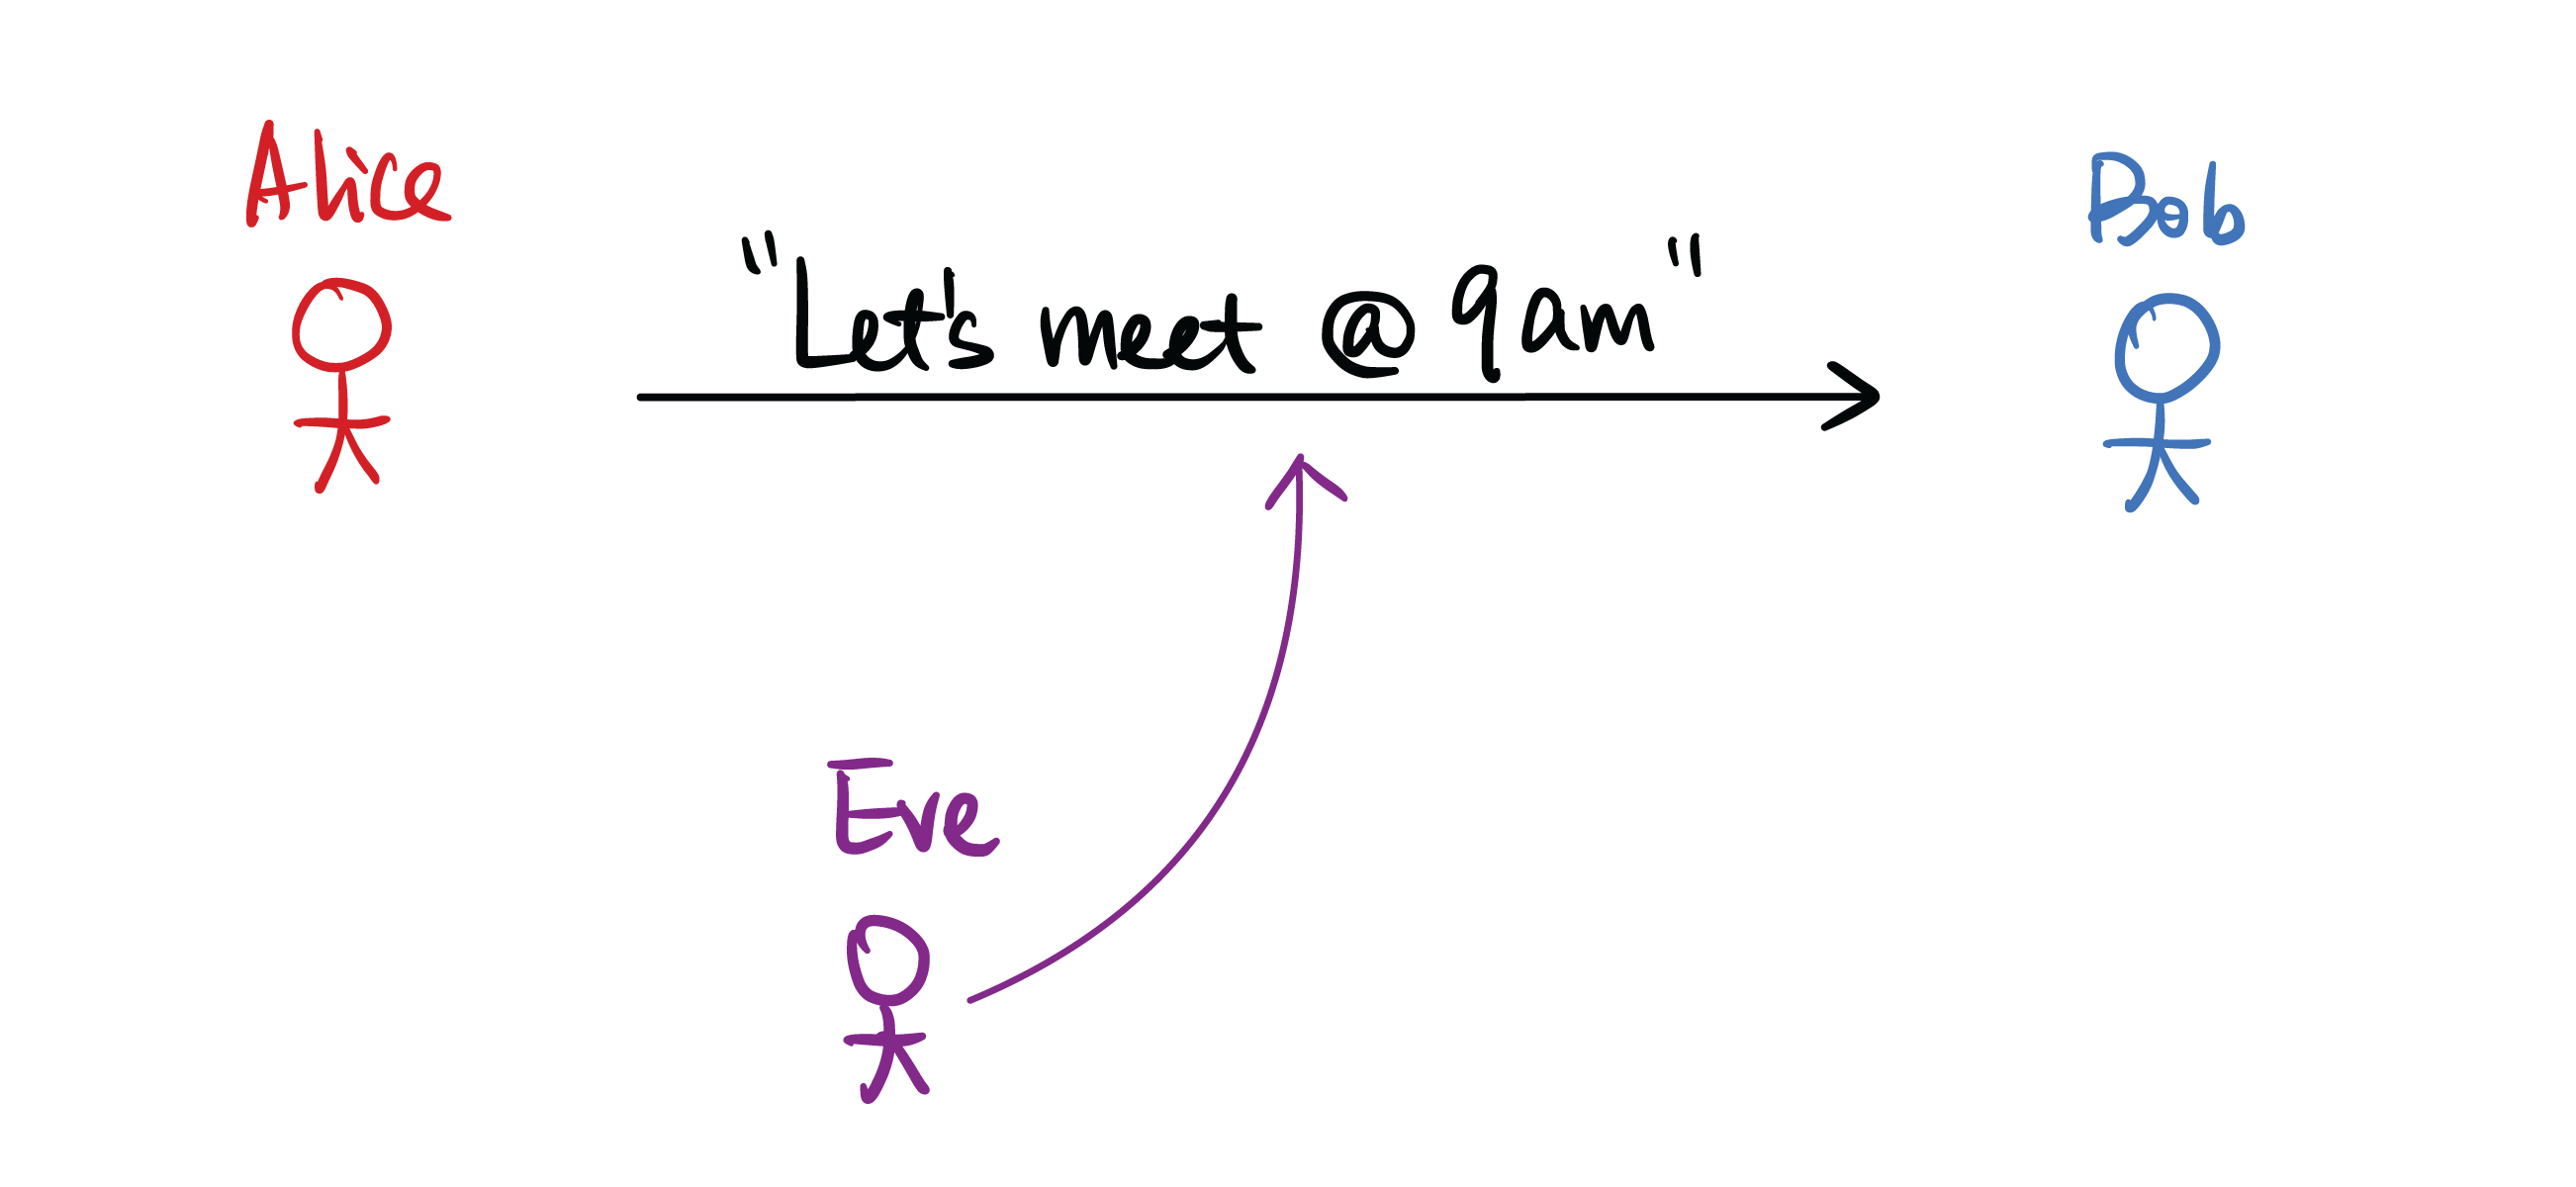
\includegraphics[width=0.8\textwidth]{images/2023-01-26/secure_computation.png}
\end{center}

Assume Alice wants to communicate to Bob ``Let's meet at 9am'', what are some security guarantees we want?

\begin{itemize}
    \item Eve cannot \emph{see} the message from Alice to Bob.
    \item Eve cannot \emph{alter} the message from Alice to Bob. 
\end{itemize}

These two guarantees are the most important guarantees! The former is called \ul{message secrecy}, the latter is called \ul{message integrity}.

\subsubsection{Message Secrecy}

\begin{definition}[Message Secrecy]
    We want cryptography to allow Alice to \emph{encrypt} the message $m$ (which we call \emph{plaintext}) by running an algorithm that produces a \emph{ciphertext} $c$. We call this an \emph{encryption scheme}.

    Bob will be able to receive the ciphertext $c$ and run a \emph{decrypt} algorithm to produce the message $m$ again. This is akin to a secure box that Alice locks up, and Bob unlocks, while Eve does not know the message. The easiest way is for Alice and Bob to agree on a shared secret key.

    \begin{center}
        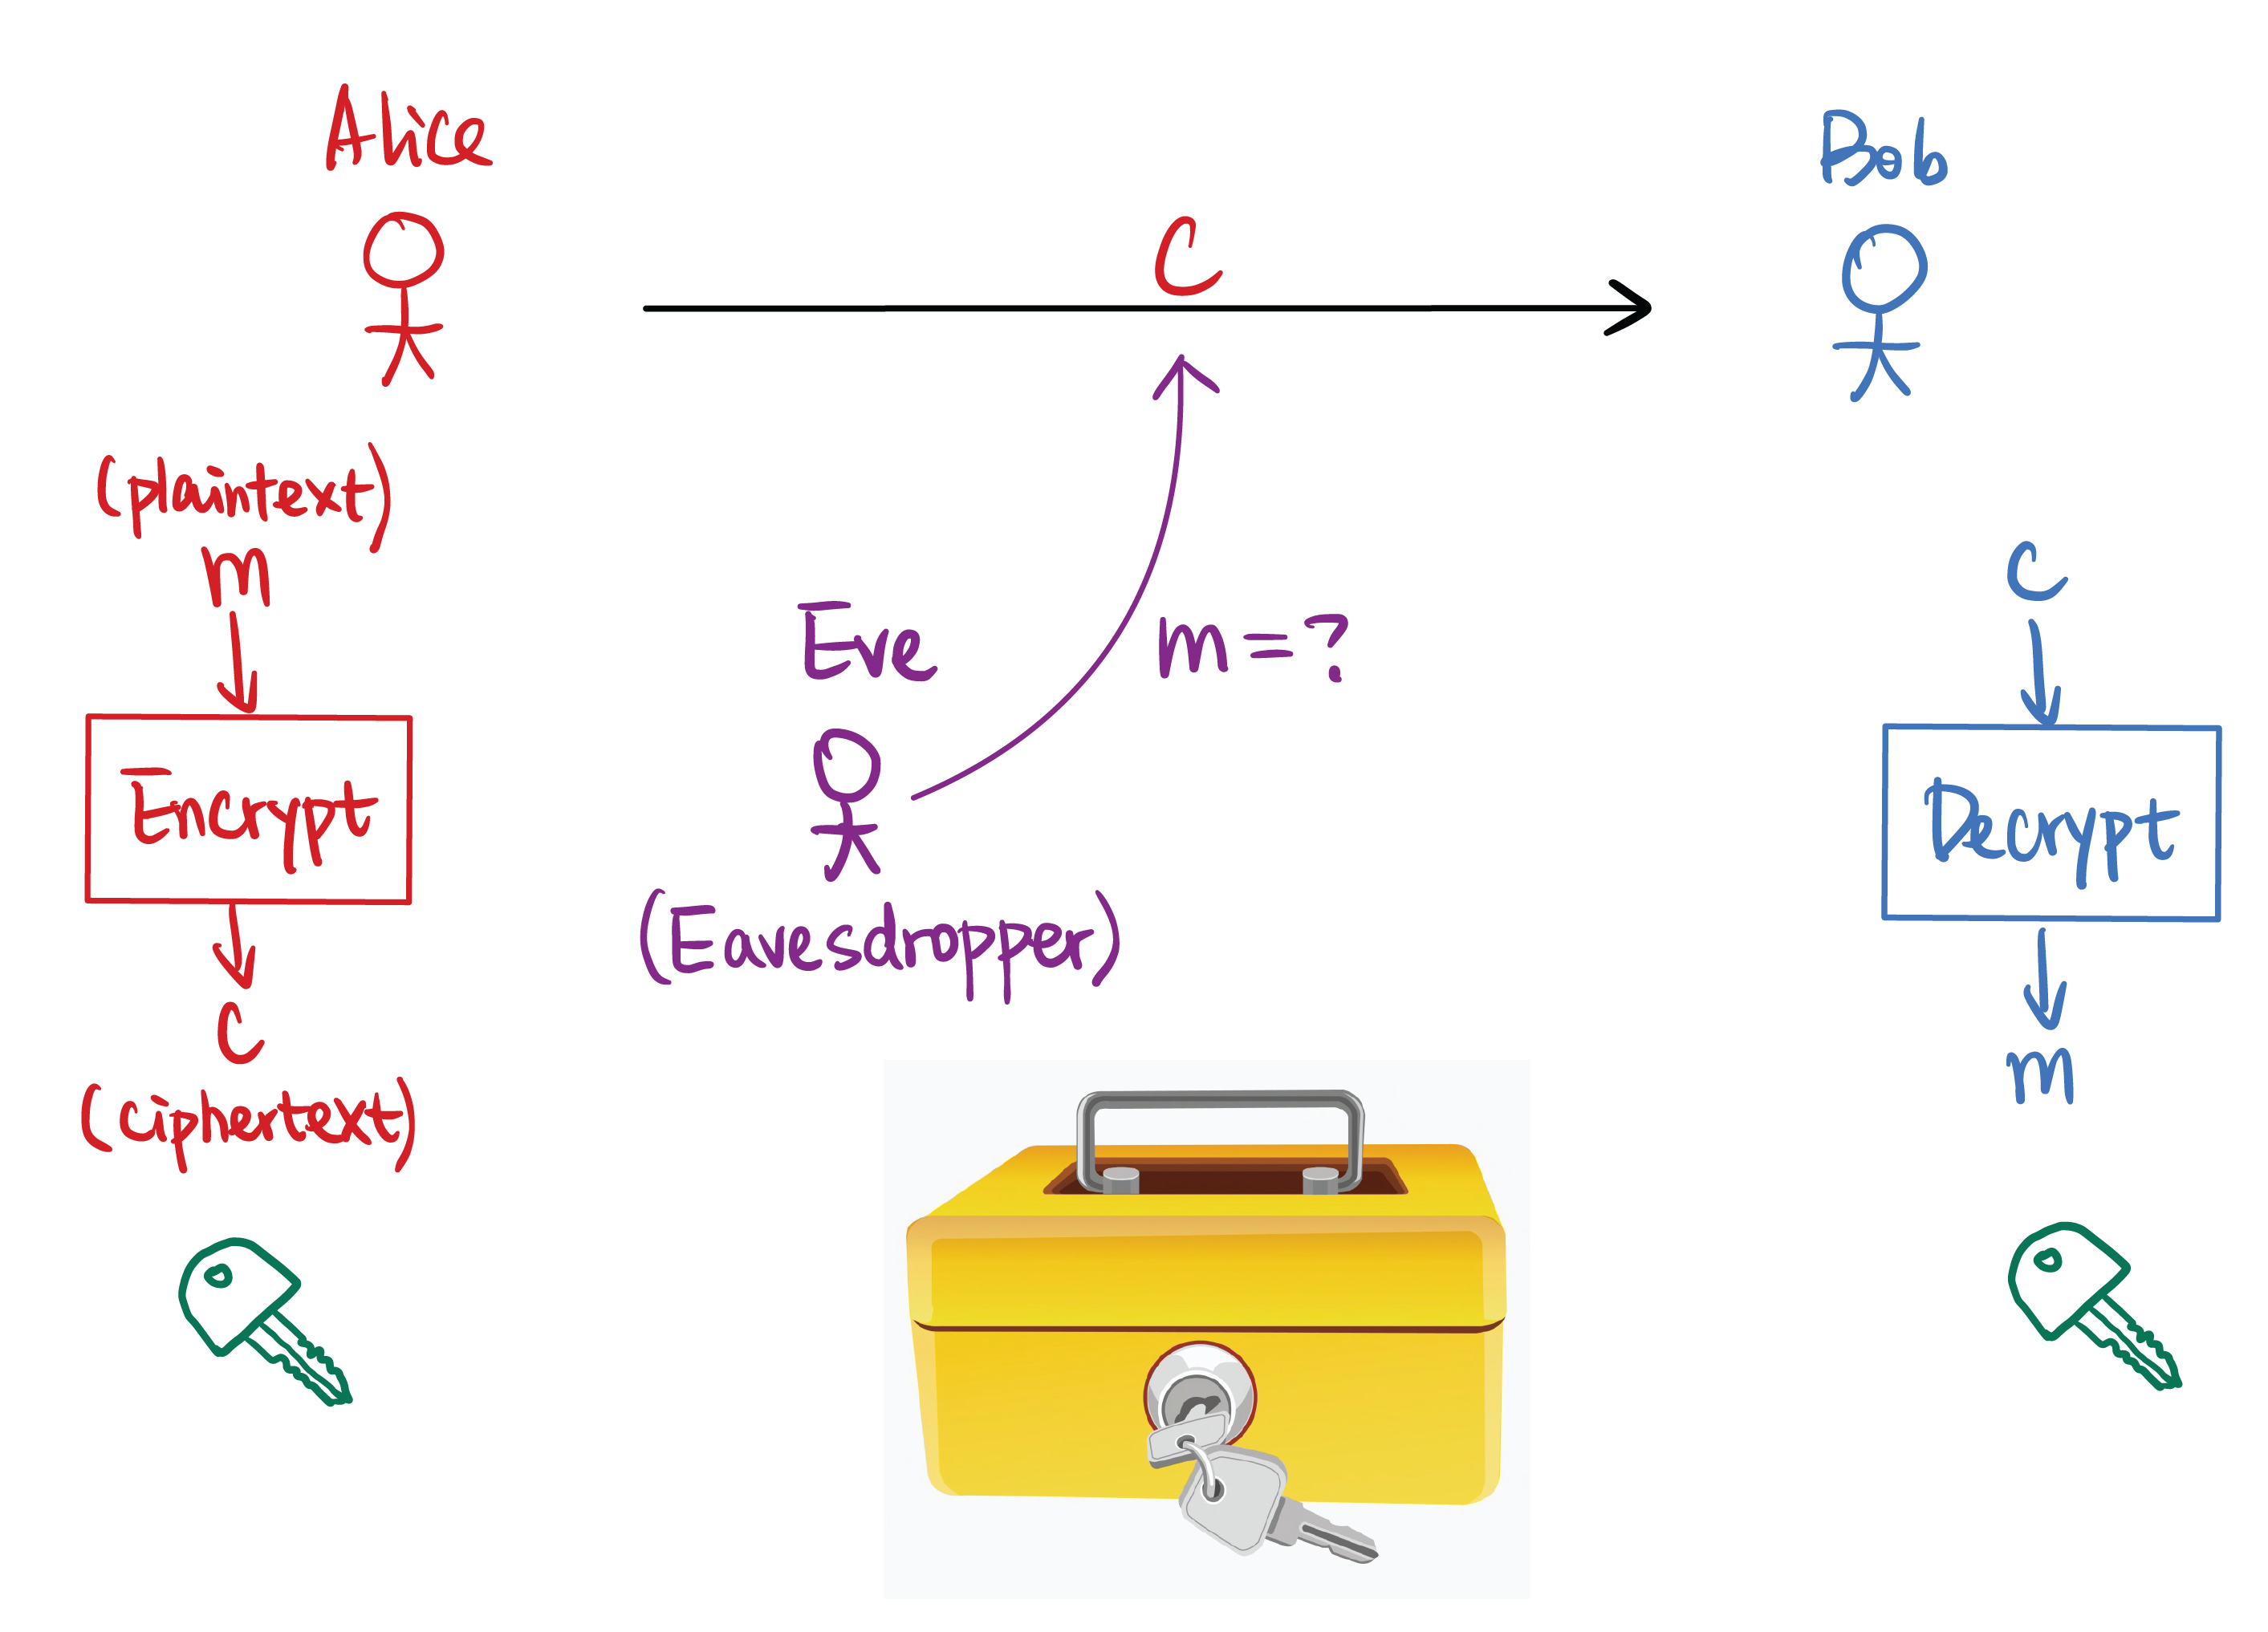
\includegraphics[width=0.8\textwidth]{images/2023-01-26/message_secrecy.png}
    \end{center}

    In this model, Eve is a weaker adversary, an \emph{eavesdropper}. Eve can only see the message, not alter it.
\end{definition}

\begin{example}[Substitution Cipher]
    The key that Alice and Bob jointly uses is a permutation mapping from $\{A\dots Z\}\to \{A\dots Z\}$. This mapping is the \emph{secret key}.

    Bob also has the mapping, and takes the inverse of the permutation to retrieve the message.

    \begin{center}
        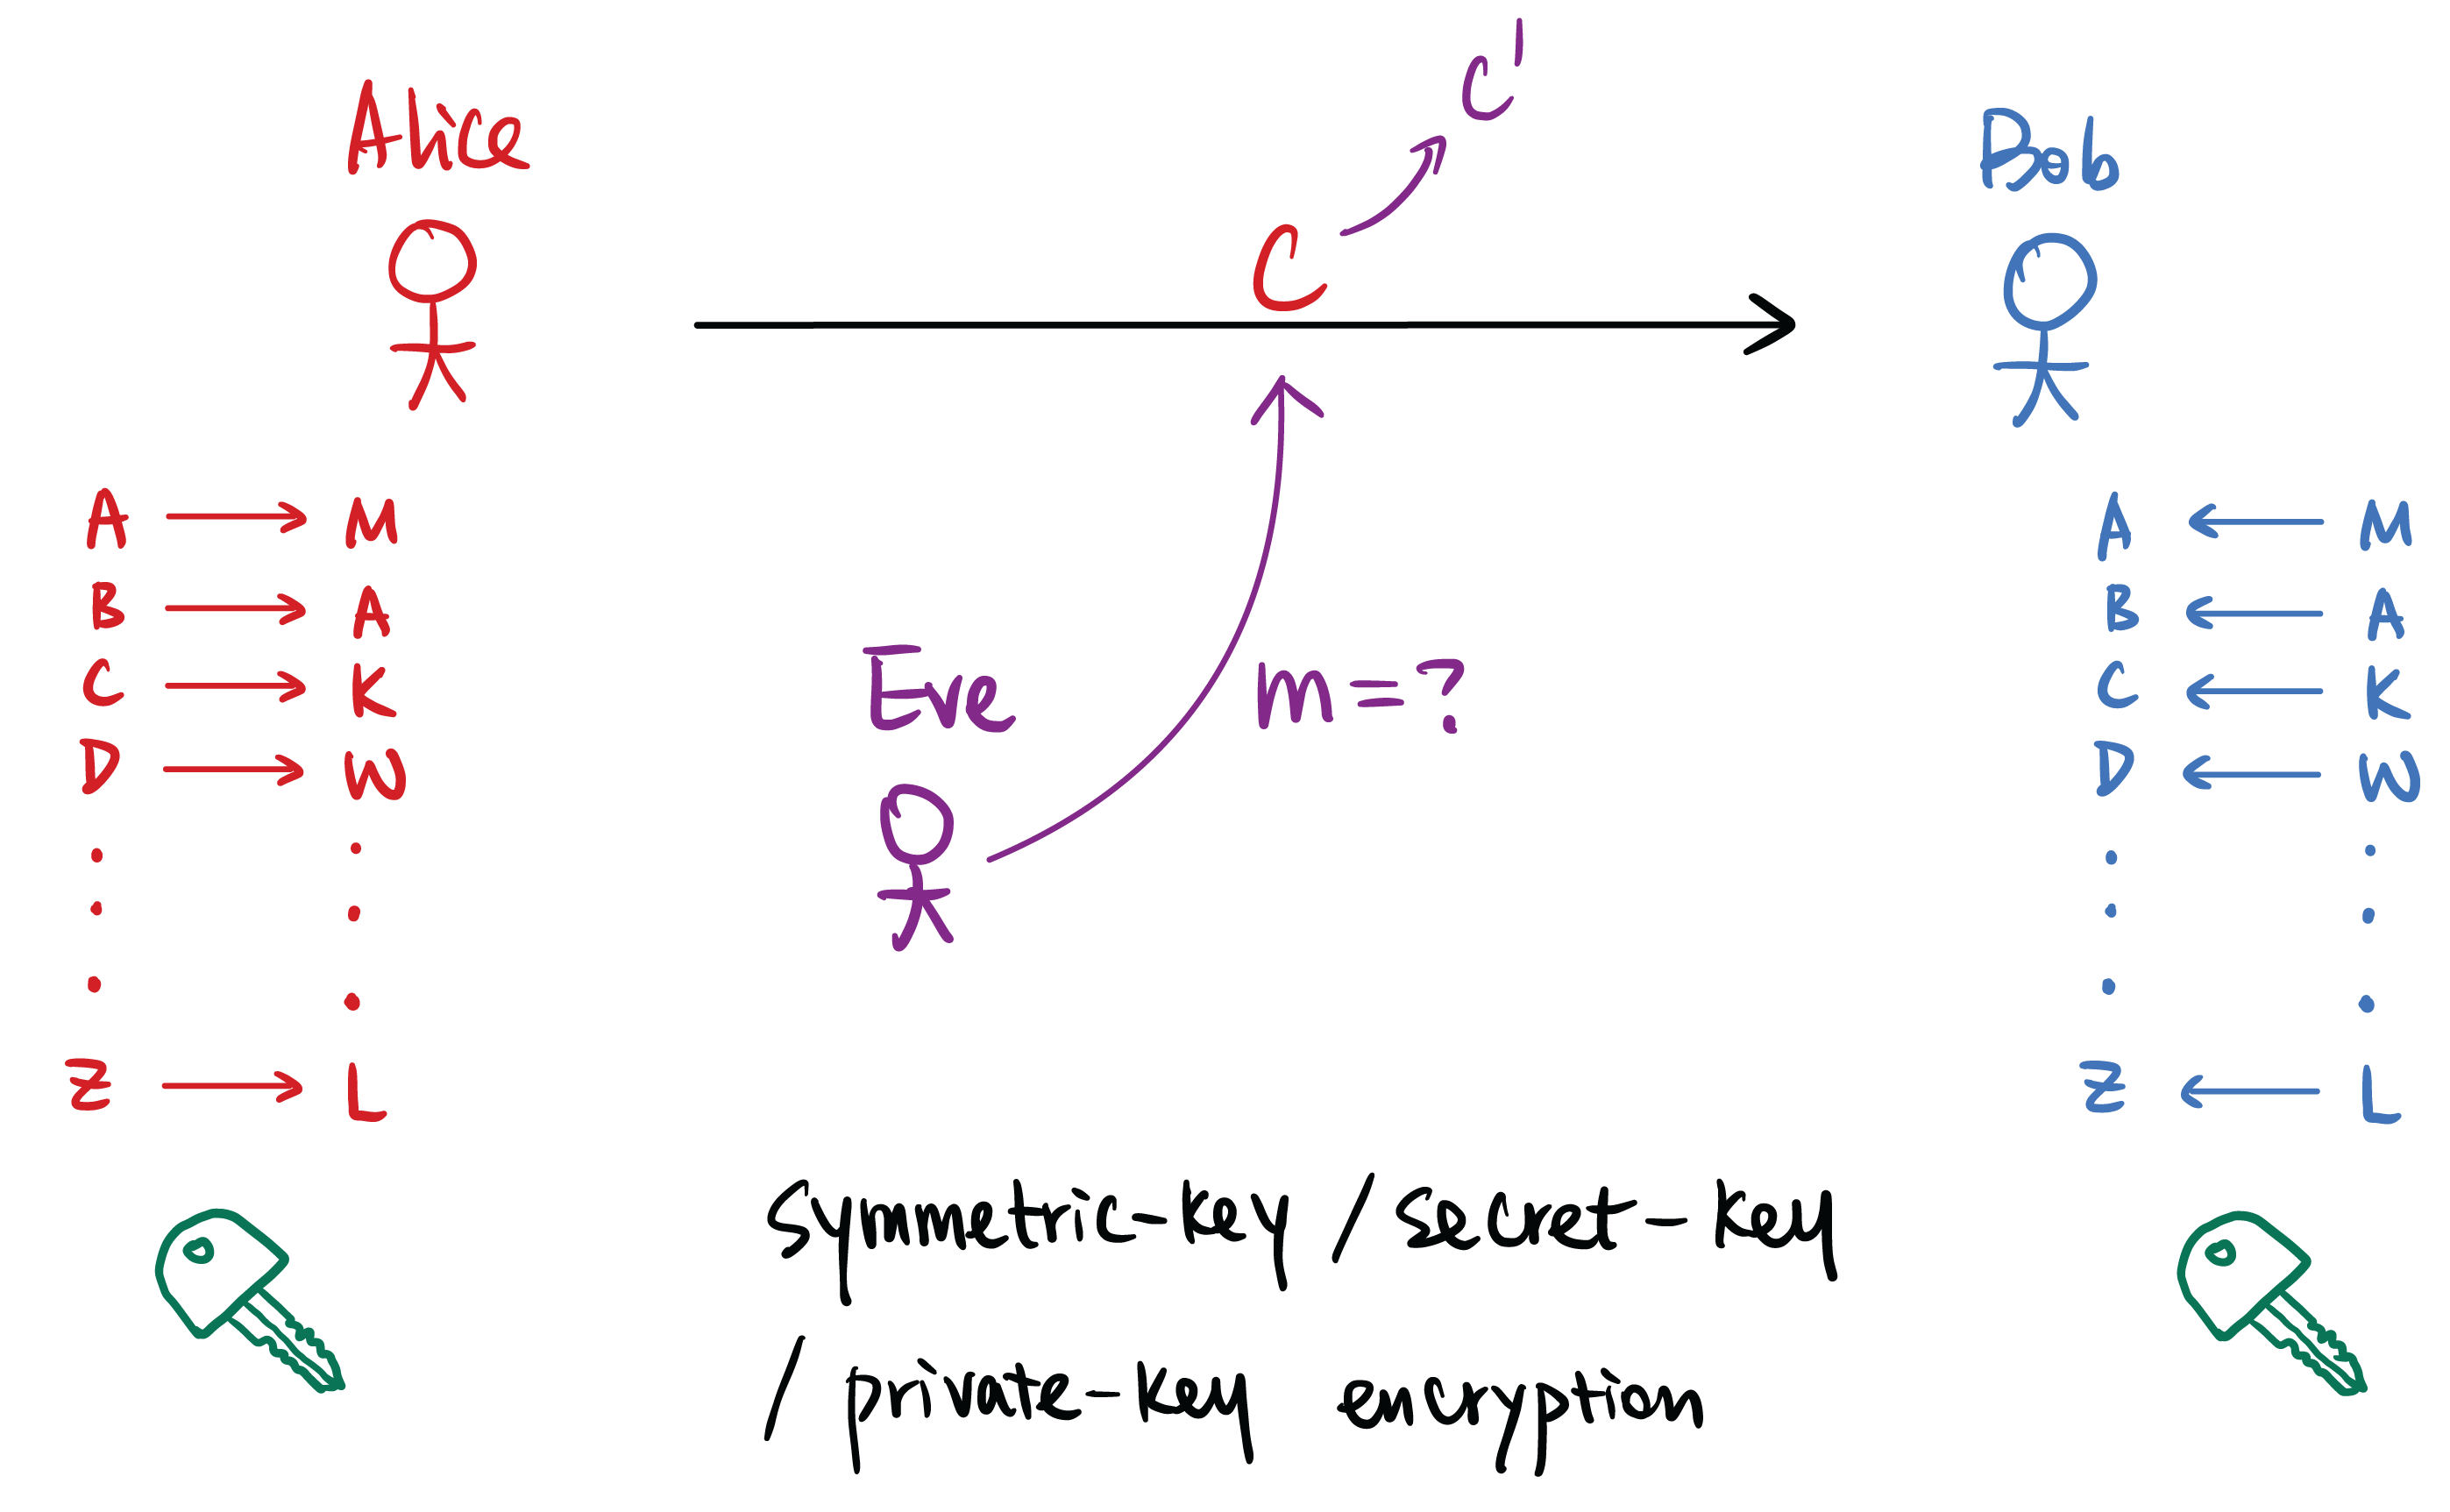
\includegraphics[width=0.9\textwidth]{images/2023-01-26/substitution_cipher.png}
    \end{center}

    This scheme is not quite secure! \emph{Why?}

    Given a large enough text, you can apply frequency analysis and break the substitution cipher.
\end{example}
\begin{remark*}
    This encryption scheme also requires that Alice and Bob meet up in person to exchange this shared private key. Schemes like this are called \emph{symmetric-key, secret-key, or private-key encryption}. They need to somehow agree first on the same secret key.
\end{remark*}

\begin{definition}[Public-key Encryption]
    There is another primitive that is much stronger: \ul{public-key encryption}. Bob publishes both a \emph{public} key and a \emph{private} key. You can consider a lock where you don't need a key to lock it\framedfootnote{You literally click it closed}, and only Bob has the key to unlock it.

    \begin{center}
        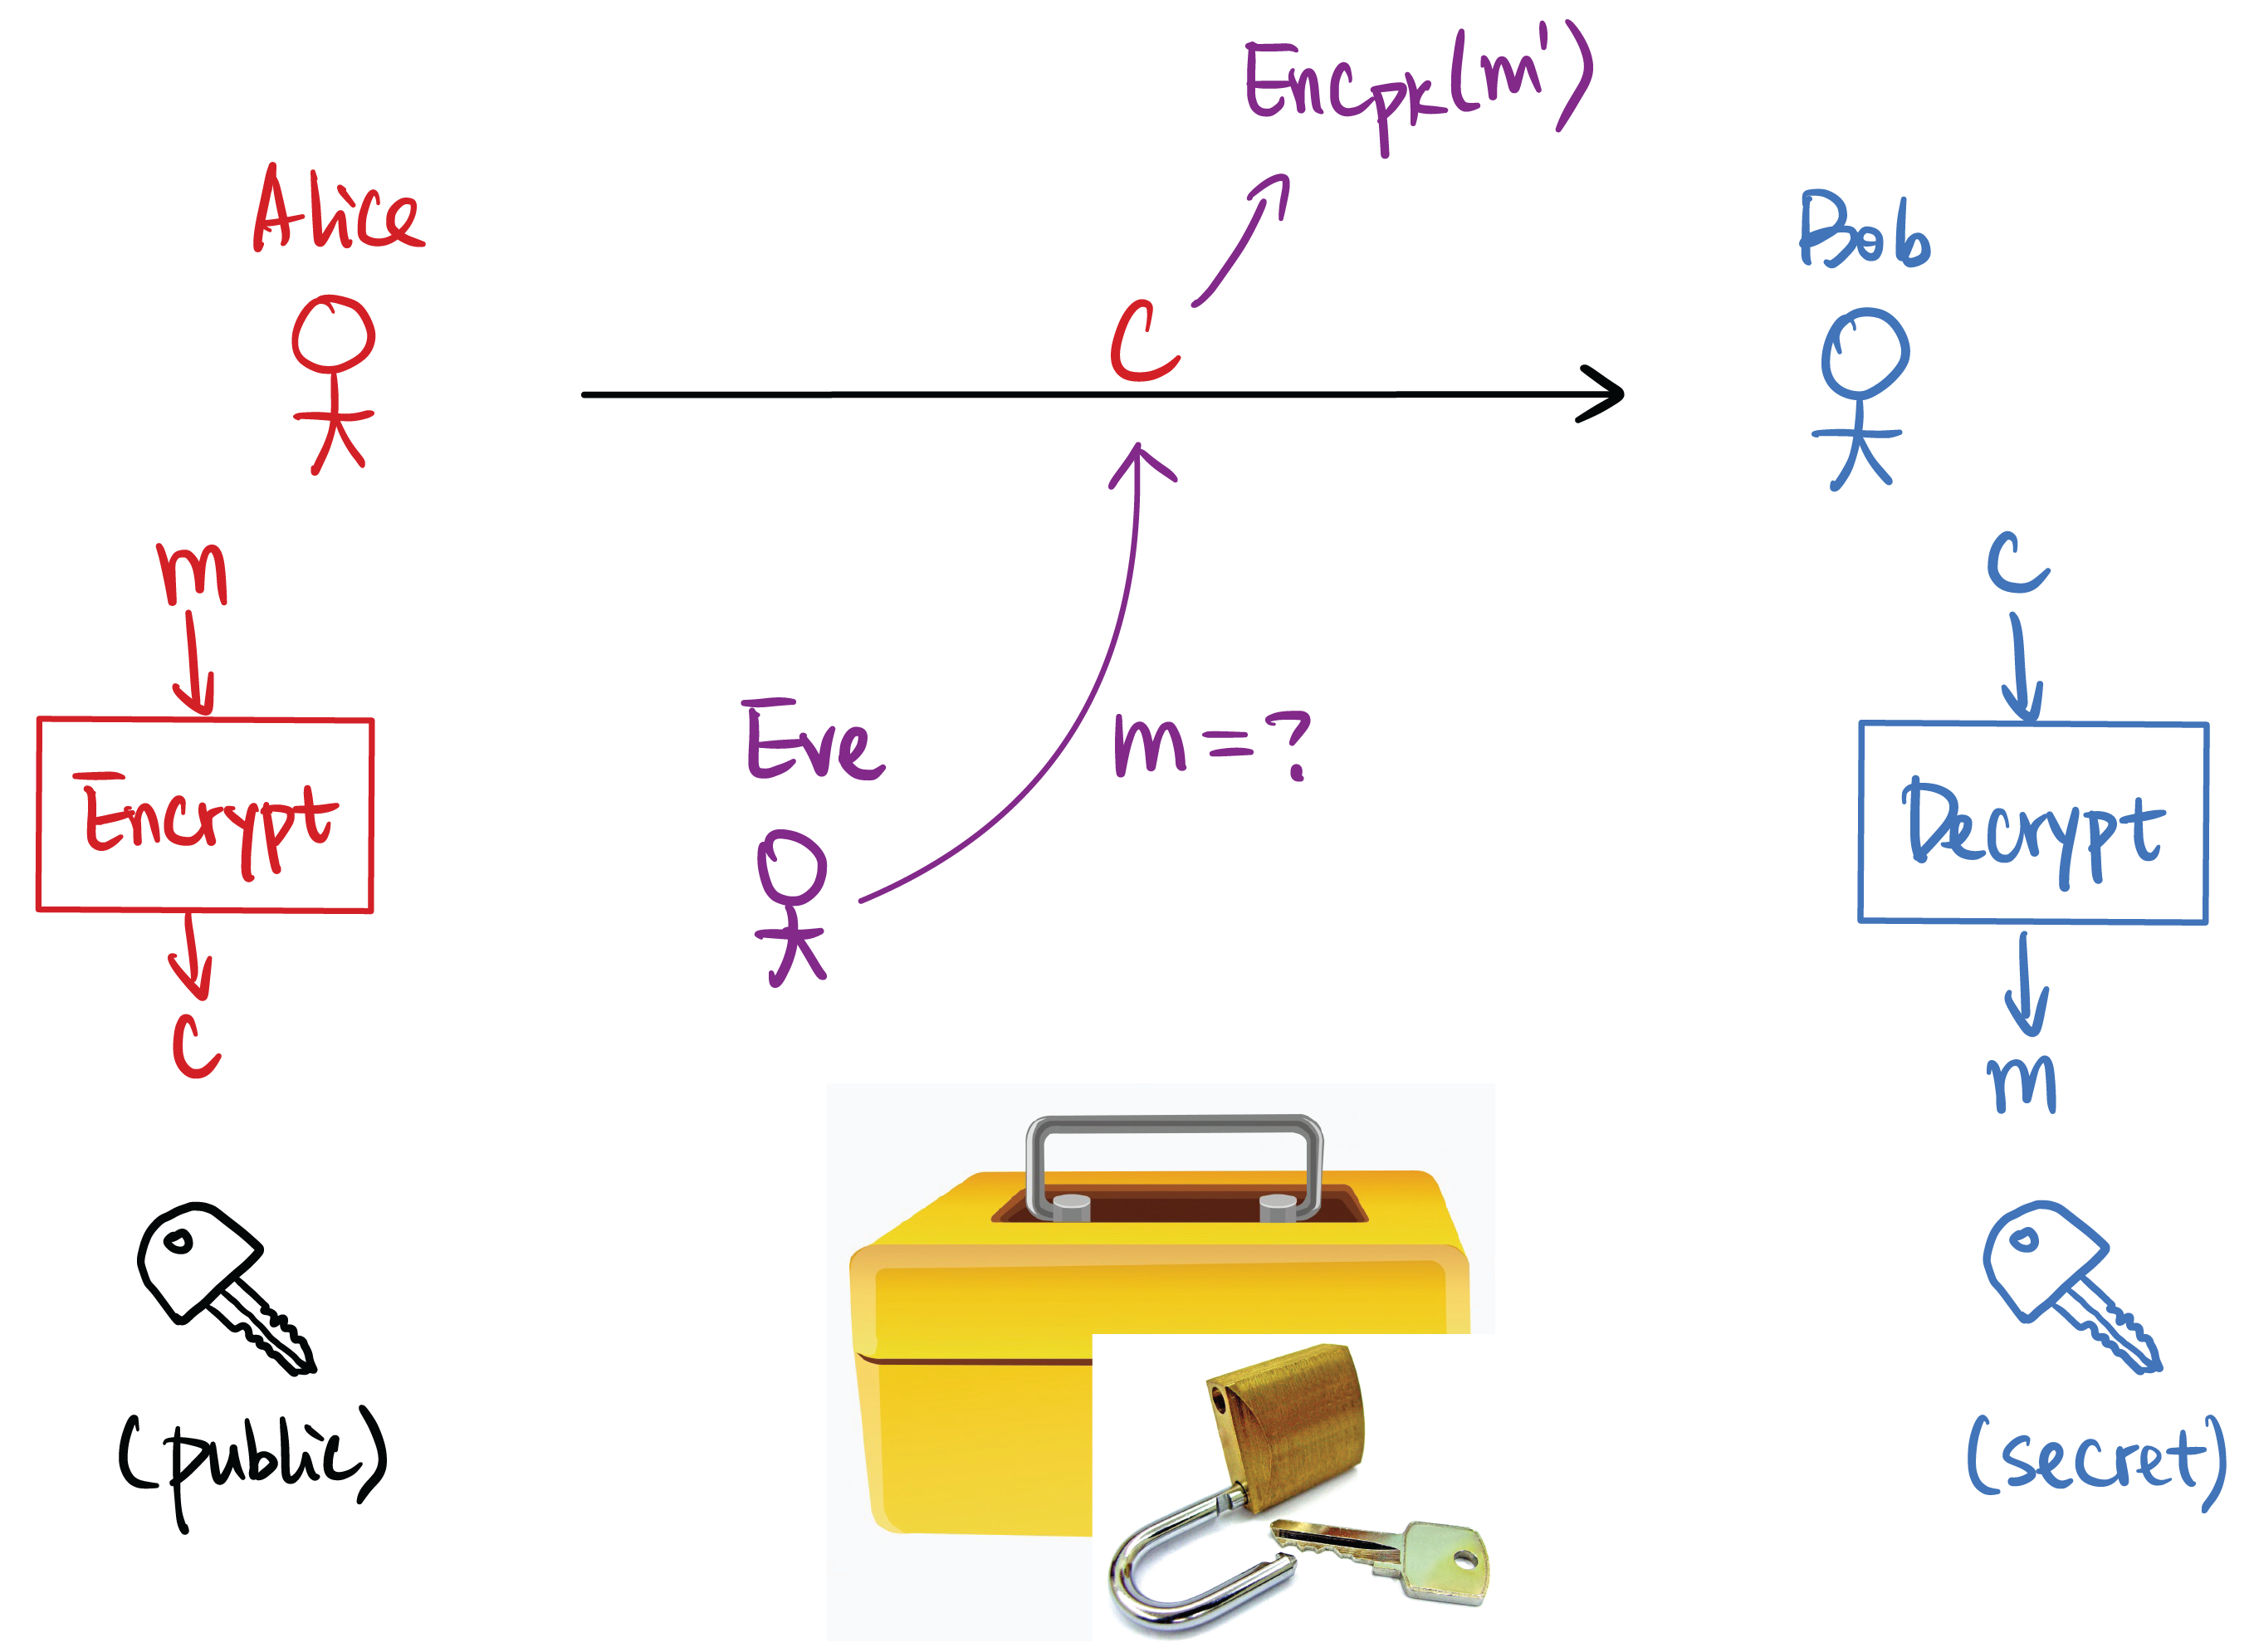
\includegraphics[width=0.9\textwidth]{images/2023-01-26/public_key.png}
    \end{center}

    This is seemingly magic! Bob could publish a public key on his homepage, anyone can encrypt using a public key but only Bob can decrypt. \emph{Stay tuned, we will see public-key encryption schemes next lecture!}
\end{definition}

\subsubsection{Message Integrity}
Alice wants to send a message to Bob again, but Eve is stronger! Eve can now tamper with the message.

\begin{center}
    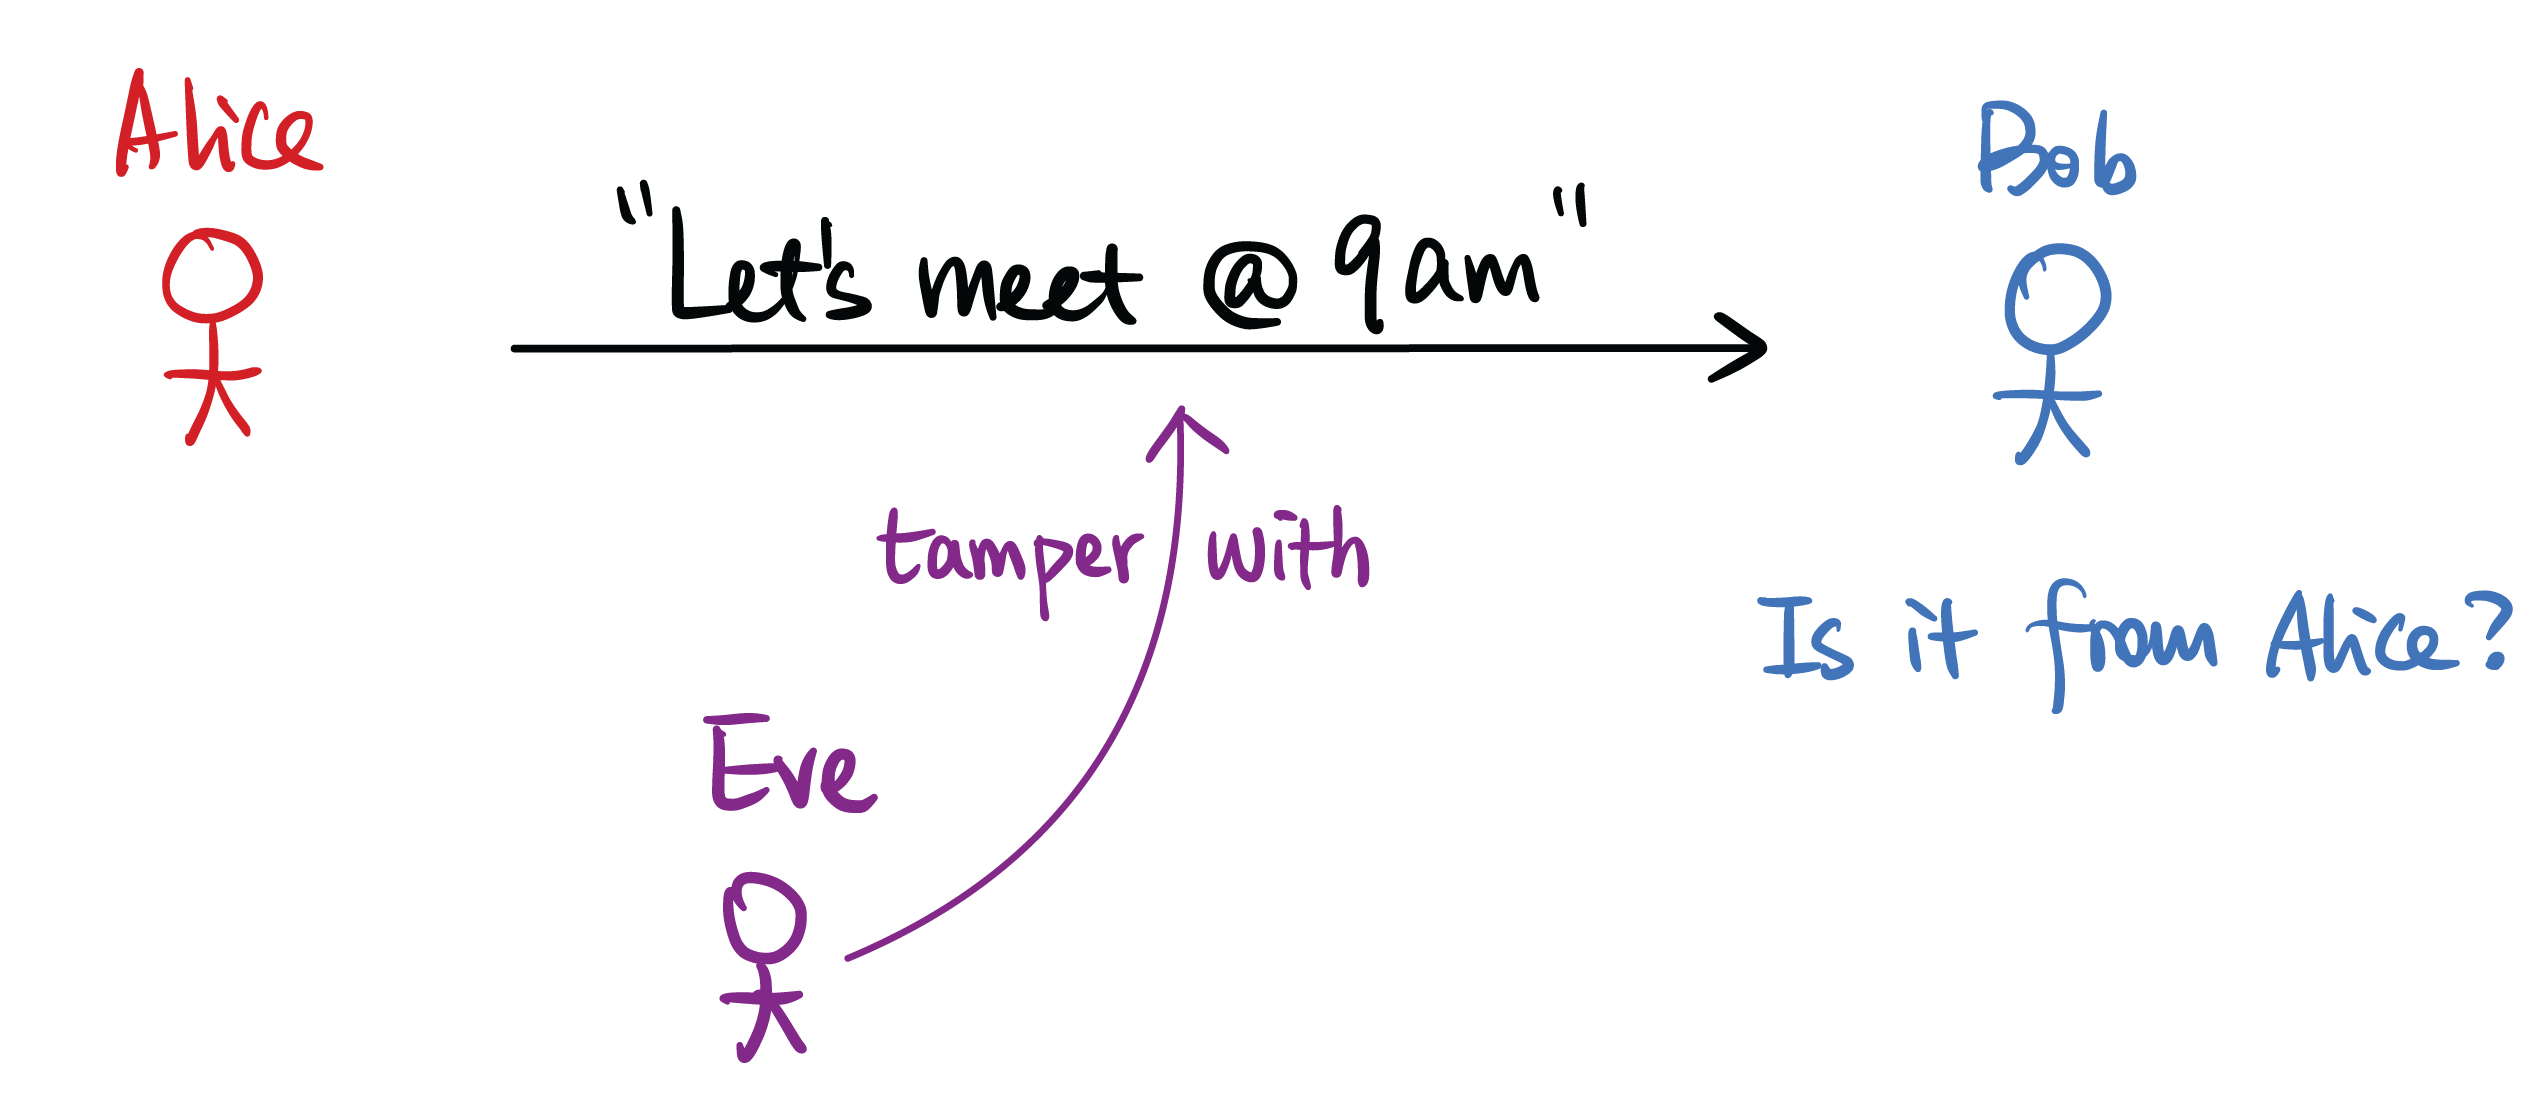
\includegraphics[width=0.9\textwidth]{images/2023-01-26/integrity.png}
\end{center}

Bob wants to ensure that the message \emph{actually} comes from Alice. Does our previous scheme (of encrypting messages) solve this problem? Nope!

Eve can change the ciphertext to something else, they could pretend to be Alice. In secret-key schemes, if Eve figures out the secret-key, they can forge messages from Alice. Even if Eve doesn't know the underlying message, they could still change it to some other ciphertext which might be correlated to the original ciphertext, \emph{without knowing the underlying message}. We'll see how Eve can meaningfully do this in some schemes. Alice could send a message ``Let's meet at $x$ AM'' and Eve could tamper this to say ``Let's meet at $x+1$ AM.''

This is sort of an orthogonal problem to message secrecy. For example, when Alice logs in to Google, Google needs to verify that Alice actually is who she claims to be.

\begin{center}
    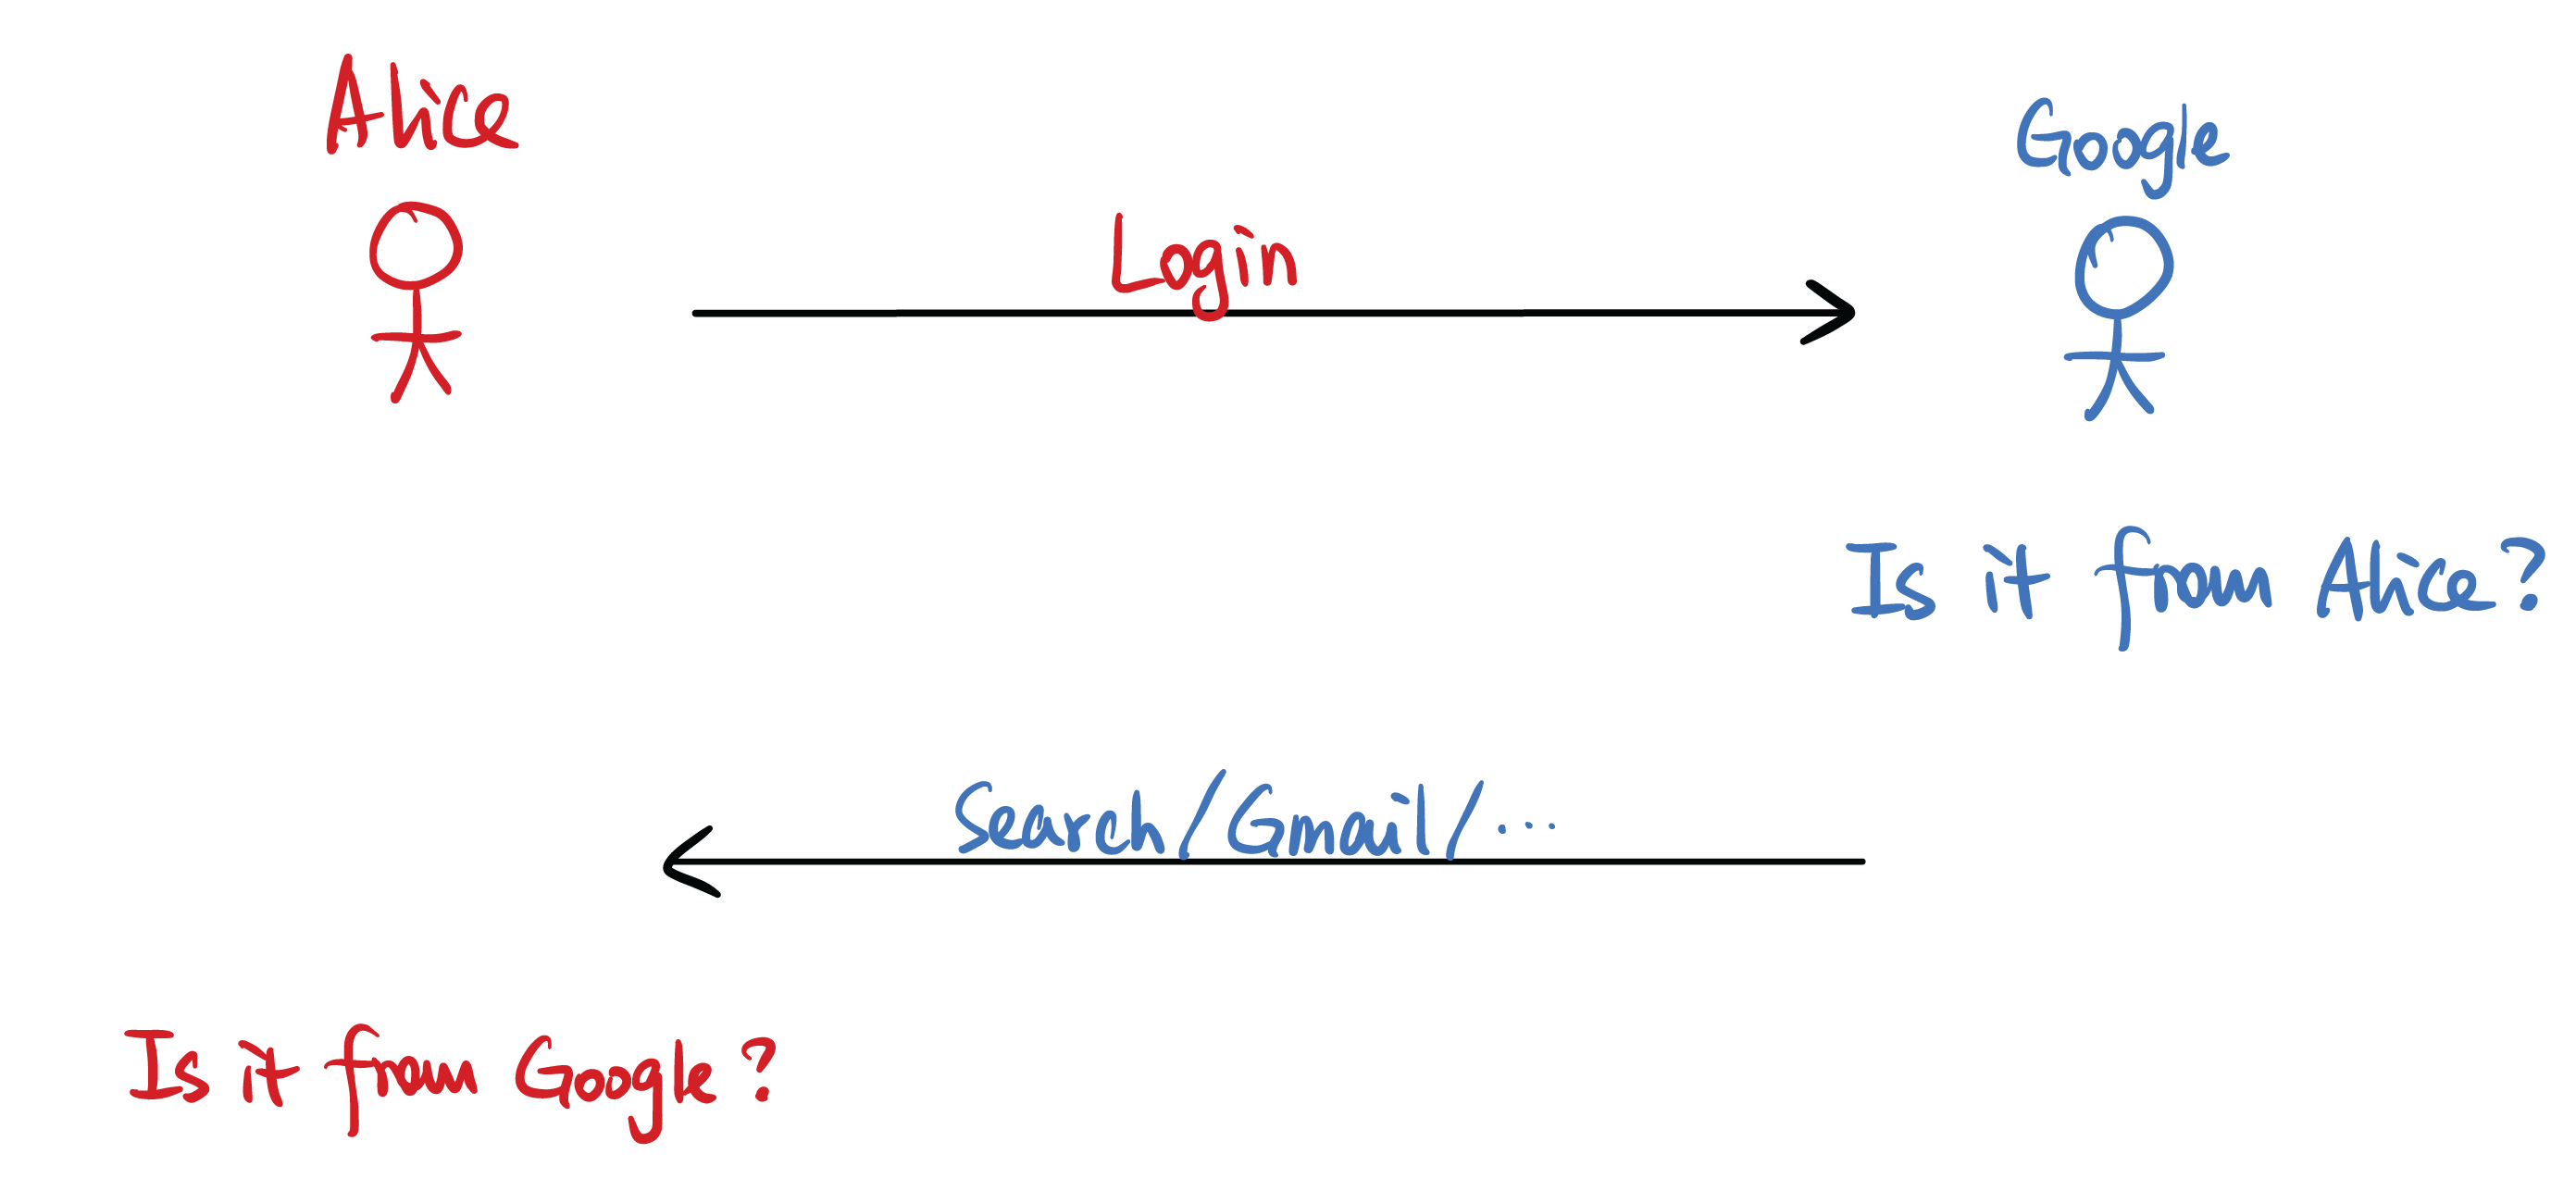
\includegraphics[width=0.9\textwidth]{images/2023-01-26/authentication.png}
\end{center}

This property that we want is called \ul{message integrity}.

\subsubsection{Signal and Auth}

The first two projects are Signal and Auth whose aim will be to cover \ul{secure messaging} and \ul{secure authentication}.

\emph{Projects Overview}
\begin{enumerate}
    \setcounter{enumi}{-1}
    \item Warm-up, you will implement some basic cryptographic schemes.
    \item Secure Communication: how to communicate in secret.
    \item Secure Authentication: how to authenticate yourself.
    \item Zero-Knowledge Proofs: we'll use ZKPs to implement a secure voting scheme.
    \item Secure Multiparty Computation: we'll implement a way to run any function securely between two parties.
    \item Fully Homomorphic Encryption: a form of post-quantum cryptography.
\end{enumerate}

We'll now introduce the latter three projects!

\subsection{Zero-Knowledge Proofs}
This is to prove something without \emph{revealing} any additional knowledge.

For example, Alice may want to
\begin{itemize}
    \item Prove she knows the difference in taste between Coke and Pepsi without revealing how
    \item Prove that you have a bug in your code without revealing the bug
    \item She has the secret key for this ciphertext without revealing the plaintext
\end{itemize}

How is this possible?
\begin{example*}
    Alice claims to be able to differentiate between Coca-Cola and Pepsi! She wants to prove this to Bob without revealing her secrets.

    Bob will randomly sample a bit $b\overset{\$}{\leftarrow}\{0, 1\}$, with $b=0$ being Coca-Cola and $b=1$ being Pepsi. Bob will let Alice taste this drink. Alice will give a guess $b'$ of what drink it is.

    \begin{center}
        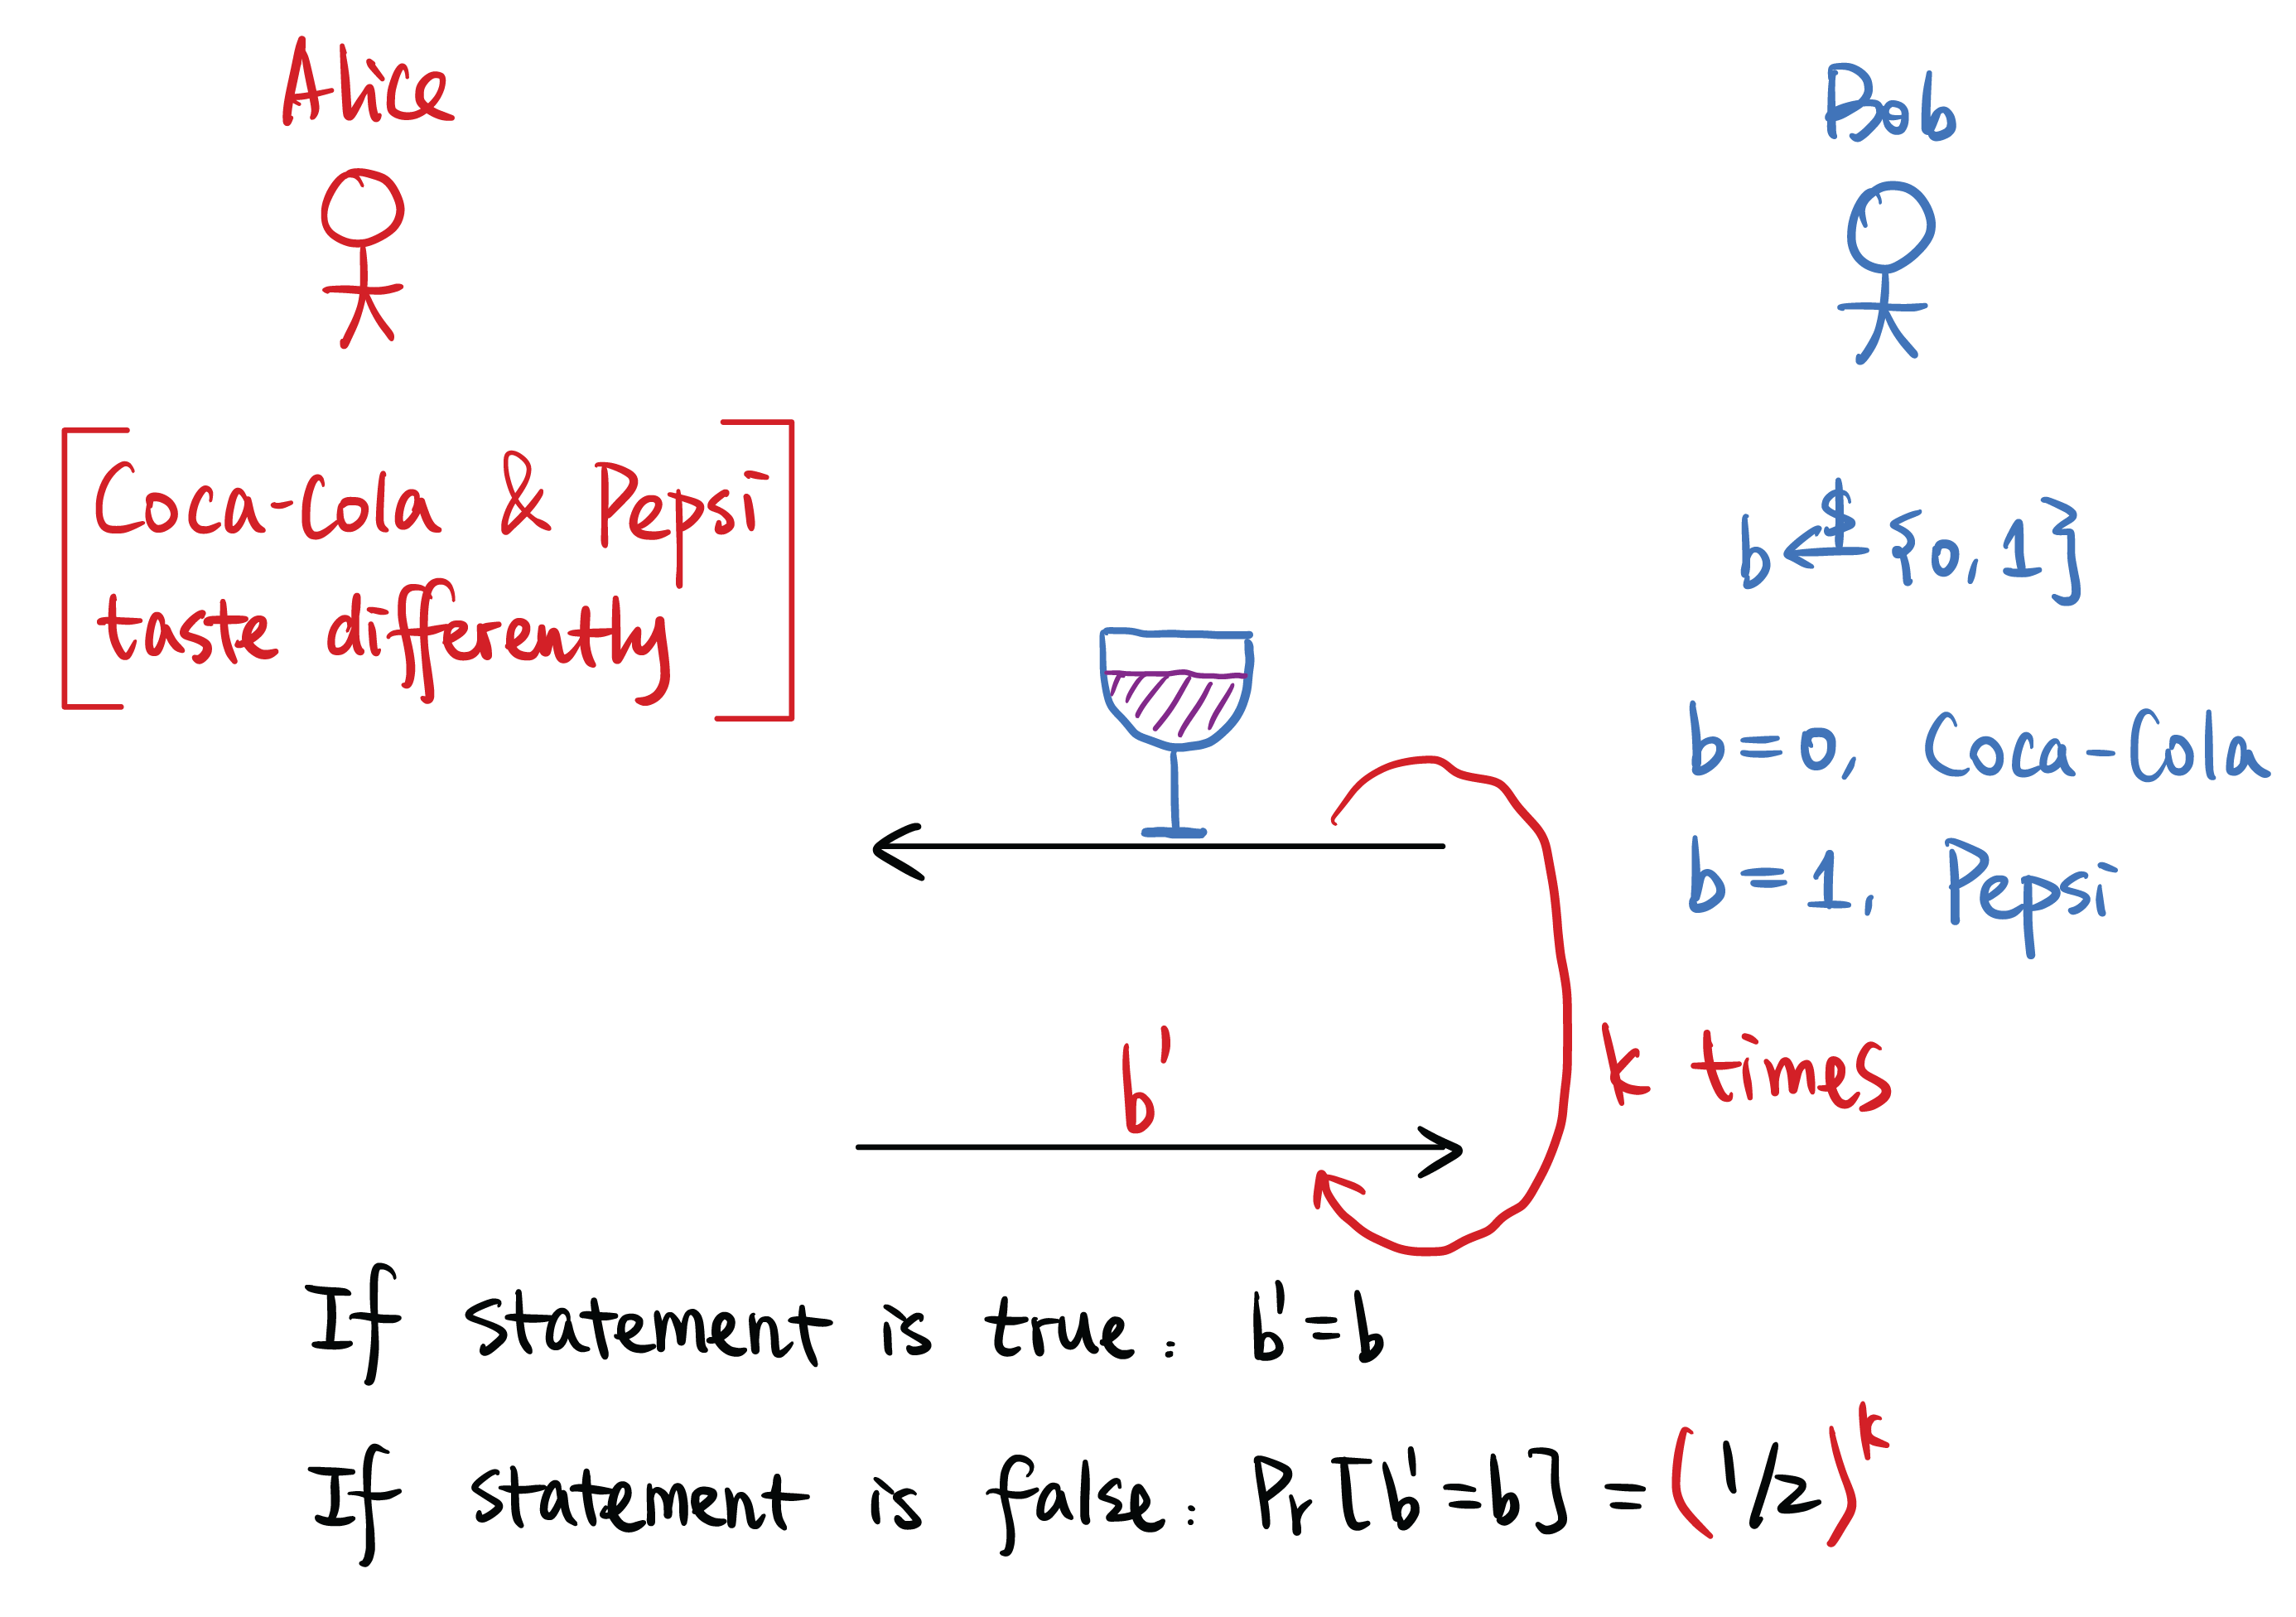
\includegraphics[width=0.9\textwidth]{images/2023-01-26/zk_cola.png}
    \end{center}

    If the statement is true, $\Pr[b' = b] = 1$ (Alice always gives the correct prediction).

    If the statement is false, $\Pr[b' = b] = \frac{1}{2}$ (Alice is guessing with $0.5$ probability).

    To enhance this, we can run this a total of $k$ times. If we run it enough times, Bob will be more and more confident in believing this. Alice getting this correct by chance has a $\frac{1}{2^k}$ probability.

    The key idea, however, is that Bob doesn't gain any knowledge of how Alice differentiates.

    \begin{remark*}
        This is a similar strategy in proving graph non-isomorphism.

        For people who have seen this before, generally speaking, any $\textsf{NP}$ language can be proved in zero-knowledge. Alice has the \emph{witness} to the membership in $\textsf{NP}$ language.
    \end{remark*}
\end{example*}

\subsection{Secure Multi-Party Computation}
\begin{center}
    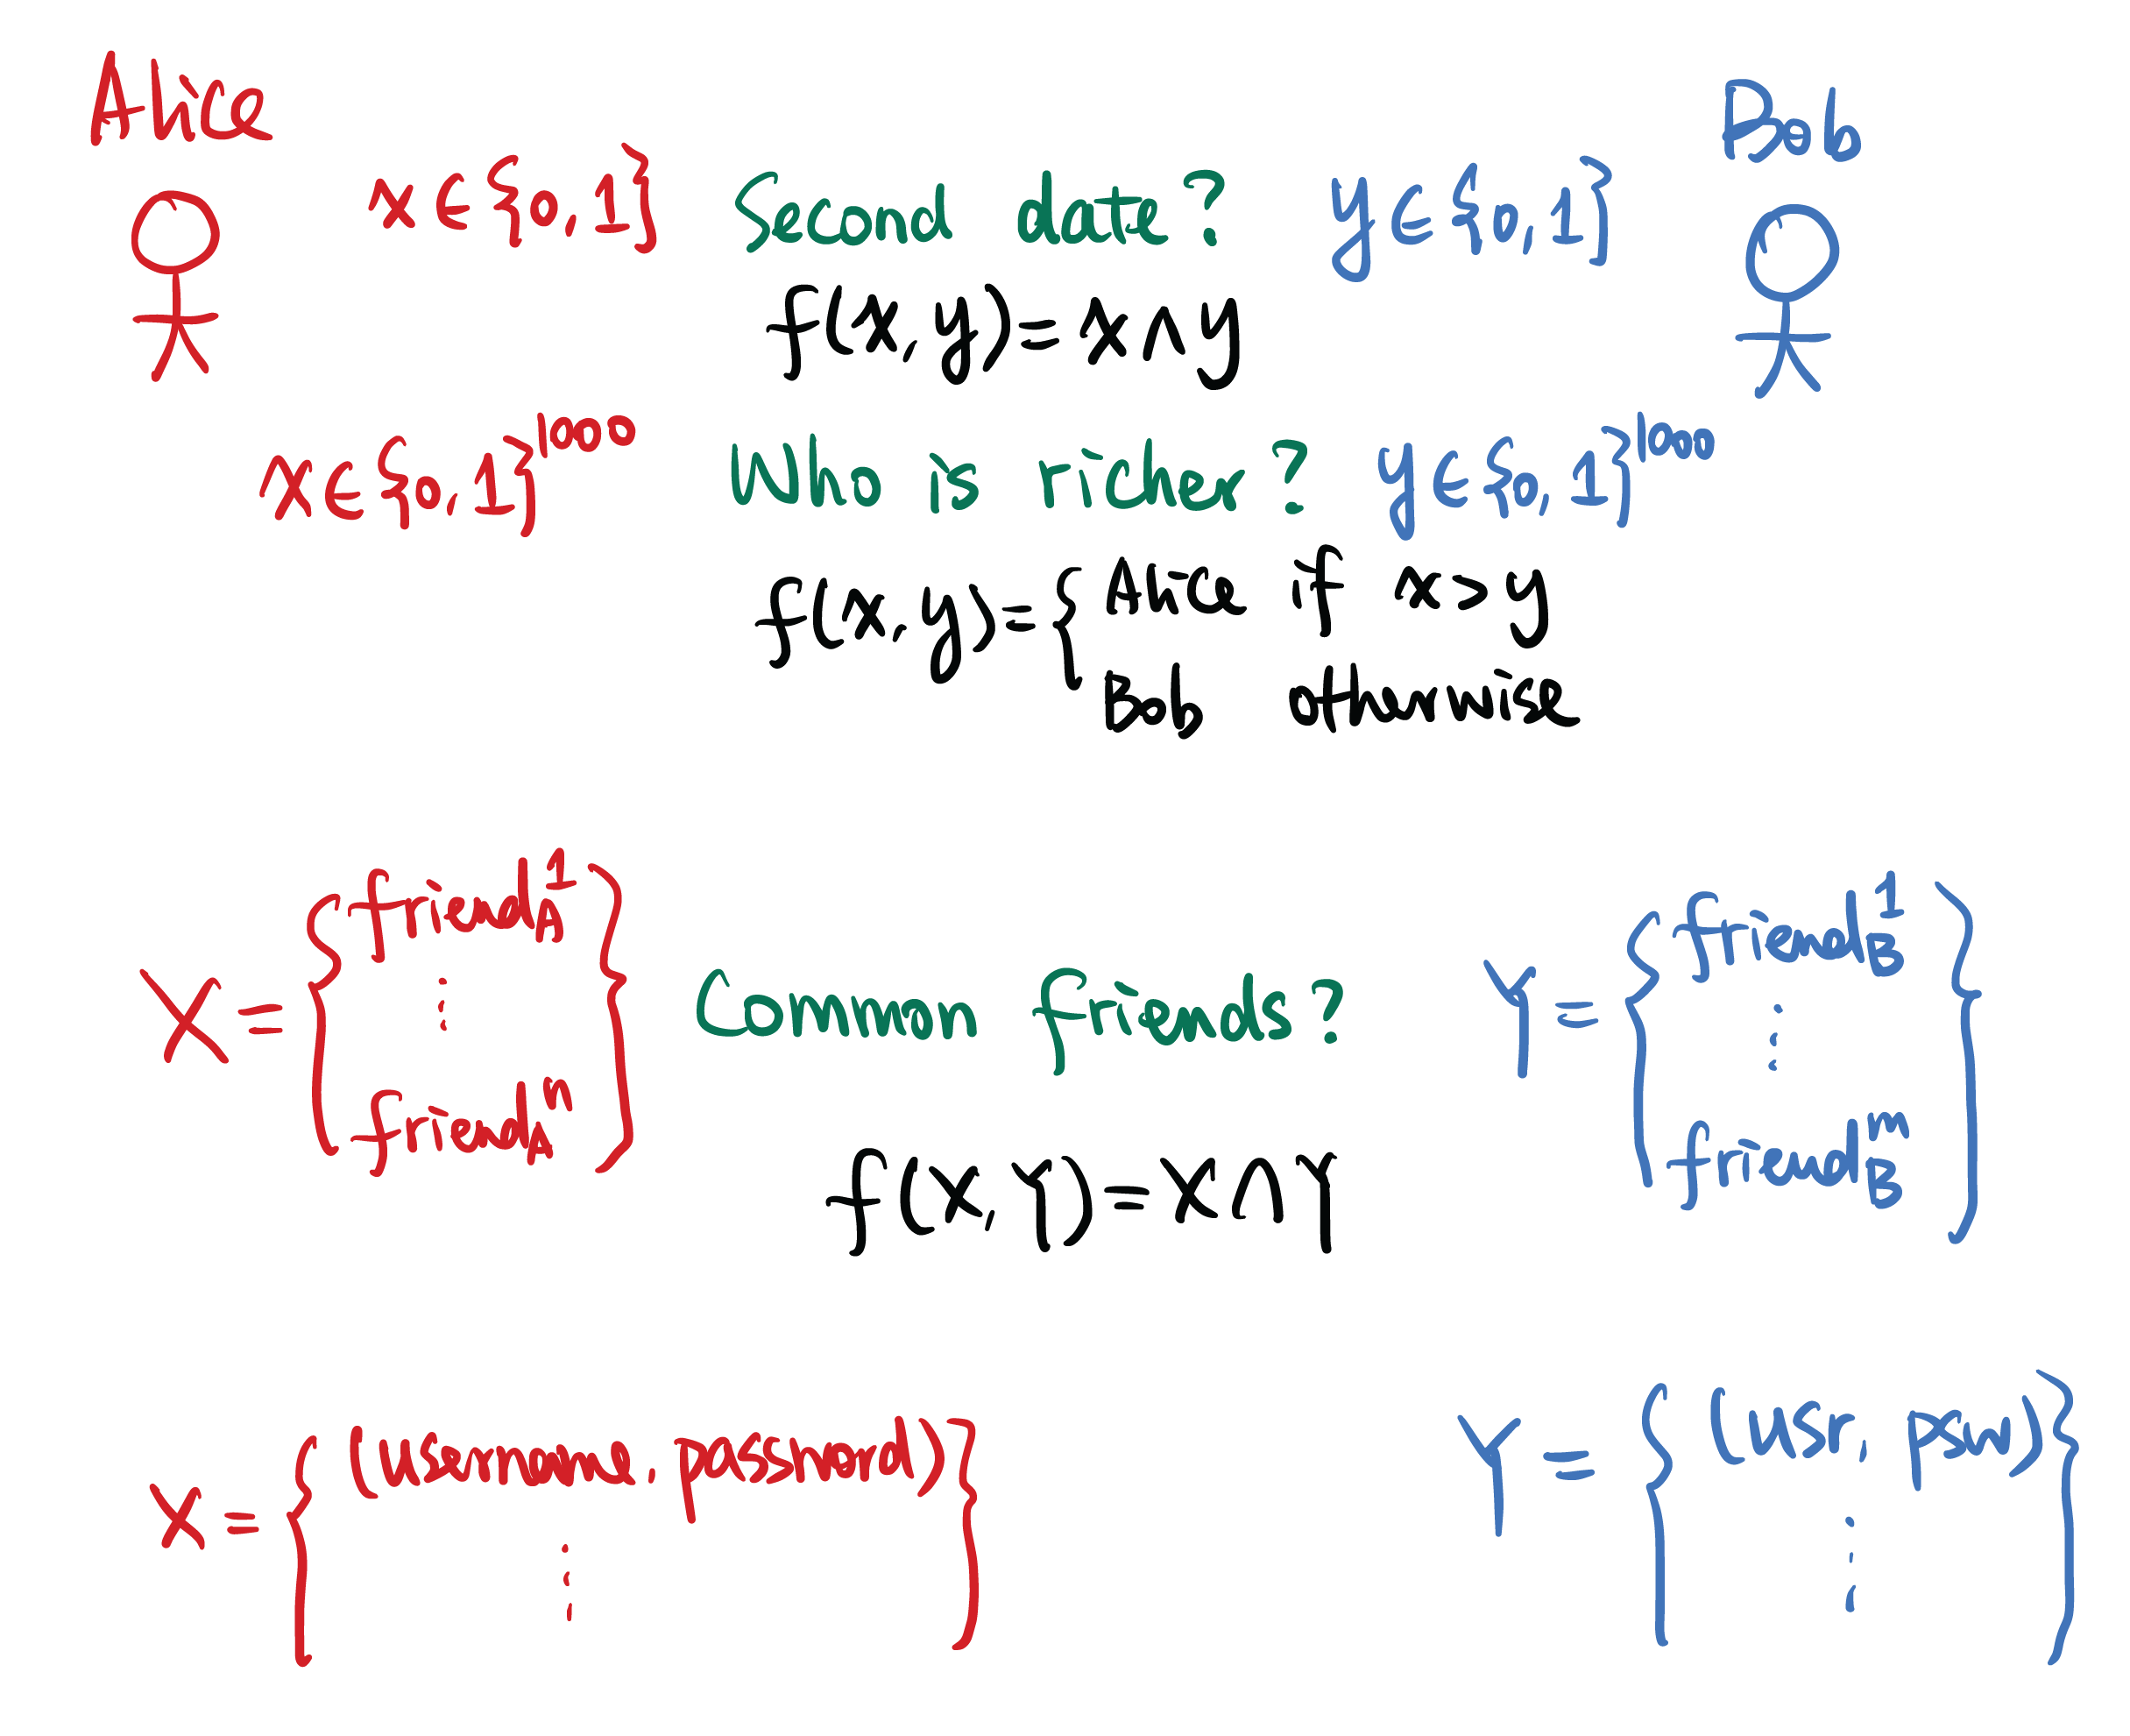
\includegraphics[width=0.9\textwidth]{images/2023-01-26/secure_mpc.png}
\end{center}

\begin{example*}[Secure \textsf{AND}]
    Alice and Bob go on a first date, and they want to figure out whether they want to go on a second date. They will only go on a second date if and only if both agree to a second date.

    How will they agree on this? They could tell each other, but this could be embarrassing. One way is for them to share with a third-party (this is what dating apps do!). However, there might not always be an appropriate third party (in healthcare examples, not everyone can be trusted with the data).

    In this case, Alice has a choice bit $x\in\{0, 1\}$ and Bob has a choice bit $y\in\{0, 1\}$. They are trying to jointly compute $f(x, y) = x\land y$.

    \begin{remark}
        Couldn't a party still figure out how the other party feels? For example, if Bob's bit was 1 and the joint result was 0, Bob can \emph{infer} that Alice's bit was 0.

        This is, in effect, the best we can do. The ideal guarantee is that each party only learns any information they can infer from the \emph{output} and their input. However, they should not learn anything more.
    \end{remark}
\end{example*}

What are we trying to achieve here? We want to jointly compute some function, where each party has private input, such that each party only learns the output. They should not learn anything about other partys' inputs.

\begin{example*}[Yao's Millionaires' Problem]
    Perhaps, Alice and Bob wants to figure out who is richer. The inputs are $x\in\{0, 1\}^{1000}$ and $y\in\{0, 1\}^{1000}$ (for simplification, let's say they can express their wealth in 1000 bits). The output is the person who has the max.
    \[f(x, y) = \begin{cases}
            \text{Alice} & \text{if }x > y  \\
            \text{Bob}   & \text{otherwise}
        \end{cases}\]
\end{example*}

\begin{example*}[Private Set Intersection]\label{ex:psi}
    Alice and Bob meet for the first time and want to determine which of their friends they share. However, they do not want to reveal who specifically are their friends.

    $X$ is a set of A's friends $X = \{\mathsf{friend}_A^1, \mathsf{friend}_A^2, \cdots, \mathsf{friend}_A^n\}$ and Bob also has a set $Y = \{\mathsf{friend}_B^1, \mathsf{friend}_B^2, \cdots, \mathsf{friend}_B^m\}$. They want to jointly compute \[f(X, Y) = X\cap Y.\]

    You might need to reveal the cardinality of these sets, but you could also pad them up to a maximum number of friends.

    This has a lot of applications in practice! In Google Chrome, your browser will notify you that your password has been leaked on the internet, without having access to your passwords in the clear. $X$ will be a set of \emph{your} passwords, and Google will have a set $Y$ of \emph{leaked} passwords. The \emph{intersection} of these sets are which passwords have been leaked over the internet, without revealing all passwords in the clear.
\end{example*}
\begin{ques*}
    Isn't the assumption that the size of input records is revealed weaker than using a trusted third-party?

    Yes, however in some cases (hospital health records), parties are legally obliged to keep data secure. We wish for security more than the secrecy of cardinality.
\end{ques*}

In the general case, Alice and Bob have some inputs $x$ and $y$ with bounded length, and they want to jointly compute some function $f$ on these inputs. This is \ul{Secure Two-Party Computation}. Furthermore, there could be multiple parties $x_1, \dots, x_n$ that jointly compute $f(x_1, \dots, x_n)$ that hides each input. This is \ul{Secure Multiparty Computation}.

We'll explore a toy example with the bit-\textsf{AND} from the dating example.

\begin{example*}[Private Dating]
    Alice and Bob have choice bits $x\in\{0, 1\}$ and $y\in\{0, 1\}$ respectively. There is a \emph{physical} round table with $5$ identical slots, one already filled in with a $1$ facing down.

    \begin{center}
        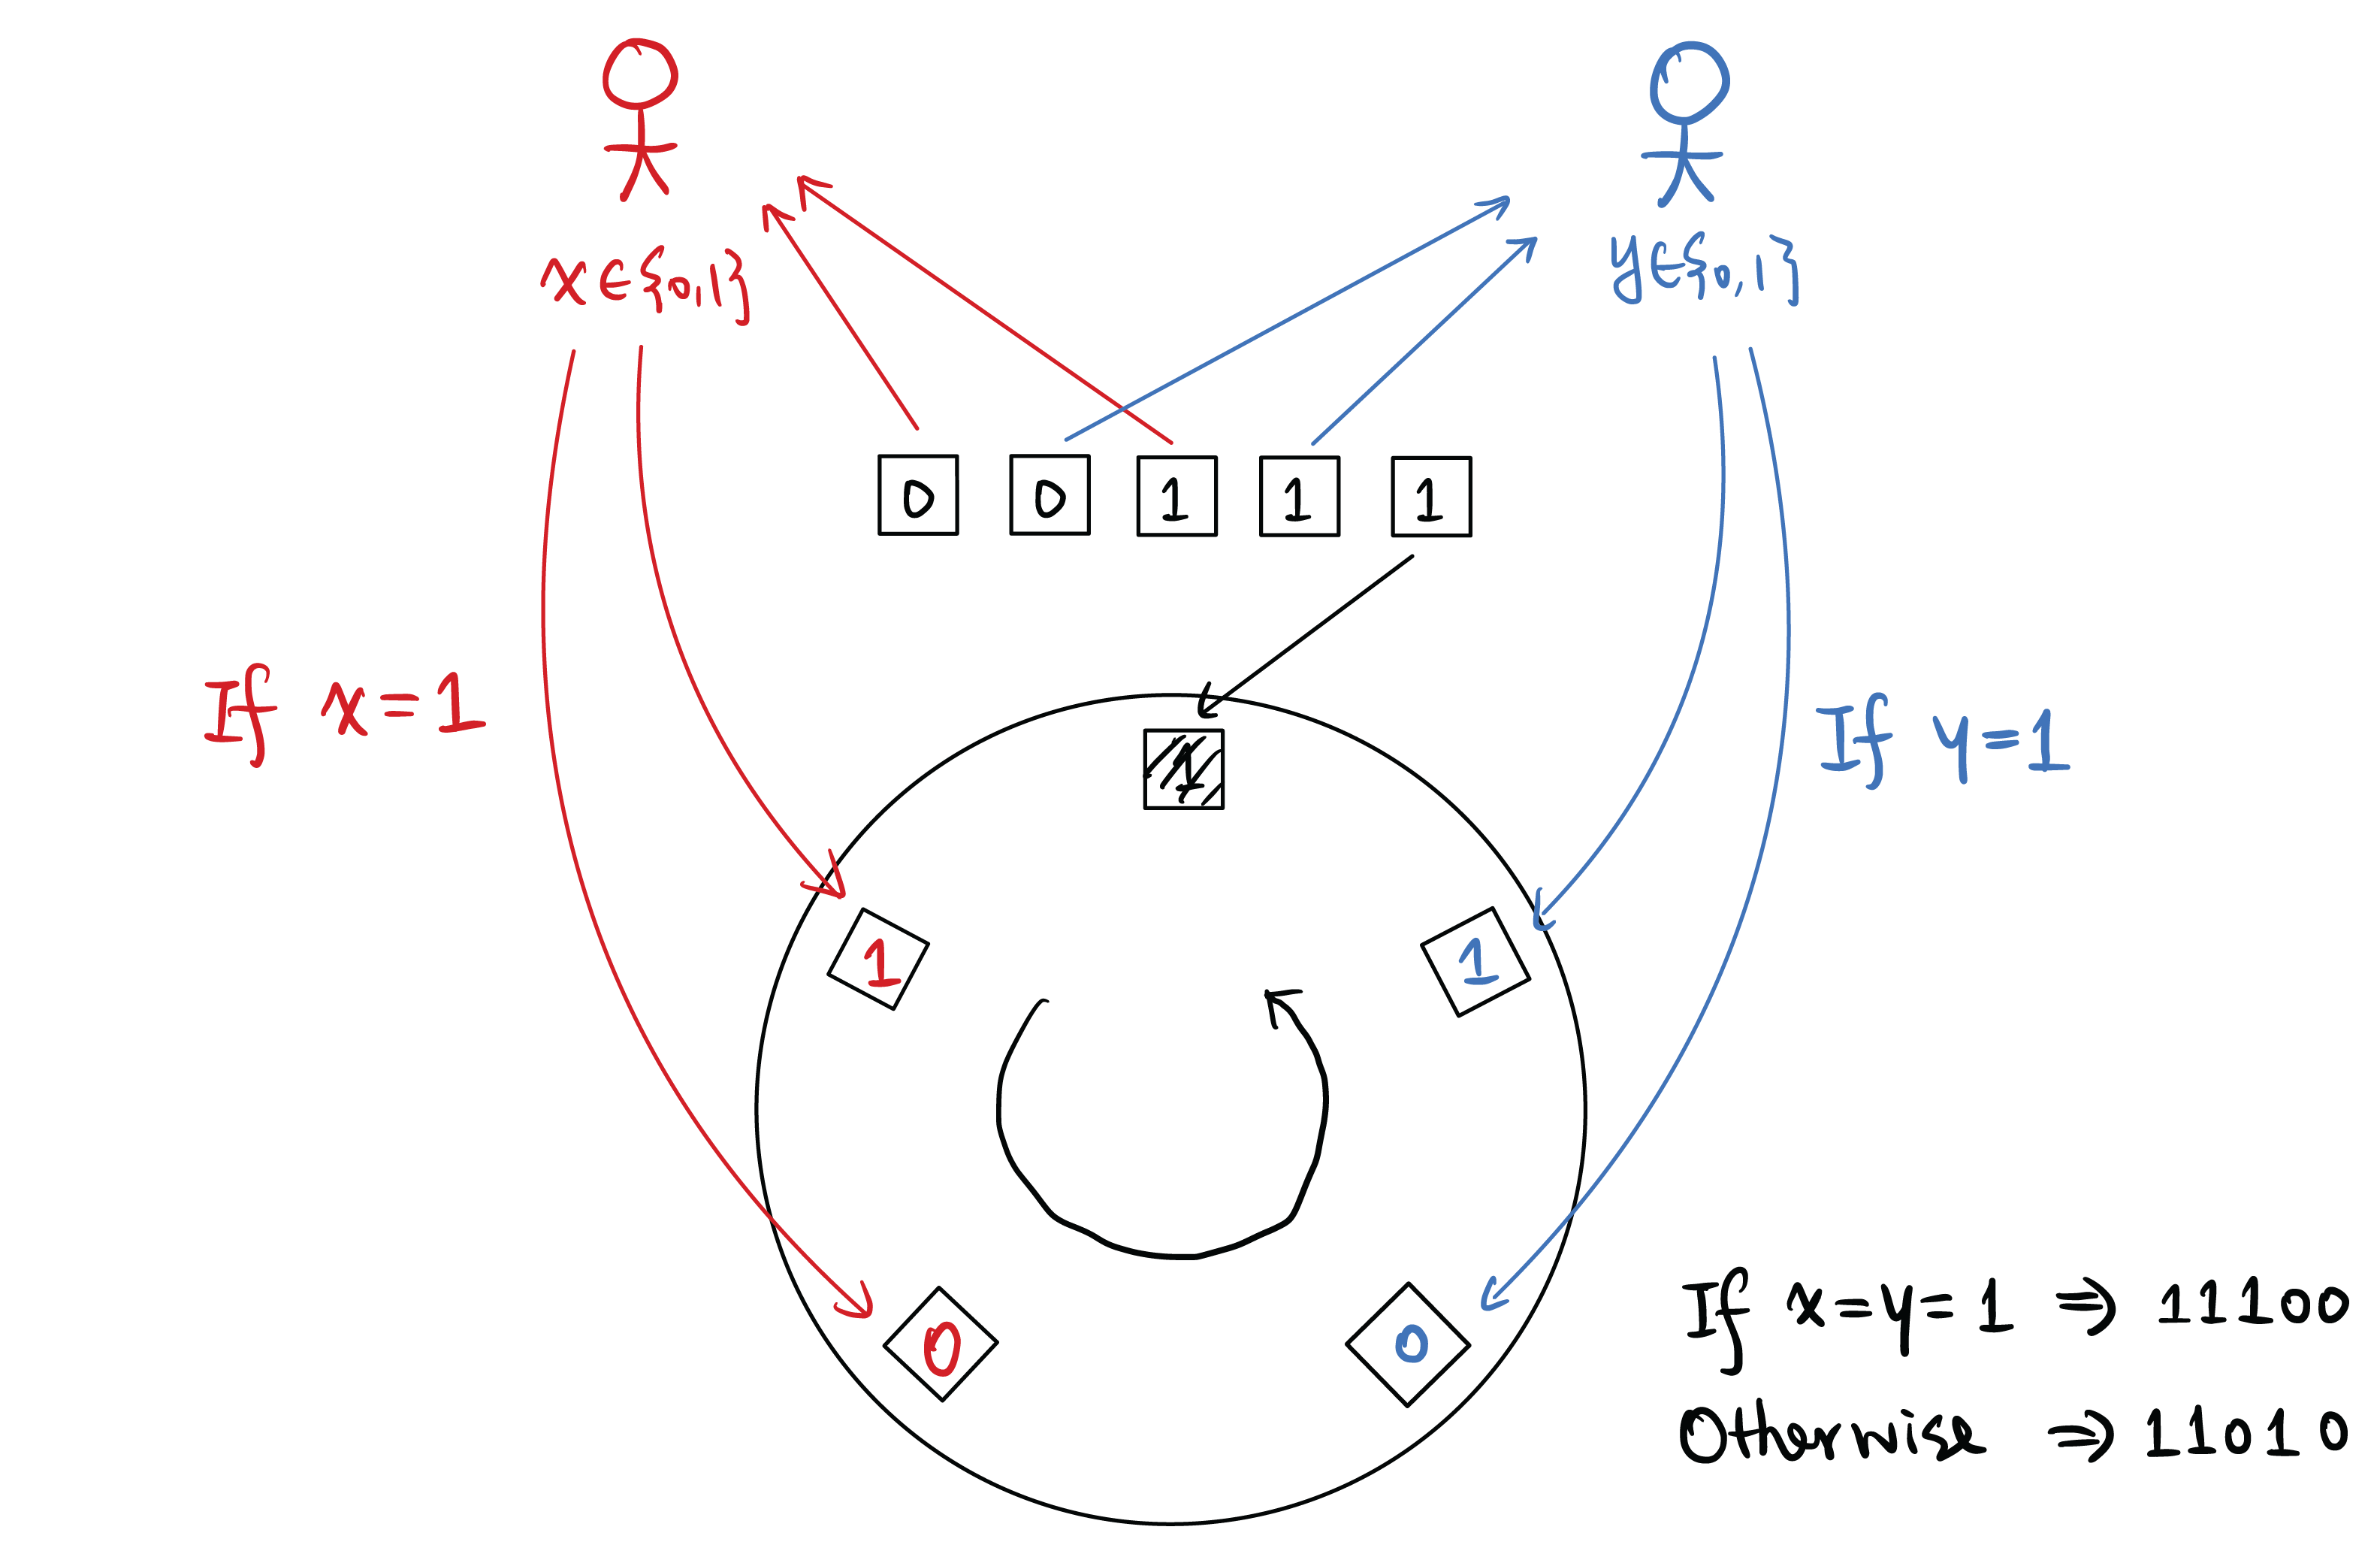
\includegraphics[width=0.9\textwidth]{images/2023-01-26/private_dating.png}
    \end{center}

    Alice and Bob each have identical $0, 1$ cards (each of the $0$ and $1$ cards are indistinguishable from cards of the same value). Alice places her cards on the 2 slots in some order, and Bob does the same.

    They then spin the table around and reveal all the cards, learning $x\land y$.

    If $x = 1$, Alice places it as $1$ on top of $0$, and if $y = 1$, Bob places it as $1$ on top of $0$ as well. Otherwise, they flip them. If $x = y = 1$, then the $0$'s will be adjacent. If $x \neq y$, the order will be $1,1,0,1,0$ (the $0$'s are not adjacent), regardless of which of Alice or Bob produced $x = 0$ (or both!).
\end{example*}

\emph{This is a toy example! It doesn't use cryptography at all! Two parties have to sit in front of a table. This is called card-based cryptography. We will be using more secure primitives.}

\subsection{Fully Homomorphic Encryption}
We'll come back to the secure messaging example.

Alice wants to send Bob a message. She encrypts it somehow and sends a ciphertext $c_1 = \mathsf{Enc}(m_1)$. A nice feature for some encryption schemes is for Eve to do some computation homomorphically on the ciphertexts. Eve might possibly want to add ciphertexts (that leads to plaintext adding)
\[c_1 = \mathsf{Enc}(m_1),\ c_2 = \mathsf{Enc}(m_2)\Rightarrow c' = \mathsf{Enc}(m_1 + m_2)\]
or perhaps $c'' = \mathsf{Enc}(m_1\cdot m_2)$, or compute arbitrary functions. \emph{Sometimes}, this is simply adding $c_1 + c_2$, but usually not.

\begin{center}
    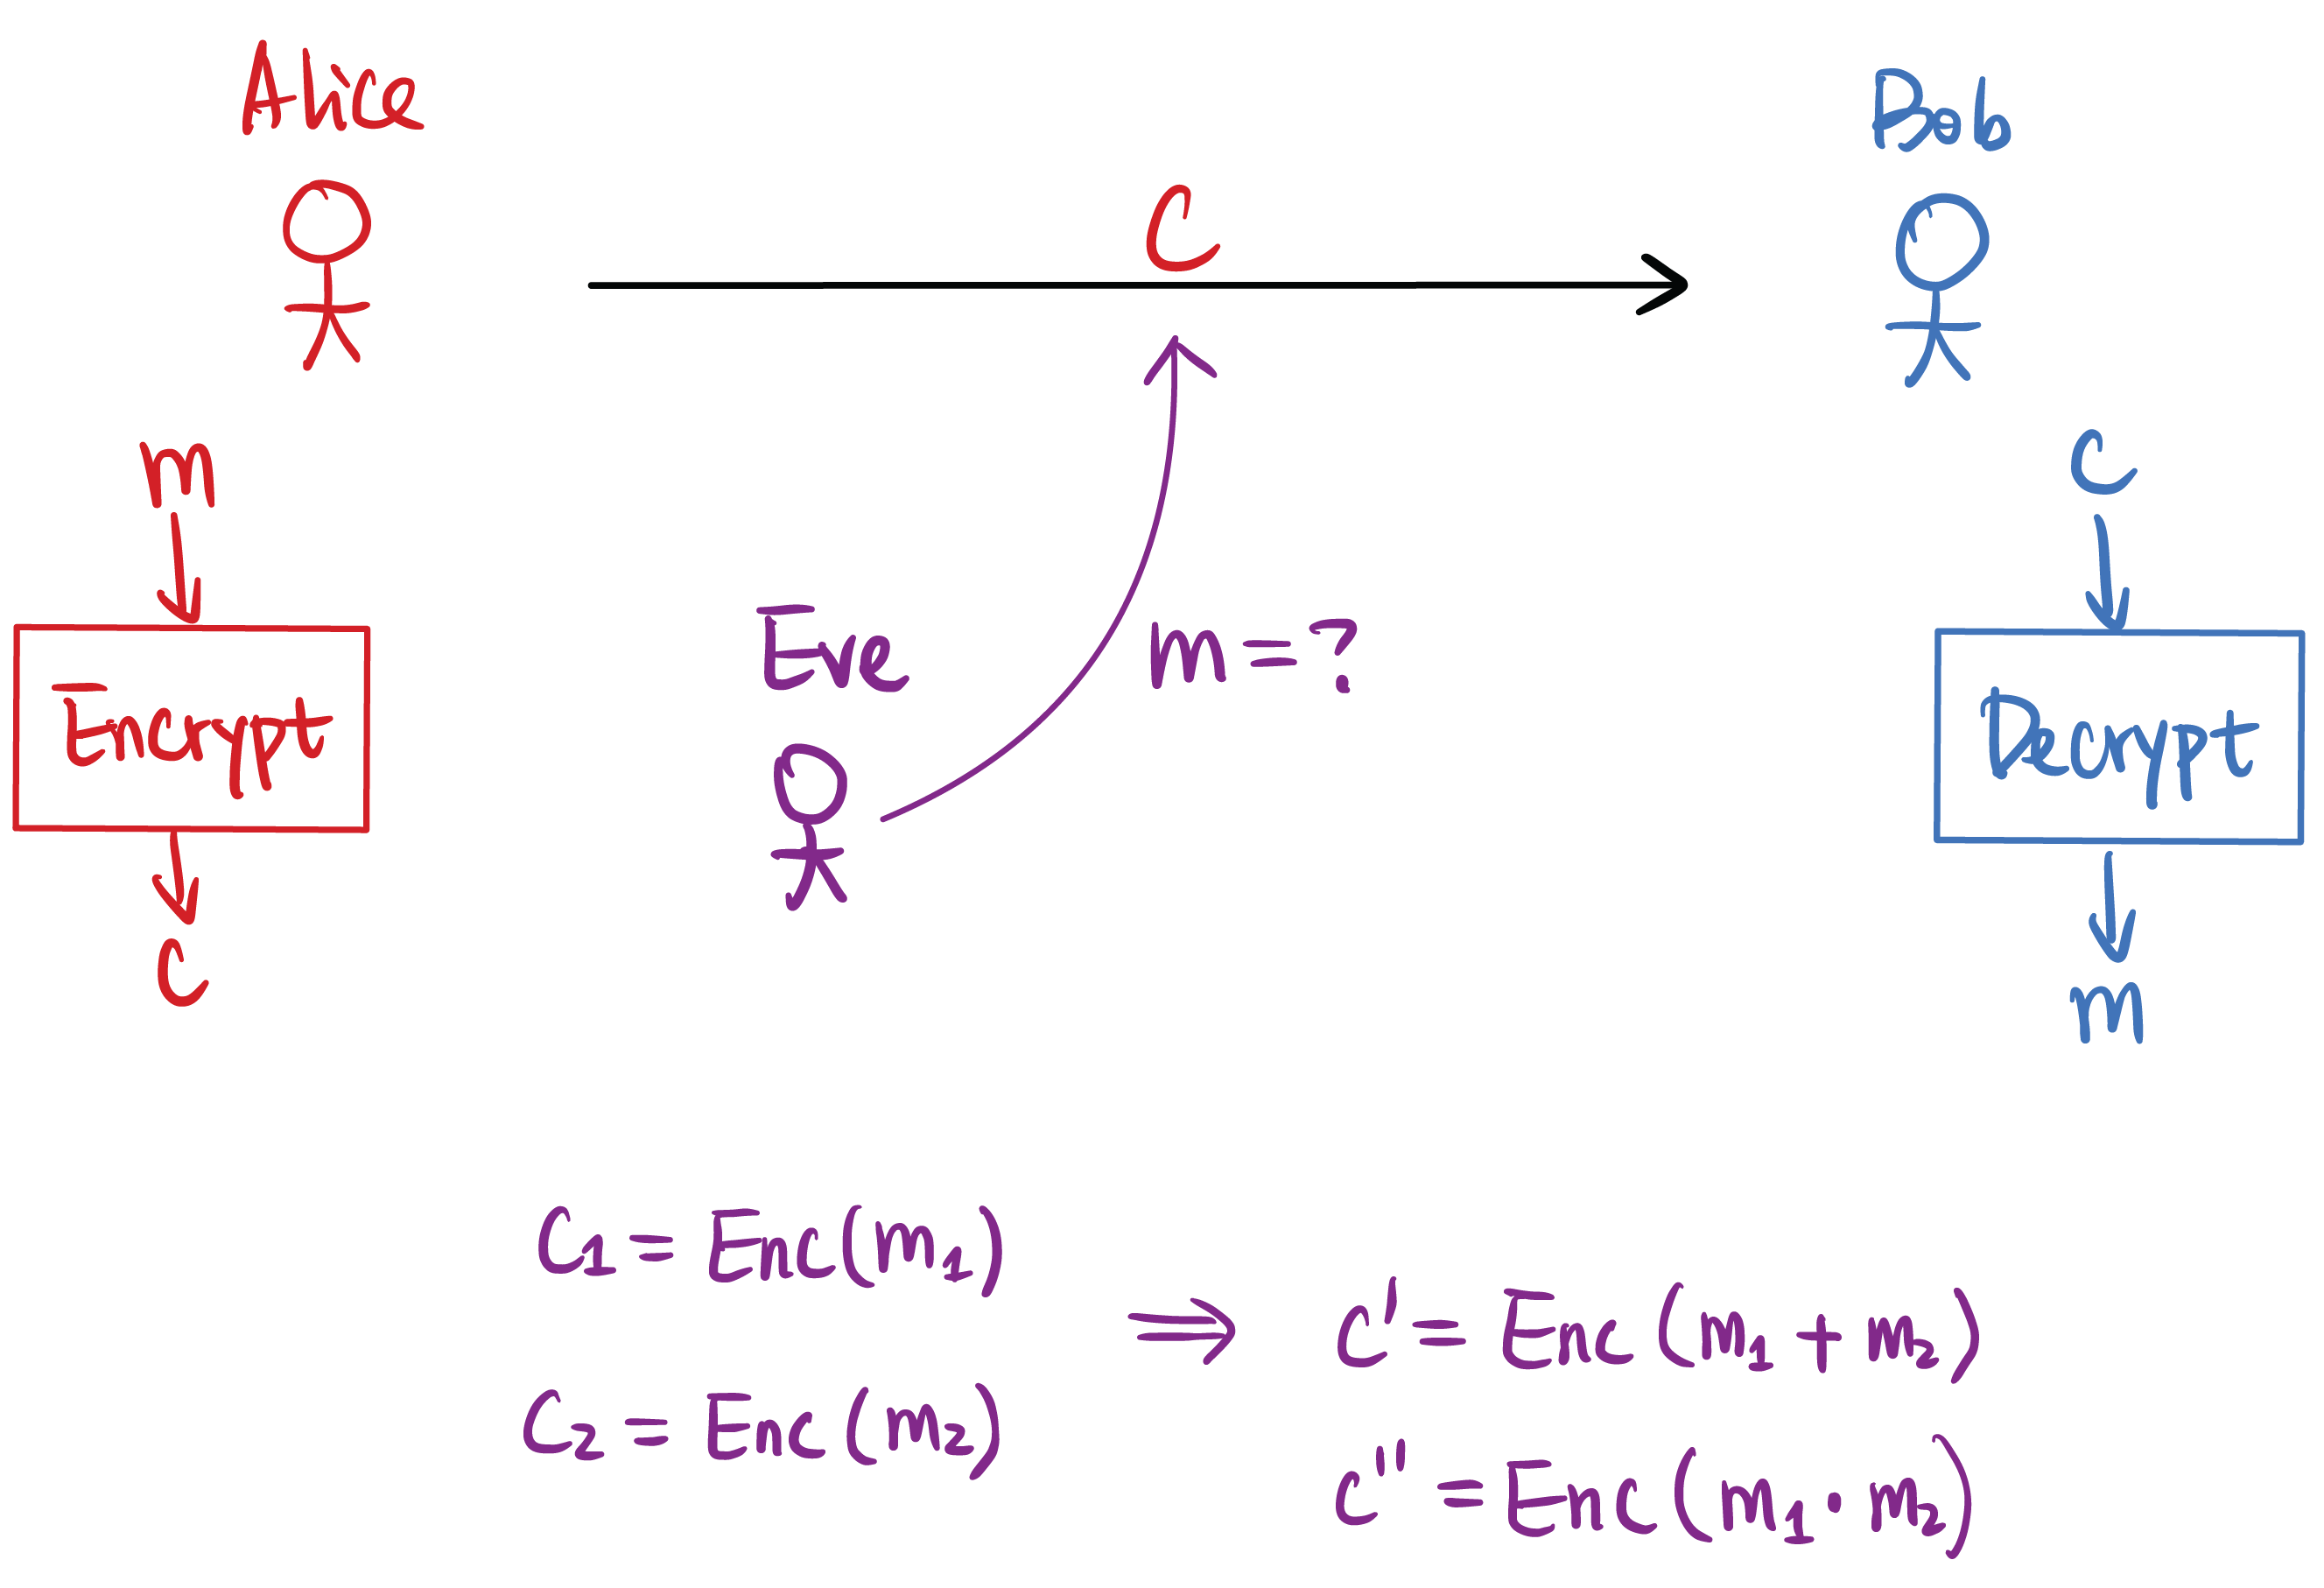
\includegraphics[width=0.9\textwidth]{images/2023-01-26/homomorphic_encryption.png}
\end{center}

We want to hopefully compute any function in polynomial time!

\begin{example*}[Outsourced Computation]
    Alice has some messages but doesn't have enough compute. There is a server that has \emph{a lot} of compute!

    \begin{center}
        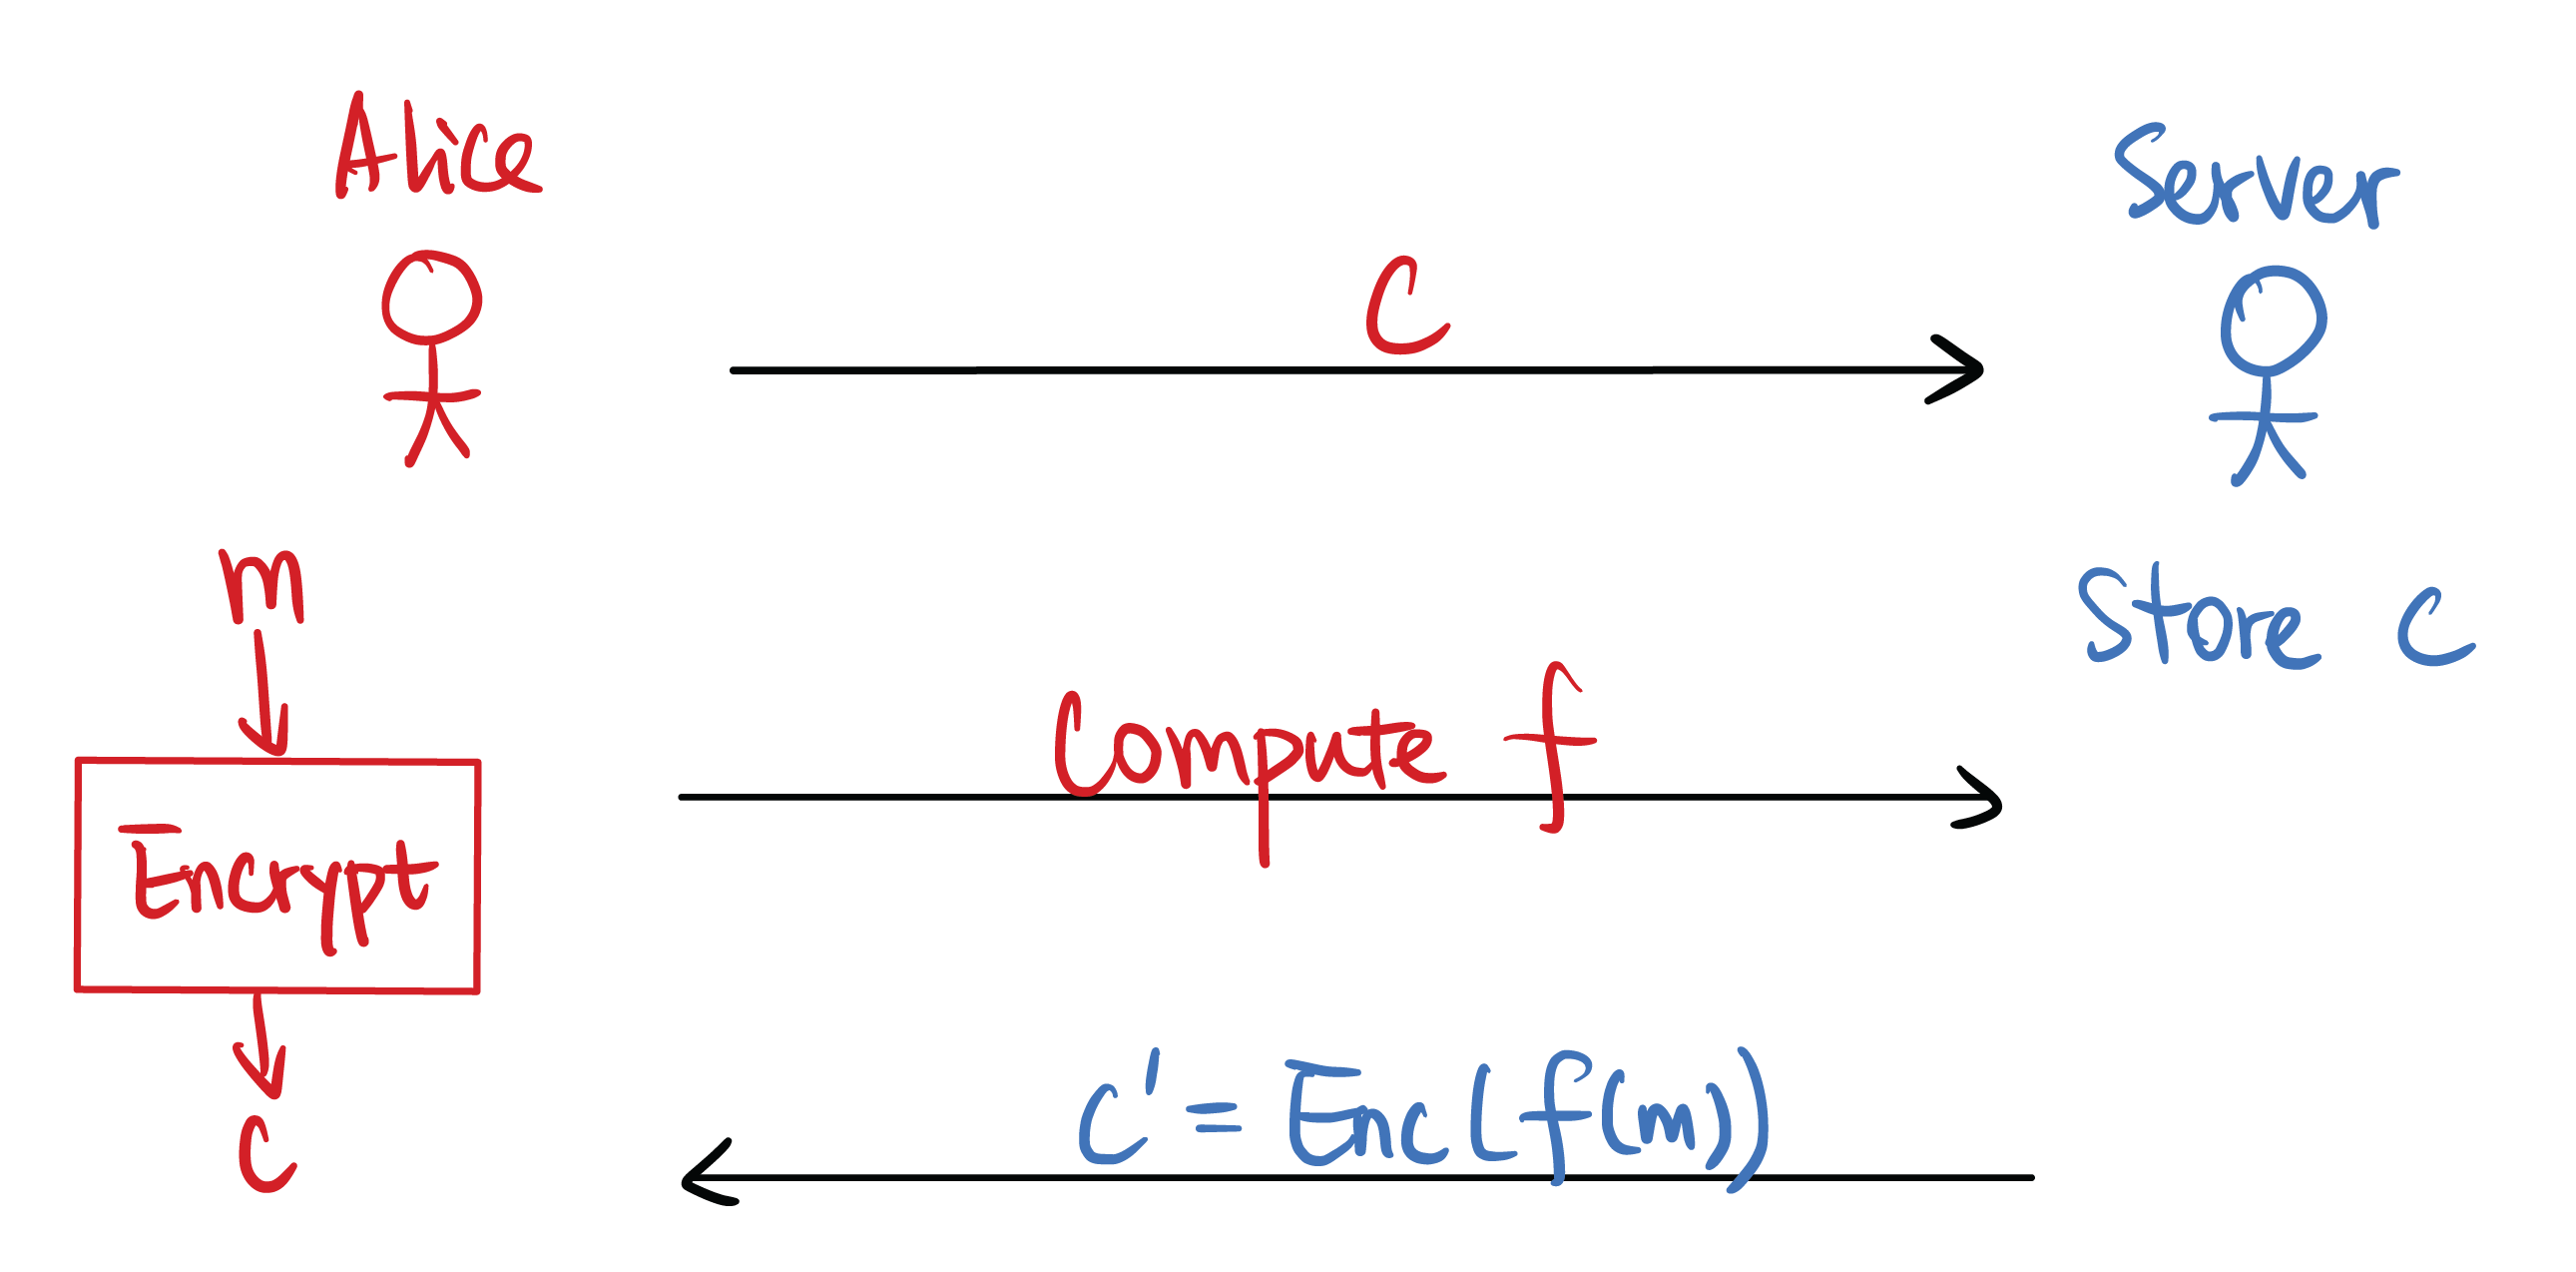
\includegraphics[width=0.9\textwidth]{images/2023-01-26/outsourced_computation.png}
    \end{center}

    Alice encrypts her data and stores it in the server. At some point, Alice might want to compute a function on the encrypted data on the server, without the server revealing the original data.

    This is an example of how fully homomorphic encryption can be useful.
\end{example*}

\begin{remark*}
    This problem was not solved until 2009 (when Peihan started her undergrad). Theoretically, it doesn't even seem that possible! Being able to compute functions on ciphertexts that correspond to functions on plaintexts.
\end{remark*}

To construct fully-homomorphic encryption, we'll be using lattice-based cryptography which is a post-quantum secure!

\subsection{Further Topics}
We might cover some other topics:
\begin{itemize}
    \item Differential Privacy
    \item Crypto applications in machine learning
    \item Crypto techniques used in the blockchain\footnote{One important techniques is Zero-Knowledge proofs, for example.}
\end{itemize}
\emph{What else would you like to learn? What else do you want to understand?} Do go through the semester with these in mind! \emph{How do I log into Google? How do I send messages to friends?}

Feel free to let us know on Ed!

\subsection{Q \& A}

\begin{itemize}
    \item \emph{What is the difference between CSCI 1515 and CSCI 1510 or MATH 1580?}
    
    CSCI 1510 is essentially ``theoretical cryptography.'' It covers formal definitions and constructions and proofs. There is no coding, just proofs.

    MATH 1580 considers crypto from the mathematical perspective. They try to understand some of the computational assumptions we assume from a mathematical standpoint. I.e. why is factoring hard to compute, and what is the best algorithm to compute it? In CS, we simply assume factoring is hard. MATH 1580 is more similar to number theory and group theory.

    \item \emph{If you've taken MATH 1580 and CSCI 1515, would you still recommend taking CSCI 1510?}
    
    There are still more things to learn from CSCI 1510. There is still more theory and it is a much more challenging course from the theoretical perspective. There are more rigorous proofs and reductions in CSCI 1510 that we do not cover in CSCI 1515.

    \item \emph{Why C++}

    Existing crypto libraries are mostly in C++ and most students have seen C/C++ in either cs33 or cs300. We did, however, consider implementing everything in Rust!
\end{itemize}

%!TEX root = ../notes.tex
\section{January 29, 2024}
\label{20240129}
\subsection{Logistics}
There's an EdStem post asking about topics you're interested, feel free to keep on posting!

We acknowledge the synchronization issues with Panopto. For now, if you want to watch the lecture recordings, you can use the Zoom link linked from the course home page. We can manually sync up EdStem but Panopto cannot be synced up, unfortunately.

\subsection{Encryption Schemes}
This lecture we'll cover encryption schemes. We briefly mentioned what encryption schemes were last class, we'll dive into the technical content: how we construct them, assumptions, RSA, ElGamal, etc.

Fundamentally, an encryption scheme protects message secrecy. If Alice wants to communicate to Bob, Alice will encrypt a message (plaintext) using some key which gives her a ciphertext. Sending the ciphertext through Bob using a public channel, Bob can use the key to decrypt the ciphertext and recover the message. An eavesdropper in the middle will have no idea what message has been transmitted.

\begin{center}
    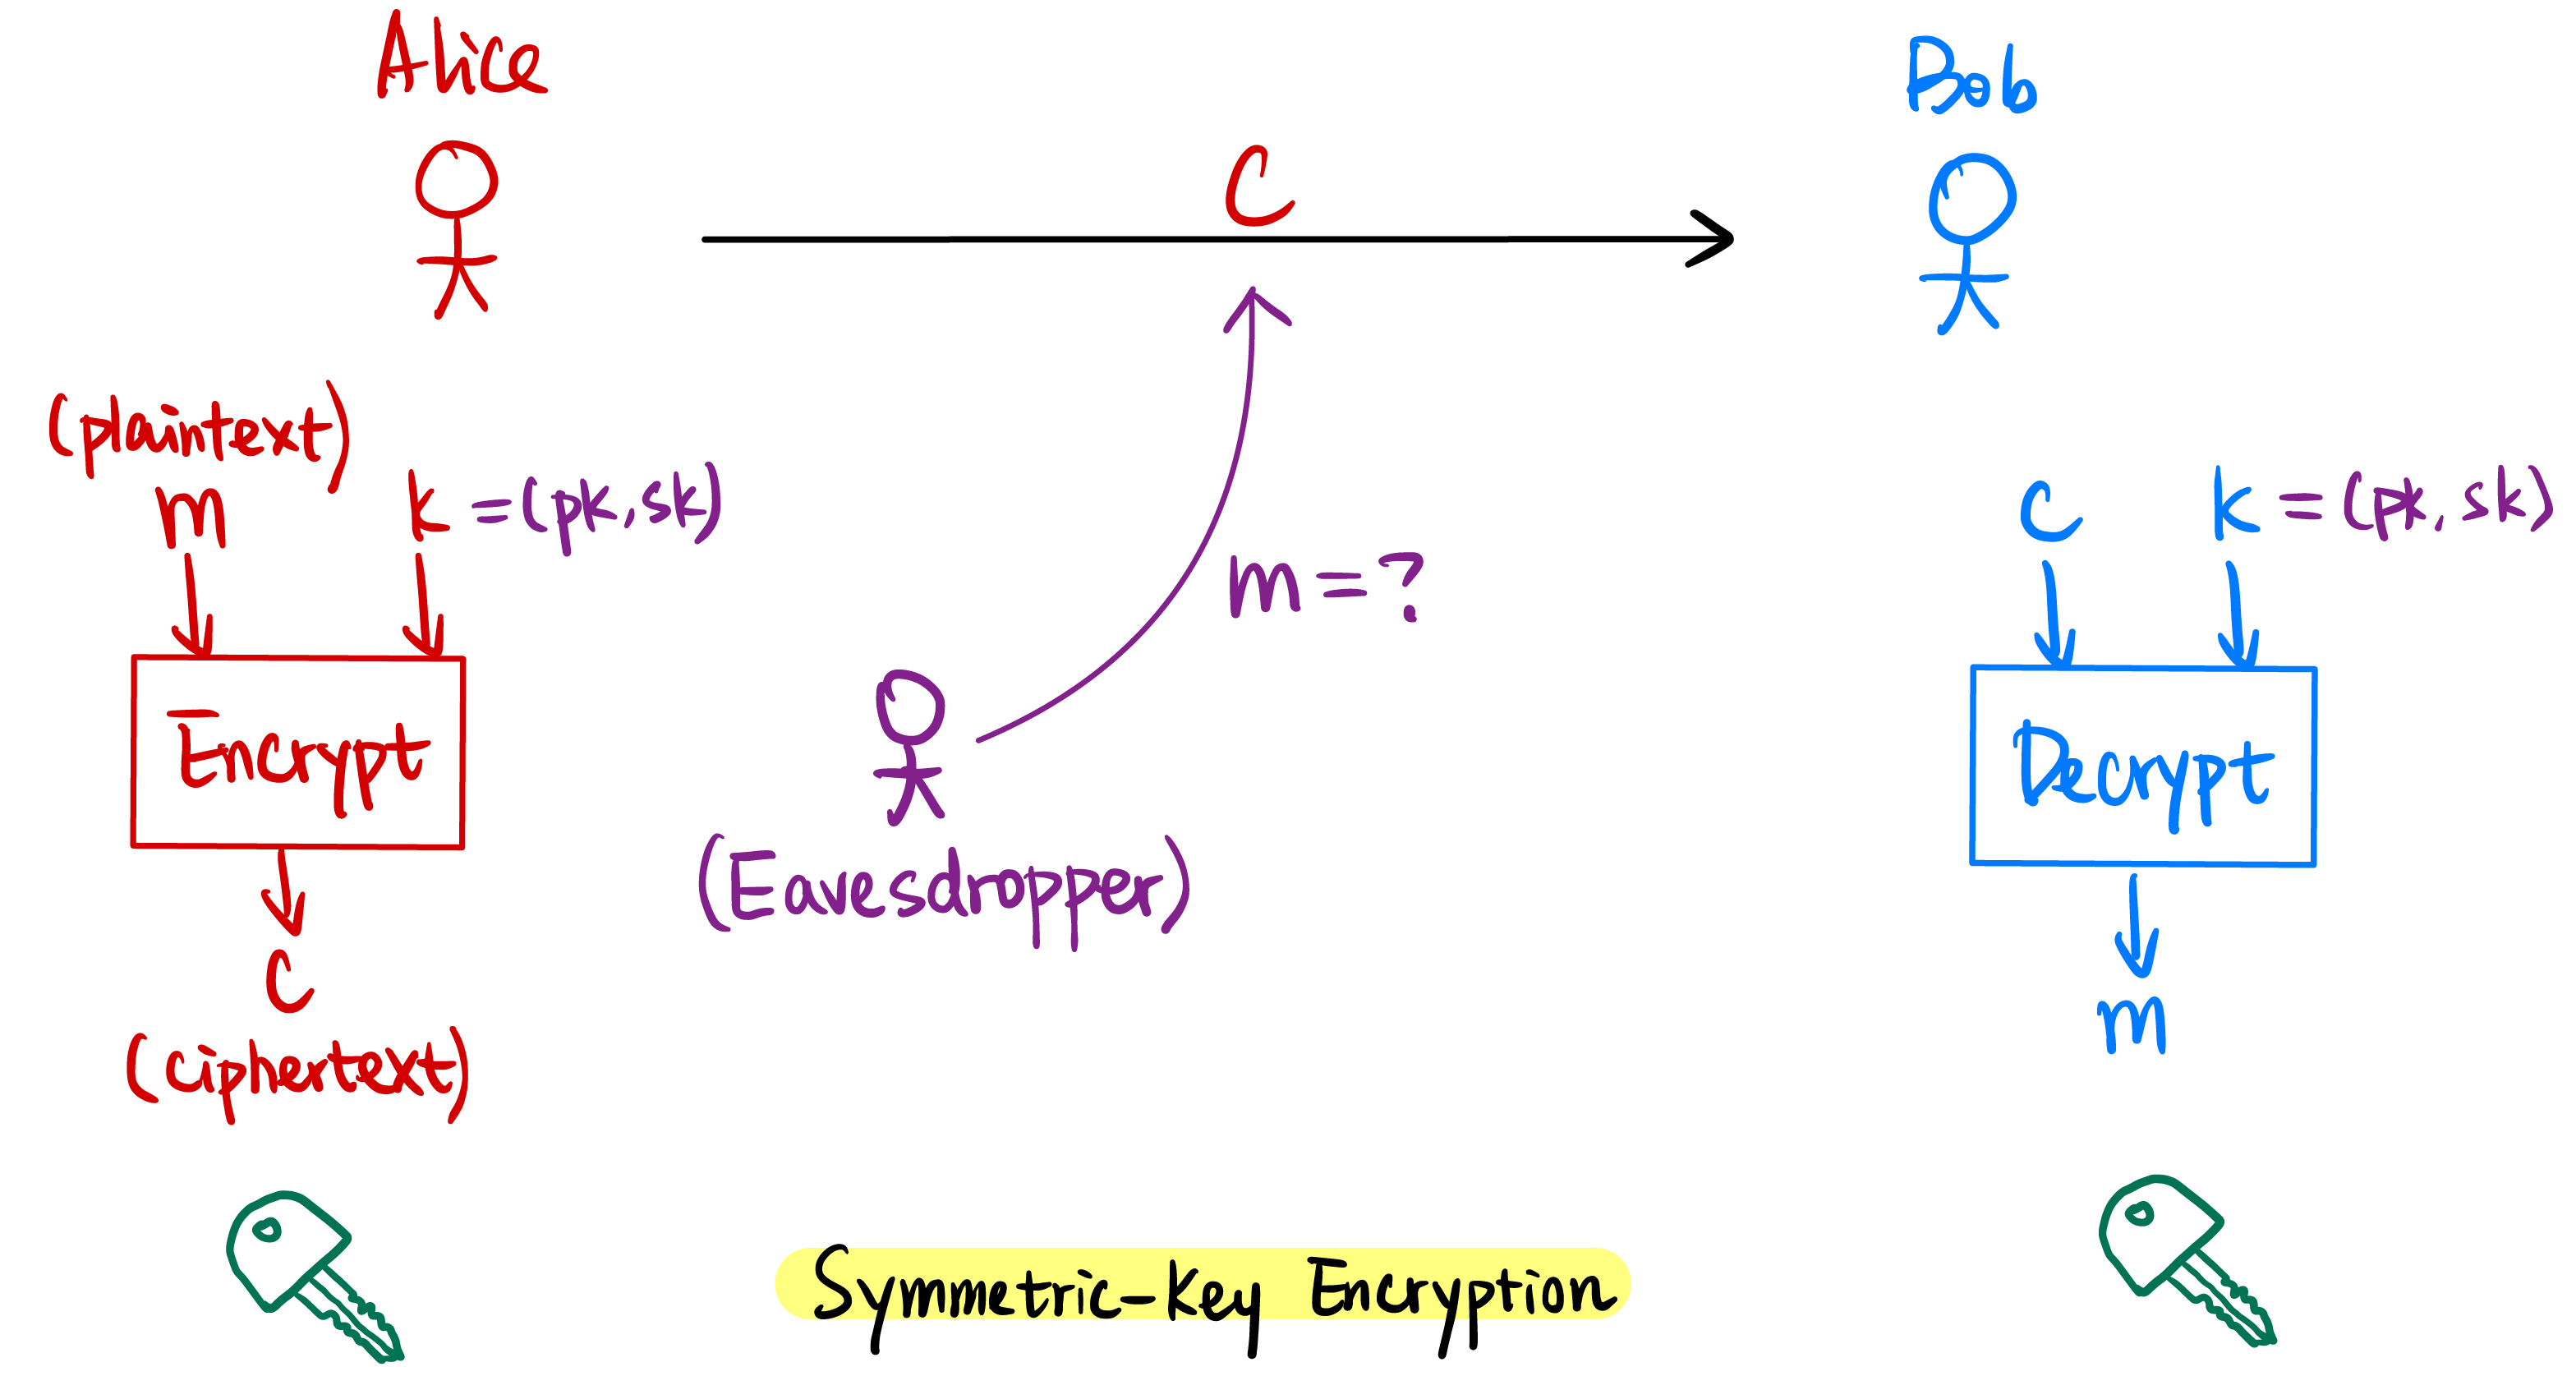
\includegraphics[width=0.8\textwidth]{images/2023-01-31/ske-intro.png}
\end{center}

In this case, they are using a shared key, which we called secret-key encryption or symmetric-key encryption.

A stronger version of private-key encryption is called public-key encryption. Alice and Bob do not need to agree on a shared secret key beforehand. There is a keypair $(pk, sk)$, a \emph{public} and \emph{private} key.

\begin{center}
    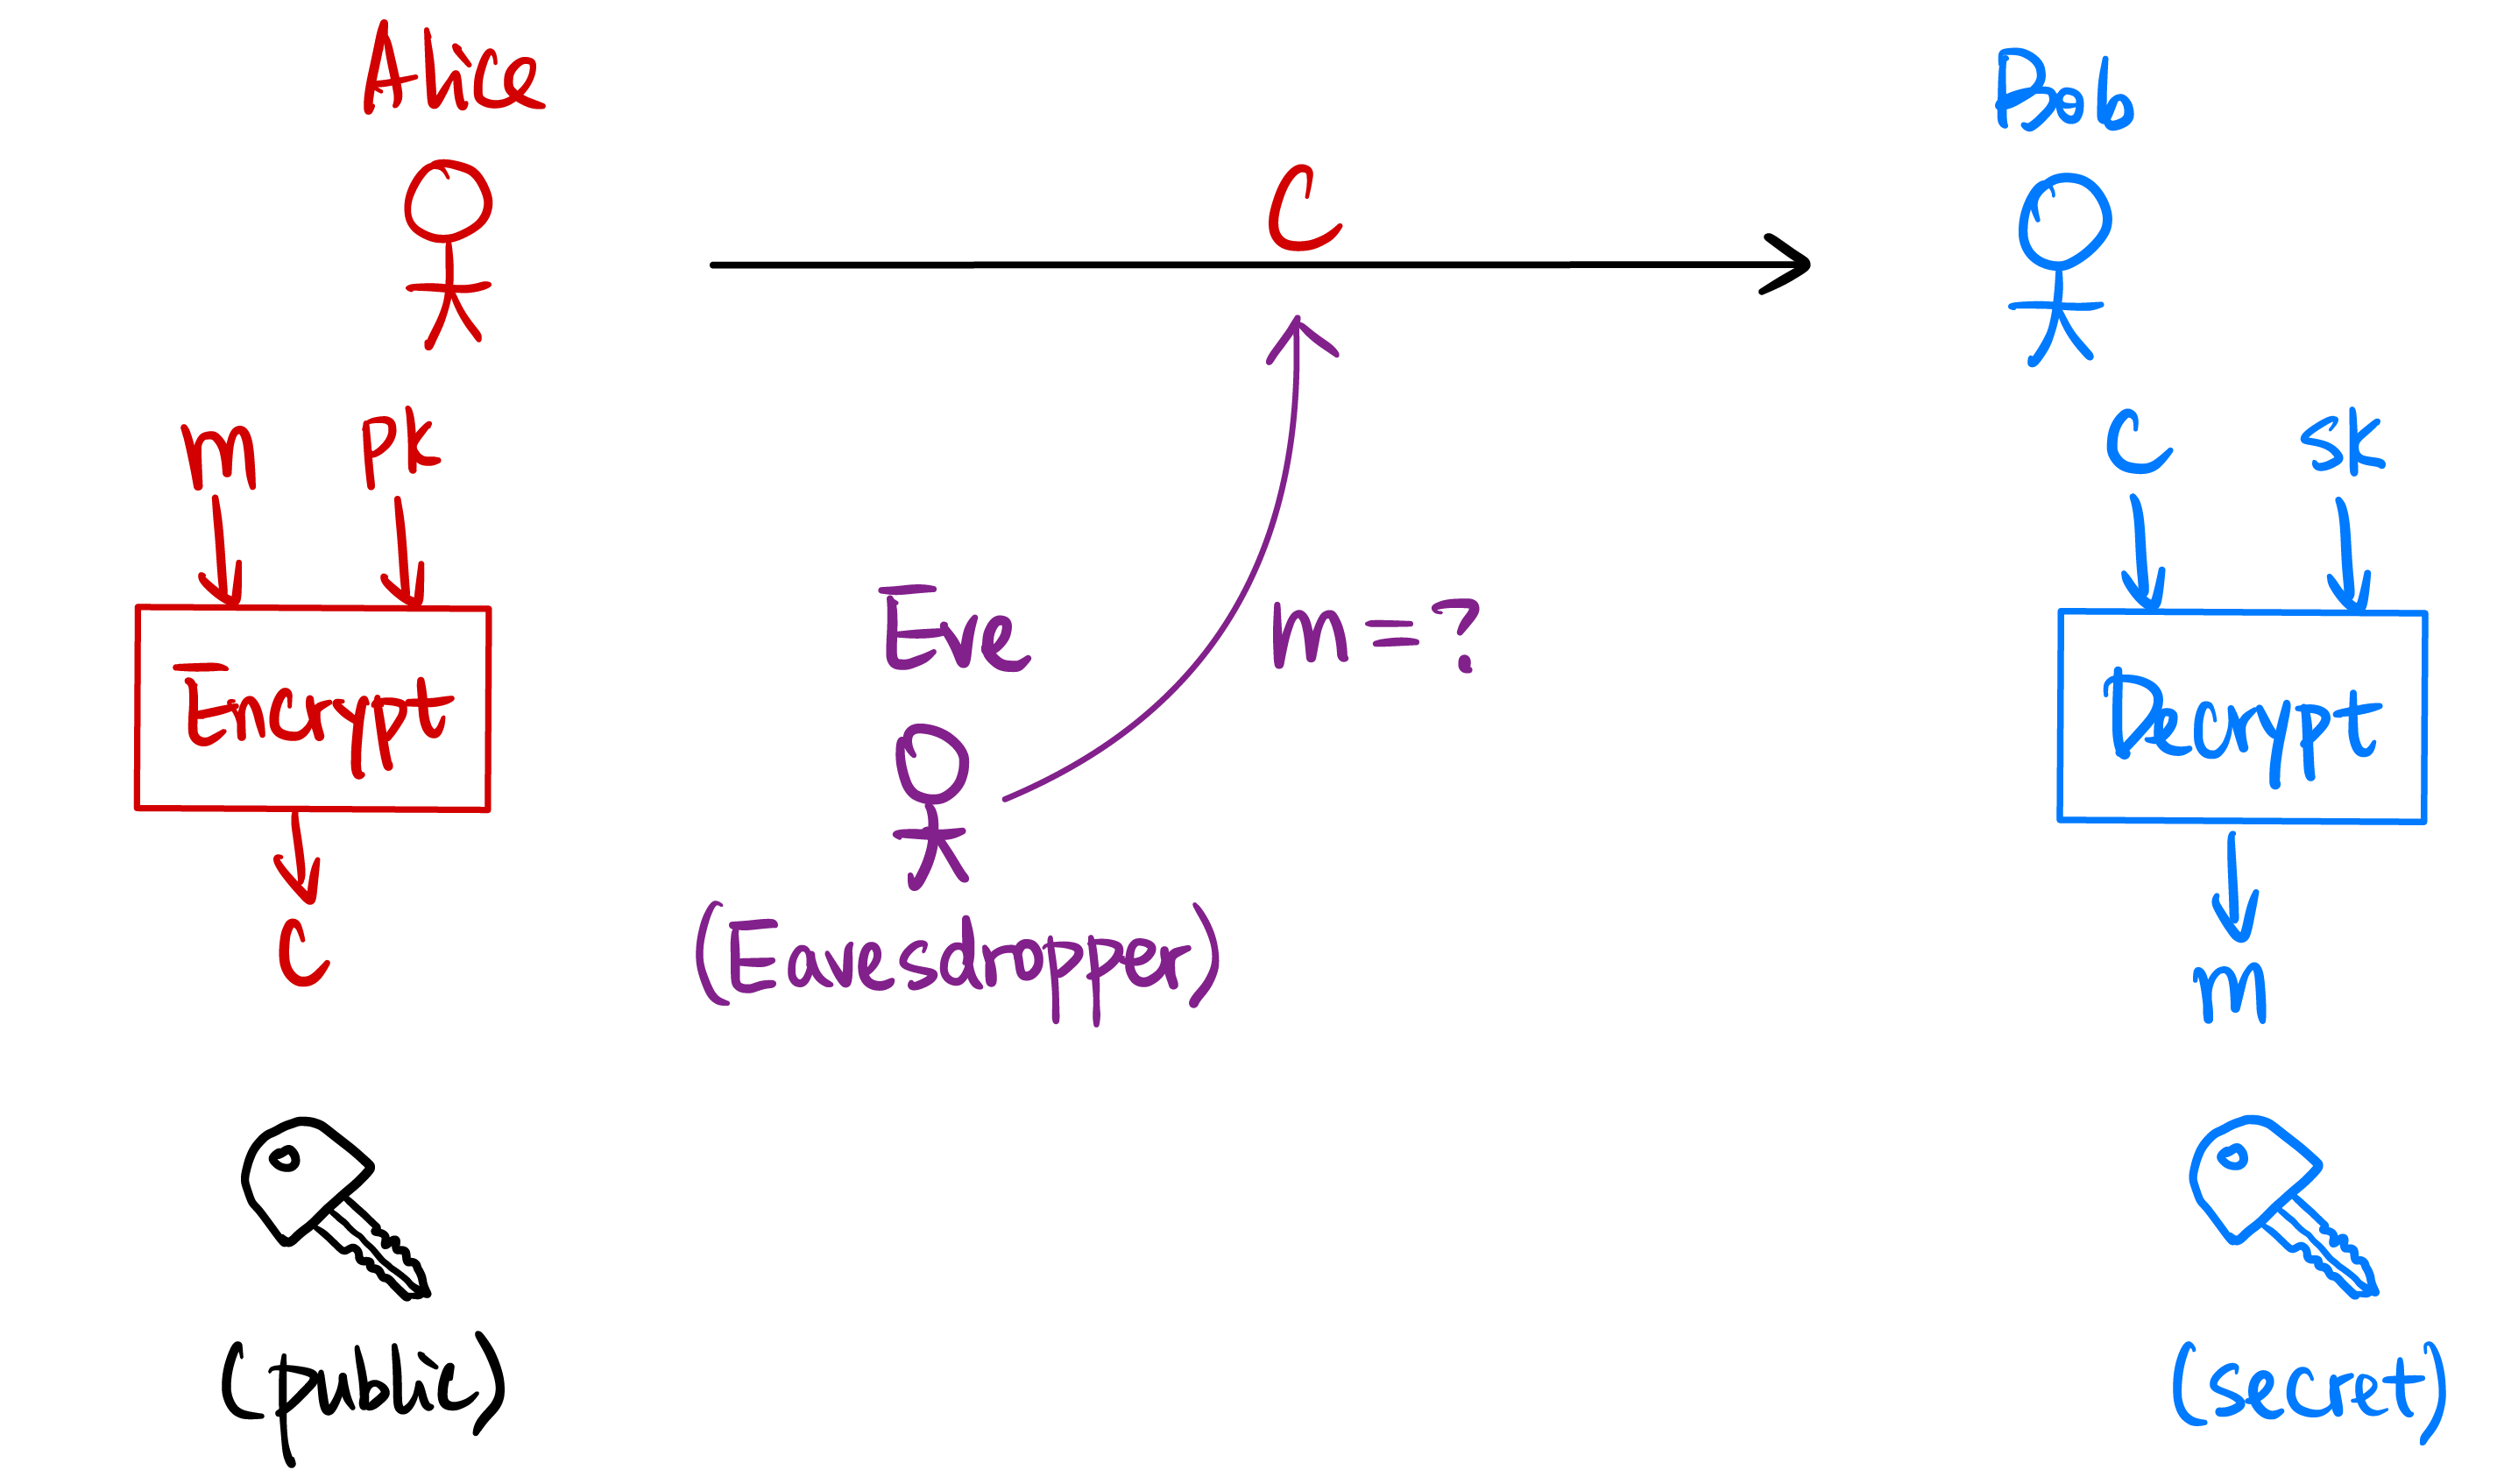
\includegraphics[width=0.8\textwidth]{images/2023-01-31/pke-intro.png}
\end{center}

\subsubsection{Syntax}
\begin{definition}[Symmetric-Key Encryption]
    A symmetric-key encryption (SKE) scheme contains 3 algorithms, $\Pi = (\mathsf{Gen}, \mathsf{Enc}, \mathsf{Dec})$.

    \begin{description}
        \item[Generation.] Generates key $k\leftarrow \mathsf{Gen}$.
        \item[Encryption.] Encrypts message $m$ with key $k$, $c\leftarrow \mathsf{Enc}(k, m)$, which we sometimes write as $\Enc_k(m)$.
        \item[Decryption.] Decrypts using key $k$ to retrieve message $m$, $m := \Dec(k, c)$, or written as $\Dec_k(c)$.
    \end{description}
    Note the notation $\leftarrow$ and $:=$ is different. In the case of generation and encryption, the produced key $k$ or $c$ follows a \emph{distribution} (is randomly sampled), but we had better want decryption to be deterministic in producing the message.
\end{definition}

\begin{definition}[Public-Key Encryption]
    A public-key encryption (PKE) scheme $\Pi = (\Gen, \Enc, \Dec)$ contains the same $3$ algorithms,

    \begin{description}
        \item[Generation.] Generate keys $(pk, sk)\leftarrow \Gen$.
        \item[Encryption.] Use the public key to encrypt, $c\leftarrow \mathsf{Enc}(pk, m)$ or $\Enc_{pk}(m)$.
        \item[Decryption.] Use the secret key to decrypt, $m:=\Dec(pk, c)$ or $\Dec_{sk}(c)$.
    \end{description}

\end{definition}

\begin{ques*}
    If we can construct public-key encryption, why do we even bother with secret-key encryption? We could just use the $(pk, sk)$ pair for our secret key, and this does the same thing.
\end{ques*}

\begin{enumerate}
    \item First of all, public-key encryption is almost always \emph{more expensive}. Symmetric-key encryption schemes give us efficiency.
    \item Public-key encryption relies on much stronger computational assumptions.
\end{enumerate}

\subsubsection{Symmetric-Key Encryption Schemes}
\begin{definition}[One-Time Pad]
    Secret key is a uniformly randomly sampled $n$ bit string $k\sampledfrom \{0, 1\}^n$.

    \begin{center}
        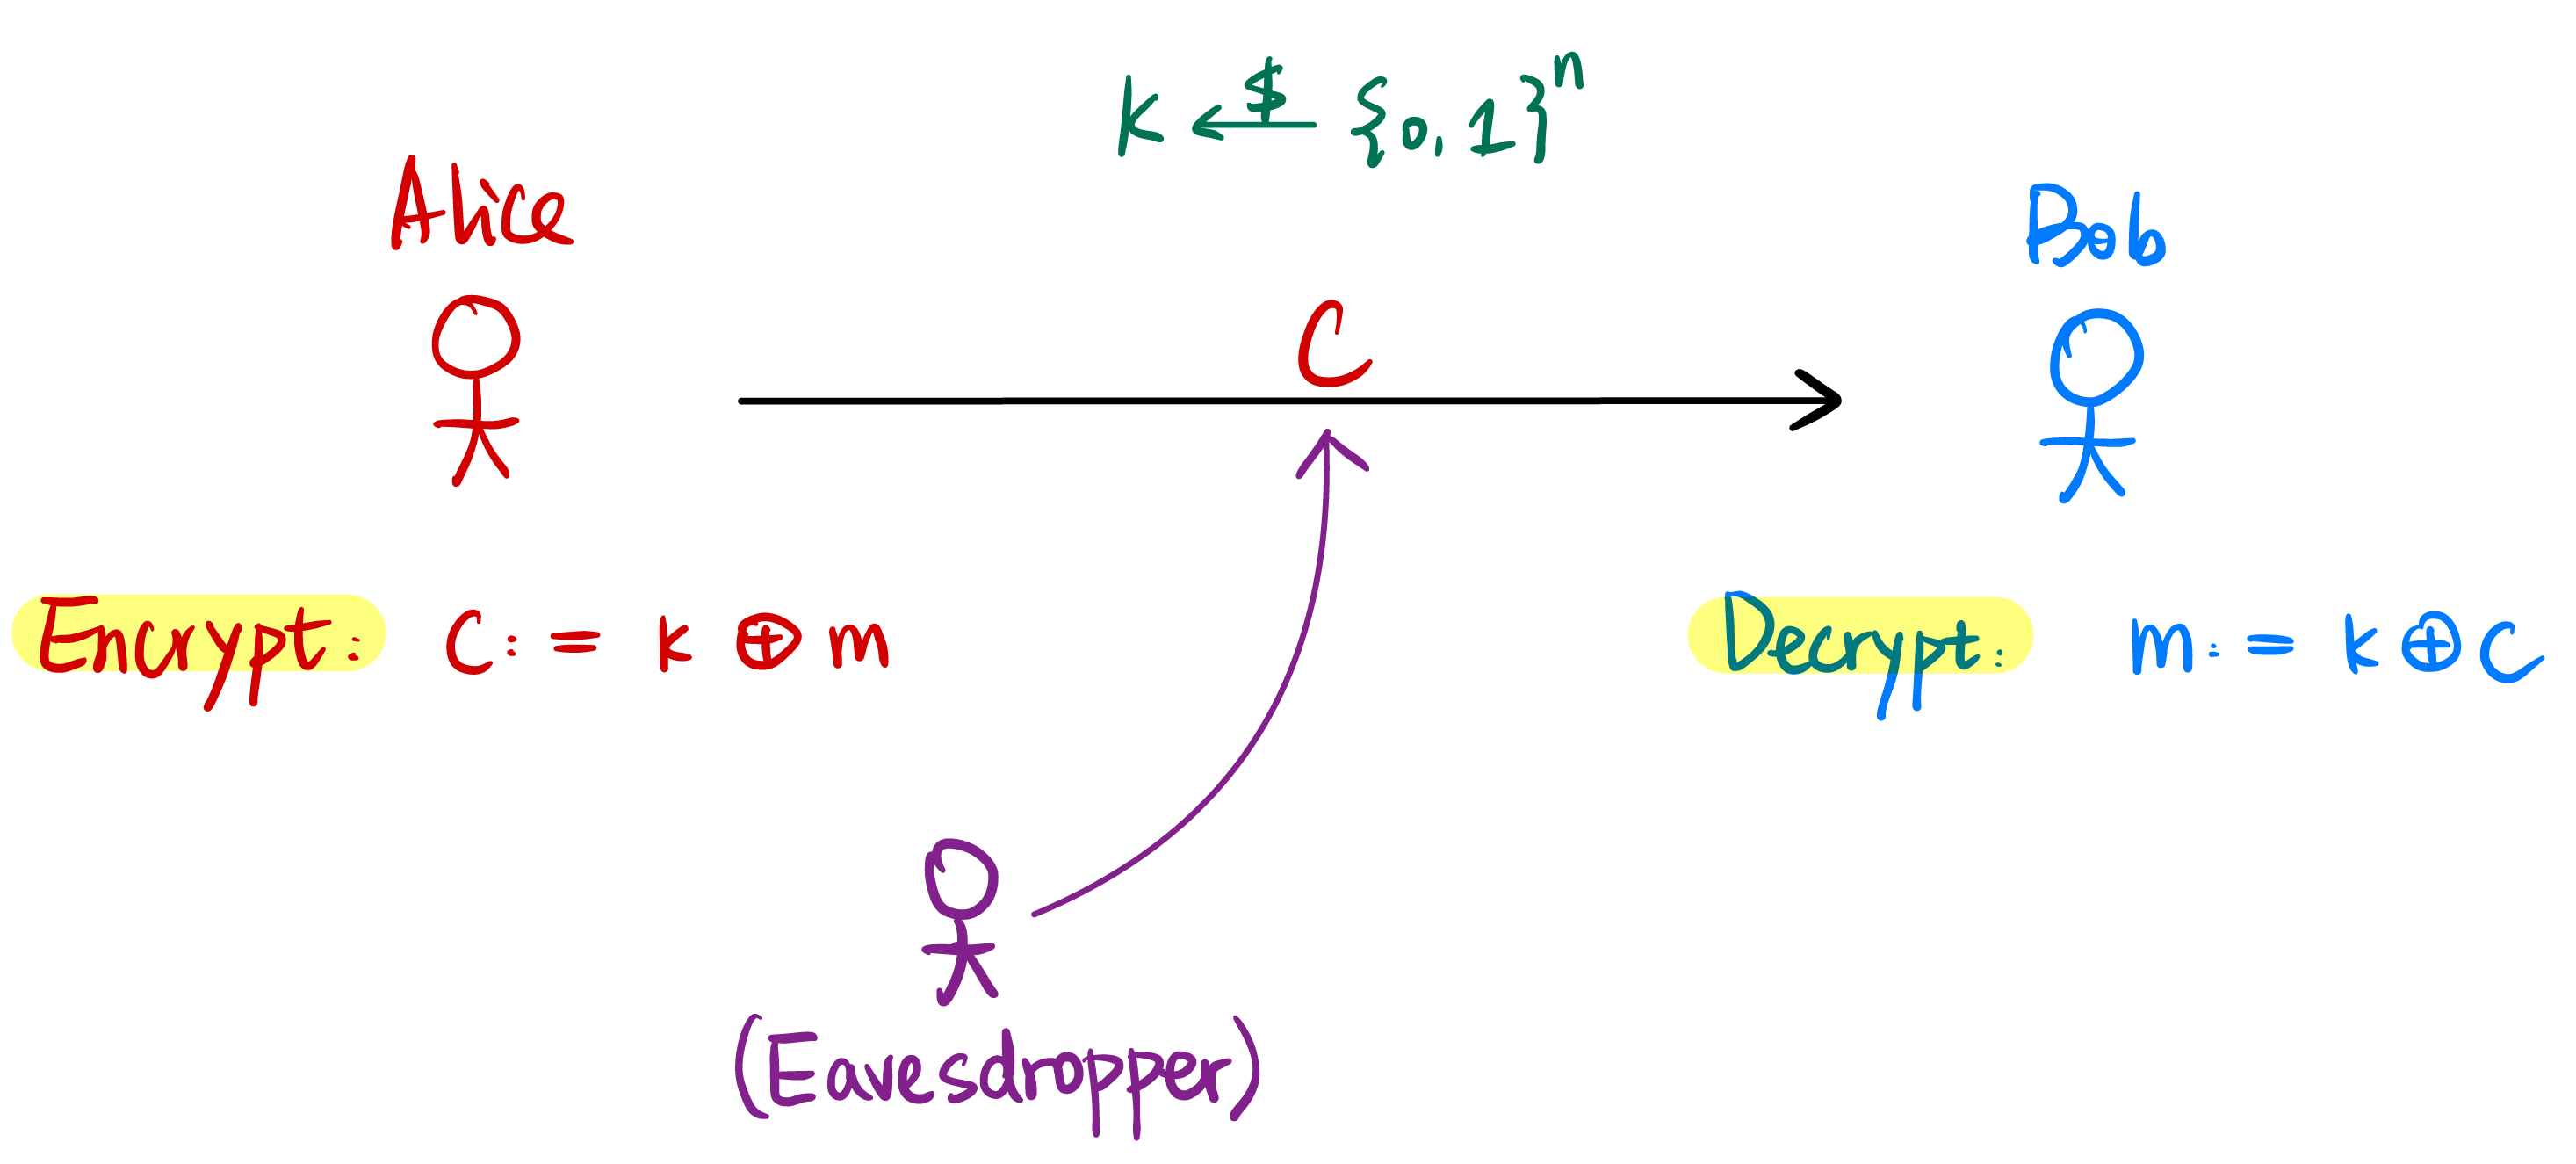
\includegraphics[width=0.7\textwidth]{images/2023-01-31/otp-defn.png}
    \end{center}

    \begin{description}
        \item[Encryption.] Alice uses the secret key and bitwise-$\mathsf{XOR}$ with the plaintext.
            \begin{align*}
                \begin{split}
                    \text{secret key}\quad k       & = 0100101 \\
                    \oplus\text{ plaintext}\quad m & = 1001001 \\ \eqline
                    \text{ciphertext}\quad c       & = 1101100
                \end{split}
            \end{align*}
        \item[Decryption.] Bob uses the secret key and again bitwise-$\mathsf{XOR}$ with the ciphertext
            \begin{align*}
                \begin{split}
                    \text{secret key}\quad k        & = 0100101 \\
                    \oplus\text{ ciphertext}\quad c & = 1101100 \\ \eqline
                    \text{plaintext}\quad c         & = 1001001
                \end{split}
            \end{align*}
    \end{description}

    This is widely used in cryptography, called \emph{masking} or \emph{unmasking}.
\end{definition}

\begin{ques*}
    Why is this correct?
\end{ques*}
An $\mathsf{XOR}$ done twice with the same choice bit $b$ is the identity. Or, an element is its own inverse with the $\mathsf{XOR}$ operator.

\begin{ques*}
    Why is this secure?
\end{ques*}

We can think about this as the distribution of $c$. $\forall m\in \{0, 1\}^n$, the encryption of $m$ is uniform over $\{0, 1\}^n$ (since $k$ was uniform).

Another way to think about this is that for any two messages $m_0, m_1\in\{0, 1\}^n$, $\Enc_k(m_0)\equiv \Enc_k(m_1)$. That is, the encryptions follow the \emph{exact same} distribution. In this case, they are both uniform, but this is not always the case.

\begin{ques*}
    Can we reuse $k$? Should we use the same key again to encrypt another message? Or, it is possible for the eavesdropper to extract information.
\end{ques*}

For example, $\Enc_k(m)$ is $c:= k\oplus m$, and $\Enc_k(m')$ is $c' := k\oplus m'$. If the two messages are the same, the ciphertexts are the same.

By $\mathsf{XOR}$ $c$ and $c'$, we get
\begin{align*}
    c\oplus c' & = (\cancel{k}\oplus m) \oplus (\cancel{k}\oplus m') \\
               & = m\oplus m'
\end{align*}
This is why this is an \emph{one-time} pad. This is a bit of an issue, to send an $n$-bit message, we need to agree on an $n$-bit message.

In fact, this is \emph{the best} that we can do.

\begin{theorem}
    \emph{Informally,} for perfect (information-theoretic\framedfootnote{That the distributions of ciphertexts are identical, that $\Enc_k(m_0)\equiv \Enc_k(m_1)$.}) security, the key space must be at least as large as the message space.
    \[|\mathcal{K}|\geq |\mathcal{M}|\]
    where $\mathcal{K}$ is the key space and $\mathcal{M}$ is the message space.
\end{theorem}

\begin{ques*}
    How can we circumvent this issue?
\end{ques*}

The high level idea is that we weaken our security guarantees \emph{a little}. Instead of saying that they have to be \emph{exactly the same} distribution, we say that they are \emph{hard to distinguish} for an adversary with limited computational power. This is how modern cryptography gets around these lower bounds in classical cryptography. We can make \emph{computational assumptions} about cryptography.

We can think about computational security,
\begin{definition}[Computational Security]\label{def:computational-security}
    We have \ul{computational security} when two ciphertexts have distribution that cannot be distinguished using a polynomial-time algorithm.
\end{definition}

\begin{definition}[Polynomial-Time Algorithm]
    A polynomial time algorithm $A(x)$ is one that takes input $x$ of length $n$, $A$'s running time is $O(n^c)$ for a constant $c$.
\end{definition}
\begin{definition}[\textsf{NP} Problem]
    A decision problem is in \ul{nondeterministic polynomial-time} when its solution can be \emph{verified} in polynomial time.
\end{definition}
\begin{example}[Graph 3-Coloring]
    Given a graph, does it have a $3$-coloring such that no two edges join the same color? For example,

    \begin{center}
        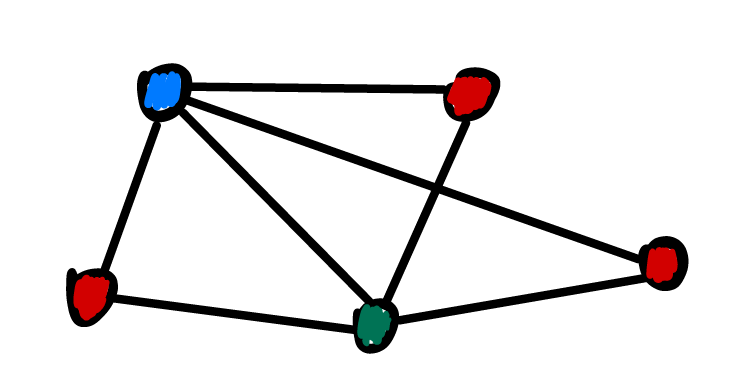
\includegraphics[width=0.4\textwidth]{images/2023-01-31/graph-coloring.png}
    \end{center}

    This can be \emph{verified} in polynomial time (we can check if such a coloring is a valid $3$-coloring), but it is computed in \textsf{NP} time.
\end{example}
\begin{definition}
    An \textsf{NP}-complete problem is a ``hardest'' problem in \textsf{NP}. Every problem in \textsf{NP} is at least as hard as an \textsf{NP}-complete problem.
\end{definition}

Right now, we assume $\mathsf{P}\neq\mathsf{NP}$. As of right now, there is no realistic algorithm that can solve any \textsf{NP} problem in polynomial-time.

Even further, we pick some problems not in $\mathsf{NP}$-complete, not in $\mathsf{P}$. We assume they are neither $\mathsf{NP}$-complete nor in $\mathsf{P}$ (we don't yet have a reduction, but we don't know if one could exist) The reasoning behind using these problems is as we have no good cryptoscheme relying solely on $\mathsf{NP}$-complete problems (we need something weaker).

\begin{center}
    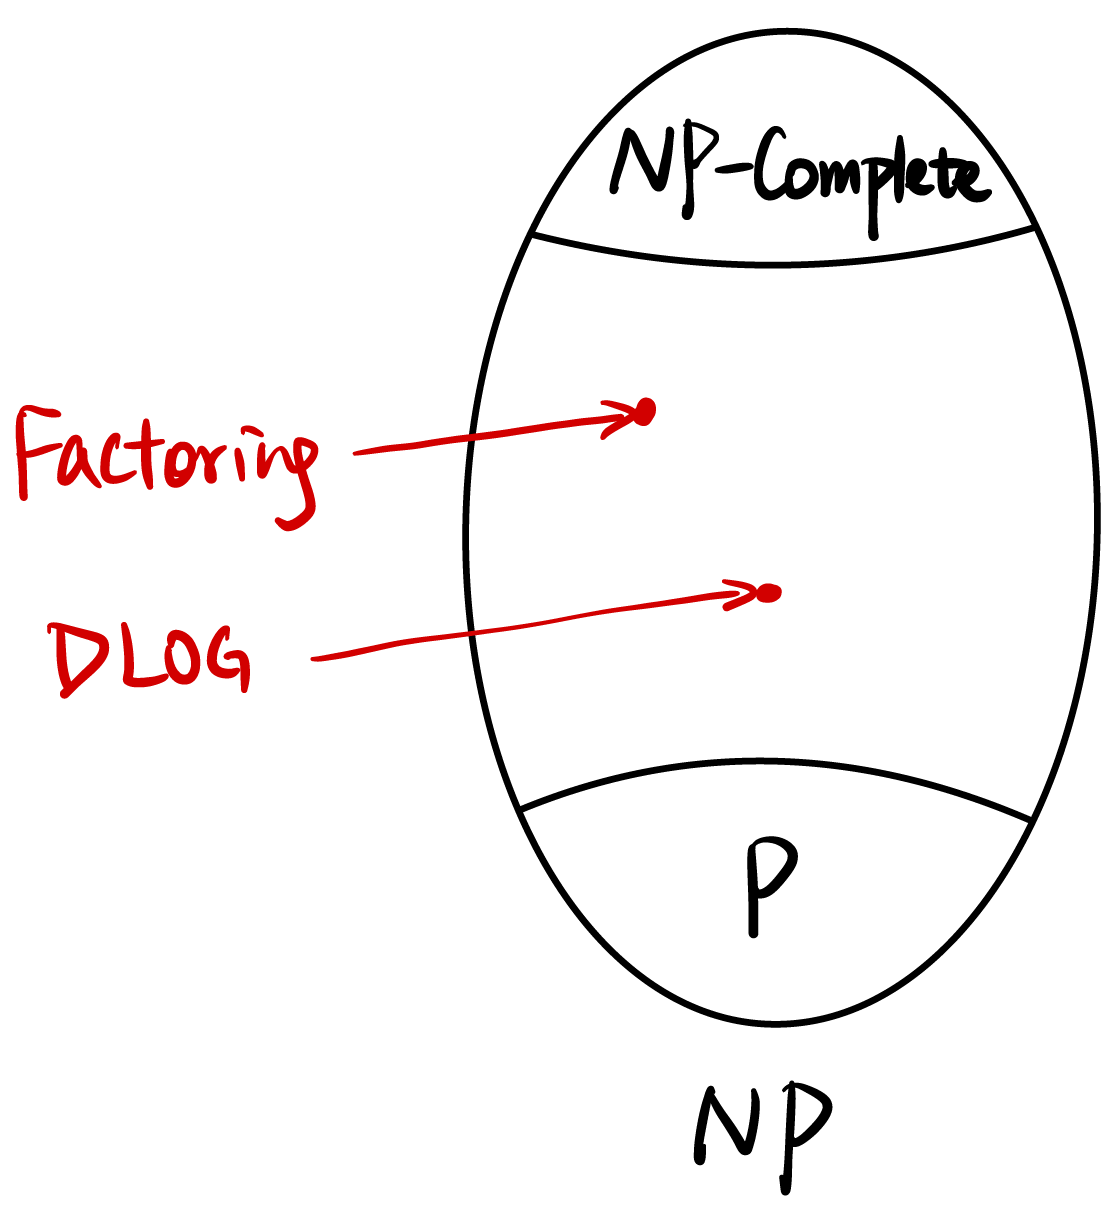
\includegraphics[width=0.4\textwidth]{images/2023-01-31/pnp-venn.png}
\end{center}

Going back to our definition of computational security \cref{def:computational-security},
\begin{definition*}[Computational Security]
    We say that the adversary is computationally bounded (is only a \emph{polynomial-time algorithm}), that $\forall \text{probabilic poly-time algorithm }\mathcal{A}$,
    \[\Enc_k(m_0)\overset{c}{\simeq}\Enc_k(m_1)\]
    Where $\overset{c}{\simeq}$ is ``computationally indistinguishable''.
\end{definition*}

What does it mean for distributions to be ``computationally indistinguishable''? Let's say Alice encrypts multiple messages $m_0, m_1, \dots$ to Bob and produces $c_0, c_1, \dots$. Even if Eve can see all plaintexts $m_i$ in the open and ciphertexts $c_i$ in the open, between known $m_0, m_1$ and randomly encrypting one of them $c\leftarrow \Enc_{k}(m_b)$ where $b\sampledfrom \{0, 1\}$, the adversary cannot determine what the random choice bit $b$ is. That is, $\Pr[b = b'] \leq \frac{1}{2} + \mathsf{negligible}(\lambda)$\footnote{$\lambda$ is the security parameter, roughly a measure of how secure the protocol is. If it were exactly equal $\frac{1}{2}$, we have information-theoretic security.}. This is Chosen-Plaintext Attack (CPA) Security.

\begin{center}
    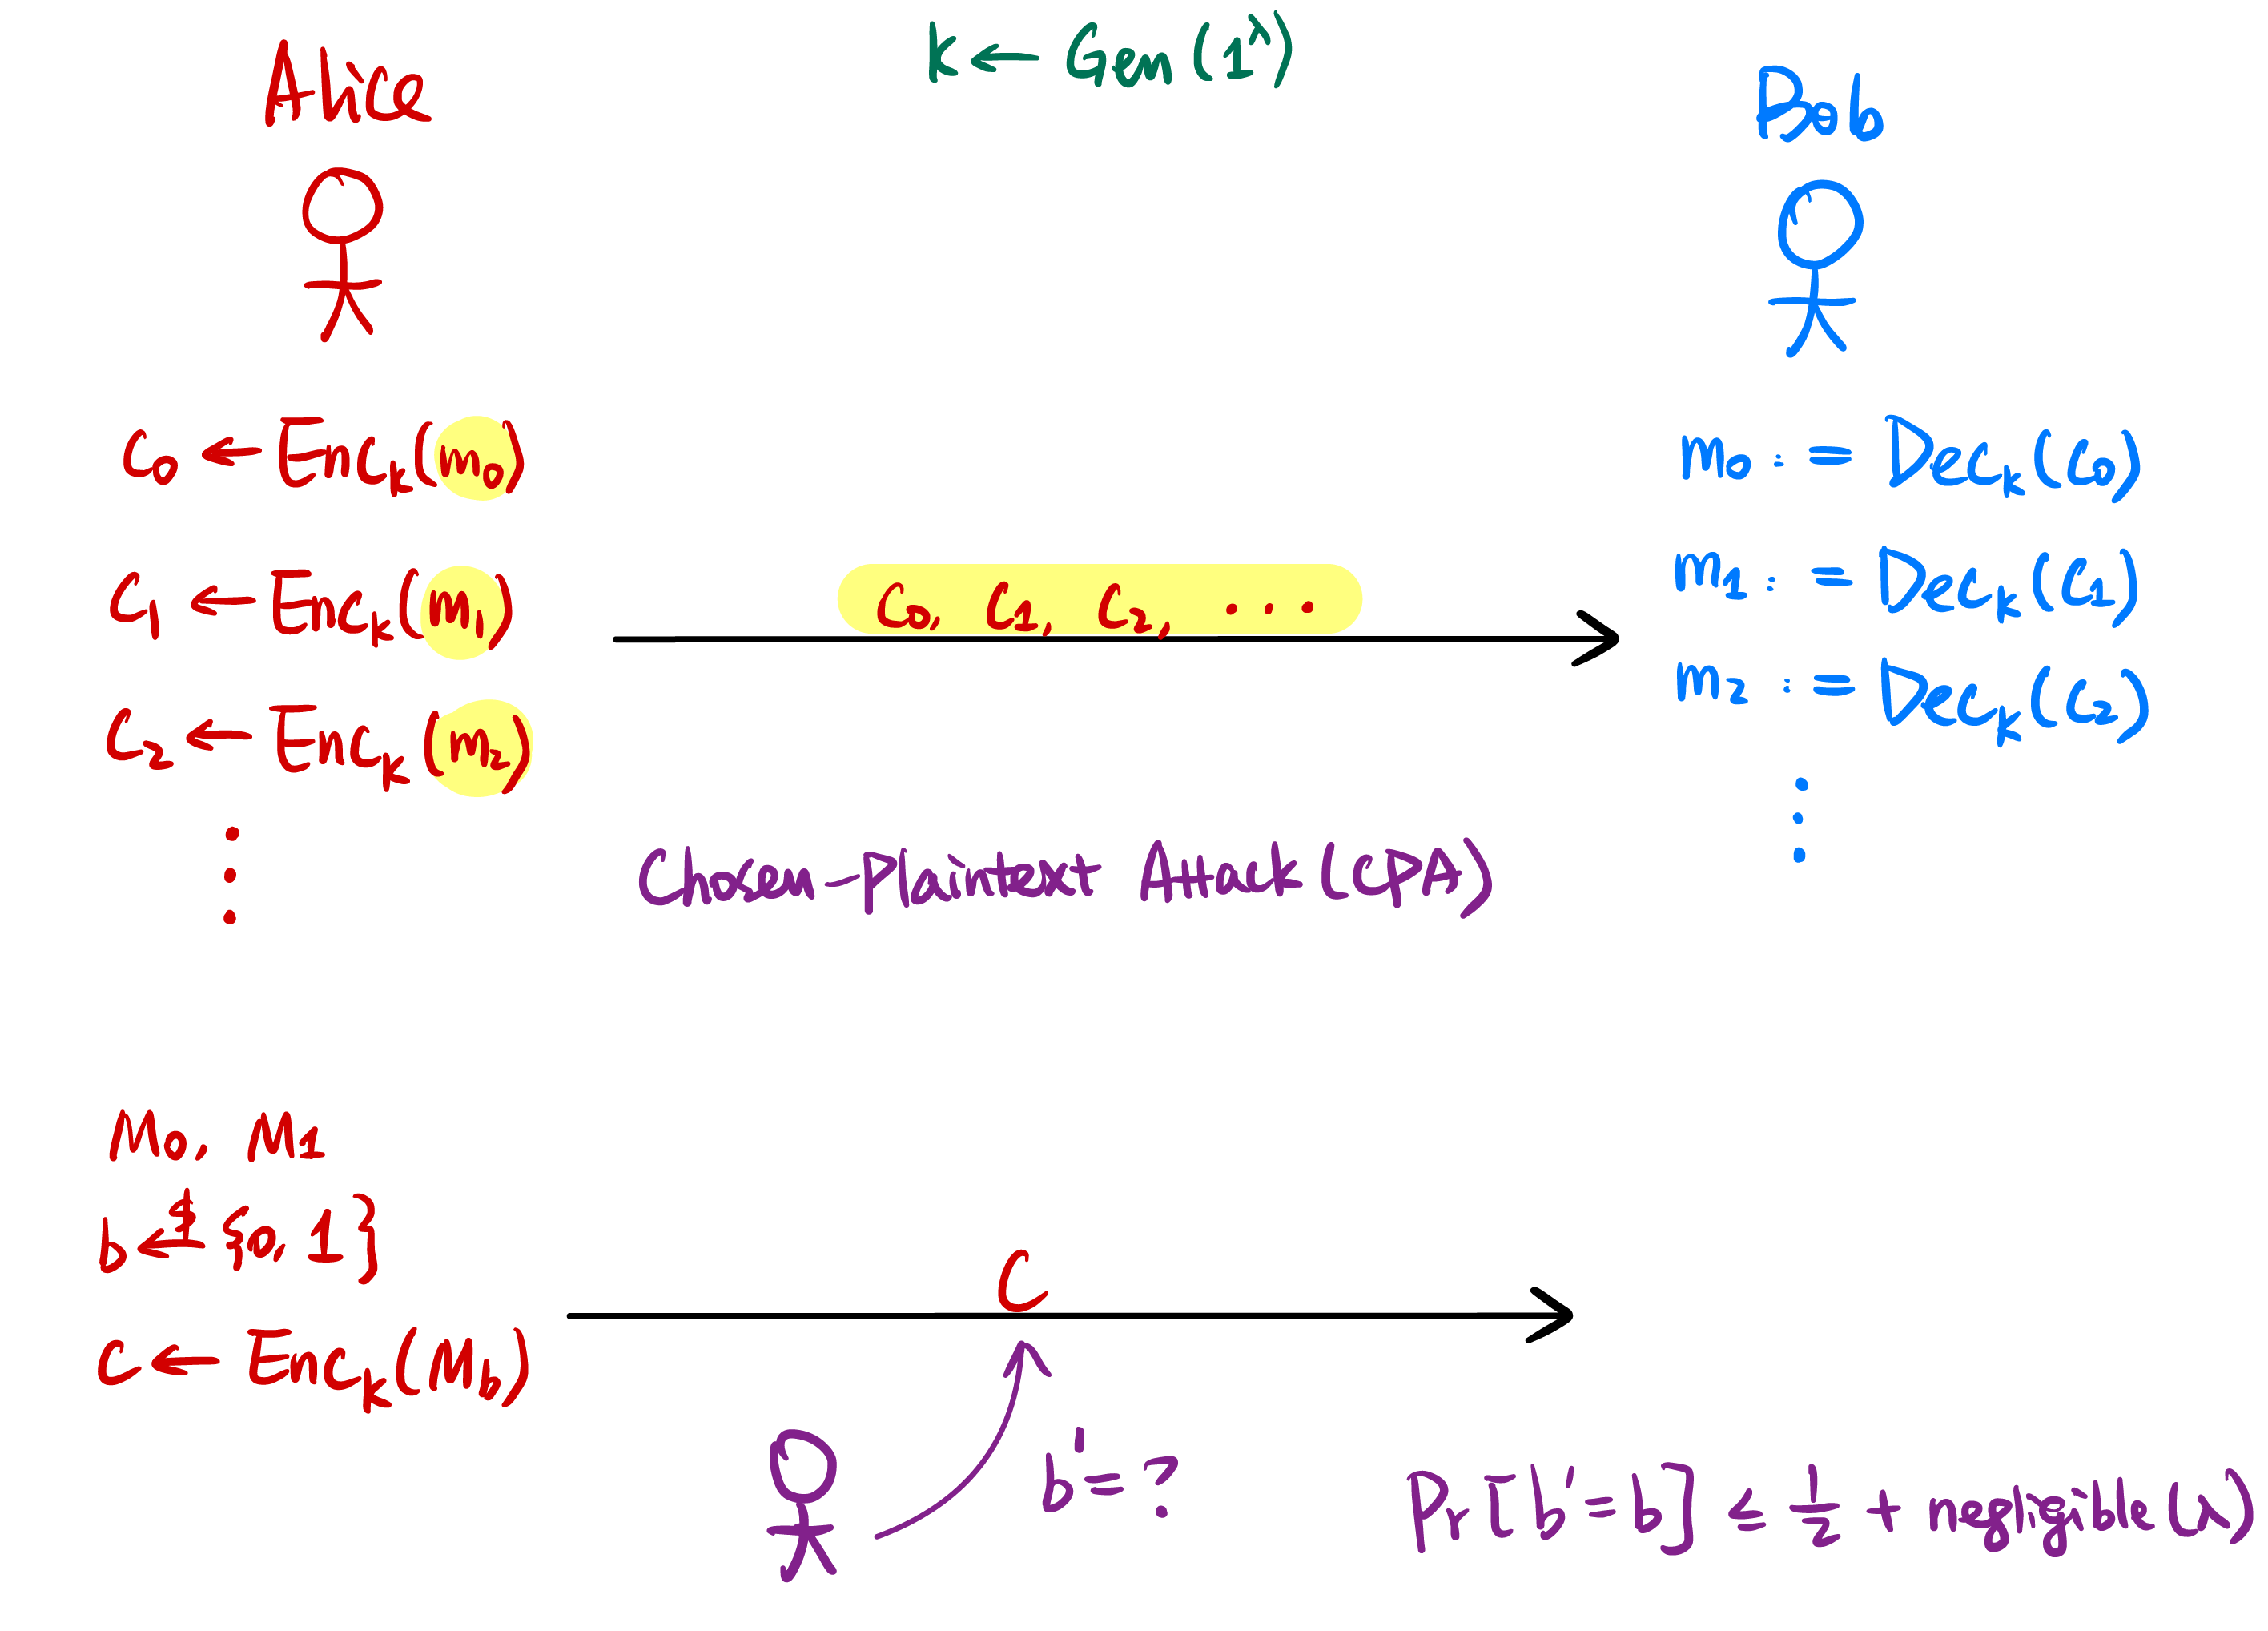
\includegraphics[width=0.8\textwidth]{images/2023-01-31/computational-security.png}
\end{center}

For a key generated $k\leftarrow \Gen(1^\lambda)$.

Theoretically, for $\lambda$ a security parameter and an adversary running in time $\mathsf{poly}(\lambda)$, the adversary should have distinguishing advantage $\negligible(\lambda)$ where
\[\negligible(\lambda) \ll \frac{1}{\lambda^c}\qquad \forall\text{ constant }c.\]

In practice, we set $\lambda = 128$. This means that the best algorithm to break the scheme (e.g. find the secret key) takes time $\sim 2^\lambda$. Currently, this is longer than the age of the universe.

\begin{example}
    \textbf{If the best algorithm is a brute-force search for $k$, what should our key length be?}

    It can just be a $\lambda$ bit string.
\end{example}
\begin{example*}
    \textbf{What if the best algorithm is no longer a brute-force search, but instead for a key length $l$ takes $\sim \sqrt{2^l}$?}

    Our key length should be $2\lambda$. Doing the math, we want $\sqrt{2^l} \equiv 2^\lambda$, solving for $l$ gives $2\lambda$.
\end{example*}

Going back to the original problem of secret-key encryption, how can we use our newfound cryptographic constructions to improve this?

From a pseudorandom function/permutation (PRF/PRP), we can reuse our secret key by passing it through the pseudorandom function.

The current practical construction for PRD/PRP is called the block cipher, and the standardized implementation is AES\footnote{Determined via a competition for such an algorithm in the early 2000s. }

It is a computational assumption\footnote{Based on heuristic, not involving any number theory!} that the AES construction is secure, and the best attack is currently a brute-force search (in both classical and quantum computing realms).

\subsubsection{Public-Key Encryption Schemes}
Using computational assumptions, we explore some public-key encryption schemes.

\begin{description}
    \item[RSA Encryption.] This is based on factoring/RSA assumption, that factoring large numbers is hard.
    \item[ElGamal Encryption.] This is based on the discrete logarithm/Diffie-Hellman Assumption, that finding discrete logs in $\ZZ_p$ is hard.
    \item[Lattice-Based Encryption.] The previous two schemes are not quantum secure. Quantum computation will break these schemes. Lattice-based encryption schemes are post-quantum secure. They are associated with the difficulty of finding `short' vectors in lattices\footnote{Covered later in class, we focus on the first two now.}.
\end{description}

Another thing worth mentioning is that
\begin{theorem}
    \emph{(Very informally,)} It is impossible to construct PKE from SKE in a black-box way. This is called ``black-box separation''.
\end{theorem}

We first need to define a bit of number-theory background.
\begin{definition}
    We denote $a\mid b$ as $a$ \ul{divides} $b$, that is, there is integer $c$ such that $b = a\cdot c$.
\end{definition}
\begin{definition}
    The $\gcd(a, b)$ is the greatest common divisor of $a, b$. If $\gcd(a, b) = 1$, then $a, b$ are coprime.
\end{definition}
\begin{ques*}
    How do we compute $\gcd$? What is its time complexity?
\end{ques*}
\begin{example*}
    We use the Euclidean Algorithm. Take $\gcd(12, 17)$,
    \begin{align*}
        17\mod{12} & = 5 \\
        12 \mod{5} & = 2 \\
        5\mod{2}   & = 1 \\
        2\mod{1}   & = 0
    \end{align*}
    or take $\gcd(12, 18)$
    \begin{align*}
        18\mod{12} & = 6 \\
        12\mod{6}  & = 0
    \end{align*}
\end{example*}
If we have two bitstrings of length $n$ bits, what is the running time of the Euclidan Algorithm?

\begin{center}
    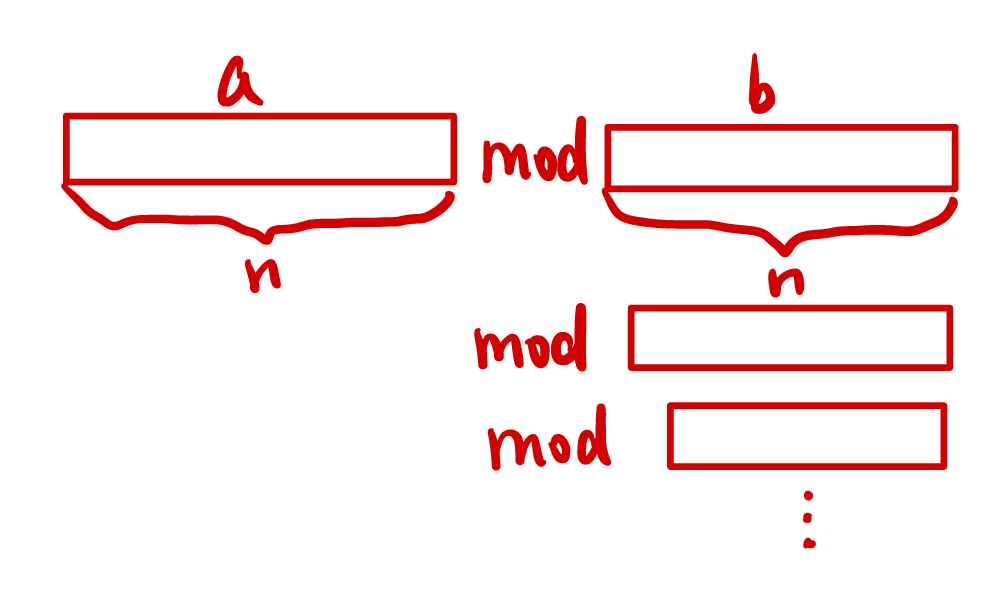
\includegraphics[width=0.3\textwidth]{images/2023-01-31/euclidean-algo.png}
\end{center}

Very informally, we see that every step, the length of $a, b$ decrease by approximately $1$ bit. Then, finding $\gcd$ is roughly order $O(n)$.

\begin{definition}[Mod]
    $a\mod{N}$ is the remainder of $a$ when divided by $N$.

    $a\equiv b\pmod{N}$ means when $a$ and $b$ are \ul{congruent modulo} $N$. That is, $a\mod N = b\mod N$.
\end{definition}

\begin{ques*}
    How might we compute $a^b\mod N$? What is the time complexity? Let $a, b, N$ be $n$-bit strings.
\end{ques*}

Na\"ively, we can repeatedly multiply. But this takes $b$ steps ($2^n$).

We can `repeatedly square'. For example, we can get to $a^8$ faster by getting $a^2$, squaring to get $a^4$, and again to get $a^8$. We can take the bitstring of $b$ and determine how to compute this.

\begin{example*}
    If $b = 100101_2$, we take $a\cdot a^4\cdot a^{32}\mod N$ which can be calculated recursively (an example is given in the first assignment).
\end{example*}

The time complexity of this is order $O(n)$ for $n$-bit $a, b, N$\footnote{Not exactly order $n$, we should add the complexity of multiplication. However, this should be bounded by $N$ since we can log at every step.}.

\begin{theorem}[Bezout's Theorem, \emph{roughly}]
    If $\gcd(a,N) = 1$, then $\exists b$ such that
    \[a\cdot b \equiv 1\pmod{N}.\]
    This is to say, $a$ is \ul{invertible modulo} $N$. $b$ is its inverse, denoted as $a^{-1}$.
\end{theorem}
\begin{ques*}
    How do we compute $b$?
\end{ques*}
We can use the Extended Euclidean Algorithm!
\begin{example*}
    We write linear equations of $a$ and $N$ that sum to $1$, using our previous Euclidean Algorithm. Take the previous example $\gcd(12, 17)$,
    \begin{align*}
        17\mod{12} & = 5 \\
        12 \mod{5} & = 2 \\
        5\mod{2}   & = 1 \\
        2\mod{1}   & = 0
    \end{align*}
    We write this as
    \begin{align*}
        5 & = 17 - 12\cdot 1                         \\
        2 & = 12 - 5\cdot 2 = 12\cdot x + 17\cdot y  \\
        1 & = 5 - 2\cdot 2 = 12\cdot x' + 17\cdot y'
    \end{align*}
    where we substitute the linear combination of $5$ into $5$ on line $2$, substitute linear combination of $2$ into $2$ on line $1$, each producing another linear combination of $12, 17$.

    If $\gcd(a, N) = 1$, we use the Extended Euclidean Algorithm to write $1 = a\cdot x + N\cdot y$, then $1\equiv a\cdot x\pmod{N}$.
\end{example*}

\begin{definition}[Group of Units mod $N$]
    We have set
    \[\ZZ_N^\times:= \left\{ a\mid a\in [1, N-1], \gcd(a, N) = 1 \right\}\]
    which is the group of units modulo $N$ (they are units since they all have an inverse by above).
\end{definition}
\begin{definition}[Euler's Phi Function]
    Euler's phi (or totient) function, $\phi(N)$, counts the number of elements in this set. That is, $\phi(N) =  |\ZZ_N^\times|$.
\end{definition}
\begin{theorem}[Euler's Theorem]
    For all $a, N$ where $\gcd(a, N) = 1$, we have that \[a^{\phi(N)} \equiv 1\pmod{N}.\]
\end{theorem}

With this, we can start talking about RSA.

\subsubsection{RSA}
We first define the RSA assumption.
\begin{definition}[Factoring Assumption]
    Given two $n$-bit primes $p, q$, we compute $N = p\cdot q$. Given $N$, it's computationally hard to find $p$ and $q$ (classically).
\end{definition}
\begin{definition}[RSA Assumption]
    Given two $n$-bit primes, we again compute $N = p\cdot q$, where $\phi(N) = (p-1)(q-1)$. We choose an $e$ such that $\gcd(e, \phi(N)) = 1$ and compute $d \equiv e^{-1}\pmod{\phi(N)}$.

    Given $N$ and a random $y\sampledfrom \ZZ_{N}^\times$, it's computationally hard to find $x$ such that $x^e\equiv y\pmod{N}$.

    \begin{center}
        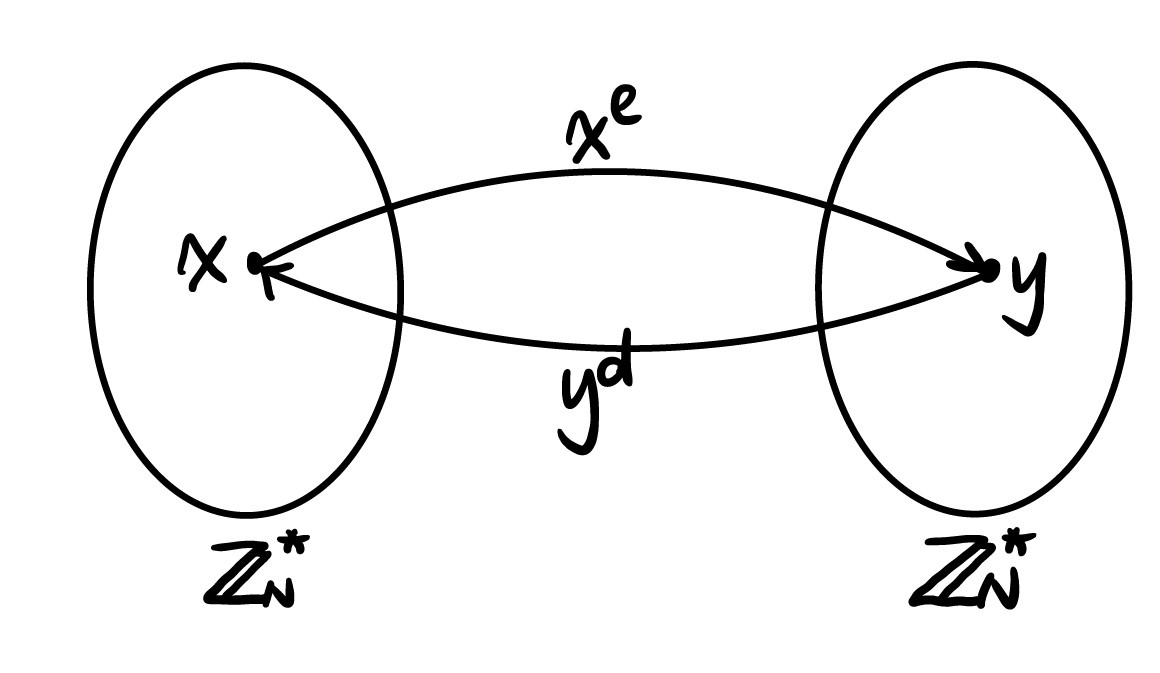
\includegraphics[width=0.4\textwidth]{images/2023-01-31/rsa.png}
    \end{center}

    However, given $p, q$, it's easy to find $d$. We know $\phi(N) = (p-1)(q-1)$, so we can compute $d$ from $e$ by running the Extended Euclidean Algorithm. Then, taking $(x^e)^d\equiv x^{ed}\equiv x$ which allows us to extract $x$ again.
\end{definition}

Encrypting is exactly raising by power $d$, and decrypting is raising again by power $e$.

Remaining questions:
\begin{itemize}
    \item How can we generate primes $p, q$?
    \item How can we pick $e$ such that $\gcd(e, \phi(N)) = 1$?
    \item What security issues can you see?
\end{itemize}

We'll continue next class.
%!TEX root = ../notes.tex
\section{January 31, 2024}
\label{20240131}
\subsection{RSA Encryption, \emph{continued}}
\recall that the RSA encryption algorithm contains 3 components:
\begin{description}
    \item[$\Gen(1^\lambda)$:] Generate two $n$-bit primes $p, q$. We compute $N = p\cdot q$ and $\phi(N) = (p-1)(q-1)$. Choose $e$ such that $gcd(e, \phi(N)) = 1$. We compute $d = e^{-1}\mod{\phi(N)}$. Our public key $pk = (N, e)$, our secret key is $sk = d$.
    \item[$\Enc_{pk}(m)$:] $c = m^e\mod{N}$.
    \item[$\Dec_{sk}(c)$:] $m = c^d\mod{N}$.
\end{description}
We have a few remaining questions:
\begin{enumerate}
    \item How do we generate 2 primes $p, q$?
    \item How do we choose such an $e$?
    \item How do we compute $d = e^{-1}\mod{\phi(N)}$?
    \item How do we efficiently compute $m^e\mod{N}$ and $c^d\mod N$.
\end{enumerate}
How do we resolve these issues to ensure the $\Gen$ step is efficient (polynomial time).
\begin{enumerate}
    \item We pick an arbitrary number $p$ and check for primality efficiently (using Miller Rabin, a probabilistic primality test). We pick random numbers until they are prime. Since primes are `pretty dense' in the integers, this can be done efficiently.
    \item We can also guess! Since we're unsure whether coprime numbers are dense, we can pick small prime $e$.
    \item We can compute $d$ using the Extended Euclidean Algorithm.
    \item We can repeatedly square (using fast power algorithm).
\end{enumerate}

\begin{ques*}
    What happens if we can factor?
\end{ques*}
    
A note that we have correctness with this scheme: $(m^e)^d= m^{ed} = m\mod N$.

\begin{ques*}
    Still, are there any security issues?
\end{ques*}
\begin{itemize}
    \item It relies on factoring being difficult (this is the computational assumption). Post-quantum, Shor's Algorithm will break RSA.
    \item Recall last lecture that CPA (Chosen-Plaintext Attack) security was defined as an adversary not being able to discern between an encryption of $m_0$ and $m_1$, \emph{knowing} $m_0$ and $m_1$ in the clear.

          Eve could just encrypt $m_0$ and $m_1$ themselves using public $e$, and discern which of the plaintexts the ciphertext corresponds to. Using RSA, you \emph{really} have to be careful. For RSA, this is a very concrete attack.

          The concrete reason is that the encryption algorithm $\Enc$ is \emph{deterministic}. If you encrypt the same message twice, it will be the same ciphertext. We really want to be sure that $m\sampledfrom \ZZ_N^\times$ (that it has enough entropy).

          Returning on the RSA assumption. It's crucial that the $y\sampledfrom \ZZ_N^\times$ is randomly sampled.
\end{itemize}

\begin{ques*}
    In practice, how can RSA be useful with these limitations?
\end{ques*}

As long as we pick the plaintext which is randomly sampled, security for RSA holds.

\begin{remark*}
    In practice, we usually set length of $p$ and $q$ to be $1024$ bits, and the key length is $2048$ bits. This is because of better algorithms for finding big primes.
\end{remark*}

\begin{ques*}
    Asked on \href{https://edstem.org/us/courses/33693/discussion/2483699}{Ed}: What happens if $p\mid m$ (or $q\mid m$)?
\end{ques*}

Correctness still holds\footnote{Can do out, or by using Chinese Remainder Theorem to see that it preserves the qualities we need mod $p$ and mod $q$. }.

However, security will be broken. If $p\mid (m^2\mod N)$, then $gcd(c, N) = p$ will factor $N$.

However, this is \emph{very} unlikely! Sampling $m\sampledfrom [1, N-1]$, then
\[\Pr[p\mid m] \equiv \frac{q}{N} = \frac{1}{p} = \frac{1}{2^{\theta(\lambda)}}=\negligible(\lambda)\]

When sending $k$ messages,
\[\Pr[p\mid m\text{ for any }m] \leq \frac{k}{p} \equiv \frac{\mathsf{poly}(\lambda)}{2^{\theta(\lambda)}}\]

which is still negligible. Put simply, Alice has just as much chance to break RSA by randomly factoring as she is to send a message that is a multiple of $p$ or $q$.

\subsection{Intro to Group Theory}
\begin{definition}[Group]
    A \ul{group} is a set $\GG$ along with a binary operation $\circ$ with properties:
    \begin{description}
        \item[Closure.] $\forall g, h\in \GG$, $g\circ h\in \GG$.
        \item[Existence of an identity.] $\exists e\in \GG$ such that $\forall g\in \GG$, $e\circ g = g\circ e = g$.
        \item[Existence of inverse.] $\forall g\in \GG$, $\exists h\in \GG$ such that $g\circ h = h\circ g = e$. We denote the inverse of $g$ as $g^{-1}$.
        \item[Associativity.] $\forall g_1, g_2, g_3\in \GG$, $(g_1\circ g_2)\circ g_3 = g_1\circ(g_2\circ g_3)$.
    \end{description}

    We say a group is additionally \emph{Abelian} if it satisfies
    \begin{description}
        \item[Commutativity.] $\forall g, h\in \GG$, $g\circ h = h \circ g$.
    \end{description}
    For a finite group, we use $|\GG|$ to denote its \emph{order}.
\end{definition}
\begin{example}
    $(\ZZ, +)$ is an Abelian group.

    We can check so: two integers sum to an integer, identity is $0$, the inverse of $a$ is $-a$, addition is associative and commutative.

    $(\ZZ, \cdot)$ is not a group.

    $(\ZZ_N^\times, \cdot)$ is an Abelian group ($\cdot$ is multiplication mod $N$).
\end{example}

\begin{definition}[Cyclic Group]
    Let $\GG$ be a group of order $m$. We denote
    \[\langle g\rangle := \{e=g^0, g^1, g^2, \dots, g^{m-1}\}.\]
    $\GG$ is a \ul{cyclic group} if $\exists g\in \GG$ such that $\langle g\rangle = \GG$. $g$ is called a \ul{generator} of $\GG$.
\end{definition}

\begin{example*}
    $\ZZ_p^\times$ (for prime $p$) is a cyclic group of order $p-1$\framedfootnote{A proof of this extends beyond the scope of this course, but you are recommended to check out Math 1560 (Number Theory) or Math 1580 (Cryptography). You can take this on good faith. }.
    \[\ZZ_7^\times = \{3^0 = 1, 3^1, 3^2=2, 3^3 = 6, 3^4 = 5, 3^5 = 5\}.\]
\end{example*}
\begin{ques*}
    How do we find a generator?
\end{ques*}
For every element, we can continue taking powers until $g^\alpha = 1$ for some $\alpha$. We hope that $\alpha = p-1$ (the order of $g$ is the order of the group), but we know at least $\alpha \mid p-1$.

\subsection{Computational Assumptions}

We have a few assumptions we make called the Diffie-Hellman Assumptions, in order of \textbf{weakest to strongest}\footnote{If one can solve DLOG, we can solve CDH. Given CDH, we can solve DDH. This is why CDH is \emph{stronger} than DDH, and DDH is \emph{stronger} than DLOG. It's not necessarily true the other way around (similar to factoring and DSA assumptions). } assumptions.

Let $(\GG, q, g)\leftarrow \mathcal{G}(1^\lambda)$ be a cyclic group $\GG$ or order $q$ (a $\theta(\lambda)$-bit integer) with generator $g$. For integer groups, keys are usually 2048-bits. For elliptic curve groups, keys are usually 256-bits.

\begin{definition}[Discrete Lgoarithm (DLOG) Assumption]
    Let $x\sampledfrom \ZZ_q$. We compute $h = g^x$.

    Given $(\GG, q, g, h)$, it's computationally hard to find the exponent $x$ (classically).
\end{definition}

\begin{definition}[Computational Diffie-Hellman (CDH) Assumption]
    $x, y\sampledfrom \ZZ_q$, compute $h_1 = g^x$, $h_2 = g^y$.

    Given $(\GG, q, g, h_1, h_2)$, it's computationally hard to find $g^{xy}$.
\end{definition}

\begin{definition}[Decisional Diffie-Hellman (DDH) Assumption]
    $x, y, z\sampledfrom \ZZ_q$. Compute $h_1 = g^x$, $h_2 = g^y$.

    Given $(\GG, q, g, h_1, h_2)$, it's computationally hard to distinguish between $g^{xy}$ and $g^z$.
    \[(g^x, g^y, g^{xy}) \csimeq (g^x, g^y, g^z).\]
\end{definition}

\subsection{ElGamal Encryption}
The ElGamal encryption scheme involves the following:
\begin{description}
    \item[$\Gen(1^\lambda)$:] We generate a group $(\GG, q, g) \leftarrow \mathcal{G}(1^\lambda)$. We sample $x\sampledfrom \ZZ_q$, compute $h = g^x$. Our public key is $pk = (\GG, q, g, h)$, secret key $sk = x$.
    \item[$\Enc_{pk}(m)$:] We have $m\in\GG$. We sample $y\sampledfrom \ZZ_q$. Our ciphertext is $c = \langle g^y, h^y\cdot m\rangle$. Note that $h = g^x$, so $g^{xy}\csimeq g^z$ is a one-time pad for our message $m$.
    \item[$\Dec_{sk}(c)$:] To decrypt $c = \langle c_1, c_2\rangle$, we raise
        \begin{align*}
            c_1^x & = (g^y)^x = g^{xy}                                      \\
            m     & = \frac{g^{xy}\cdot m}{g^{xy}} = c_2\cdot (c_1^x)^{-1}.
        \end{align*}
\end{description}

Notes about ElGamal:
\begin{itemize}
    \item Our group can be reused! We can use a public group that is fixed. In fact, there are \emph{popular} groups out there used in practice. Some of these are Elliptic Curve groups which are much more efficient than integer groups. You don't need to use the details, yet you can use it! You can use any group, so long as the group satisfies the DDH assumption.
    \item Similar to RSA, this is breakable post-quantum. Given Shor's Algorithm, we can break discrete log.
\end{itemize}

\subsection{Secure Key Exchange}
Using DDH, we can construct something very important, \emph{secure key exchange}.
\begin{definition}[Secure Key Exchange]
    Alice and Bob sends messages back and forth, and at the end of the protocol, can agree on a shared key.

    An eavesdropper looking at said communications cannot figure out what shared key they came up with.
\end{definition}
\begin{theorem}
    \emph{Informally,} It's impossible to construct secure key exchange from secret-key encryption in a black-box way.
\end{theorem}

\begin{ques*}
    How do we build a key exchange from public-key encryption?
\end{ques*}
Bob generates a keypair $(pk, sk)$. Alice generates a shared key $k\sampledfrom \{0, 1\}^\lambda$, and sends $\Enc_{pk}(k)$ to Bob.

Using Diffie-Hellman, it's very easy. We have group $(\GG, q, g)\leftarrow \mathcal{G}(1^\lambda)$. Alice samples $x\sampledfrom \ZZ_q$ and sends $g^x$. Bob also samples $y\sampledfrom \ZZ_q$ and sends $g^y$. Both Alice and Bob compute $g^{xy} = (g^x)^y = (g^y)^x$.

\begin{center}
    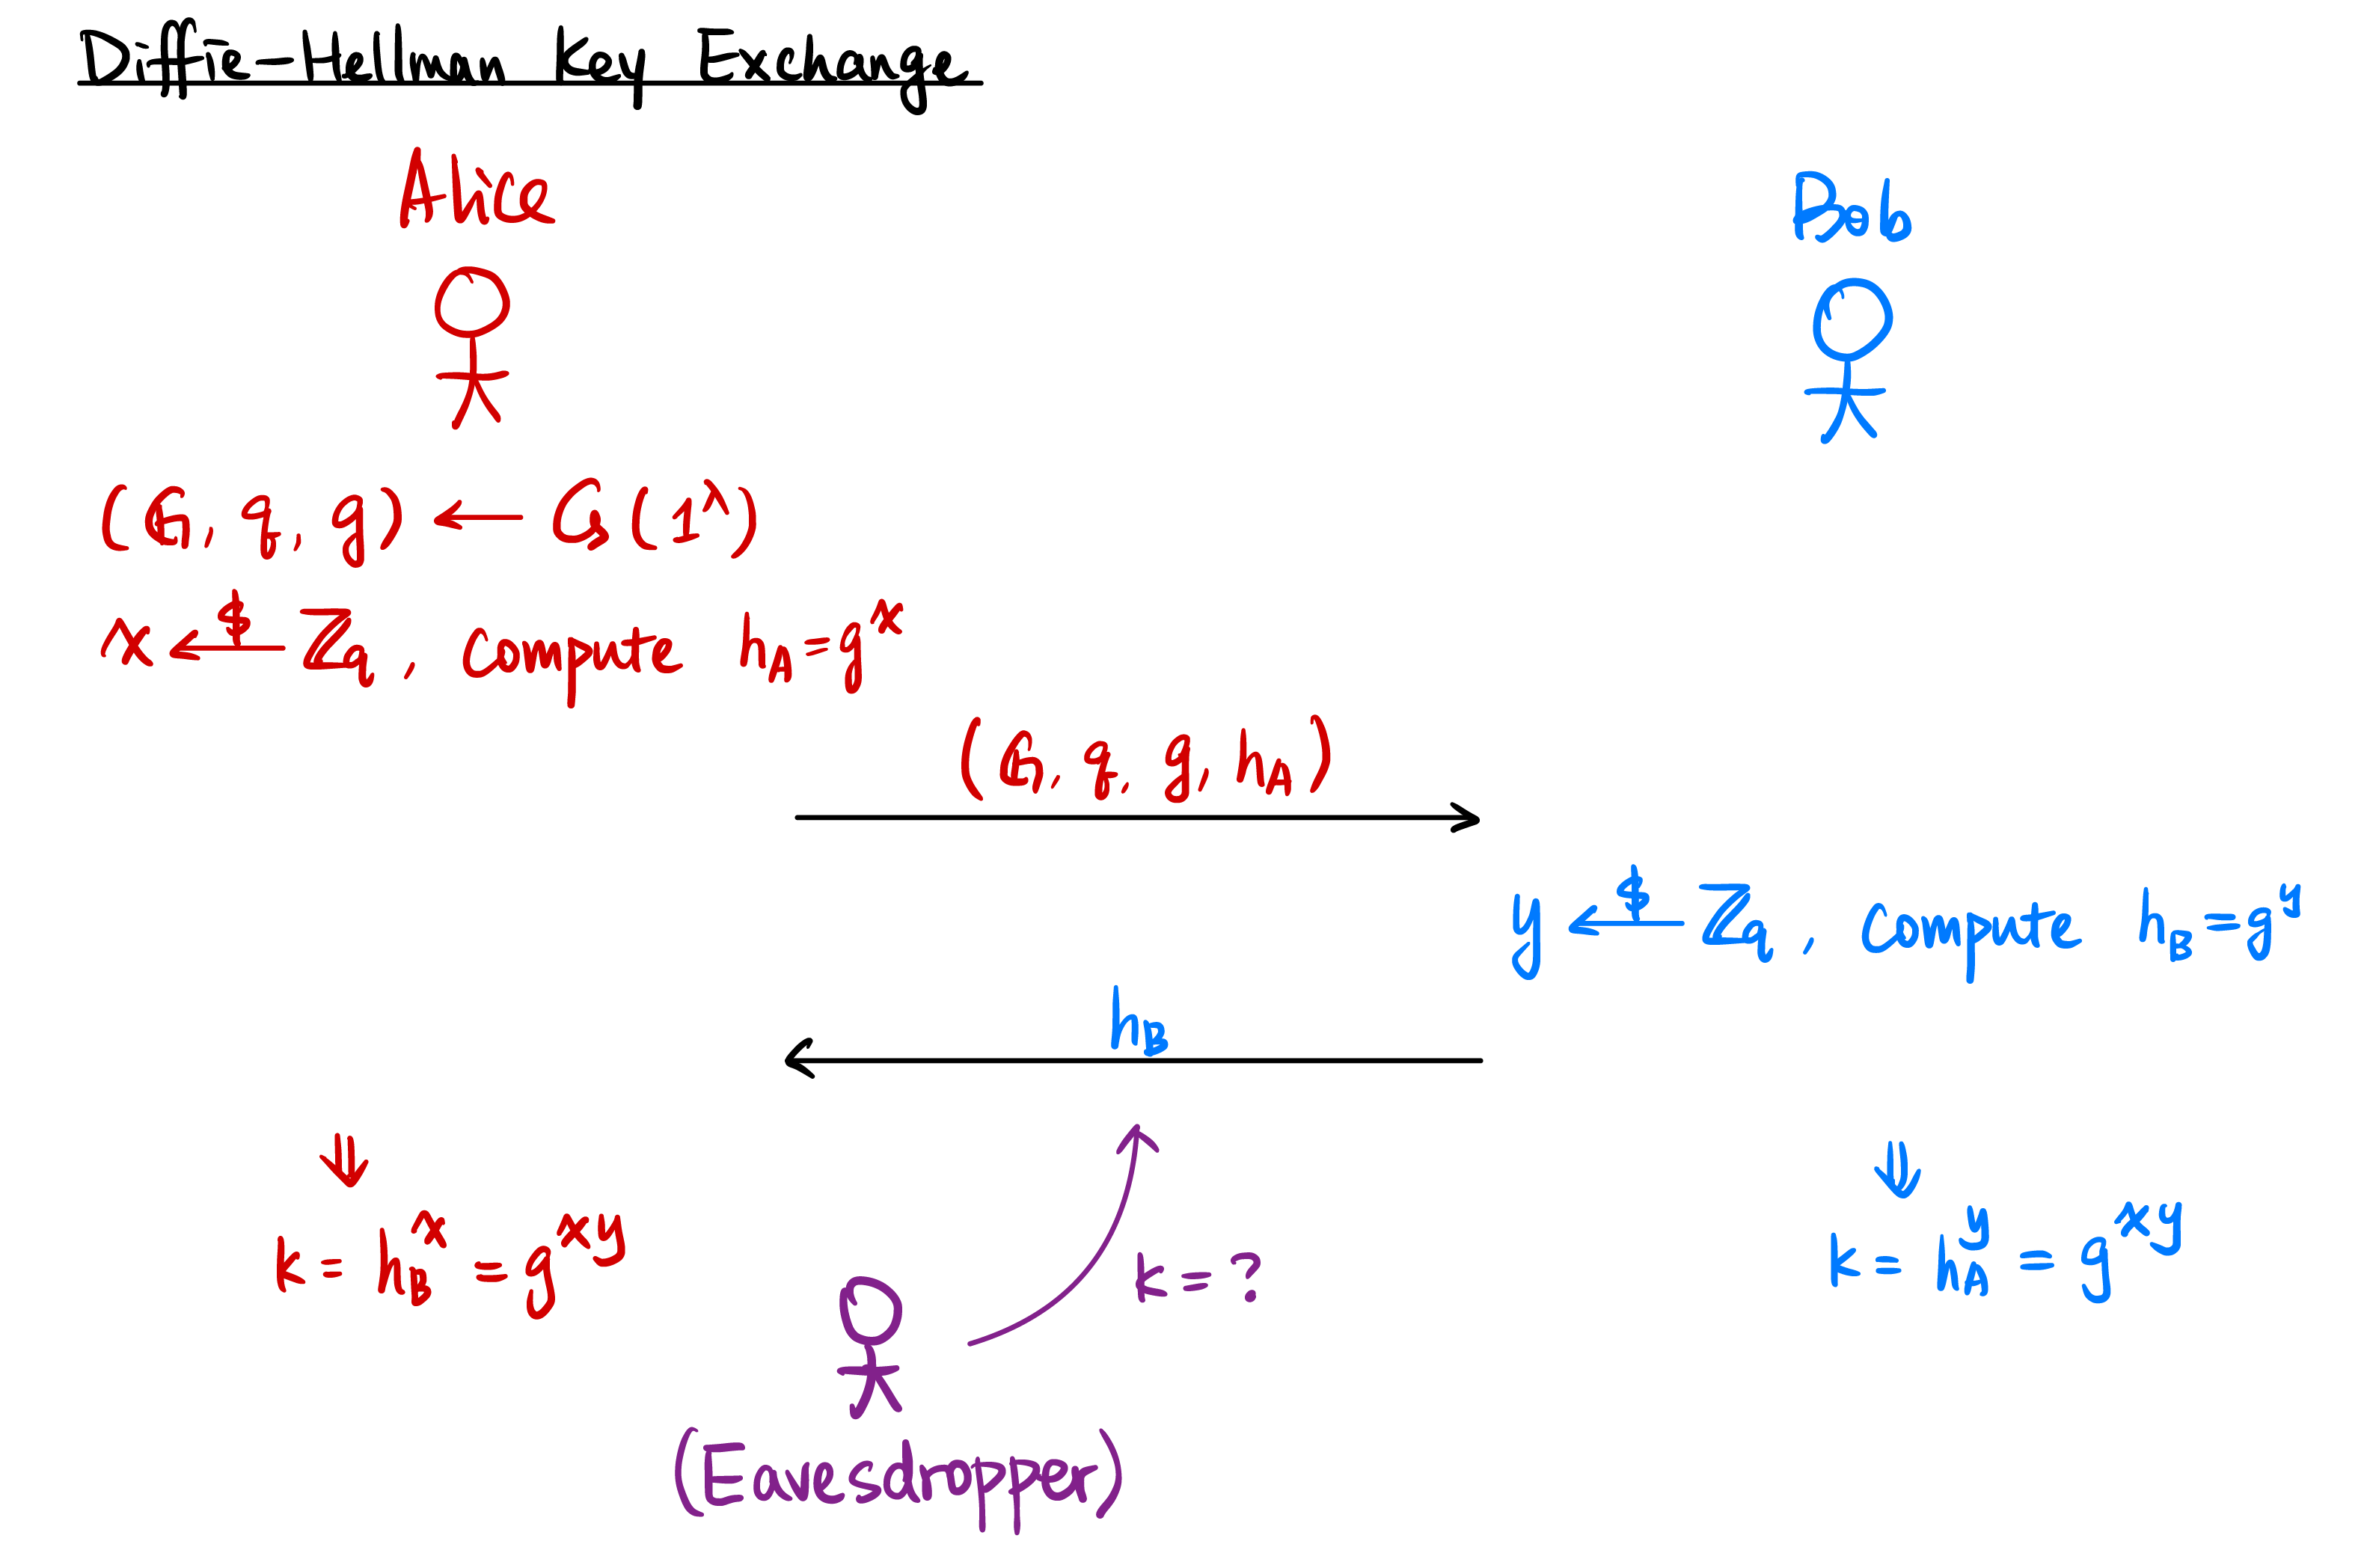
\includegraphics[width=0.8\textwidth]{images/2023-02-02/diffie-hellman.png}
\end{center}

What happens in practice is that parties run Diffie-Hellman key exchange to agree on a shared key. Using that shared key, they run symmetric-key encryption. This gives us efficiency. Additionally, private-key encryptions don't rely on heavy assumptions on the security of protocols (such as the DDH, RSA assumptions).

\subsection{Message Integrity}
Alice sends a message to Bob, how does Bob ensure that the message came from Alice?

\begin{center}
    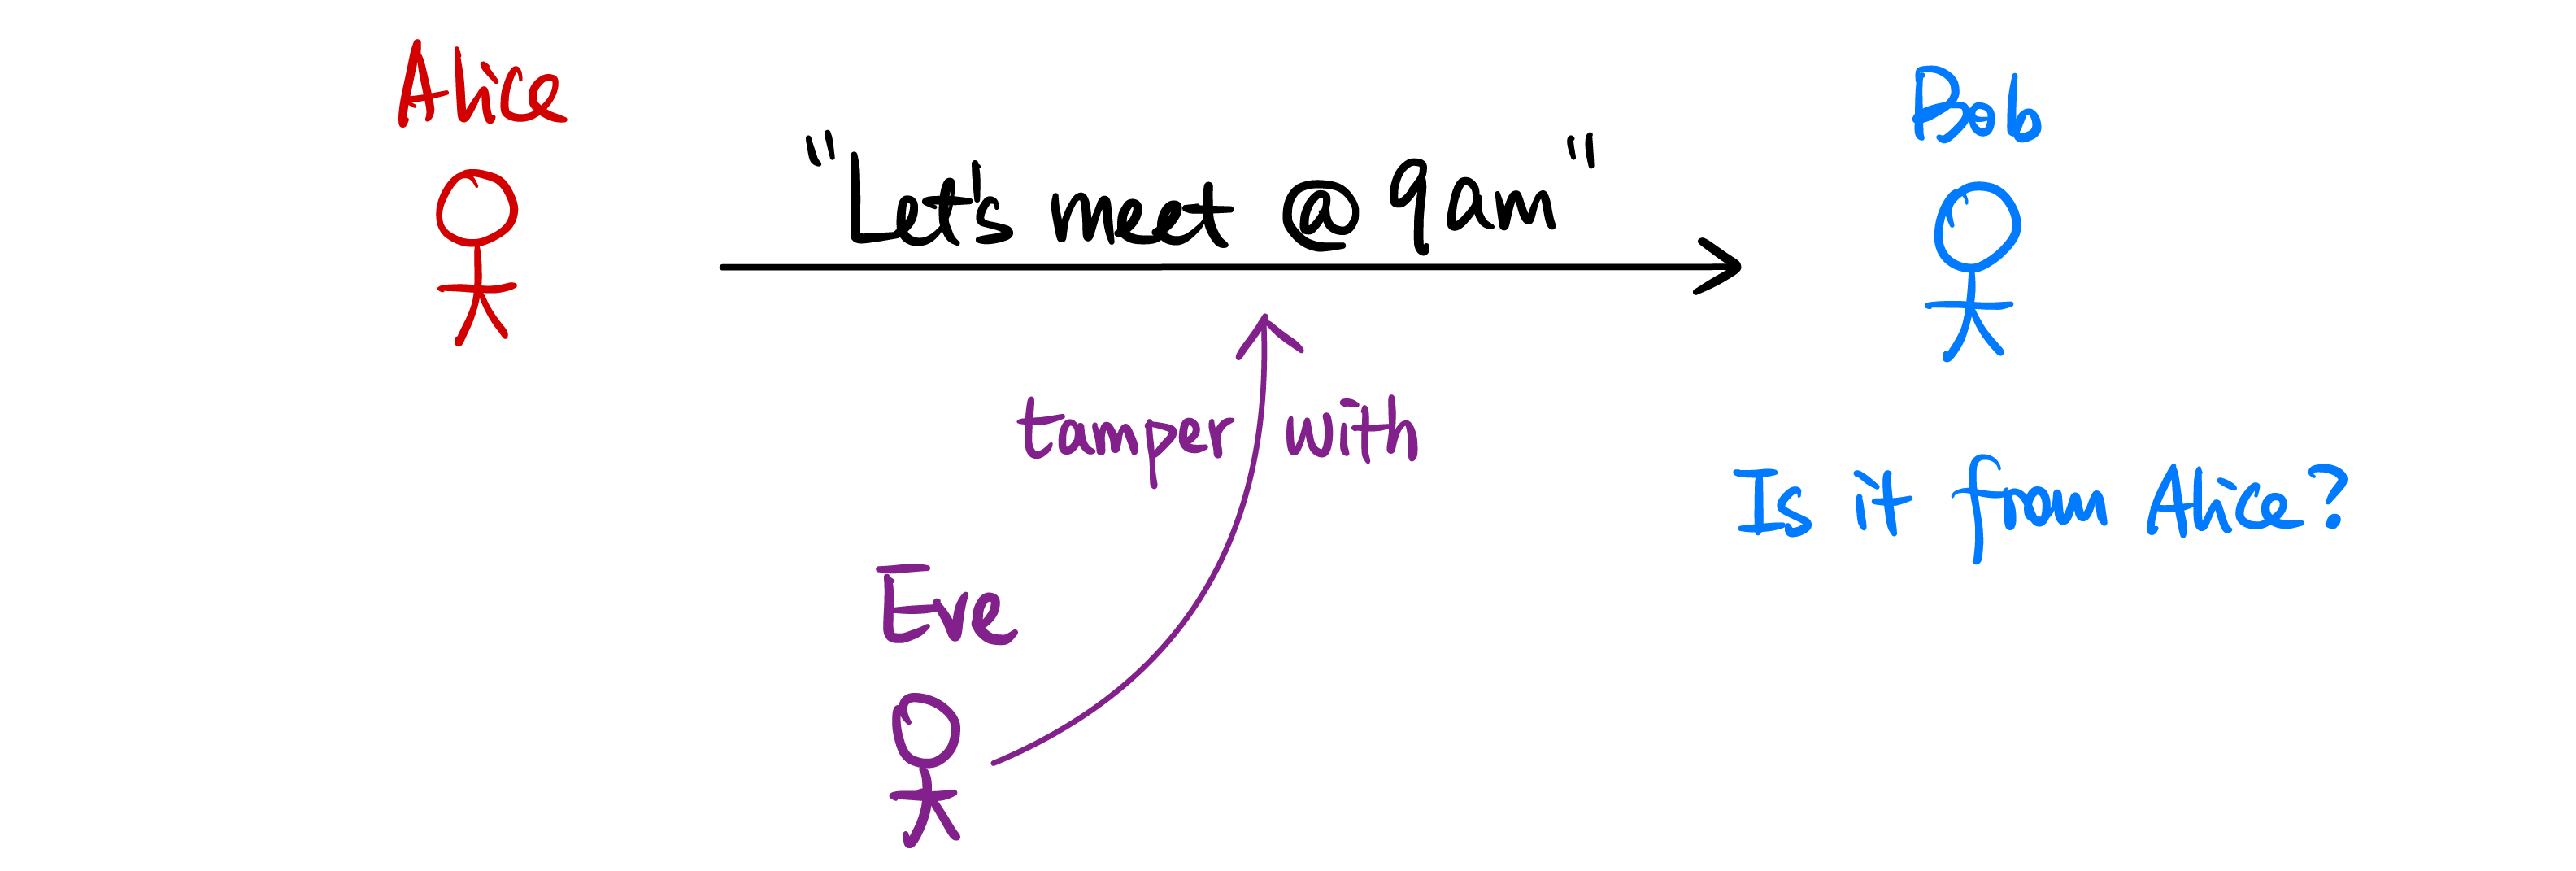
\includegraphics[width=0.8\textwidth]{images/2023-02-02/integrity.png}
\end{center}

We can build up another line of protocols to ensure message integrity. It's similar to encryption, but the parties run 2 algorithms: \emph{Authenticate} and \emph{Verify}.

Using a message $m$, Alice can generate a \emph{tag} or \emph{signature}, and Bob can verify $(m, t)$ is either valid or invalid.

Our adversary has been upgraded to an Eve who can now tamper with messages.

Similarly to encryption, we have symmetric-key and public-key encryption.

Using a shared key $k$, Alice can authenticate $m$ using $k$ to get a tag $k$. Similarly, Bob can verify whether $(m, t)$ is valid using $k$. This is called a Message Authentication Code.

\begin{center}
    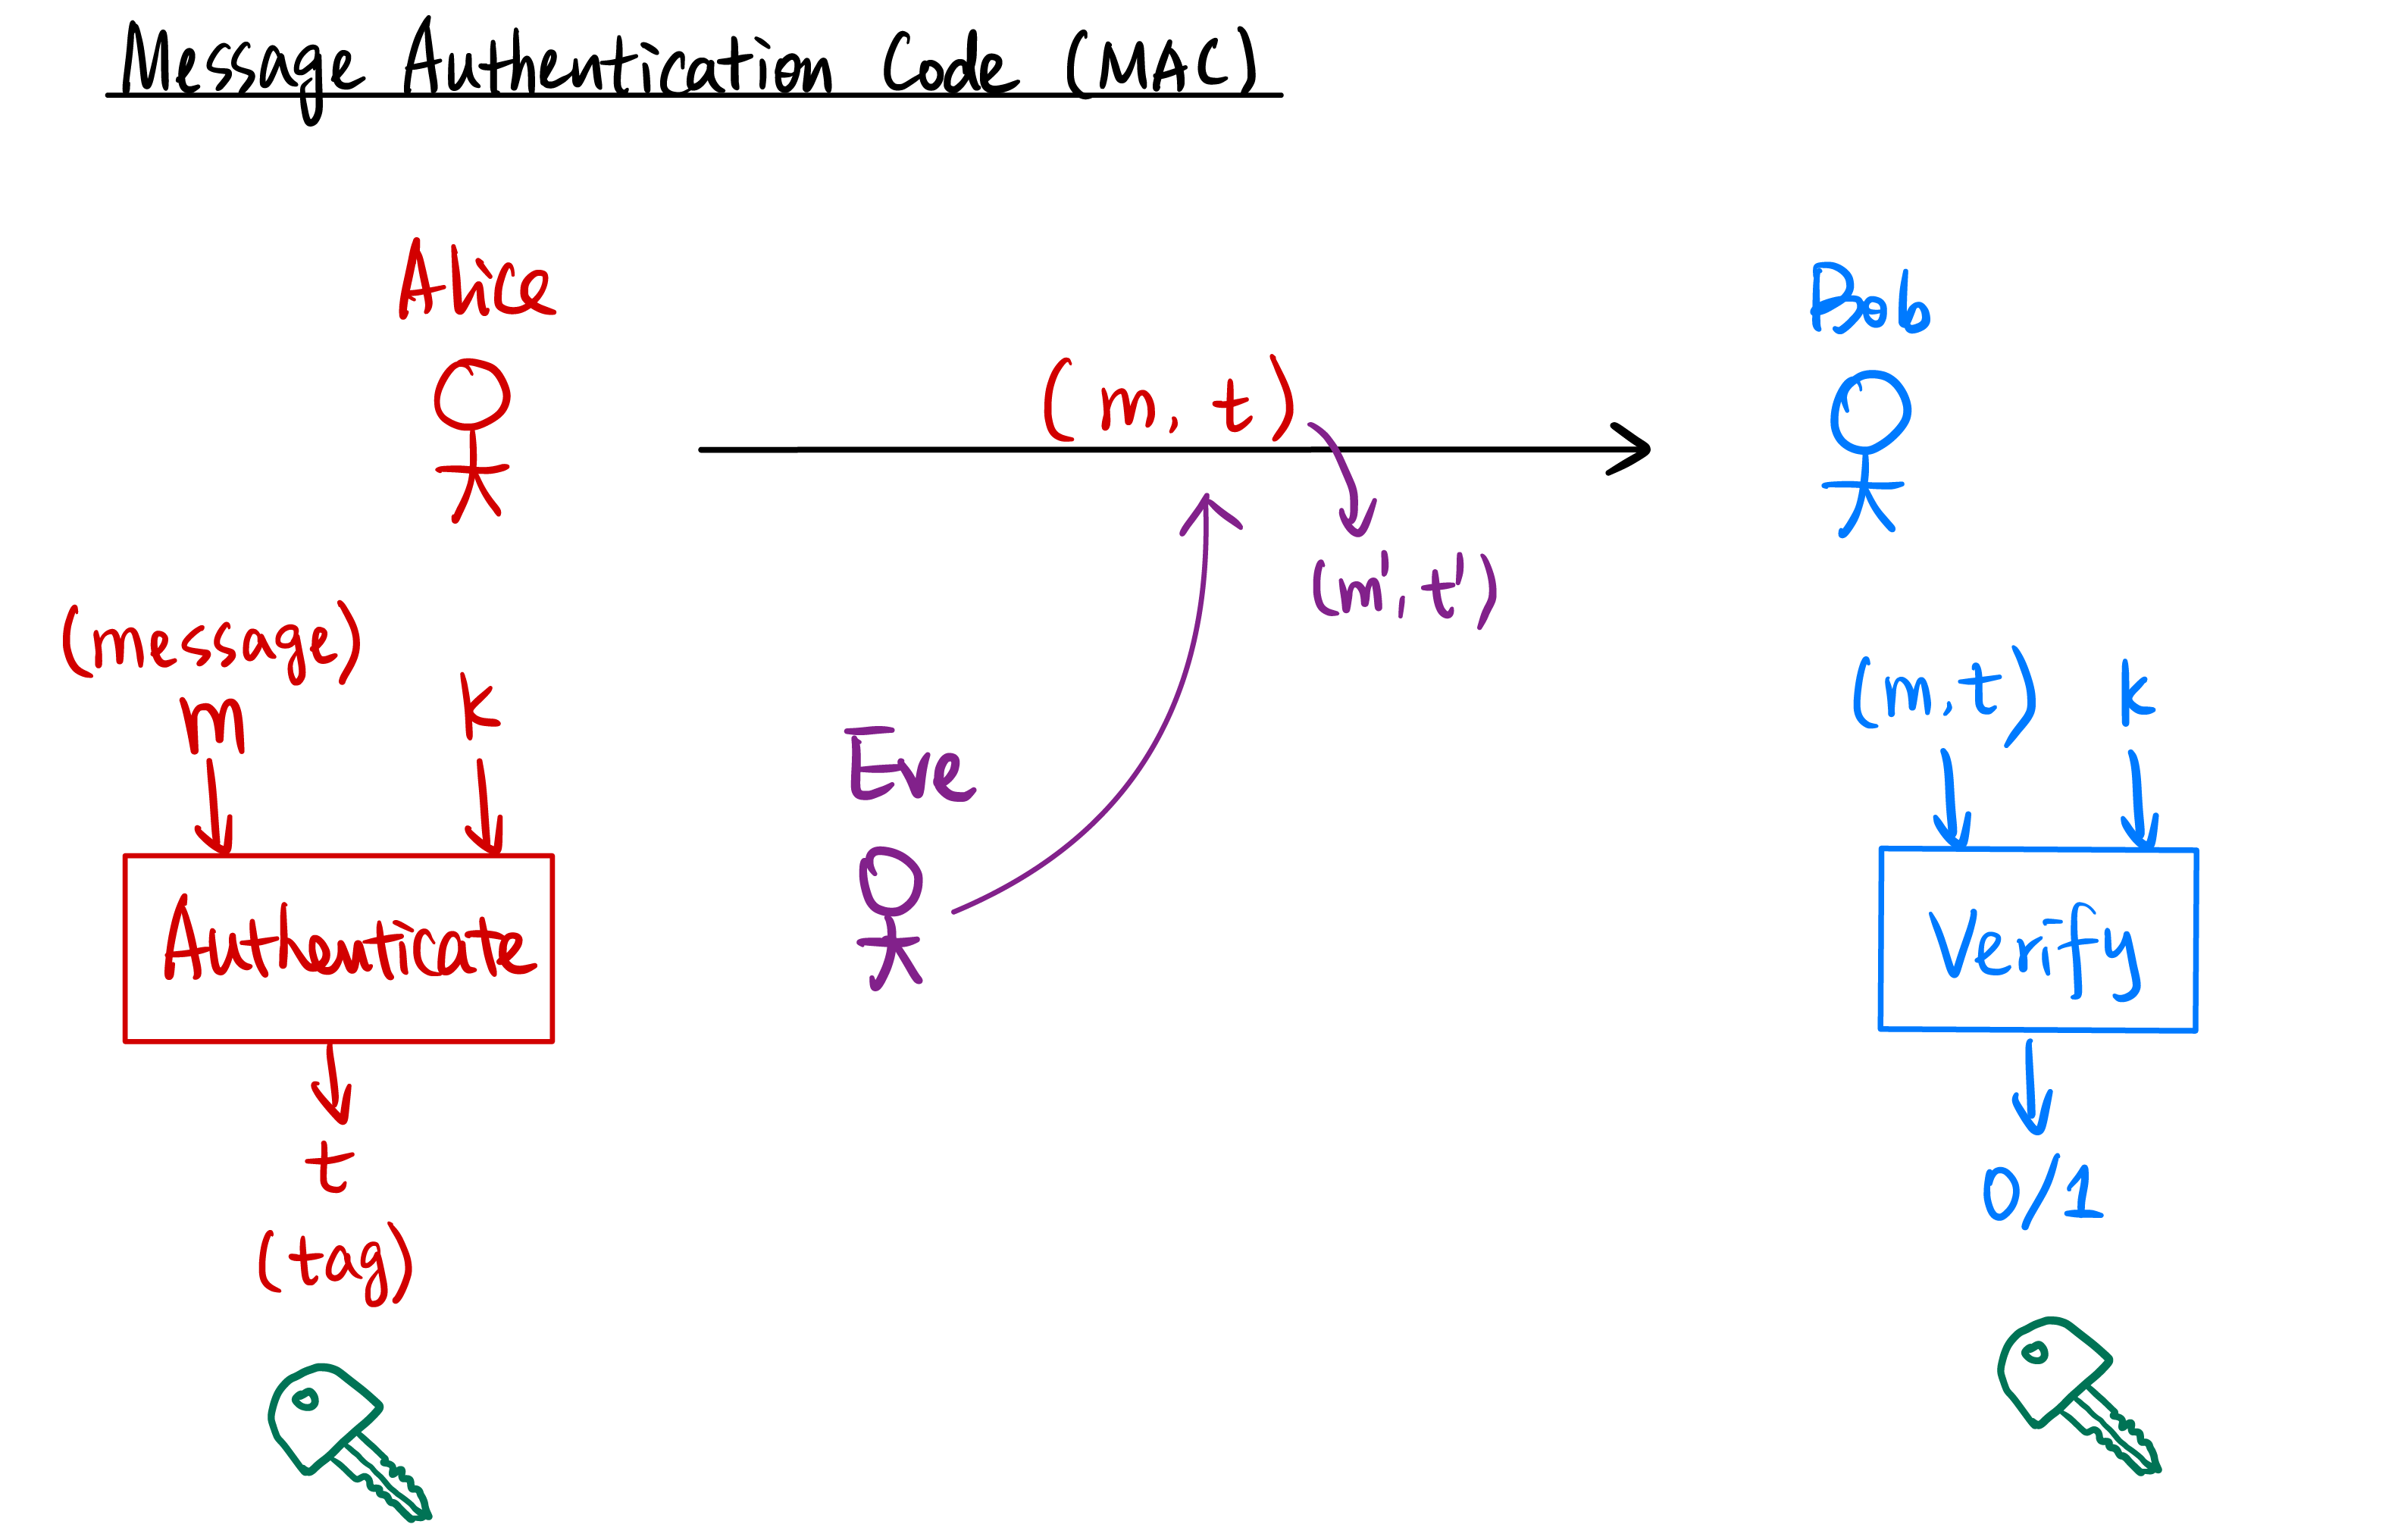
\includegraphics[width=0.8\textwidth]{images/2023-02-02/mac.png}
\end{center}

Using a public key $vk$ (verification key) and private key $sk$ (secret/signing key), Alice can sign a message $m$ using signing key $sk$ to get a \emph{signature} $\sigma$. Bob verifies $(m, \sigma)$ is valid using $vk$. This is called a Digital Signature.

\begin{center}
    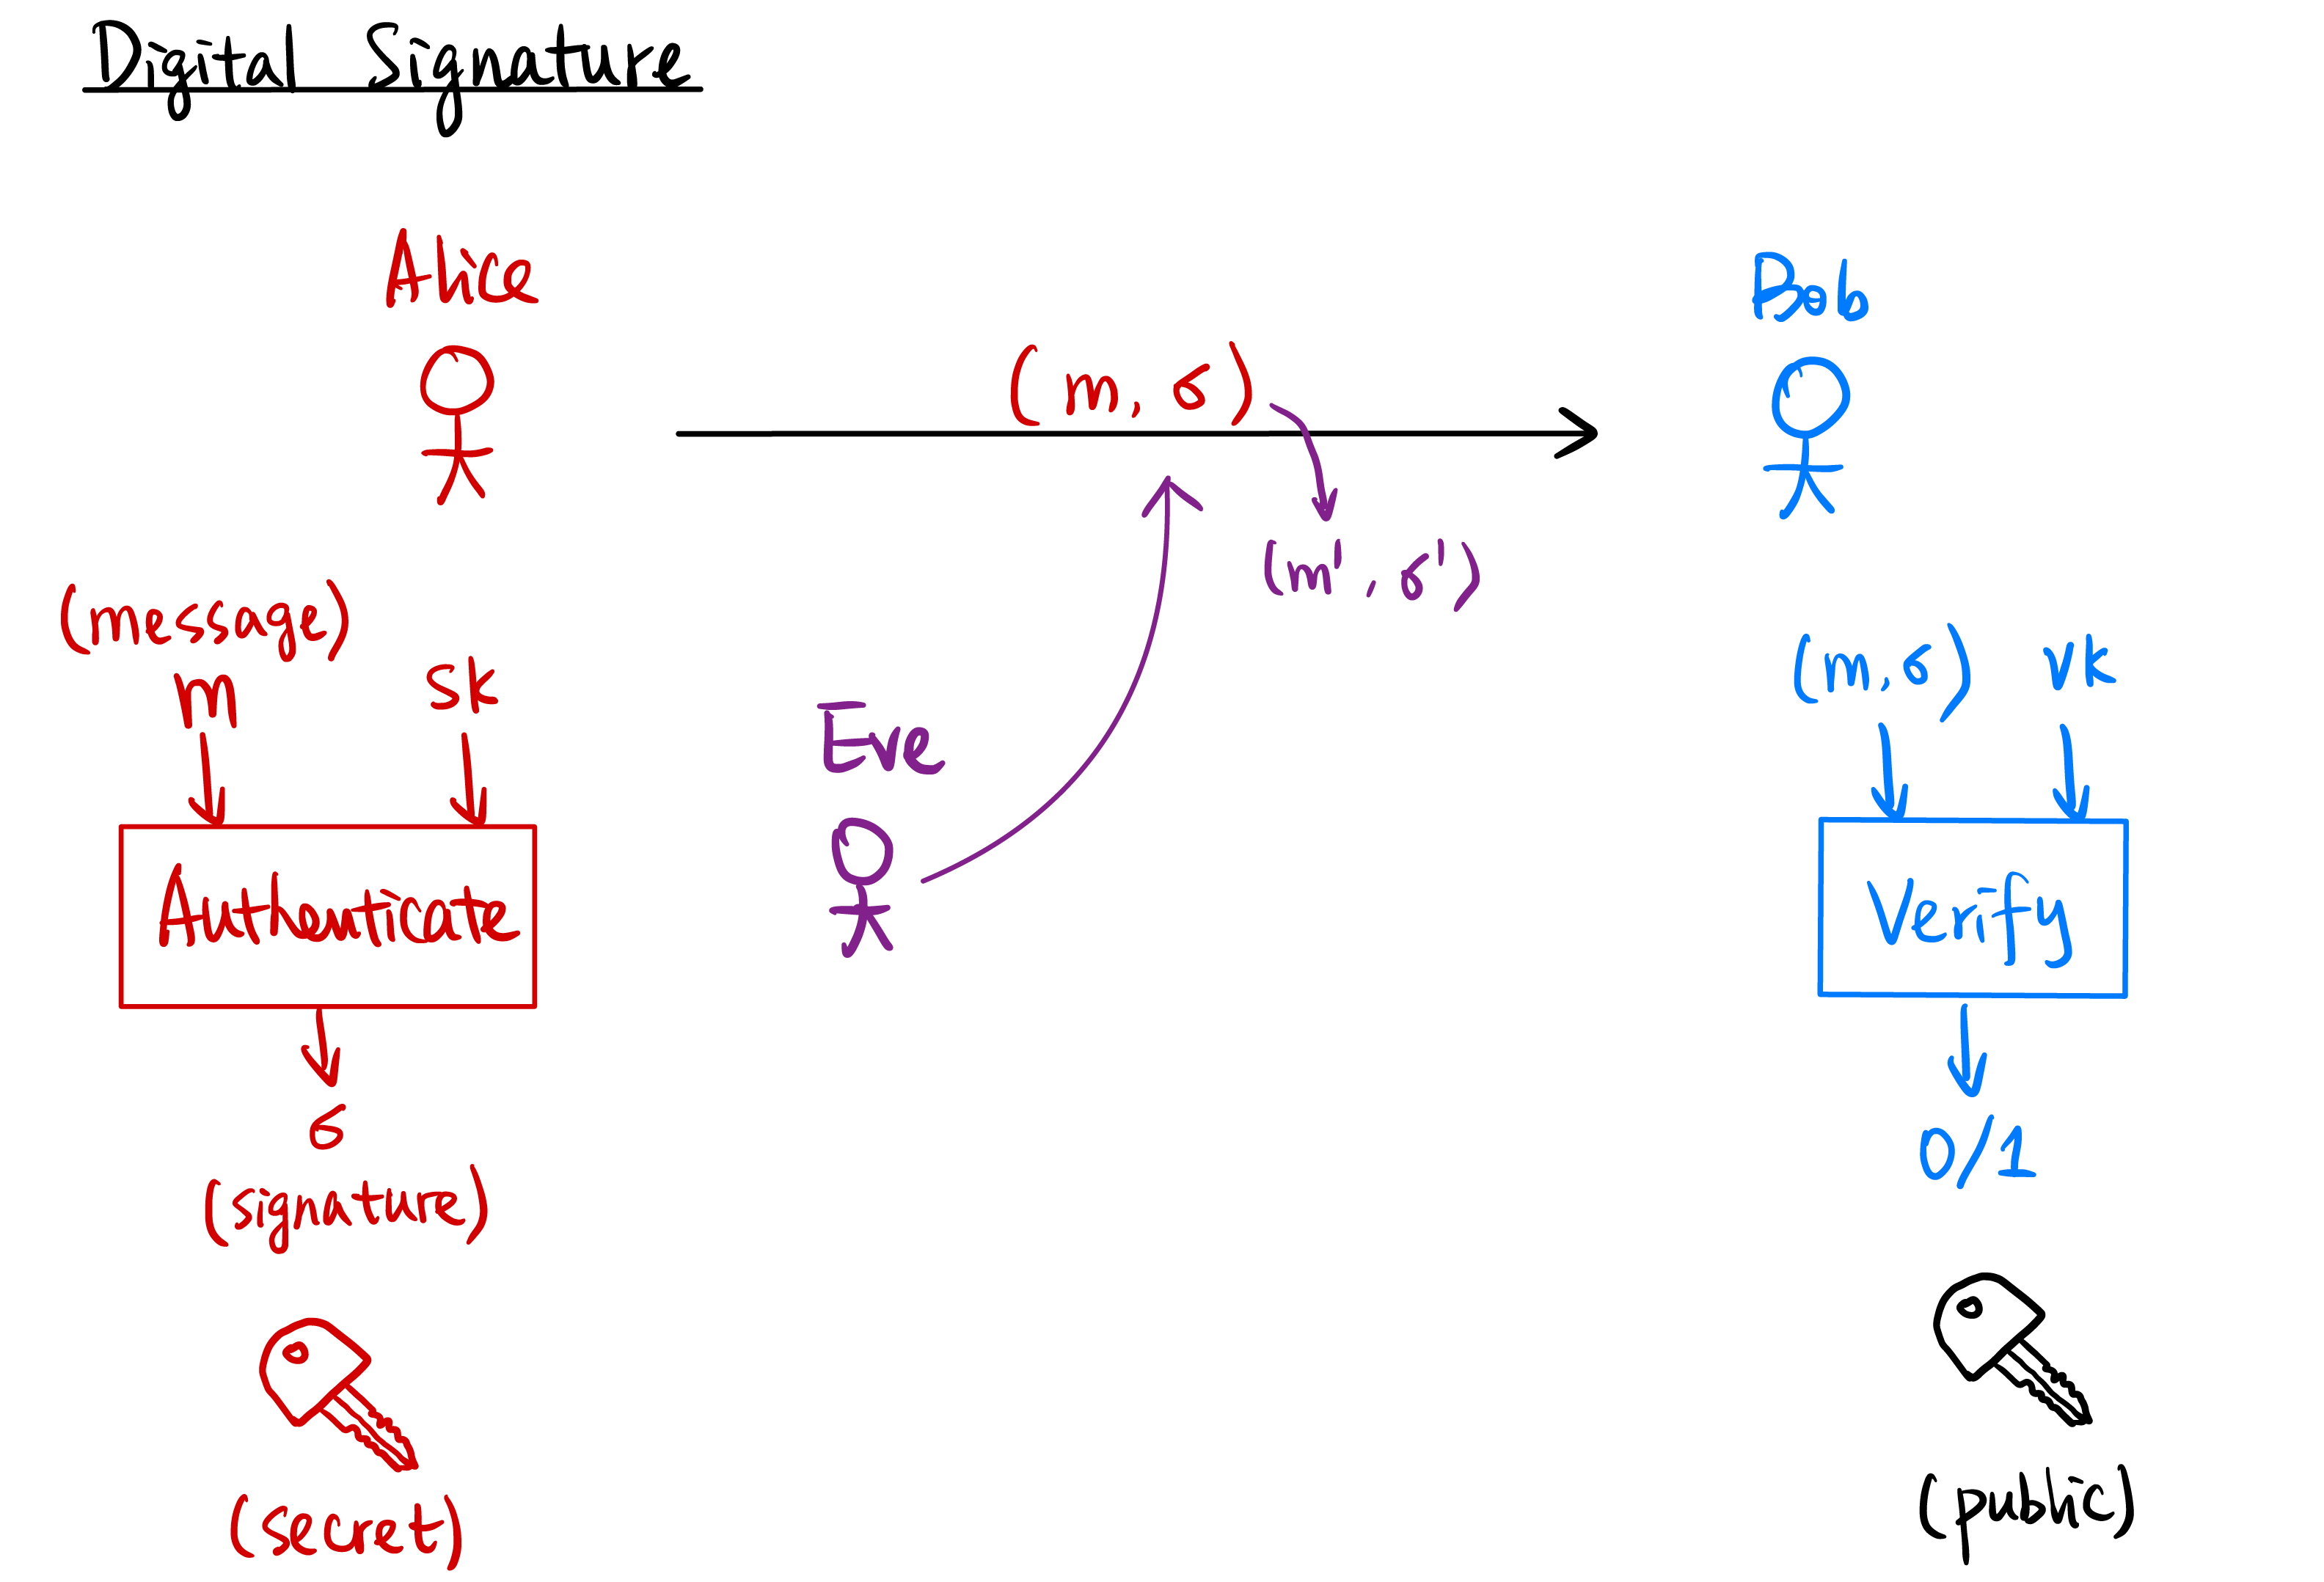
\includegraphics[width=0.8\textwidth]{images/2023-02-02/signature.png}
\end{center}

\subsubsection{Syntax}\label{sec:message-integrity:syntax}
The following is the syntax we use for MACs and digital signatures.

A message authentication code (MAC) scheme consists of $\Pi = (\Gen, \mathsf{Mac}, \mathsf{Verify})$.
\begin{description}
    \item[Generation.] $k\leftarrow \Gen(1^\lambda)$.
    \item[Authentication.] $t \leftarrow \mathsf{Mac}_k(m)$.
    \item[Verification] $0/1 := \mathsf{Verify}_k(m, t)$.
\end{description}

A digital signature scheme consists of $\Pi = (\Gen, \mathsf{Sign}, \mathsf{Verify})$.
\begin{description}
    \item[Generation.] $(sk, vk)\leftarrow \Gen(1^\lambda)$.
    \item[Authentication.] $\sigma \leftarrow \mathsf{Sign}_{sk}(m)$.
    \item[Verification] $0/1 := \mathsf{Verify}_{vk}(m, \sigma)$.
\end{description}

\subsubsection{Chosen-Message Attack}
Similar to chosen-plaintext attack from encryption, we have chosen-message attack security. An adversary chooses a number of messages to generate signatures or tags for. After that, the adversary will try to generate another valid pair of message and tag. We want to make sure that generating a new pair of message and tag is hard.

\begin{center}
    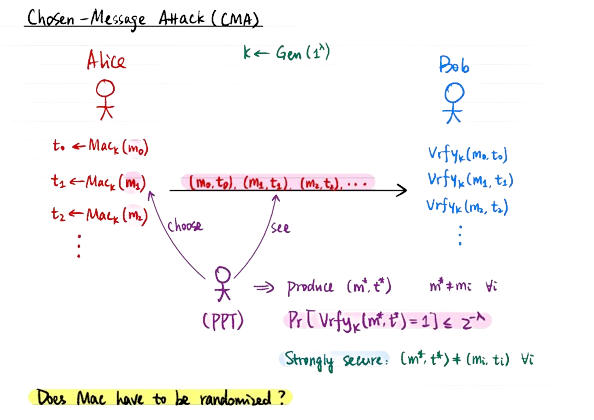
\includegraphics[width=0.8\textwidth]{images/2023-02-02/cma.png}
\end{center}

\subsubsection{Constructions}
Very briefly, we discuss constructions for MAC and digital signatures.

Using block ciphers, we have CBC-MAC. Using a hash function, we have HMAC.

For digital signatures, we have RSA which relies on the RSA assumption, or DSA which relies on discrete-log algorithms. There are also lattice signature schemes for post-quantum digital signatures.
%!TEX root = ../notes.tex
\section{February 5, 2024}
\label{20240205}

\subsection{Announcements}

\begin{itemize}
    \item New room! Due to more enrollment, starting next lecture we will be in Smith-Buonanno 106.
    \item Hiring more UTAs! If you know anyone who is qualified and interested, please let us know.
\end{itemize}

\subsection{Message Integrity}

Last lecture, we touched upon methods of authenticating a message. The symmetric-key version is called a MAC (message authentication code), the public-key version is called a digital signature. Let's review what we covered last time.

\subsubsection{Message Authentication Code}
To authenticate a message, Alice will use the private key $k$ to tag a message $m$ with a tag $t$. Bob will verify that $(m, t)$ is valid with key $k$.

\Graphic{images/2023-02-07/mac.png}{0.7}

\subsubsection{Digital Signature}
\label{sec:feb7-ds}
Similarly we have the public-key version. Alice has a secret key $sk$ to sign message $m$ with signature $\sigma$. Bob (or anyone) can verify with the public key $pk$ that $(m, \sigma)$ is a valid signature.

\Graphic{images/2023-02-07/ds.png}{0.7}

\subsubsection{Syntax}
Recall the syntax of MAC and digital signatures (see \cref{sec:message-integrity:syntax}).

A message authentication code (MAC) scheme consists of $\Pi = (\Gen, \mathsf{Mac}, \mathsf{Verify})$.
\begin{description}
    \item[Generation.] $k\leftarrow \Gen(1^\lambda)$.
    \item[Authentication.] $t \leftarrow \mathsf{Mac}_k(m)$.
    \item[Verification] $0/1 := \mathsf{Verify}_k(m, t)$.
\end{description}

A digital signature scheme consists of $\Pi = (\Gen, \mathsf{Sign}, \mathsf{Verify})$.
\begin{description}
    \item[Generation.] $(sk, vk)\leftarrow \Gen(1^\lambda)$.
    \item[Authentication.] $\sigma \leftarrow \mathsf{Sign}_{sk}(m)$.
    \item[Verification] $0/1 := \mathsf{Verify}_{vk}(m, \sigma)$.
\end{description}

\subsubsection{Chosen-Message Attack}
Similar to chosen-plaintext attack from encryption, we have chosen-message attack security. An adversary chooses a number of messages to generate signatures or tags for. After that, the adversary will try to generate another valid pair of message and tag. We want to make sure that generating a new pair of message and tag is hard.

\begin{center}
    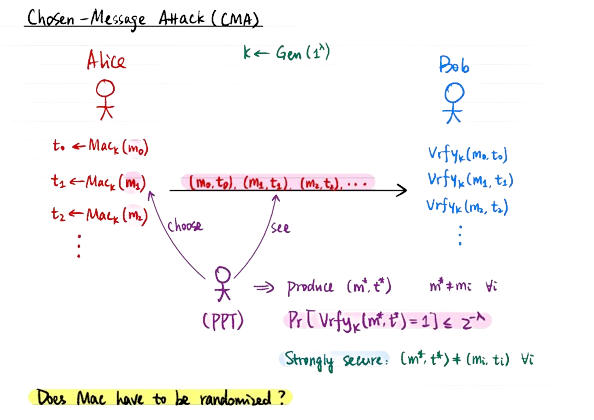
\includegraphics[width=0.8\textwidth]{images/2023-02-02/cma.png}
\end{center}

\begin{center}
    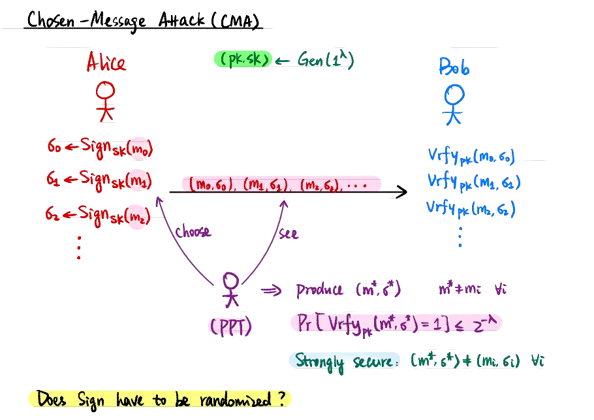
\includegraphics[width=0.8\textwidth]{images/2023-02-02/cma2.png}
\end{center}

\begin{ques*}
    Do the MAC and signature algorithms need to be randomized to be CMA secure?
\end{ques*}
No! Unlike CPA security, we don't need these algorithms to be randomized to be CMA secure.

% \subsubsection{Constructions}
% We can construct MAC pratically using
% \begin{itemize}
%     \item Block Cipher: CBC-MAC
%     \item Hash Functions: HMAC
% \end{itemize}

% We can construct digital signatures using
% \begin{itemize}
%     \item RSA signature: RSA Assumption.
%     \item DSA signature: Discrete Log Assumption
%     \item Lattice-Based Encryption Schemes (post-quantum secure).
% \end{itemize}

\subsection{RSA Signatures}
Our RSA signatures algorithm works very similarly to RSA encryption.

We generate two $n$-bit primes $p, q$. Compute $N:=p\cdot q$ and $\phi(N) = (p-1)(q-1)$. Again choose $e$ with $\gcd(e, \phi(N)) = 1$ and invert $d = e^{-1}\mod\phi(N)$. Given $N$ and a random $y\sampledfrom\ZZ_N^\times$, it's computationally hard to find $x$ such that $x^e\equiv y\mod N$.

Similarly, $sk := d$ and $vk := (N, e)$. To sign, we compute
\[\Sign_{sk}(m) := m^d\mod{N}.\]
To verify, we compute
\[\Verify_{vk}(m, \sigma):= \sigma^e\overset{?}{\equiv}m\mod N.\]

\begin{ques*}
    Are there any security issues with RSA as we have constructed it so far?
\end{ques*}

Thinking back to our definition of chosen-message attack, if Eve knows many messages and signatures, she can compute another pair of valid message and keys. If we have messages
\begin{align*}
    m_0, \sigma_0 & = m_0^d\mod N \\
    m_1, \sigma_1 & = m_0^d\mod N
\end{align*}
We can compute $m^* := m_0\cdot m_1$ and $\sigma^* := \sigma_0 \cdot \sigma_1 = (m_0\cdot m_1)^d\mod N$.

We can do linear combinations of messages, as well as raising messages to arbitrary exponents, and we can get other messages with valid signatures.

There is an easy solution, however. We can hash our message $m$ before we sign, like so
\begin{align*}
    \Sign_{sk}(m)           & := {\color{red}H(}m{\color{red})}^d\mod{N}                         \\
    \Verify_{vk}(m, \sigma) & := \sigma^e\overset{?}{\equiv}{\color{red}H(}m{\color{red})}\mod N
\end{align*}
where $H$ is a hash function\footnote{A hash function is, briefly, a function that produces some random output that is hard to compute the inverse of.}. This is a commonly known technique called `hash-and-sign'.

\subsubsection{Other Signature Schemes}

There are also other signature schemes that rely on other hardness assumptions.

\begin{itemize}
    \item RSA signatures rely on the RSA assumption.
    \item Schnorr/DSA signatures rely on the discrete log assumption.
    \item Lattice-based encryption schemes are post-quantum secure and rely on the hardness of certai lattice problems.
\end{itemize}

\subsection{A Summary So Far}
\label{sec:feb7-summary-so-far}
To summarize, here's all we've covered so far:
\begin{center}
    \begin{tabular}{@{}lll@{}}
        \toprule
                                      & \textbf{Symmetric-KePy}                                                                & \textbf{Public-Key}                                                                   \\ \midrule
        \textbf{Message Secrecy}      & \begin{tabular}[c]{@{}l@{}}Primitive: SKE\\ Construction: Block Cipher\end{tabular}    & \begin{tabular}[c]{@{}l@{}}Primitive: PKE\\ Constructions: RSA/ElGamal\end{tabular}   \\ \midrule
        \textbf{Message Integrity}    & \begin{tabular}[c]{@{}l@{}}Primitive: MAC\\ Constructions: CBC-MAC/HMAC\end{tabular}   & \begin{tabular}[c]{@{}l@{}}Primitive: Signature\\ Constructions: RSA/DSA\end{tabular} \\ \midrule
        \textbf{Secrecy \& Integrity} & \begin{tabular}[c]{@{}l@{}}Primitive: AE\\ Construction: Encrypt-then-MAC\end{tabular} &                                                                                       \\ \midrule
        \textbf{Key Exchange}         &                                                                                        & Construction: Diffie-Hellman                                                          \\ \midrule
        \textbf{Important Tool}                & \begin{tabular}[c]{@{}l@{}}Primitive: Hash function\\ Construction: SHA\end{tabular}   &                                                                                       \\ \bottomrule
    \end{tabular}
\end{center}

\subsection{Authenticated Encryption}
\label{sec:feb7-authenticated-encryption}
Generally, Alice and Bob will first perform a Diffie-Hellman key exchange, then use that shared key to conduct Symmetric-Key Encryption.

\Graphic{images/2023-02-07/practice.png}{0.6}

In reality, we want to achieve both message secrecy and integrity \emph{at the same time}. For this, we can introduce Authenticated Encryption.

Our security definition is that our adversary can see the encryptions of many messages $m_0, m_1, m_2$. We want \textbf{CCA security}: that an adversary given previous ciphertexts and their decryptions cannot distinguish between the encryptions of a fresh pair of messages $m_0$ and $m_1$. \emph{Additionally}, we want the property of \textbf{unforgeability}, that our adversary cannot generate a $c^*$ that is a valid encryption, such that $\Dec_{k}(c^*)\neq m_i$ for any $i$.

\Graphic{images/2023-02-07/ae.png}{0.8}

Now that we have two new primitives, we can construct Authenticated Encryption schemes.

\subsubsection{Encrypt-and-MAC?}
Given a CPA-secure SKE scheme $\Pi_1(\Gen_1, \Enc_1, \Dec_1)$ and a CMA-secure MAC scheme $\Pi_2 = (\Gen_2, \Mac_2, \Verify_2)$.

We construct an AE scheme $\Pi = (\Gen, \Enc, \Dec)$ by composing encryption and MAC. We encrypt the plaintext and also compute the MAC the \emph{plaintext}.

\Graphic{images/2023-02-07/encrypt-and-mac.png}{0.3}

\begin{description}
    \item[$\Gen(1^\lambda)$:] $k_1:=\Gen_1(1^\lambda)$, $k_2:=\Gen_2(1^\lambda)$, output $(k_1, k_2)$.

    \item[$\Enc(m)$:] To encrypt, we first encrypt ciphertext $c_1 := \Enc_1(k_1, m)$ and sign message (in plaintext) $t_2 := \Mac_2(k_2, m)$ and output $(c_1, t_2)$.

    \item[$\Dec(m)$:] We have ciphertext $c = (c_1, t_2)$. Our message is $m:=\Dec_1(k_1, c_1)$, and our verification bit $b := \Verify_1(k_2, (m, t_2))$. If $b = 1$, output $m$, otherwise we output $\bot$.
\end{description}

\begin{ques*}
    Is this scheme secure? Assuming the CPA-secure SKE scheme and CMA-secure MAC scheme, does this give us both CPA-security and unforgeability?
\end{ques*}

MAC gives you \emph{unforgeability}---it doesn't even try to hide the message at all. It's possible that the MAC scheme reveals the message in the clear. For example, we might have a MAC scheme that includes the message in the signature \emph{in the clear} (which is still secure)!

Since MAC doesn't try to hide the message. If our MAC reveals something about our message, our composed scheme $\Pi$ doesn't give us CPA-security. You might still be able to infer something about the message.

We try something else\dots

\subsubsection{Encrypt-then-MAC}
We encrypt first, then we MAC on the \emph{ciphertext}.

\Graphic{images/2023-02-07/encrypt-then-mac.png}{0.3}

\begin{description}
    \item[$\Gen(1^\lambda)$:] $k_1:=\Gen_1(1^\lambda)$, $k_2:=\Gen_2(1^\lambda)$, output $(k_1, k_2)$.

    \item[$\Enc(m)$:] To encrypt, we first encrypt ciphertext $c_1 := \Enc_1(k_1, m)$ and sign message (in ciphertext) $t_2 := \Mac_2(k_2, {\color{red} c_1})$ and output $(c_1, t_2)$.

    \item[$\Dec(m)$:] We have ciphertext $c = (c_1, t_2)$. Our message is $m:=\Dec_1(k_1, c_1)$, and our verification bit $b := \Verify_1(k_2, ({\color{red} c_1}, t_2))$. If $b = 1$, output $m$, otherwise we output $\bot$.
\end{description}

You can prove that Encrypt-then-MAC schemes are CPA-secure and unforgeable.

\subsubsection{MAC-then-Encrypt}
Similarly, we can also MAC first, encrypt the entire ciphertext and tag concatenated.

\Graphic{images/2023-02-07/mac-then-encrypt.png}{0.3}

\begin{description}
    \item[$\Gen(1^\lambda)$:] $k_1:=\Gen_1(1^\lambda)$, $k_2:=\Gen_2(1^\lambda)$, output $(k_1, k_2)$.

    \item[$\Enc(m)$:] To encrypt, we first encrypt ciphertext $c_1 := \Enc_1(k_1, m)$ and sign message (in plaintext) $t_2 := \Mac_2(k_2, {\color{red} m||t_2})$ and output $(c_1, t_2)$.

    \item[$\Dec(m)$:] We have ciphertext $c = (c_1, t_2)$. Our message is ${\color{red} m||t_2}:=\Dec_1(k_1, c_1)$, and our verification bit $b := \Verify_1(k_2, (m, t_2))$. If $b = 1$, output $m$, otherwise we output $\bot$.
\end{description}

\begin{ques*}
    Is this secure?
\end{ques*}

This doesn't satisfy a stronger security definition called Chosen Ciphertext Attack (CCA) security. We might be able to forge ciphertexts that decrypt to valid message and tags.

\subsubsection{Chosen Ciphertext Attack Security}
On top of CMA security, the adversary can now request Alice to decrypt ciphertexts $c_0, c_1, \dots$.

\Graphic{images/2023-02-07/cca.png}{0.7}

We can prove that MAC-then-Encrypt is not CCA secure.

The moral of this is that \textbf{you should always use Encrypt-then-MAC.}

\subsection{Hash Function}
A hash function is a public function
\[H: {0, 1}^*\to {0, 1}^n\]
where $n$ is order $\Theta(\lambda)$.

\Graphic{images/2023-02-07/hash.png}{0.5}

We want our hash function to be collision-resistant. That is, it's computationally hard to find $x, y\in\left\{ 0, 1 \right\}^*$ such that $x\neq y$ yet $H(x) = H(y)$ (which is called a collision).

How might one find a collision for function $H: \{ 0, 1 \}^*\to \{ 0, 1 \}^n$. We can try $H(x_1), H(x_2), \dots, H(x_q)$.

If $H(x_1)$ outputs a random value, ${0, 1}^n$, what is the probability of finding a collision?

If $q = 2^n + 1$, our probability is exactly $1$ (by pigeon-hole). If $q = 2$, our probability is $\frac{1}{2^\lambda}$ (we have to get it right on the first try). What $q$ do we need for a `reasonable' probability?

\begin{remark*}
    This is related to the birthday problem. If there are $q$ students in a class, assume each student's birthday is a random day $y_i\sampledfrom [365]$. What is the probability of a collision? $q = 366$ gives $1$, $q = 23$ gives around $50\%$, and $q = 70$ gives roughly $99.9\%$.

    We can apply this trick to our hash function. If $y_i\sampledfrom [N]$, then $q = N+1$ gives us $100\%$, but $q = \sqrt{N}$ gives $50\%$ probability.
\end{remark*}

Knowing this, we want $n = 2\lambda$ (output length of hash function). If $\lambda = 128$, we want $n$ to be around $256$.

\subsubsection{Random Oracle Model}
Another way to model a hash function is the \emph{Random Oracle Model}. We think of our hash function to be an oracle (in the sky) that can \emph{only} take input and a random output (and if you give it the same input twice, the same output).

\Graphic{images/2023-02-07/oracle.png}{0.5}

There are proofs that state that no hash functions can be a random oracle. There are schemes that can be secure in the random oracle model, but are not using hash functions\footnote{Some constructions don't rely on this model.}.

In reality, hash functions are \emph{about as good as}\footnote{But can never be\dots} random oracles. Thinking of our hash functions as random oracles gives us a good intuitive understanding of how hash functions can be used in our schemes.

In this model, the best thing that an attacker can do is to try inputs and query for outputs.

\subsubsection{Constructions for Hash Function}
\begin{description}
    \item[MDS.] Output length $128$-bit. Best known attack is in $2^{16}$. A collision was found in 2004.
\end{description}
And we also have Secure Hash Functions (SHA), founded by NIST.
\begin{description}
    \item[SHA-0.] Standardized in 1993. Output length is 160-bit. Best known attack is in $2^{39}$.
    \item[SHA-1.] Standardized in 1995. Output length is $160$-bit. Best known attack is in $2^{63}$, and a collision \emph{was} found in 2017.
    \item[SHA-2.] Standardized in 2001. Output length of 224, 256, 284, 512-bit. The most commonly used is SHA-256.
    \item[SHA-3.] There was a competition from 2007-2012 for new hash functions. SHA-3 was released in 2015, and has output length 224, 256, 2384, 512-bit. This is \emph{completely different} from SHA-2.
\end{description}

\begin{remark*}
    The folklore is that during a session at a cryptography conference, a mathematician, Xiaoyun Wang, presented slide-after-slide of attacks on MDS and SHA-0, astounding the audience.
\end{remark*}
%!TEX root = ../notes.tex
\section{February 07, 2023}
\label{20230207}
\subsection{Announcements}
\textbf{Capstone}: 1515 is right now in the google form. 

\textbf{Security Pathway}: 1515 is one of the course for security pathway even it is not listed in the CAB system.

\subsection{Cryptographic Hash Function, \emph{continued}}
Recall that we defined a hash function to be a public and deterministic function for which it is computationally hard to find a collision. That is, finding two distinct strings $x, y$ such that $H(x) = H(y)$ is computationally difficult.

For the hash function, the input domain is arbitrary-length string, and the output is a fixed-length string - 256 bits. The security guarantee is Collision-Resistant Hash Function(CRHF).
\Graphic{images/2023-02-09/hash.png}{0.4}

One model that we sometimes use to facilitate our analysis is the random oracle model. We assume our hash function is a random oracle `in the sky', and the only thing you can to is to send a query to it. The oracle will produces random hashes and send it back to the queries.

This is a very strong assumption, thus it's difficult to achieve the model theoretically. However, in reality it kind of makes sense. Since you can only query it, it's way more difficult to find the collision.

If you are given an arbitrary output, it's extremely hard to find its input. But it is not the case for CRHF, since CRHF only assumes you can not find a collision, thus this model is tronger than CRHF.

\Graphic{images/2023-02-09/hash-oracle.png}{0.4}

\subsubsection{Constructions}
Apart from MD5, we had Secure Hash Functions(SHA), including SHA-0, SHA-1, SHA-2 and SHA-3.

The hash function constructions that are still in practice (and unbroken) are SHA-2 and SHA-3. 

\subsubsection{Applications}

\begin{description}
    \item[HMAC.] We can use a hash function to conduct a MAC. Computing a tag involves computing the hash function on the key appended to the message ($k||m$). It is computationally difficult to find another $k || m'$ that produces the same hash. This is a scheme that looks like
        \[\Mac_k(m) = H(k||m).\]

        However, an adversary could potentially attach some additional $s$ to $m$ to produce $m' = m||s$ such that they can easily compute $\mathsf{tag}' = H(\mathsf{tag}||s)$. This is due to the Merkle-Damgård construction of SHA-2, which associatively tags blocks of the message one-by-one.

        \Graphic{images/2023-02-09/md.png}{0.4}

        Therefore, in practice, we use a nested MAC like
        \[\Mac_k(m) = H(k||H(k||m))\]
        and just to be sure (that we're not reusing the key), we produce $k_1, k_2$ as such
        \[\mathsf{HMAC}_k(m) = H(k_1||H(k_2||m))\]
        such that $k_1 = k\oplus \mathsf{opad}$ and $k_2 = k\oplus\mathsf{ipad}$, some one-time pads.

    \item[Hash-and-Sign.] There are some other applications of a hash function. We've seen before with RSA that we want to Hash-and-Sign, removing any homomorphism that an adversary could exploit. Additionally, this allows us to sign larger messages since they are constant size after hashing.

    \item[Password Authentication.] Another application is password authentication. Instead of storing plaintext passwords on servers, websites can store a hash of the password instead. This means that the passwords are not compromised even if the server is compromised.

    \item[Deduplicate Files.] We can also use hash functions to deduplicate files. We can hash two files to produce identifiers $h_1$ and $h_2$. If $h_1\neq h_2$, this implies $D_1\neq D_2$. If $h_1 = h_2$, it almost always\footnote{If they are not equal, we've found a collision for our hash function, which is extremely unlikely.} implies that $D_1 = D_2$.

    \item[HKDF (Key Derivation Function).] We can derive more keys from a shared key, essentially using a hash function as a pseudorandom generator (PRG).

        For example, if there is $g^{ab}$ shared key, we can do
        \[\mathsf{HMAC}(g^{ab}, \textsf{salt})\]

        Using a random seed, and concatenating a public deterministic salt $G$, we can generate a random\footnote{Computationally random, because if our computational power were to be unbounded, we can try all strings.} string.

        \Graphic{images/2023-02-09/hkdf.png}{0.8}

    \item[Pseudorandom Generator (PRG).] Given a hash function $H$, we can generate a PRG easily for any length string by generating
        \begin{align*}
            \mathsf{seed}\sampledfrom \{0, 1\}^\lambda \longrightarrow & H(\mathsf{seed}||00\cdots 00) \\
                                                                       & H(\mathsf{seed}||00\cdots 01) \\
                                                                       & H(\mathsf{seed}||00\cdots 10) \\
                                                                       & \qquad\qquad \vdots
        \end{align*}

        We can take a bit of randomness (like the way we move our mouse, type keyboard, system properties) and generate our seed.

    \item[Fast Membership Proof (Merkle Tree).] Using hash functions, we can generate Merkle Trees to prove membership. In blockchains, this is equivalent to checking if a transaction occurred.

    \item[SKE Scheme?] Could we use this to encrypt? If we have a secret key $k\sampledfrom\{0, 1\}^\lambda$, can we just encrypt by
        \[\Enc_k(m) = H(k||m)\]
        Well, we can't decrypt for one without having unbounded computational power. If our plaintext $m$ comes from a small set, like $\{0, \dots, 10\}$, we could decrypt properly. However, this is not CPA-secure, since the adversary could just query for all the messages.

        \begin{remark}
            In general, all deterministic encryption schemes are not CPA-secure.
        \end{remark}
\end{description}

\subsection{Putting it Together: Secure Communication}
This is essentially what we want to do in the second project.

We use Diffie-Hellman Key Exchange between Alice and Bob to get shared $g^{ab}$. Hashing the shared key using an HKDF, we can get shared key $k = (k_1, k_2)$ (one for AES encryption, one for HMAC). Then, they perform authenticated encryption, namely Encrypt-then-MAC.

\begin{ques*}
    Are there any issues with this scheme?
\end{ques*}
An Eve could pretend to be Alice to Bob and Bob to Alice, fudging up their shared keys. This is called a \emph{Man-in-the-Middle} attack.

\subsubsection{Diffie-Hellman Ratchet}
What if a secret key gets leaked, or cracked? One simple way to fix this is to perform a Diffie-Hellman key exchange on every message. However, this incurs additionall communications costs.

Here's another idea: with every new message (when the direction of communications shifts), the party sending the message sends a new Diffie-Hellman public key for themselves. For example, if Bob is sending a message to Alice and he knows Alice's public key $g^{a_1}$ and his previous secret was $b_1$ (hence shared $g^{a_1b_1})$, Bob will generate new key $b_2, g^{b_2}$ and encrypt using $g^{a_1b_2}$, sending $g^{b_2}$ as public to Alice. Alice can recompute the shared key before decrypting.

\Graphic{images/2023-02-09/dh-ratchet.png}{0.7}

This is the protocol used in the Signal messaging app, and is what you will implement for Project 1.

\begin{ques*}
    What if $k_1$ is leaked?
\end{ques*}
We might have leaked one key, but the other keys are still computationally hard to compute. $k_1=g^{a_1b_1}$ is known, but it's equivalent to DDH to compute $g^{a_1b_2}$ or other keys.

\begin{ques*}
    What if $b_1$ is leaked?
\end{ques*}
We can compute key $k_1=g^{a_1b_1}$ and $k_2=g^{a_2b_1}$, but no further keys are leaked, and the next round of communications (after Bob refreshes his private key $b_2$) is still secure.

\subsection{Block Cipher}
To summarize, here's what we've seen so far (this table should be familiar):
\begin{center}
    \begin{tabular}{@{}lll@{}}
        \toprule
                                      & \textbf{Symmetric-Key}                                                                               & \textbf{Public-Key}                                                                   \\ \midrule
        \textbf{Message Secrecy}      & \begin{tabular}[c]{@{}l@{}}Primitive: SKE\\ Construction: \boxed{\textbf{Block Cipher}}\end{tabular} & \begin{tabular}[c]{@{}l@{}}Primitive: PKE\\ Constructions: RSA/ElGamal\end{tabular}   \\ \midrule
        \textbf{Message Integrity}    & \begin{tabular}[c]{@{}l@{}}Primitive: MAC\\ Constructions: CBC-MAC/HMAC\end{tabular}                 & \begin{tabular}[c]{@{}l@{}}Primitive: Signature\\ Constructions: RSA/DSA\end{tabular} \\ \midrule
        \textbf{Secrecy \& Integrity} & \begin{tabular}[c]{@{}l@{}}Primitive: AE\\ Construction: Encrypt-then-MAC\end{tabular}               &                                                                                       \\ \midrule
        \textbf{Key Exchange}         &                                                                                                      & Construction: Diffie-Hellman                                                          \\ \midrule
        \textbf{Important Tool}       & \begin{tabular}[c]{@{}l@{}}Primitive: Hash function\\ Construction: SHA\end{tabular}                 &                                                                                       \\ \bottomrule
    \end{tabular}
\end{center}
The only thing we haven't seen thus far is a block cipher. We first start with the definitions.

We saw earlier that a Pseudorandom Generator (PRG) produces a string that looks random. We also have Pseudorandom Functions (PRF), which are `random-looking' functions.

\subsubsection{Pseudorandom Function (PRF)}

Our Pseudorandom Function $F$ is a keyed function\footnote{In deterministic polynomial-time.} $F : \{0, 1\}^\lambda\times \{0, 1\}^n\to\{0, 1\}^m$, $F$ will take key $k$ and input $x$ to produce output $y$, $F(k, x) = y$.

Without knowing our key $k$, $F_k$ is computationally indistinguishable from some random $f\sampledfrom\{F\mid F\{0, 1\}^n\to \{0, 1\}^m\}$.

\Graphic{images/2023-02-09/prf.png}{0.8}

We have $2^\lambda$ possible $F_k$'s, and we have $(2^m)^{2^n}$ possible functions $f$. A computationally unbounded adversary could try all possible functions and distinguish our function, since $F_k$ lives in a subset of the space of $f$. However, in reality, we can assume that $F_k$ is computationally indistinguishable from any generic function.

\subsubsection{Pseudorandom Permutation (PRP)}

A further assumption is that our function is a bijection. $F_k$ is a keyed function from $F_k : \{0, 1\}^n\to\{0, 1\}^n$. We still have $2^\lambda$ possible $F_k$'s since there are $2^\lambda$

\Graphic{images/2023-02-09/prp.png}{0.8}

\begin{ques*}
    Again, how many possible $f$'s are there?
\end{ques*}
Our first string has $2^n$ choices to map to, our second choice has $2^n - 1$, so there are
\[(2^n)(2^n-1)(2^n-2)\cdots 1 = 2^n!\]

Still, this is a much larger number than $2^\lambda$, so we still make a computational assumption that our keyed function $F_k$ is still computationally indistinguishable from a random function $f$.
%!TEX root = ../notes.tex
\section{February 12, 2023}
\label{20240212}

\subsubsection{Pseudorandom Function (PRF), \emph{continued}}

A block cipher, at a very high level, is a pseudo random function.

Recall last time that we talked about pseudorandom \emph{generators} (PRG), which takes a seed and expands it into a long string of pseudorandom bits. This ``random-looking'' \textbf{string} is computationally indistinguishable from a truly random string.

A pseudorandom \emph{function} (PRF) is a ``random-looking'' \textbf{function} that takes a key and an input and produces an output. This function is computationally indistinguishable from a truly random function.

More formally, our pseudorandom function $F$ is a keyed function\footnote{In deterministic polynomial-time.} $F : \{0, 1\}^\lambda\times \{0, 1\}^n\to\{0, 1\}^m$, $F$ will take key $k$ and input $x$ to produce output $y$, $F(k, x) = y$.

Without knowing our key $k$, $F_k$ is computationally indistinguishable from some random $f\sampledfrom\{F\mid F\{0, 1\}^n\to \{0, 1\}^m\}$.

\Graphic{images/2023-02-09/prf.png}{0.8}

We have $2^\lambda$ possible $F_k$'s, and we have $(2^m)^{2^n}$ possible functions $f$. A computationally unbounded adversary could try all possible functions and distinguish our function, since $F_k$ lives in a subset of the space of $f$. However, in reality, we can assume that $F_k$ is computationally indistinguishable from any generic function.

\subsubsection{Pseudorandom Permutation (PRP)}

A further assumption is that our function is a bijection. $F_k$ is a keyed function from $F_k : \{0, 1\}^n\to\{0, 1\}^n$. We still have $2^\lambda$ possible $F_k$'s since there are $2^\lambda$

\Graphic{images/2023-02-09/prp.png}{0.8}

\begin{ques*}
    Again, how many possible $f$'s are there?
\end{ques*}
Our first string has $2^n$ choices to map to, our second choice has $2^n - 1$, so there are
\[(2^n)(2^n-1)(2^n-2)\cdots 1 = 2^n!\]

Still, this is a much larger number than $2^\lambda$, so we still make a computational assumption that our keyed function $F_k$ is still computationally indistinguishable from a random function $f$.

\subsection{Block Ciphers}
Looking back on \cref{sec:feb7-summary-so-far}, the last outstanding primitive was the block cipher. We saw this last lecture, we'll continue discussing the block cipher.

Recall that we had seen pseudorandom functions which are keyed functions that are computationally indistinguishable from \emph{all} random functions from $\{0, 1\}^n\to \{0, 1\}^m$. A stronger form of pseudorandom functions are pseudorandom permutations: a keyed bijective map between $\{0, 1\}^n\to \{0, 1\}^n$ that is computational indistinguishable from pseudorandom permutations.

Block ciphers are a special form of pseudorandom permutation. It is a keyed function
\[F : \{0, 1\}^\lambda\times \{0, 1\}^n\to \{0, 1\}^n\]
where $\lambda$ is the key length and $n$ is the block length. The practical construction of which is AES, which takes blocks of $n = 128$ and key length $\lambda = 128, 192, 256$ as choices.

\subsubsection{Modes of Operation}

\textbf{Electronic Code Book (ECB) Mode:} We will run our block cipher on each block of our message individually. However, this is not CPA secure, since encryptions are deterministic. We need to `seed' our encryption with some random value.

\textbf{Cipher Block Chaining (CBC) Mode:} Instead of running on our block cipher on each block individually, every block will get an additional \emph{initialization vector} IV, which is $\mathsf{XOR}$ed onto each message before running the block cipher.

\Graphic{images/2023-02-14/cbc.png}{0.5}

We waved our hand over the fact that this is CPA secure---but it relies on the initialization vector being random.

\emph{What if our IV is not randomly sampled?} Consider an IV that is \emph{different} but not randomly sampled. For example, the IV is $0\cdots 00$ for the first message, $0\cdots 01$ for the second message, and so on. Do we still have security?

Unfortunately not. Say $m_1$ is $\mathsf{XOR}$ed onto $0\cdots 01$, an adversary under CPA can choose plaintext that is $m_1$ with its last bit flipped, such that $v_1$ is manipulated and the block cipher is again deterministic.

It is crucial that IV is randomly selected, and that the next IVs for future blocks (of the same message) are also pseudorandom (that are the previous ciphertext, which is okay).

\textbf{Chained Cipher Block Chaining (Chained-CBC) Mode:} We touched on this earlier, but there is a mode of operation of CBC that feeds the last cipher block as the new IV for the next message.

\Graphic{images/2023-02-14/ccbc.png}{0.7}

Similar to the case earlier, an adversary here can select a next message \emph{based on} their knowledge of the previous ciphertext and hence the upcoming IV.

This makes chained-CBC \emph{very subtly} different than CBC. If we squint our eyes enough, it just looks like sending a single message using CBC mode. The key difference is that between rounds of communication $m$ and $m'$, an adversary could influence $m'$ given the knowledge of the previous round.

\begin{remark*}
    Another note that this is \emph{very subtle}! To the extent that when \emph{Signal} was being developed, the course staff initially wrote the solution using Chained-CBC mode. This highlights the difficulty in creating real-world cryptographic systems!
\end{remark*}

\emph{The following will be new modes not covered last lecture:}

\textbf{Counter (CTR) Mode:} Instead of chaining each successive IV from the previous block ciphertexts, we'll encrypt \emph{only} the $\mathrm{IV}\sampledfrom \{0, 1\}^\lambda$, and $\mathsf{XOR}$ the encrypted $F_k(\mathrm{IV}+i)$ to mask $m_i$, like a one-time pad.

Another way to think about the CTR mode is that we're using $F_k$ and a random IV to generate a long enough one-time pad to pad the entire message.

\Graphic{images/2023-02-14/ctr.png}{0.5}

\emph{How do we decrypt?} Since we know the first IV, we can compute the one-time pads $F_k(\mathrm{IV} + i)$ and $\mathsf{XOR}$ with $m_i$s. This scheme is valid.

\emph{Is this CPA secure?} The $\mathsf{XOR}$ \emph{after} $F_k$ might throw you off and cast doubt in your mind. However, this mode of operation is (!) CPA-secure. Even if we know IV, $\mathrm{IV}+1, \mathrm{IV}+2, \cdots$, we can't figure out the output of $F_k$ that becomes our one-time pad (to do so constradicts the CPA security of our block cipher). The CPA security of each $F_k$ being pseudorandom guarantees the CPA security of this scheme.

\emph{What about a ``stateful CTR mode'' which just increments IV every successive time?} Instead of sending a new IV for the next message, we'll just increment the IV from before. Similar to Chained-CBC mode, the adversary will know the IV that is going into the next message. However, this doesn't \emph{really} help the adversary. They've never seen those encrypted IV values before, and hence cannot modify the message given this information.

This is a distinction from last time, where the IV was $\mathsf{XOR}$ed onto the message directly, which could be tampered with by an adversary who knows the IV.

\emph{What if IV is not randomly sampled?} Nothing really breaks down, unlike the previous case. We just want to make sure that two IVs are not reused and don't collide. If IVs collide, two blocks will have the same one-time pad, which is potentially a problem. This doesn't prevent us from using $0\cdots 00, 0\cdots 01, 0\cdots 10, \dots$ as our IV values at all. In practice, however, they are still randomly sampled to prevent collisions.

\emph{Can we parallelize this?} Yes, we can compute $F_k(\mathrm{IV} + i)$ in parallel and $\mathsf{XOR}$ onto each block. Similar for encryption and decryption.

\emph{Can we construct a PRG from a PRF?} Using a seed $(\mathrm{IV}, k)$, we can generate an $n\lambda$ bit string
\[G(k||\mathrm{IV}) = F_k(\mathrm{IV})||F_k(\mathrm{IV} + 1)||F_k(\mathrm{IV} + 2)||\cdots\]
In fact, we can get rid of IV entirely and start at $0$,
\[G(k) = F_k(0)||F_k(1)||F_k(2)||\cdots\]

Counter mode essentially uses this PRG with private $k$ to generate a long one-time pad which is used to pad the message. Another note is that in this mode, we don't even require a pseudorandom permutation, since we don't need to invert the function at any point.

\textbf{Output Feedback (OFB) Mode:} This is a mix of CBC and CTR modes. Successive one-time pad blocks are fed into the next $F_k$ as IV, and they are $\mathrm{XOR}$ed with the message after encryption.

\Graphic{images/2023-02-14/ofb.png}{0.7}

We have the same questions. \emph{How do we decrypt? Is this CPA secure? Is a ``stateful'' version of OFB secure? Can we use this to construct a PRG?}

We can decrypt similarly: we decrypt the first block, get the IV for the next block and continue on. All security is guaranteed by the same reasoning as in counter mode: we know IV but still cannot compute $F_k(\mathrm{IV})$. Similar to counter mode, this is another form of PRG (which chains successive blocks instead of using IVs in series) that generates a long one-time pad. Again, our IV doesn't need to be randomly sampled, but it should not collide with previous IV values.

A difference to counter mode is that we cannot parallelize this scheme. However, in both CTR and OFB modes, we can precompute the entire one-time pad in both encryption and decryption to happen in the offline phase. The online phase (when parties are communicating) is limited to cheap $\mathsf{XOR}$ operations.

\begin{ques*}
    We've listed \emph{a lot} of benefits to counter mode or output feedback mode. Why do people use CBC mode at all?
\end{ques*}
We've seen how things can go wrong catastrophically\footnote{We nearly made mistakes in this course!}. This is more true for counter mode than CBC mode. If our IV is reused in counter mode, our entire one-time pad has been exposed previously\footnote{$\mathsf{XOR}$ing our ciphertexts will give $m \mathsf{XOR} m'$.}. However, if our IV is reused in CBC mode, the worst that could happen is something akin to ECB mode, and no messages are compromised.

At the end of the day, \emph{engineers are quite oblivious to cryptographic schemes}! Libraries only specify for \emph{some key} and \emph{some IV}, so it is exceedingly easy to screw up your cryptograhic scheme by reusing IVs, etc. CBC mode is simply more foolproof and incurs better outcomes in case it is used incorrectly\footnote{However, if Peihan were to implement a block cipher scheme herself, would opt for counter mode.}.

\subsubsection{CBC-MAC}
We can use block ciphers to construct a MAC scheme. Splitting up our message into blocks, we feed blocks into $F_k$ and chain to next blocks. In the end, the final cipher output is our tag.

\Graphic{images/2023-02-14/cbc-mac.png}{0.5}

\emph{How do we verify?} We can just $\Mac$ the message again and check that the tag matches. If $F_k$ is invertible, we can also go the other way.

\emph{Is this CMA secure?}
\begin{itemize}
    \item
          Fixed-length messages of length $l\cdot n$? Yes, since we can only query for fixed-length messages, this gives us no additional information.
    \item
          Arbitrary-length messages? This is where problems arise---the adversary could first query for a message of 1 block, then 2 blocks, then 3 blocks, etc. By combining this information, they could produce new valid signatures.

          A concrete attack is an adversary querying for $\Mac(m)$ to produce $\mathsf{tag}$, then querying for $\Mac(\mathsf{tag}) = \Mac(m||0) = \mathsf{tag}'$ which allows the adversary to forge a new message.
\end{itemize}

\begin{remark*}
    Our constructions of authenticated encryption calls for an encryption scheme and MAC scheme. It's crucial that the two schemes have \emph{different keys}. Using the same key $k$ for both encryption and MAC can cuase issues (information from one could reveal something about the other).
\end{remark*}

We have a fix for the CMA-vulnerability in arbitrary-length messages:

\subsubsection{Encrypt-last-block CBC-MAC (ECBC-MAC)}
The vulnerability earlier was due to our encryption being \emph{associative}, so to speak.

We can fix this is to use a different key for the last block:

\Graphic{images/2023-02-14/ecbc-mac.png}{0.5}

We could also attach length of messages to the first block, or other techniques.

The nuance in CBC-MAC means that realistically, we almost always use HMAC.

\ques{For CBC-MAC, if we randomly sample the IV and include it in the tag, will this be CMA secure?}

No! Consider if the adversary queries for the tag of $m := m_1 || m_2 || m_3$ and receive the tag $t := (\text{IV}, \text{tag})$.

The adversary can generate a new valid tag for $m^* := m_1 \oplus \text{IV} || m_2 || m_3$ and $t^* := (0^n, \text{tag})$.

\Graphic{images/2024/2024-02-12.png}{.8}

\subsection{Putting it Together}

Looking back at \cref{sec:feb7-summary-so-far}, we've collected everything we need so far for secure communication.

For Alice and Bob to communicate, they first exchange keys using a Diffie-Hellman key exchange, then perform authenticated encryption.

\Graphic{images/2023-02-14/communicate.png}{0.7}

However, this still does not mitigate against a man-in-the-middle attack. Thus, before exchanging keys, Alice and Bob should publish verification keys (to a digital signature scheme, see \cref{sec:feb7-ds}). Using this digital signature, Alice and Bob will each sign their Diffie-Hellman public values $g^a, g^b$ using their signing key, which will be attached to the message. They can respectively verify that these values came from each other, and not some Eve in the middle.
%!TEX root = ../notes.tex
\section{February 14, 2024}
\label{20240214}

\Graphic{images/2023-02-14/alice_and_bob.png}{0.8}
\begin{center}
    \href{https://xkcd.com/177/}{\emph{xkcd 177}}. \emph{Happy Valentine's Day! Stay safe by selecting authenticated encryption schemes (see \cref{sec:feb7-authenticated-encryption}) that are CPA secure and unforgeable to communicate with your date.}
\end{center}

This lecture we will go over the topics needed for the next project, Auth. Namely,
\begin{itemize}
    \item One-Sided Secure Authentication
    \item Password-Based Authentication
    \item Two-Factor Authentication (2FA)
    \item Putting it All Together: Secure Authentication
    \item Public Key Infrastructure (PKI)
\end{itemize}

Recall that we had a way for Alice and Bob to communicate securely, first exchanging a shared Diffie-Hellman key and then performing AES encryption.

\Graphic{images/2023-02-16/alice_and_bob.png}{0.8}

However, this is prone to a man-in-the-middle attack. One way to solve this is for parties to \emph{sign} their own Diffie-Hellman public values before sending, and then verify the other party's public value by using their public verification key.

\Graphic{images/2023-02-16/signed_alice_and_bob.png}{0.8}

\emph{Is this now secure against an adversary in the middle?} Yes, because the public values are guaranteed (via our digital signature scheme) by Alice and Bob's signing key. The man in the middle does not have access to the signing key, and cannot sign a phony public value.

However, how do we know the verification keys really belong to who we think they belong to? This is the problem of \emph{authentication}. We are sort of in a chicken and egg problem...

\subsection{One-Sided Secure Authentication}
In some circumstances, it's more difficult for a client to communicate their verification key to a server than it is for a server to do so. A server might publish their verification key, and trust that all clients are not compromised.

\Graphic{images/2023-02-16/one-sided_secure_authentication.png}{0.8}

\emph{What could an adversary potentially do?} The adversary could not pretend to be the server since they have no access to the server's signing key. The adversary \emph{can} pretend to be the client and talk to the server. The adversary could forward all messages sent to the server, and can also communicate $g^b, \sigma_b$ back to the client (it's a valid signature since it has not been modified).

At the end of this protocol, the client has Diffie-Hellman private $g^{ab}$ and the adversary and server will have $g^{eb}$ (where $g^e, e$ is a Diffie-Hellman keypair the adversary provided to the client). Whatever the client sends to the server cannot be decrypted by the adversary, since it is encrypted with $g^{ab}$, however, the server's communications \emph{could} be decrypted by the adversary.

This can be easily circumvented by requiring the server and user complete their handshake---the server could request a hash or encryption of the shared secret, and realize that they are communicating to an adversary when this cannot be forged by the man-in-the-middle.


\subsection{Password-Based Authentication}
Sometimes, you also want to \emph{authenticate} with a server using a password. The na\"ive implementation is that a user with an ID sends a hash of the password $h = H(\mathrm{password})$ to the server. The server stores $(\mathrm{ID}, h)$.

\Graphic{images/2023-02-16/password_authentication.png}{0.8}

In this case, an adversary could launch an \emph{Online Dictionary Attack} and try a lot of passwords with the server.

If the server were to be compromised, and its database compromised, the adversary can conduct an \emph{Offline Dictionary Attack} on the database. Additionally, the adversary can precompute all hashes and check against the database.

\emph{How can we prevent this? }

\subsubsection{Salting}

\Graphic{images/2023-02-16/salting.png}{0.8}

One way of ensuring that the hashing is non-deterministic is for servers to generate a $\mathrm{salt}\sampledfrom\{0, 1\}^s$ and send it to the user. The user will hash $H(\mathrm{password}||\mathrm{salt})$ and send that to the server. The server stores a database of $(\mathrm{ID}, \mathrm{salt}, \mathrm{h})$.

When logging in, the user first sends their ID to the server, the server will send the salt back, the user hashes their password, and the hash is sent to the server for verification.

\emph{Does this allow the user to use a weak password?} Nope! The adversary can always brute-force the password.

To further solve these problems, we can use \emph{peppering}. We send the salt to the user and the user computes hash $h = H(\mathrm{password}||\mathrm{salt})$. Then, we pick a random pepper and hash $h^* = H(h||\mathrm{pepper})$ and stores $h^*$. Now, even if the server is compromised, there is no way to find the preimage of $h^*$, so adversaries knowing $h^*$ will still have to do try all $2^p$ possible peppers for each dictionary guess. We still can't log into the server since the server hashes our login hash again.

Additionally, one strategy to make it \emph{even harder} for an adversary is to make hashing more difficult (time-consuming). For example, we can compose SHA256 in certain ways\footnote{The natural way is to hash multiple times, say 100. However, this is actually not more secure in the case of SHA256 but there are specific ways of composition. For example, there are application-specific integrated circuits (ASIC) that can compute hash functions very efficiently.}. There are also memory-hard hash functions, like scrypt.

\emph{Even with all this, is it still safe to use a weak password?} Nope! A dictionary attack is still possible, and with weak passwords will be hard to crack.

\subsubsection{Two-Factor Authentication}
Now we'll discuss how servers implement two-factor authentication.

For phone number verification, on signing up, the user sends a phone number with their password hash. The server stores their phone number. Every time, the server will generate challenge $r\sampledfrom\{0,1\}^k$

For app-generated codes, the user and server will first share a seed $\mathsf{seed}$ and use a pseudorandom function $F_\mathsf{seed}(\mathsf{time})$. The server and the user can input the same time, and the outputs will be the same. Generally, the server will test the last 30/60 seconds of values.

\Graphic{images/2023-02-23/2fa.png}{0.8}

% \subsection{SSH}

% This is \emph{exactly} how the SSH algorithm works.

% \Graphic{images/2023-02-16/ssh_protocol.png}{0.8}

% Let's work through the steps of GitHub's SSH setup to see how it works.

% \Graphic{images/2023-02-16/ssh_instruction.png}{0.8}

% The instructions are given for the EDDSA-25519 algorithm, which relies on elliptic curves.

% \begin{enumerate}
%     \item We first generate a signing keypair $(vk_A, sk_A) \leftarrow \Gen(1^\lambda)$ via

%           \texttt{\$ ssh-keygen -t ed25519 -C "your\_email@example.com"}

%           $vk_A$ is the \texttt{id\_ed25519.pub} (the public key) $sk_A$ is \texttt{id\_ed25519} (the private key).
%     \item We upload our public key to our account on GitHub. This is equivalent of communicating our $vk_A$ to GitHub.
%     \item When we're connecting via SSH to GitHub for the first time, our terminal will prompt us that this is a new server with a new verification key.

%           \texttt{> The authenticity of host `github.com (IP ADDRESS)' can't be established. \\
%               > RSA key fingerprint is SHA256:nThbg6kXUpJWGl7E1IGOCspRomTxdCARLviKw6E5SY8. \\
%               > Are you sure you want to continue connecting (yes/no)?}

%           which we can verify against GitHub's known verification keys\footnote{The security of our web upload to GitHub, or GitHub's site which publishes the verification key, relies on the security of the website, likely through TLS. But you could also imagine exchanging keys in person, etc. }. This is the equivalent of receiving a $vk_B$ from GitHub.
% \end{enumerate}


% \subsection{Public Key Infrastructure}

% \emph{How can we know who has which public keys on the internet?} We can rely on a Public Key Infrastructure (PKI) to know each other's public keys.

% If Bob purports to be \texttt{bob.com} and wants to prove that $vk_B$ belongs to him, Bob will send a certificate signing request (CSR) to a Certificate Authority (CA)\footnote{\emph{The higher beings that be}...this is companies like \emph{DigiCert}, \emph{Let's Encrypt}, etc.}.

% The CA will sign the message $(\mathtt{bob.com}, vk_B)$ and send that signature $\sigma$ back to Bob. This verifies that the user of \texttt{bob.com} holds signing key $sk_B$ with public key $vk_B$.

% \Graphic{images/2023-02-16/pki_cert.png}{0.8}

% The standard of which is the X.509 certificate.

% For example, when we try to access \texttt{facebook.com}, we can check that the certificate is valid\footnote{In browsers, this is represented by the lock symbol---clicking on that will allow you to verify that certificate.}

% \Graphic{images/2023-02-16/fb_cert.png}{0.8}

% This pivots on the fact that \emph{everyone} must know $vk$ of the certificate authority. We shift our trust from individual sites and users to the certificate authorities. Most devices have the $vk$s of trusted authorities built in.

% \subsubsection{Certificate Chain}
% In reality, there are several certificate authorities, and they also form \emph{chains} of certificate authorities.

% \Graphic{images/2023-02-16/cert_chain.png}{0.8}

% A Root CA\footnote{We mentioned earlier that CAs are built into devices. For example, \href{https://support.apple.com/en-us/HT213464}{here} is a list of all root certificates that are built-in for Apple devices. This can go wrong too! \href{https://en.wikipedia.org/wiki/Root_certificate\#Incidents_of_root_certificate_misuse}{CAs have been misused} which causes implications on the security of the internet.} with a known $(vk, sk)\Gen(1^\lambda)$ can first sign the $vk_1$ of an Intermediate CA1, producing cert $\mathsf{cert}_1 = \sigma \leftarrow \Sign_{sk}(vk_1)$.

% Then, the Intermediate CA1 can sign a certificate for Intermediate CA2, but we'll have to preserve this chain. Intermediate CA1 could produce cert $\sigma_1\leftarrow\Sign_{sk_1}(vk_2)$, but how do we know that $sk_1$ is valid? So, we'll need to include $vk_1$ and $vk_1$'s signature signed by $sk$. That is,
% \begin{align*}
%     \mathsf{cert}_2 = & vk_1, \sigma \leftarrow \Sign_{sk}(vk_1),   \\
%                       & vk_2, \sigma_2\leftarrow \Sign_{sk_1}(vk_2)
% \end{align*}
% Finally, Intermediate CA2 can sign Bob's verification key using their chain. Bob's certificate will contain
% \begin{align*}
%     \mathsf{cert}_B = & vk_1, \sigma \leftarrow \Sign_{sk}(vk_1),   \\
%                       & vk_2, \sigma_2\leftarrow \Sign_{sk_1}(vk_2) \\
%                       & vk_B, \sigma_B\leftarrow \Sign_{sk_2}(vk_B)
% \end{align*}
% \emph{How can an Intermediate CA restrict Bob's use of these certificates? What if Bob will then go on and start signing his own certificates for people?} We can concatenate information in each certificate that restricts its use. It could specify whether it is being issued to an \emph{end user}, or even additional information like validity time.

% To protect against CAs that get compromised, certificates are short-lived and have set validity times. Additionally, certificate authorities can publish revocation lists that browsers check against when validating a certificate.

%!TEX root = ../notes.tex
\section{February 21, 2024}
\label{20240221}

\subsection{Announcements}

\begin{itemize}
    \item Thank you to everyone for your intro videos!
    \item Please get a Dean's Note or doctor's note if you need extensions.
\end{itemize}

\subsection{A Brief Recap: Secure Authentication}

We'll quickly review what we have covered so far.

Recall that we have introduced a third party, the server, who is trusted by all party's and assigns certificates.

\Graphic{images/2024/2024-02-21-auth.png}{0.8}

After party's have their certificates, they can run two-sided authenticated key-exchange.

\Graphic{images/2024/2024-02-21-2-sided-kex.png}{0.8}

\subsection{Public Key Infrastructure}

\emph{How can we know who has which public keys on the internet?} We can rely on a Public Key Infrastructure (PKI) to know each other's public keys.

If Bob purports to be \texttt{bob.com} and wants to prove that $vk_B$ belongs to him, Bob will send a certificate signing request (CSR) to a Certificate Authority (CA)\footnote{\emph{The higher beings that be}...this is companies like \emph{DigiCert}, \emph{Let's Encrypt}, etc.}.

The CA will sign the message $(\mathtt{bob.com}, vk_B)$ and send that signature $\sigma$ back to Bob. This verifies that the user of \texttt{bob.com} holds signing key $sk_B$ with public key $vk_B$.

\Graphic{images/2023-02-16/pki_cert.png}{0.8}

The standard of which is the X.509 certificate.

For example, when we try to access \texttt{facebook.com}, we can check that the certificate is valid\footnote{In browsers, this is represented by the lock symbol---clicking on that will allow you to verify that certificate.}

\Graphic{images/2023-02-16/fb_cert.png}{0.8}

This pivots on the fact that \emph{everyone} must know $vk$ of the certificate authority. We shift our trust from individual sites and users to the certificate authorities. Most devices have the $vk$s of trusted authorities built in.

\subsubsection{Certificate Chain}
In reality, there are several certificate authorities, and they also form \emph{chains} of certificate authorities.

\Graphic{images/2023-02-16/cert_chain.png}{0.8}

A Root CA\footnote{We mentioned earlier that CAs are built into devices. For example, \href{https://support.apple.com/en-us/HT213464}{here} is a list of all root certificates that are built-in for Apple devices. This can go wrong too! \href{https://en.wikipedia.org/wiki/Root_certificate\#Incidents_of_root_certificate_misuse}{CAs have been misused} which causes implications on the security of the internet.} with a known $(vk, sk)\Gen(1^\lambda)$ can first sign the $vk_1$ of an Intermediate CA1, producing cert $\mathsf{cert}_1 = \sigma \leftarrow \Sign_{sk}(vk_1)$.

Then, the Intermediate CA1 can sign a certificate for Intermediate CA2, but we'll have to preserve this chain. Intermediate CA1 could produce cert $\sigma_1\leftarrow\Sign_{sk_1}(vk_2)$, but how do we know that $sk_1$ is valid? So, we'll need to include $vk_1$ and $vk_1$'s signature signed by $sk$. That is,
\begin{align*}
    \mathsf{cert}_2 = & vk_1, \sigma \leftarrow \Sign_{sk}(vk_1),   \\
                      & vk_2, \sigma_2\leftarrow \Sign_{sk_1}(vk_2)
\end{align*}
Finally, Intermediate CA2 can sign Bob's verification key using their chain. Bob's certificate will contain
\begin{align*}
    \mathsf{cert}_B = & vk_1, \sigma \leftarrow \Sign_{sk}(vk_1),   \\
                      & vk_2, \sigma_2\leftarrow \Sign_{sk_1}(vk_2) \\
                      & vk_B, \sigma_B\leftarrow \Sign_{sk_2}(vk_B)
\end{align*}
\emph{How can an Intermediate CA restrict Bob's use of these certificates? What if Bob will then go on and start signing his own certificates for people?} We can concatenate information in each certificate that restricts its use. It could specify whether it is being issued to an \emph{end user}, or even additional information like validity time.

To protect against CAs that get compromised, certificates are short-lived and have set validity times. Additionally, certificate authorities can publish revocation lists that browsers check against when validating a certificate.

\subsection{Case Studies}

\subsubsection{SSH}

\Graphic{images/2023-02-16/ssh_protocol.png}{0.8}

Let's work through the steps of GitHub's SSH setup to see how it works.

\Graphic{images/2023-02-16/ssh_instruction.png}{0.8}

The instructions are given for the EDDSA-25519 algorithm, which relies on elliptic curves.

\begin{enumerate}
    \item We first generate a signing keypair $(vk_A, sk_A) \leftarrow \Gen(1^\lambda)$ via

          \texttt{\$ ssh-keygen -t ed25519 -C "your\_email@example.com"}

          $vk_A$ is the \texttt{id\_ed25519.pub} (the public key) $sk_A$ is \texttt{id\_ed25519} (the private key).
    \item We upload our public key to our account on GitHub. This is equivalent of communicating our $vk_A$ to GitHub.
    \item When we're connecting via SSH to GitHub for the first time, our terminal will prompt us that this is a new server with a new verification key.

          \texttt{> The authenticity of host `github.com (IP ADDRESS)' can't be established. \\
              > RSA key fingerprint is SHA256:nThbg6kXUpJWGl7E1IGOCspRomTxdCARLviKw6E5SY8. \\
              > Are you sure you want to continue connecting (yes/no)?}

          which we can verify against GitHub's known verification keys\footnote{The security of our web upload to GitHub, or GitHub's site which publishes the verification key, relies on the security of the website, likely through TLS. But you could also imagine exchanging keys in person, etc. }. This is the equivalent of receiving a $vk_B$ from GitHub.
\end{enumerate}

\subsubsection{Secure Messaging}\label{sec:feb23-secure-messaging}

One solution is to have Alice sends an encrypted message, with a noted recipient (under Alice/Server's keys) to the server, the server decrypts it in the clear, and encrypts the message (using Bob/Server's keys) to send to Bob.

\Graphic{images/2023-02-23/server_relay.png}{0.7}

However, the message is completely revealed to the server in plaintext. Optimally, we don't want to do this, but many services do nevertheless. Alice and Bob can do a secure key exchange \emph{through} the server to get shared $g^{ab}$, and encrypt messages between them.

Alice will first encrypt using their shared key, then using their shared secret with the server, encrypt that ciphertext. The server will decrypt the first layer, encrypt that with Bob's key, and send that to Bob.

We note that the server is still the perfect middleman, but our trust assumption is that the server is semi-honest---it will honestly follow the protocol but can try to glean any additional information from them.

\emph{Why might we still adopt the first approach, sending messages in plaintext?} Alice and Bob needs to know their private keys, and remain `online' all the time. If they switch a device, or lose their phone, messages will get lost. Sending messages in plaintext avoids this scenario.

\subsubsection{Group Chats}
\emph{What about group chats? How might we implement this.}

When we move to group chats, there are more things we need to consider. For example, do we want to reveal this message to the server? In this case, Alice can send the message in the clear to the server and it is forwarded. Additionally, we might ask whether we want to hide the group structure from the server.

\Graphic{images/2023-02-23/group_chats.png}{0.6}

The first scenario is the same---users can send the encrypted message to the server, the server reveals the message and reencrypts to the group members.

We might posit that Alice, Bob and Charlie share keys $g^a, g^b, g^c$, then they jointly have shared secret $g^{abc}$. This is called multi-party key exchange. However, this is in fact very difficult and relies on strong primitives.

Signal and WhatsApp use two different approaches (agree on the same key or pairwise keys), but they both have tradeoffs. We'll continue this next lecture.

In general, there are two paradigms for group messaging. Either everyone uses the \emph{same} key, or everyone has a different key. In WhatsApp, Alice would use a symmetric ratchet with key $A, gr$ (Alice's key and group key) to send the message to the server, and WhatsApp will forward the same encrypted message to Bob and Charlie. While the group structure is revealed to the server, but the message contents are unbeknownst to the server.

\Graphic{images/2023-02-28/whatsapp.png}{0.6}

In Signal, on the other hand, every pair of users has a differnt key. If Alice wants to send a message to Bob and Charlie, Alice will encrypt two messages, one with Alice/Bob's key and another with Alice/Charlie's key. The server will forward the encrypted messages to the users respectively. In Signal, a double ratchet encryption is preformed between every pair of parties. Another guarantee is that the group structure can be hidden against the server---Alice sending individual messages to Bob and Charlie is indistinguishable from their group texts.

\Graphic{images/2023-02-28/signal.png}{0.6}


\subsection{Single Sign-On (SSO) Authentication}
Often, we'll `log in with Google' or `log in with Apple'\footnote{Even Brown has Shibboleth!}. A user will authenticate themselves with the authentication server (Google, Apple, Shibboleth), and will be issued a `token' (usually a signature/MAC) for them to then authenticate themselves against the service provider.

Implementations include OAuth or OpenID, which is the format used by Google/Apple/Facebook, etc. Within enterprises, Kerberos credentials allow for SSO as well as things such as printing, connecting to servers, etc.

\Graphic{images/2023-02-28/sso.png}{0.7}

\subsection{Zero-Knowledge Proofs}
As mentioned in our course outline, a Zero-Knowledge Proof (ZKP) is a scheme that allows a prover to prove to a verifier some knowledge that they have, without revealing that knowledge.

\emph{What is a proof?} We consider what a `proof system' is. For example, we'll have a \emph{statement} and a \emph{proof} that is a purported proof of that statement. What guarantees do we want from this proof system? If the statement is true, we should be able to prove it; and if the statement is false, we shouldn't be able to prove this. These are our guarantees of \emph{completeness} and \emph{soundness}.
\begin{description}
    \item[Completeness.] If a statement is true, there exists a proof that proves it is true.
    \item[Soundness.] If a statement is false, any proof cannot prove it is true.
\end{description}

Before next lecture, consider what it means for a proof system to be ``zero-knowledge''.

%!TEX root = ../notes.tex
% Scribe: Sudatta Hor
\section{February 26, 2024}
\label{20240226}

\subsection{Zero-Knowledge Proofs}
Recall from last lecture that a Zero-Knowledge Proof (ZKP) is a scheme that allows a prover to prove to a verifier some knowledge that they have, without revealing that knowledge.

\emph{What is a proof?} We consider what a `proof system' is. For example, we'll have a \emph{statement} and a \emph{proof} that is a purported proof of that statement. What guarantees do we want from this proof system? If the statement is true, we should be able to prove it; and if the statement is false, we shouldn't be able to prove this. These are our guarantees of \emph{completeness} and \emph{soundness}.
\begin{description}
    \item[Completeness.] If a statement is true, there exists a proof that proves it is true.
    \item[Soundness.] If a statement is false, any proof cannot prove it is true.
\end{description}

We can think of NP languages from a proof system perspective.

\begin{example}[Graph 3-Coloring]
    Consider the \emph{Graph 3-coloring}.

    \Graphic{images/2023-02-28/3color.png}{0.3}

    We define our language
    \begin{align*}
        L   & = \{G: G\text{ has a 3-coloring}\} \\
        \intertext{and relation}
        R_L & = \{(G, \textrm{3Col})\}
    \end{align*}
    Our statement will be that $G$ has a 3-coloring. Our proof is providing such a coloring $(G, \mathrm{3Col})\in R_L$.

    This satisfies completeness and soundness. Every 3-colorable graph has a proof that is the 3-coloring itself, and if a graph doesn't have a 3-coloring, it will not have a proof.
\end{example}

We can think of NP languages as a proof system. A language $L$ is in $\mathsf{NP}$ if $\exists \text{poly-time} V$ (verifier) such that
\begin{description}
    \item[Completeness.] $\forall x\in L, \exists w$ (witness) such that $V(x, w) = 1$.
    \item[Soundness.] $\forall x\not\in L, \forall w^*, V(x, w^*) = 0$.
\end{description}
The prover will prove to the verifier that they have knowledge of witness $w$ without revealing the witness itself.

\begin{definition}[Zero-Knowledge Proof System]
    Let $(P, V)$ (for \emph{prover} and \emph{verifier}) be a pair of probabilistic poly-time (PPT) interactive machines. $(P, V)$ is a zero-knowledge proof system for a language $L$ with associated relation $R_L$ if
    \begin{description}
        \item[Completeness.] $\forall (x, w)\in R_L$, $\Pr[P(x, w) \leftrightarrow V(x) \text{ outputs }1] = 1$. That is, if there is a $x\in L$ with witness $w$, a prover will be able to prove to the verifier that they have knowledge of $w$.
        \item[Soundness.] $\forall x\not\in L$, $\forall P^*$, $\Pr[P^*(x) \leftrightarrow V(x)\text{ outputs }1]\simeq 0$. That is, for every $x$ not in the language, our prover $P^*$ will not be able to prove its validity to $V$, with negligible probability. If $P^*$ is PPT, we call the system a \emph{zero-knowledge argument}.
    \end{description}

\end{definition}

\subsubsection{Honest-Verifier Zero-Knowledge}
Honest-Verifier Zero-Knowledge (HVZK) can be thought of as security against a semi-honest verifier. In this scenario, the verifier will follows the protocol honestly.

\[\exists\PPT\ S\text{ s.t. }\forall(x, w)\in R_L, \mathrm{View}_V(P(x, w)\leftrightarrow V(x))\simeq S(x)\]

That is, that the transcript can be simulated by a simulator $S$ without interaction with the verifier, and without $w$.

\subsubsection{Zero-Knowledge (Malicious Verifier)}

Now assume that the verifier is malicious. In other words, the verifier can deviate from the protocol in attempt to extract more information than intended. Note that a malicious verifier $V^*$ is unable to learn anything about $w$.

We need an additional property that this is actually \emph{zero-knowledge}\framedfootnote{That is, the prover could just send the witness in the clear to the verifier, which satisfies completeness and soundness.}. We want to say that the verifier is unable to extract any additional information from the interaction between the verifier and prover. That is, even without the witness, a verifier might be able to `simulate' this transaction \emph{by themselves}!

    We'll say $\forall \mathrm{PPT}\ V^*, \exists \mathrm{PPT}\ S$ such that $\forall (x, w)\in R_L$,
    \[\mathrm{Output}_{V^*}[P(x, w)\leftrightarrow V^*(x)]\simeq S(x).\]
    That is to say, for everything in the language, the output transcript between the prover and verifier can be \emph{simulated} by the simulator without knowledge of the witness\framedfootnote{This is \emph{counterintuitive}, because if any PPT can simulate the proof by themselves, how do we know we're even talking to a prover that has a witness? This is subtle, but we give extra power to the simulator that they are allowed to \emph{rewind} the verifier to some previous step. If the transcript can be simulated, then surely no information is leaked from the protocol.}.
    \Graphic{images/2023-02-28/zkp_definition.png}{0.7}

\subsubsection{Proof Knowledge}

If the prover is able to prove, then they must know a witness $w$.

\[ \exists E \text{ s.t. } \forall p^*, \forall x, \Pr[E^{P^*(\cdot)}(x) \text{ outputs }w \text{ s.t. }(x, w) \in R_L] \cong \Pr[p^* \leftrightarrow V(x) \text{ outputs } 1]\]

\subsubsection{Zero-Knowledge Proof of Knowledge}

So we've built up our four properties:
\begin{itemize}
    \item Completeness: The prover can prove whenever $x\in R_L$.
    \item Soundness: For any $x$ not in $R_L$, the prover can only prove $x\in R_L$ with \emph{negligible} probability.
    \item Zero Knowledge: The verifier does not gain any additional information from the proof. That is, a simulator could have `thought up' the entire transcript in their head given the ability to rewind.
    \item Proof of Knowledge: An even stronger guarantee than soundness (this implies soundness)---a prover must have the witness in hand to be able to prove $x\in R_L$. That is, an extractor could interact with the prover (and rewind) to be able to extract the information of $w$ from the interaction.
\end{itemize}

\subsection{Example: Schnorr's Identification Protocol}\label{sec:mar7-schnorr}
\begin{remark*}
    \emph{The following is a hodgepodge of (arguably) clearer notes taken for Peihan's previous cryptography seminar, as well as lecture and slides from the current offering of Applied Cryptography. The notation might not correspond to lecture 1-to-1, but they are the same protocols albeit with different symbols.}
\end{remark*}
Let $G$ be a cyclic group of prime order $q$ with generator $g$, $h = g^a$. We wish to prove the relation
\[R_L = \{(g^\alpha, \alpha)\}_{\alpha\in \ZZ_q}\]

The language $L$ is given by
\[L = \{ h\in G: \exists a \in \mathbb{Z}_q \text{ s.t. }h = g^a\}\]

However, this is exactly the entire group, i.e. $L = G$. 

Generator $g$ is known, and the prover wishes to prove that they have the discrete log of $h$ ($\alpha$ where $g^\alpha\equiv h$).

\Graphic{images/2023-03-02/schnorr.png}{0.75}

Completeness here is clear, the prover is able to produce such $s$ if the prover has knowledge of $\alpha$.

\subsubsection{Proof of Knowledge}

We wish that
\[\exists\PPT\ E\text{ s.t. }\forall\PPT\ P^*, \forall x\in L, E^{P^*(\cdot)}(x)\text{ outputs }w\text{ s.t. }(x, w)\in R_L\]
``That there exists an extractor that by interacting to the prover $P^*$ that can extract $w$/$\alpha$''

In this case, $E$ can rewind the prover as well. We do so as follows:

We get the prover to commit to some $r$ and $A := g^r$, and pick $2$ $\sigma$'s (rewinding) such that we have
\begin{align*}
    g^s                                                         & = h^\sigma\cdot u               \\
    g^{s'}                                                      & = h^{\sigma'}\cdot u            \\
    \intertext{Given these two equations, we can}
    g^{s - s'}                                                  & = h^{\sigma-\sigma'}
    \intertext{Then we have}
    g^{(s - s')(\sigma-\sigma')^{-1}} = h\Longrightarrow \alpha & = (s - s')(\sigma-\sigma')^{-1}
\end{align*}

\Graphic{images/2023-03-02/schnorr_pok.png}{0.75}

\subsubsection{Honest-Verifier Zero-Knowledge}
Can we also construct Zero-Knowledge for this protocol?
\[\forall\PPT\ V^*, \exists\PPT\ S \text{ s.t. }\forall (x, w)\in R_L, \mathrm{Output}_{V^*}(P(x, w)\leftrightarrow V^*(x))\overset{C}{\simeq} S(x)\]

We first do this for Honest-Verifier Zero-Knowledge. This can be thought of as security against a semi-honest verifier.
\[\exists\PPT\ S\text{ s.t. }\forall(x, w)\in R_L, \mathrm{View}_V(P(x, w)\leftrightarrow V(x))\simeq S(x)\]
That is, that the transcript can be simulated by a simulator $S$ without interaction with the verifier, and without $w$.

\Graphic{images/2023-03-02/schnorr_hvzk.png}{0.75}

We construct a simulator that gives us specific values of $A, \sigma, s$ where we can satisfy the equation $g^s = h^\sigma\cdot A$. Once we have $s$ and $\sigma$, we can easily compute the $A$ desired.

We don't have to generate them in order. Fixing $s$ and sampling $\sigma\sampledfrom \ZZ_g$, we can compute $g^s\cdot h^{-\sigma} = A$.

\subsection{Example: Diffie-Hellman Tuple}

We want to prove that $h = g^a, u = g^b, v = g^{ab}$ is a Diffie-Hellman Tuple in a cyclic group $\GG$ of order $q$ and generator $g$.

Our witness is `private exponent' $b$. Our statement is that $\exists b\in \ZZ_q$ such that $u = g^b$ and $v = h^b$.

\Graphic{images/2023-02-28/dh_tuple_proof.png}{0.7}

The prover will randomly sample $r\sampledfrom \ZZ_q$ and send to the verifier $A:=g^r$ and $B:=h^r$. The verifier randomly samples \emph{challenge} $\sigma \sampledfrom \{0, 1\}$, and sends this challenge bit to the prover. The prover will respond with $s := \sigma\cdot b + r\pmod{q}$. If the challenge bit was $0$, $s = r$ and the verifier verifies $A = g^S$ and $B = h^S$. If the challenge bit was $1$, $s = b + r$ and the verifier verifies $u\cdot A = g^s$ and $v\cdot B = h^S$.

\textbf{Completeness:} If this statement is true, the prover will be able to convince the verifier since they have knowledge of $b$.

Next lecture, we will prove proof of knowledge and honest-verifier zero-knowledge.
%!TEX root = ../notes.tex
% Scribe: Sudatta Hor
\section{February 28, 2024}
\label{20240228}

Today, we continue our discussion on zero-knowledge proofs. First, we will briefly give an overview on our next project involving anonymous online voting. We will revisit the example on the Diffie-Hellman Tuple, then discuss Non-Interactive Zero-Knowledge proofs. We will show how to achieve this using Fiat-Shamir Heuristic, talk about Elgalmal encryption for homomorphism and threshold decryption, and revisit how these relate to anonymous online voting.

\subsection{Anonymous Online Voting}

Say we have $n$ voters with votes $v_1, \dots, v_n \in \{ 0, 1\}$. Each voter encrypts their vote $\text{Enc}(v_1), \dots, \text{Enc}(v_n)$. Our goal is to compute the sum of these votes without having to decrypt each vote individually. Somehow, we must find $\text{Enc}(\sum v_i)$ then decrypt to find $\sum v_i$.

In this scenario, zero-knowledge proofs can be used to ensure that each vote $v_1$ is 0 or 1 and to verify that the sum $\sum v_i$ was computed correctly.

\subsection{Zero-Knowledge Proof of Knowledge}

Recall the five properties.

\begin{itemize}
    \item Completeness: The prover can prove whenever $x\in R_L$.
    \item Soundness: For any $x$ not in $R_L$, the prover can only prove $x\in R_L$ with \emph{negligible} probability.
    \item Proof of Knowledge: If a prover $P^*$ can prove, then they must know $w$.
    \item Honest-Verifier Zero-Knowledge (HVZK). An honest verifier doesn't learn anything about $w$.
    \item Zero Knowledge: A malicious $V^*$ doesn't learn anything about $w$.
\end{itemize}

\subsubsection{Sigma Protocol}

Last time, we saw two concrete examples. They both follow a paradigm called \textit{sigma protocols}. This is a three-round protocol. In the first round, a prover sends a message called a \textit{commitment}. In the second round, the verifier sends to the prover a challenge $\sigma$. Then, the prover must send a valid response for the challenge.

\subsection{Example: Diffie Hellman Tuple}

We want to prove that $h = g^a, u = g^b, v = g^{ab}$ is a Diffie-Hellman Tuple in a cyclic group $\GG$ of order $q$ and generator $g$.

Our witness is `private exponent' $b$. Our statement is that $\exists b\in \ZZ_q$ such that $u = g^b$ and $v = h^b$.

\Graphic{images/2023-02-28/dh_tuple_proof.png}{0.7}

The prover will randomly sample $r\sampledfrom \ZZ_q$ and send to the verifier $A:=g^r$ and $B:=h^r$. The verifier randomly samples \emph{challenge} $\sigma \sampledfrom \{0, 1\}$, and sends this challenge bit to the prover. The prover will respond with $s := \sigma\cdot b + r\pmod{q}$. If the challenge bit was $0$, $s = r$ and the verifier verifies $A = g^S$ and $B = h^S$. If the challenge bit was $1$, $s = b + r$ and the verifier verifies $u\cdot A = g^s$ and $v\cdot B = h^S$.

\textbf{Completeness:} If this statement is true, the prover will be able to convince the verifier since they have knowledge of $b$.

\textbf{Soundness:} Show that if the prover does not have $b$, the probability that they send a valid $S = \sigma b + r \mod q$ is negligible. The prover can be malicious and does not have to follow the protocol. In the first round, they do not have to send $A = g^r, B = h^r$, but they can send $A = g^{r_1}, B= h^{r_2}$.

\textbf{Proof of Knowledge:} Formally, $\exists \mathrm{PPT}\ E$ (called \emph{extractor}) such that $\forall P^*$ (potentially dishonest prover), $\forall x$,
\[\Pr[E^{P^*(\cdot)}(x) \text{ outputs }w\text{ s.t. }(x, w)\in R_L] \simeq \Pr[P^*\leftrightarrow V(x)\text{ outputs }1].\]
This is to say, the probability that the extractor can extract a witness is computationally indistinguishable from the probability of the prover successfully proving $x\in R_L$.

An extractor, interacting with a prover (not necessarily honest), should be able to \emph{extract} the witness $w$ out of its communication with the prover, with the additional power that it can rewind the prover.

\Graphic{images/2023-03-02/dh_extractor.png}{0.75}

The extractor can first pick $\sigma = 0$, which gives them $s$ such that $A = g^s, B = h^s$. Then, the extractor rewinds the protocol and issues challenge $\sigma' = 1$, gaining $s'$ such that $u\cdot A = g^{s'}$ and $v\cdot B = h^{s'}$.

Then, $u = g^{s-s'}$ and $v = h^{s-s'}$, combining these they can extract valid $b = s-s'\pmod{q}$. If the prover can always convince the verifier, then the extractor will always be able to extract the witness $w$.

\textbf{Honest-Verifier Zero-Knowledge}

\[\exists\PPT\ S\text{ s.t. }\forall(x, w)\in R_L, \mathrm{View}_V(P(x, w)\leftrightarrow V(x))\simeq S(x)\]

We want to ensure that the verifier does not know anything about the witness. 

\subsubsection{Non-Interactive Zero-Knowledge (NIZK) Proofs}
\Graphic{images/2023-03-07/sigma.png}{0.75}
These all fall under a class called Sigma Protocols (they look like a capital $\Sigma$). A prover will first commit to some $A$, the verifier issues a challenge $\sigma$, then the prover will provide a proof corresponding to their $A$ and $\sigma$.

What if we wanted to condense it into a protocol that was \emph{non-interactive}, and only relies on the prover sending \emph{one} round of `proof' to the verifier.

\Graphic{images/2023-03-07/nizk.png}{0.75}

Completeness and soundness are the same. What about our previous definition of zero-knowledge? For all verifiers, will the simulator be able to simulate the one-way transcript? This is equivalent to the simulator being able to prove the statement itself\footnote{This is generally impossible! For example, a NIZK for the DH tuple that satisfies Zero-Knowledge breaks the Decisional Diffie-Hellman assumption.

    For the sake of contradiction, say we had such a simulator. To distinguish whether $(g^a, g^b, g^c)\overset{c}{\simeq}(g^a, g^b, g^{ab})$, we can feed this to the simulator to get a proof, and check with the verifier whether the proof is valid. The proof is valid if and only if it is a valid tuple. This contradicts DDH. Such a simulator had better not exist. }. Since there is only one round, the simulator `loses' its ability to rewind the prover and verifier. In the plain model, we cannot achieve a NIZK proof.

To make NIZK proofs possible, there are a few models available to us.

\begin{mdframed}[style=mdgreenbox]
    \begin{description}
        \item[Common Random String/Common Reference String (CRS):] There is a trusted third-party that both parties have access to, who generates a shared reference string.

            The power that we give to the simulator is that the simulator is allowed to generate this random/reference string together with the proof. This should be indistinguishable against the real-world.

            In reality, the CRS can be generated in a \emph{key ceremony} between parties such that no party can interfere with the generated key.

    \end{description}
    \Graphic{images/2023-03-07/crs.png}{0.75}
    \emph{There are some formal proof definitions of Zero-Knowledge, etc elided here but are in the post-notes. }
\end{mdframed}

\begin{mdframed}[style=mdgreenbox]
    \begin{description}
        \item[Random Oracle (RO) Model:] The prover and verifier have access to a hash function and it is a random oracle (behaves as if it is a random function).

            The additional power we give to the simulator is that they can control the behavior of the random oracle.
    \end{description}
    \Graphic{images/2023-03-07/rom.png}{0.75}
\end{mdframed}

\subsubsection{Fiat-Shamir Heuristic}\label{sec:mar7-fiat-shamir}
We can convert any Sigma protocol into a NIZK under the random oracle model. Recall that the only thing that could have gone wrong is that $\sigma\sampledfrom D$ was not computed randomly. Instead of using a challenge from the verifier, the challenge becomes $\sigma: H(x||m_1)$, a hash of the transcript so far. Since both the prover and verifier have access to the hash function, the prover can generate a challenge for themselves. After that, the prover can generate response.

A malicious verifier has no control over $\sigma$ now, so a malicious verifier cannot do anything more than seeing the proof. A malicious prover also cannot produce a valid $\sigma$ without committing to a $m_1$ first before receiving $\sigma$.

We can transform any public-coin\footnote{Every message sent from the verifier is randomly sampled from a distribution, as a challenge.} HVZK of arbitrary number of rounds into a NIZK using the Fiat-Shamir heuristic in the random oracle model.

Every public coin challenge will become the hash of the transcript so far from a random oracle. This condenses the entire proof into a single message that can be sent to the verifier (and that a verifier at a later point in time can also verify).

\begin{example}
    The Fiat-Shamir Heuristic can also transform Schnorr's Identification Protocol into Schnorr's Signature Scheme in the RO model.

    We have a cyclic group $\GG$ of order $g$, and generator $g$.

    Public verification key $vk = g^a$, secret signing key $sk = a$.

    We condense the Schnorr's Identification Protocol into a NIZK proof. To sign a message $m$, the random coin sample contains a hash of $m$ as well, \todo{Incomplete}
\end{example}

\subsection{Putting it Together: Anonymous Online Voting}
\subsubsection{Homomorphic Encryption}
Homomorphic encryption refers to encryption that allows for operations on the ciphertext corresponding to operations on the plaintext.

For example, an additively homomorphic scheme has the property that
\[\Enc(m_1) + \Enc(m_2) = \Enc(m_1 + m_2).\]
Similarly for multiplicatively homomorphic schemes,
\[\Enc(m_1) \cdot \Enc(m_2) = \Enc(m_1 \cdot m_2).\]

\begin{example}[ElGamal Homomorphism]
    Let's look at the ElGamal encryption scheme. We have a cyclic group $\GG$ with generator $g$, public key $pk$.
    \begin{align*}
        \Enc_{pk}(m_1) & =(g^{r_1}, pk^{r_1}\cdot m_1) \\
        \Enc_{pk}(m_2) & =(g^{r_2}, pk^{r_2}\cdot m_2)
    \end{align*}
    We note that this is multiplicatively homomorphic (element-wise):
    \[\Enc_{pk}(m_1)\cdot \Enc_{pk}(m_2) = (g^{r_1 + r_2}, pk^{r_1 + r_2}\cdot (m_1\cdot m_2)) = \Enc_{pk}(m_1\cdot m_2).\]
    This gives us multiplicative homomorphism, but we want additive homomorphism (we want votes to add, not multiply).

    We can consider exponential ElGamal, where the message is a power of $g$ (and exponents add).
    \begin{align*}
        \Enc_{pk}(m_1) & =(g^{r_1}, pk^{r_1}\cdot g^{m_1}) \\
        \Enc_{pk}(m_2) & =(g^{r_2}, pk^{r_2}\cdot g^{m_2})
    \end{align*}
    then
    \[\Enc(m_1)\cdot \Enc(m_2) = (g^{r_1 + r_2}, pk^{r_1 + r_2}\cdot g^{m_1\cdot m_2}) = \Enc(m_1 + m_2).\]
    but how do we recover the message? We can decrypt (normally) to get $g^{m_1 + m_2}$, but solving for $m_1 + m_2$ is \emph{hard}, since it is a discrete log.

    However, we're using this in the context of online voting. If $m\in \{0, \dots, n\}$ for $n$ the total number of voters (some polynomial range). This is fine for our uses!\framedfootnote{Normally, we talk about exponents from exponentially large sizes. Here, we can solve the discrete log since $n$ is quite small.}
\end{example}
%!TEX root = ../notes.tex
% Scribe: Sudatta Hor
\section{March 4, 2024}
\label{20240304}

\subsection{Anonymous Online Voting}

Recall anonymous online voting.

Say we have $n$ voters with votes $v_1, \dots, v_n \in \{ 0, 1\}$. Each voter encrypts their vote $\text{Enc}(v_1), \dots, \text{Enc}(v_n)$. Our goal is to compute the sum of these votes without having to decrypt each vote individually. Somehow, we must find $\text{Enc}(\sum v_i)$ then decrypt to find $\sum v_i$.

There are three questions.
\begin{enumerate}
    \item How do we compute $\text{Enc}(\sum v_i)$?
    \item How do we ensure each vote is 0 or 1?
    \item Who decrypts $\text{Enc}(\sum v_i)$?
\end{enumerate}

\subsection{Additively Homomorphic Encryption}

\begin{enumerate}
    \item Additively homomorphic encryption is taking two encryptions $\text{Enc}(m_1)$ and $\text{Enc}(m_2)$ and combine them to get $\text{Enc}(m_1 + m_2)$.
    \item Multiplicatively homomorphic encryption is taking two encryptions $\text{Enc}(m_1)$ and $\text{Enc}(m_2)$ and getting the product $\text{Enc}(m_1 \cdot m_2)$.
\end{enumerate}

\begin{example}[Elgalmal Encryption]
\textbf{Elgamal Encryption:} Cyclic group $G$ with generator $g$, and the public key is given by $\text{pk} = g^{\text{sk}}$. The encryption of message $m_1$ is given by $\text{Enc}_\text{pk}(m_1) = (g^{r_1}, \text{pk}^{r_2} \cdot m_1)$ and the encryption of message $m_2$ is given by $\text{Enc}_\text{pk}(m_2) = (g^{r_2}, \text{pk}^{r_2}\cdot m_2)$. If we multiply the first components together and then the second components together, we get $(g^{r_1 + r_2}, \text{pk}^{r_1 + r_2}\cdot (m_1 \cdot m_2))$ which is exactly $\text{Enc}(m_1 \cdot m_2)$. Thus, we have multiplicatively homomorphic encryption.

\textbf{Exponential Elgamal:} The encryption of message $m_1$ is given by $\text{Enc}_{\text{pk}} (m_1) = (g^{r_1}, \text{pk}^{r_1} \cdot g^{m_1})$ and the encryption of message $m_2$ is given by $\text{Enc}_{\text{pk}} (m_2) = (g^{r_2}, \text{pk}^{r_2} \cdot g^{m_2})$. If we multiply them together element-wise like before, we get $(g^{r_1 + r_2}, \text{pk}^{r_1 + r_2}\cdot g^{m_1 + m_2})$ which is exactly $\text{Enc}(m_1 + m_2)$. thus, we have additively homomorphic encryption.

How do we do decryption? Normally, we take $c_1 = g^{r_1 + r_2}$ and $c_2 = \text{pk}^{r_1 + r_2} \cdot g^{m_1 + m_2}$ and compute $c_2 / c_1 ^{\text{sk}}$. Usually this equals the plaintext, but in this scenario it equals $g^{m_1 + m_2}$.

In our anonymous online voting scenario, each vote will be 0 or 1. Thus, the summation of all the votes is at most $n$, where $n$ is the number of voters. This is a polynomial number of possibilities, so we can compute $g^m$ for each $m \in \{0, 1, \dots, n\}$ and see which one matches $g^{\sum m_i}$ to recover the summation of the votes.
\end{example}

\subsection{Threshold Encryption}

\begin{definition}[t-out-of-n threshold]
    In t-out-of-n threshold encryption, we must have t parties out of n parties come together in order to decrypt.
\end{definition}

Let $t$ parties be denoted by $p_1, \dots, p_t$. Each party $p_i$ works independently and runs a partial gem algorithm $\text{PartialGem}(1^{\lambda})$, which generates a public and secret key pair $(\text{pk}_i, \text{sk}_i)$. After everyone is done, we combine all of the public keys $\text{pk}_i$ to get one collective public key $\text{pk}$. A message is encrypted using it $\text{ct} \gets \text{Enc}_{\text{pk}}(m)$. Note that a single party cannot decrypt by themselves.

In order to decrypt, each party $p_i$ runs a partial decryption algorithm $\text{PartialDec}(\text{sk}_i, \text{ct})$ that gives a partial decryption $d_i$. Then, we combine all of the partial decryptions $d_i$ to get the plaintext $m$.

\subsubsection{Threshold Encryption: Elgamal}

Now we give an explicit construction of threshold encryption using Elgamal.

Each party $p_i$ generates a random secret key $\text{sk}_i \gets \mathbb{Z}_q$ and public key $\text{pk}_i = g^{\text{sk}_i}$. Let $\text{pk}$ be the product of all $\text{pk}_i$, which gives us $g^{\sum \text{sk}_i}$. Next we encrypt $\text{ct} = (c_1, c_2) = (g^r, \text{pk}^r \cdot g^m)$. In order to decrypt this, we need to compute $c_2 / c_1^{\text{sk}}$ where $\text{sk} = \sum \text{sk}_i$. However, any single party does not know $\text{sk}$ by themselves.

To decrypt, each party $p_i$ does a partial decryption by computing $d_i = c_1^{\text{sk}_i}$. When all parties come together, they can multiply all the partial decryptions $d_i$ which gives us $c_1^{\sum \text{sk}_i} = c_1 ^\text{sk}$. We can use this to compute $c_2 / c_1^\text{sk}$ and decrypt.

\subsection{Voting Framework}
\Graphic{images/2023-03-09/framework.png}{0.8}
We have some servers:
\begin{description}
    \item[Registrar.] For a voter to be able to vote, they register with the Registrar to obtain a certificate to vote. They get a certificate for their verification key.
    \item[Arbiters.] The arbiters will generate the threshold encryption keys. There will be $t$ arbiters and each will have their $(pk_i, sk_i)$. They all reveal $pk_i$ to the public, so that everyone can compute the full public key $pk$.
    \item[Voter.] The voter, using the public key, will encrypt $v_i \in\{0, 1\}$. The voter will sign this vote using their signing key. They will send this vote to the Tallyer.
    \item[Tallyer.] The tallyer will check that the signature is valid\footnote{This way, the registrar cannot figure out who has voted and who hasn't.}. Then, they will strip the signature and output $\Enc_{pk}(v_1), \dots, \Enc_{pk}(v_i), \dots, \Enc_{pk}(v_n)$.
\end{description}

\subsubsection{Correctness of Partial Decryption}

Given a cyclic group $G$ of order $q$ with generator $g$, we have three pieces of public information.
\begin{enumerate}
    \item The partial public keys of each party $\text{pk}_i \in G$.
    \item The ciphertext $c = (c_1, c_2)$.
    \item The partial decryption of each party $d_i$.
\end{enumerate}

The witness is the partial secret key $\text{sk}_i$ which is private to each party. The language for ZKP for partial decryption is

\[R_L = \{((c_1, pk_i, d_i), \smallunderbrace{sk_i}_{\text{witness}}): pk_i = g^{sk_i}\land d_i = c_1^{sk_i}\}\]

This is still the Diffie-Hellman tuple! $pk_i = g^{sk_i}, c_1 = g^r, d_i = g^{r\cdot sk_i}$. We can use the NIZK for Diffie-Hellman tuple as discussed in previous lectures.

\subsubsection{Correctness of Encryption}
We want voters to prove that their encryption is either of $0$ or $1$. We're in group $\GG$ with order $q$ and generator $g$. We have public key $pk\in \GG$, and ciphertext $c = (c_1, c_2)$. We're trying to prove the statement ``$c$ is an encryption of $0$ $\mathsf{OR}$ $c$ is an encryption of $1$.''

Our languages are then encryptions of $0$ and encryptions of $1$:
\begin{align*}
    R_{L_0} & = \{(\smallunderbrace{(pk, c_1, c_2)}_{x}, \smallunderbrace{r}_{\text{witness}}) : c_1 = g^r\land c_2 = pk^r\}        \\
    R_{L_1} & = \{(\smallunderbrace{(pk, c_1, c_2)}_{x}, \smallunderbrace{r}_{\text{witness}}) : c_1 = g^r\land c_2 = pk^r\cdot g\}
\end{align*}
where $r$ is our private key. Using this, we can prove that $c$ is an encryption of $0$ ($c_2 = pk^r$) or $c$ is an encryption of $1$ ($c_2 = pk^r\cdot g$).

\subsection{Proving AND/OR Statements}

For AND, our statements are $x_1, x_2$ and our witnesses are $w_1, w_2$. The language is given by

\[ R_{AND} = \{ ((x_1, x_2), (w_1, w_2)): (x_1, w_1) \in R_{L_1} \text{ AND } (x_2, w_2) \in R_{L_2}\}\]

To prove this language, we can use a ZKP for $R_{L_1}$ and a ZKP for $R_{L_2}$.

For OR, our statements are $x_1, x_2$ and our witness is $w$. The language is

\[ R_{OR} = \{ ((x_1, x_2), w): (x_1, w) \in R_{L_1} \text{ OR } (x_2, w) \in R_{L_2}\}\]

To prove this language, we cannot use a ZKP for $R_{L_1}$ and a ZKP for $R_{L_2}$. If we do, then we reveal whether $(x_1, w) \in R_{L_1}$ and whether $(x_2, w) \in R_{L_2}$, which is revealing more information than allowed.

To prove $R_{OR}$, we know that both languages $R_{L_1}$ and $R_{L_2}$ works with a sigma protocol. The prover is going to send $(A_1, B_1)$ for the first language and $(A_2, B_2)$ for the second language, pretending that both are correct. The verifier sends a challenge $\sigma \gets \mathbb{Z}_q$. The prover separates $\sigma$ into $\sigma_1$ and $\sigma_2$, and computes responds $S_1, S_2$ for $\sigma_1, \sigma_2$ respectively. Then the verifier will verify that $\sigma = \sigma_1 + \sigma_2$, as well as the responses $((A_1, B_1), \sigma_1, S_1)$ and $((A_2, B_2), \sigma_2, S_2)$.

How does the Prover compute a response for both statements? Since we are working with OR, we might not have inclusion in one of the languages. For that language, we will simulate it.

%!TEX root = ../notes.tex
% Scribe: Sudatta Hor
\section{March 6, 2024}
\label{20240306}

This lecture we will continue our discussion on zero-knowledge proofs for OR statements, discuss RSA blind signature, and put it all together for anonymous online voting. Then we will discuss prime-order groups and more example of sigma protocols.

\subsubsection{Example: Diffie-Hellman Tuple}

We give a brief recap of Diffie-Hellman tuple.

\textbf{Input:} Cyclic group $G$ of order q (prime), generator $g$, (h, u, v)

\textbf{Statement:} We want to prove that (h, u, v) is a Diffie-Hellman Tuple.

\textbf{Witness:} $b$ such that $u = g^b \wedge v = h^b$.

\textbf{Language:} $R_L = \{ (h, u, v), b\}$

\pseudocodeblock{
    \textbf{Prover} \< \< \textbf{Verifier} \\
    r \sample \ZZ_q \< \sendmessageright*{A = g^r, B = h^r} \< \\
    \< \sendmessageleft*{\sigma} \< \sigma \sample \ZZ_q\\
    \< \sendmessageright*{s = \sigma \cdot b + r ( \mod q )} \< \text{Verify:} \\
    \< \< g^s = u^\sigma \cdot A\\
    \< \< h^s = v^\sigma \cdot B
}

We showed completeness, proof of knowledge, and zero-knowledge in previous lectures.

\subsubsection{Fiat-Shamir Heuristic}

We give a brief recap on Fiat-Shamir. Non-interactive zero-knowledge proof in a random oracle model. 

\pseudocodeblock{
    \textbf{Prover} \< \< \textbf{Verifier} \\
    \text{Input:} (X, W) \< \< \text{Input:} X\\
    \< \sendmessageright*{m_1} \< \\
    \< \sendmessageleft*{\sigma := H(x || m_1)} \> \\
    \< \sendmessageright*{m_2} \> \text{Verify}\\
}

\subsubsection{Anonymous Online Voting}

Here is a recap of the voting framework.

\Graphic{images/2023-03-09/framework.png}{0.8}
We have some servers:
\begin{description}
    \item[Registrar.] For a voter to be able to vote, they register with the Registrar to obtain a certificate to vote. They get a certificate for their verification key.
    \item[Arbiters.] The arbiters will generate the threshold encryption keys. There will be $t$ arbiters and each will have their $(pk_i, sk_i)$. They all reveal $pk_i$ to the public, so that everyone can compute the full public key $pk$.
    \item[Voter.] The voter, using the public key, will encrypt $v_i \in\{0, 1\}$. The voter will sign this vote using their signing key. They will send this vote to the Tallyer.
    \item[Tallyer.] The tallyer will check that the signature is valid. Then, they will strip the signature and output $\Enc_{pk}(v_1), \dots, \Enc_{pk}(v_i), \dots, \Enc_{pk}(v_n)$.
\end{description}

\subsubsection{Correctness of Encryption}
We want voters to prove that their encryption is either of $0$ or $1$. We're in group $\GG$ with order $q$ and generator $g$. We have public key $pk\in \GG$, and ciphertext $c = (c_1, c_2)$. We're trying to prove the statement ``$c$ is an encryption of $0$ $\mathsf{OR}$ $c$ is an encryption of $1$.''

Our languages are then encryptions of $0$ and encryptions of $1$:
\begin{align*}
    R_{L_0} & = \{(\smallunderbrace{(pk, c_1, c_2)}_{x}, \smallunderbrace{r}_{\text{witness}}) : c_1 = g^r\land c_2 = pk^r\}        \\
    R_{L_1} & = \{(\smallunderbrace{(pk, c_1, c_2)}_{x}, \smallunderbrace{r}_{\text{witness}}) : c_1 = g^r\land c_2 = pk^r\cdot g\}
\end{align*}
where $r$ is our private key. Using this, we can prove that $c$ is an encryption of $0$ ($c_2 = pk^r$) or $c$ is an encryption of $1$ ($c_2 = pk^r\cdot g$).

In both languages, $x$ gives us a Diffie-Hellman tuple.

\subsubsection{Proving OR Statement}

In proving OR statements, we have a language like
\[ R_{OR} = \{ ((x_1, x_2), w): (x_1, w) \in R_{L_1} \vee (x_2, w) \in R_{L_2} \} \]

To prove $R_{OR}$, we know that both languages $R_{L_1}$ and $R_{L_2}$ works with a sigma protocol. The prover is going to send $(A_1, B_1)$ for the first language and $(A_2, B_2)$ for the second language, pretending that both are correct. The verifier sends a challenge $\sigma \gets \mathbb{Z}_q$. The prover separates $\sigma$ into $\sigma_1$ and $\sigma_2$, and computes responds $S_1, S_2$ for $\sigma_1, \sigma_2$ respectively. Then the verifier will verify that $\sigma = \sigma_1 + \sigma_2$, as well as the responses $((A_1, B_1), \sigma_1, S_1)$ and $((A_2, B_2), \sigma_2, S_2)$.

\pseudocodeblock{
    \textbf{Prover} \< \< \textbf{Verifier}\\
    \< \sendmessageright*{(A_1, B_1), (A_2, B_2)} \< \\
    \< \< \sigma \sample \ZZ_q \\
    \< \sendmessageleft*{\sigma} \< \\
    \text{Split } \sigma = \sigma_1 + \sigma_2 (\mod q)\< \< \\
    \< \sendmessageright*{(\sigma_1, S_1), (\sigma_2, S_2)} \< \text{Verify:}\\
    \< \< ((A_1, B_1), \sigma_1, S_1)\\
    \< \< ((A_2, B_2), \sigma_2, S_2)\\
    \< \< \sigma = \sigma_1 + \sigma_2 (\mod q)
}

When the Prover splits $\sigma = \sigma_1 + \sigma_2$, we can either randomly sample $\sigma_1$ and then compute $\sigma_2$ or randomly sample $\sigma_2$ and then compute $\sigma_1$. However, in either case, they follow the same distribution. Both statements can be verified, and to the verifier, either statement can be true. This is desirable since we want to hide from the verifier which is true.

\textbf{Completeness:} We rely on the two separate protocols that generate $(A_1, B_1)$ and $(A_2, B_2)$ to be complete.

\textbf{Honest-Verifier Zero Knowledge:} We want to show that the entire three round protocol can be simulated by the Verifier. First, sample $\sigma$, then simulate $(\sigma_1, S_1)$. Compute $(A_1, B_1)$, then $(\sigma_2, S_2)$, then $(A_2, B_2)$.

\textbf{Proof of Knowledge:} We want to show that an Extractor can extract from the Prover a $w$ such that $(x_1, w) \in R_{L_1} \vee (x_2, w) \in R_{L_2}$. The extractor will rewind, sending new challenge $\sigma'$ and receiving new response $(\sigma'_1, S'_1), (\sigma'_2, S'_2)$. If $\sigma_1 \neq \sigma_1'$, then we can extract $w$ from the transcript $((A_1, B_1), \sigma_1, S_1)$ and $((A_1, B_1), \sigma_1', S_1')$. If $\sigma_2 \neq \sigma_2'$, we can do the same for the other transcript.

\subsubsection{Blind Signature}

In the voting framework, each voter receives a $\sigma_i$ (certificate $\text{cert}_i$) from the Registrar, which is eventually published by the Tallyer. The Registrar is able to figure out who is voting, since they know exactly which signatures have been issued to the voters. To hide this information from the Registrar, we introduce something called blind signatures. This is a new idea this semester, and is used in practice.

\pseudocodeblock{
    \textbf{Signer} \< \< \textbf{Requester}\\
    (\vk, \sk) \gets \text{Gen}(1^\lambda) \< \< (m', r) \gets \text{Blind}(m)\\
    \< \sendmessageleft*{m'}\< \\
    \sigma' \gets \text{SignBlind}_\sk (m') \< \< \\
    \< \sendmessageright*{\sigma'} \< \sigma = \text{Unblind}(\sigma', r) \\
    \< \< \text{Vrfy}_{\vk} (m, \sigma) = 1
}

If the Signer sees $\sigma$ after this protocol, they will be unable to recognize if they signed it before.

\subsubsection{RSA Blind Signature}

\pseudocodeblock{
    \textbf{Signer} \< \< \textbf{Requester}\\
    (\vk, \sk) \gets \text{Gen}(1^\lambda) \< \< \text{Blind}(m):\\
    \< \< r \sample \ZZ_N^*\\
    \< \< m': = H(m) \cdot r^e \mod N\\
    \< \sendmessageleft*{m'}\< \\
    \text{SignBlind}_\sk (m'): \< \< \\
    \sigma' := (m')^d \< \< \\
    \< \sendmessageright*{\sigma'} \< \text{Unblind}(\sigma', r)\\
    \< \< \sigma := \sigma ' \cdot r^{-1} \mod N\\
    \< \< \text{Vrfy}_{\vk} (m, \sigma) = 1
}

Notice that 
\begin{align*}
    \sigma' &= (m')^d\\
    &= (H(m)\cdot r^e)^d\\
    &= H(m)^d \cdot r^{ed}\\
    &= H(m)^d \cdot r \mod N
\end{align*}

Thus $\sigma := \sigma' \cdot r^{-1} = H(m)^d \mod N$.

\subsubsection{Multiple Candidates}

Recall earlier when we talked about homomorphic encryption, each voter has encrypts their vote $v_i \in \{0, 1\}$. This works if we have only two candidates. What if we want to have multiple candidates? Then, we need $v_i \in \{0, 1, \dots, t-1\}$. Furthermore, $\text{Enc}(\sum v_i)$ no longer gives us the majority vote.

One idea is for each of the $t$ candidates, we use 0/1 voting. This gives something like an ``approval rating'' for each candidate. 

\subsubsection{Prime-Order Groups}

Let $G$ be a finite group of order $m$ (not necessarily prime). Recall that $\forall g \in G, \langle g \rangle := \{ g^0, g^1, \dots, g^{m-1}\}.$ This is a subgroup of $G$ of order $|\langle g\rangle |$. If $g^m = 1$, then $|\langle g \rangle |$ divides $m$.

\begin{definition}
    A prime $p$ is a safe prime if $p = 2q + 1$ and $q$ is a prime.
\end{definition}

\begin{lemma}
    $\ZZ_p^*$ is a cyclic group of order $m = p-1 = 2q$. Consider subgroup $\langle g \rangle$ for $g \in \ZZ_p^*$. The order of $g$ must either be $2, q, 2q$.
\end{lemma}
 
\begin{example}
    $p=7$ is a safe prime. Some subgroups $\langle g \rangle$ include
    \begin{align*}
        \langle 3 \rangle &= \{1, 3, 2, 6, 4, 5\} \\
        \langle 2 \rangle &= \{ 1, 2, 4\} \\
        \langle 6 \rangle &= \{1, 6\}
    \end{align*}

    The order of all of these subgroups is either $2, 3, 6$ which are all divisors of $m = p-1 = 6$.
\end{example}
%!TEX root = ../notes.tex
% Scribe: Sudatta Hor
\section{March 11, 2024}
\label{20240311}

This lecture we cover more examples of sigma protocols, zero-knowledge proofs for All NP, and Succinct Non-Interactive Arguments (SNARGs).

\subsection{More Examples of Sigma Protocols}

\begin{example}[Okamoto's Protocol for Representation]

This is similar to Diffie-Hellman, except there are two group elements as input $(h, u)$ instead of 3. Now we want to prove that $u = g^a h^b$.

The protocol is also similar to the Diffie-Hellman example, except the Prover will sample two random integers instead of one. One corresponds to $a$, and the other corresponds to $b$.

\textbf{Input:} Cyclic group $G$ of order $q$, generator $g, h, u$.

\textbf{Witness:} $(a, b)$

\textbf{Language:} $R_{L} = \{ ((h, u), (a, b)): u = g^a h^b\}$

\pseudocodeblock{
    \textbf{Prover} \< \< \textbf{Verifier} \\
    r_1 \sample \ZZ_q \< \< \\
    r_2 \sample \ZZ_q \< \sendmessageright*{A = g^{r_1}h^{r_2} \mod q} \< \\
    \< \sendmessageleft*{\sigma}\< \sigma \sample \ZZ_q\\
    \< \sendmessageright*{S_1 = \sigma \cdot a + r_1 \mod q\\ S_2 = \sigma \cdot b + r_2 \mod q} \< \\
    \< \< \text{Verify:}\\
    \< \< g^{s_1}\cdot h^{s_2} = u^\sigma \cdot A\\
}

For completeness, you can do the math and everything works out. It is saying that if both parties are honest, following the protocol, it will be verified. Proof of Knowledge was not covered in lecture, but it is similar to the examples covered in before lectures. Honest-Verifier Zero-Knowledge can be proved by considering the entire transcript, which can be simulated by a simulator without knowing the witness $(a, b)$. The intuition is the same as before. You change the order of the messages. For example, sample $\sigma, S_1, S_2$ randomly in that order, then compute $A$, and that will be the exactly the same distribution as the reward.

\end{example}

\begin{example}[Arbitrary Linear Equations]

\textbf{Input:} Cyclic group $G$ of order $q$, generator $g, h, u, v$.

\textbf{Witness:} $(a, b, c)$

\textbf{Language:} $R_L = \{ ((h, u, v), (a, b, c)): u = g^a h^b\ \wedge\ h = u^a v^b g^c\}$

The idea for the protocol is the same as before. We sample random $r_1, r_2, r_3$ which correspond to $a, b, c$ respectively. $A$ corresponds to $u = g^ah^b$ and $B$ corresponds to $h = u^a v^b g^c$. Note that everything in the diagram is taken modulo $q$.

\pseudocodeblock{
    \textbf{Prover} \< \< \textbf{Verifier}\\
    r_1, r_2, r_3 \sample \ZZ_q \< \< \\ 
    \< \sendmessageright*{A = g^{r_1}h^{r_2}\\ B = u^{r_1}v^{r_2}g^{r_3}}\\
    \< \sendmessageleft*{\sigma} \< \sigma \sample \ZZ_q \\
    \< \sendmessageright*{S_1 = \sigma \cdot a + r_1\\ 
    S_2 = \sigma \cdot b + r_2\\
    S_3 = \sigma \cdot c + r_3} \< \\
    \< \< \text{Verify:}\\
    \< \< g^{S_1} h^{S_2} = u^\sigma \cdot A\\
    \< \< u^{S_1} v^{S_2} g^{S_3} = h^\sigma \cdot B\\
}

Completeness follows from assuming that the prover and verifier honestly follow the protocol, and we can confirm by following the math that it will be verified correctly. Proof of Knowledge is saying that we can extract knowledge from the prover. An Extractor will run the protocol with the Prover once, and then rewind and run the protocol again with a different challenge $\sigma '$. You can do this exercise offline. For Honest-Verifier Zero-Knowledge, the entire protocol can be simulated by a simulator without knowing the witness by changing the order of the messages. In particular, you can first sample $\sigma$ and then sample $S_1, S_2, S_3$ randomly, which can be done because these numbers are random because of $r_1, r_2, r_3$, then compute $A, B$.

This example is similar to the previous example, except we have $h = u^a v^b g^c$ added to $u = g^ah^b$. In general, we can keep extending this language to an arbitrary number of equations of this form. 

\end{example}

\subsection{Zero-Knowledge Proof for Graph 3-Coloring (All NP)}

Given a graph $G$, with vertices and edges, let the language be defined as the set of all graphs that have a 3-coloring. This is an NP language given by $L = \{ G: G \text{ has 3-coloring}\}$. The NP relation is $R_L = \{ (G, \text{3Col})\}$. 

Recall that a graph has a k-coloring if it is possible to color each vertex from a set of k colors such that adjacent vertices have different colors. For example, below is a graph with a three coloring.

\begin{center}
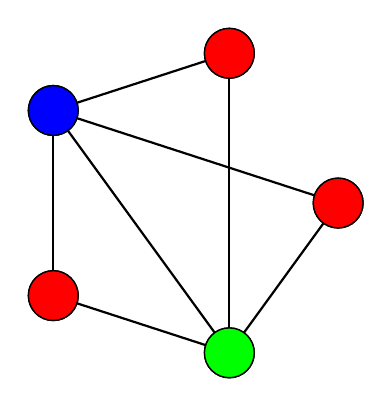
\begin{tikzpicture}
\SetGraphUnit{2}
\Vertices{circle}{A,B,C,D,E}
\Edges(B,C,D,E,A,C,E,B)
\AddVertexColor{red}{B,D,A}
\AddVertexColor{blue}{C}
\AddVertexColor{green}{E}
\end{tikzpicture}
\end{center}

Now we construct a proof without revealing the 3 coloring. Both the Prover and the Verifier can see the graph structure, but only the Prover can see the coloring. The Prover wants to prove that the graph is 3 colorable without revealing the coloring.

First, the Prover will hide all of the colors in the 3 coloring. Say that the Prover covers up each vertex with a piece of paper. They can color in the coloring, but after the paper goes down, the coloring cannot be modified. There is a way to do this cryptographically, which we will discuss later.

Next, the Verifier will give a random challenge, for example, choose two adjacent vertices. The Prover will reveal their colors, and show that they are different colors. Doing so will reveal the colors of some vertices, which is undesirable. Instead, we can map the original colors to a different color, so that whichever colors are revealed are random. We keep the set of colors the same. For example, we can remap the colors as follows.
\begin{align*}
    \text{blue} &\to \text{red}\\
    \text{red} &\to \text{blue}\\
    \text{green} &\to \text{red}
\end{align*}

Checking one edge is not sufficient for the Verifier to be convinced that the graph is 3-colorable. If $G \notin L$, i.e. the graph is not 3-colorable, the probability that the Prover is caught is $\Pr [P^* \text{ is caught}] \geq 1 / |E| $. This is because if the graph is not 3-colorable, then there exists at least 1 edge whose vertices have the same color. The probability of the Verifier picking this edge is $1 / |E|$. There is some probability of catching the Prover, so we can amplify this, i.e. amplifying soundness.

One way to do this is for the Verifier to choose multiple edges. Then the Prover must remap the colors to avoid revealing the original coloring. The process is as follows: the Prover remaps the colors, then the Verifier chooses and edge, and the Prover reveals the colors of the vertices on that edge to show that they have distinct colors. This repeats multiple times, with the Prover remapping the colors randomly each time.

The Verifier is allowed to choose the same edge in multiple iterations. If the graph is not 3-colorable, the Prover might try to cheat by setting two adjacent vertices with the same color after they have been checked. Thus, the Verifier may want to check the same edge again to ensure that the Prover does not do so.

If we repeat this $n$ times, the probability that the Prover $P^*$ survives (not caught) is $$\Pr [P^* \text{ survives}] \leq (1 - 1 / |E|)^n.$$
If we pick $n  = \lambda|E|$, then 
\begin{align*}
    \Pr [P^* \text{ survives}] &\leq (1 - 1 / |E|)^{\lambda |E|} \\
    &\approx (1 / e)^\lambda.
\end{align*}

\subsection{Commitment Scheme}

In the earlier 3-coloring example, the Prover places down a piece of paper on each of the vertices so that the color is hidden and cannot be modified. We discuss a cryptographic protocol that can achieve this, which is called a commitment scheme.

\pseudocodeblock{
    \textbf{Sender} \< \< \textbf{Receiver} \\
    m \in \{0, 1\} \< \< \\[2mm][\hline]
    \text{Commit:} \< \< \\
    r \sample \{0, 1\}^\lambda \< \< \\
    c : = \text{Com}(m; r) \< \sendmessageright*{c} \< \\[2mm][\hline]
    \text{Open:} \< \< \\
    \< \sendmessageright*{(m, r)} \< \text{Verify:} \\
    \< \< c = \text{Com}(m; r)\\
}

There are two properties with this scheme:
\begin{itemize}
    \item \textbf{Hiding:} The commitment of 0 is roughly the same as the commitment of 1, i.e. $\text{Com}(0; r) \approx \text{Com}(1; s)$.
    \item \textbf{Binding:} If one has committed to some message, then later on they can only open up to the message that they have committed. They cannot open up do something else. In other words, it is hard to find $r, s$ such that $\text{Com}(0;r) = \text{Com}(1;s)$.
\end{itemize}

\begin{example}[Hash-based commitment]
Randomly sample $r \sample \{0, 1\}^\lambda$. Then the commitment is $\text{Com}(m;r) := H(r || m)$ for a hash $H$. The hash is modeled as a random oracle.

This commitment scheme hiding because the hash function output appears random. The binding property follows from collision resistance of $H$, which means that it is hard to find two inputs that give the same output.

\end{example}

\begin{example}[Pedersen Commitment]
Take a cyclic group $G$ with order $q$ and generator $g$. Let $h \sample G$ for $h = g^x$ where $x$ is hidden to the sender. $h$ can be generated by the receiver. Then randomly sample $r \sample \ZZ_q$ and the commitment is $\text{Com}(m;r) = g^m \cdot h^r.$

Hiding holds because $h^r$ appears as a random group element, so $g^m \cdot h^r$ is random and can be any group element since $g$ is a generator, sort of like a one-time pad.

Binding follows from the discrete log assumption. If we find two $r_0, r_1 \sample \ZZ_q$ with $\text{Com}(0;r_0) = \text{Com}(1;r_1)$, then

\begin{align*}
    g^0 \cdot h^{r_0} &= c = g^1 \cdot h^{r_1}\\
    h ^{r_0 - r_1} &= g\\
    h &= g^{(r_0 - r_1)^{-1}}
\end{align*}

which essentially solves the Discrete Log problem, which is assumed to be hard. Thus, it is hard to find two such $r_0, r_1$.

\end{example}

\subsection{Zero-Knowledge Proof for Graph 3-Coloring}

Now we give a protocol for a Zero-Knowledge Proof for Graph 3-Coloring.

\textbf{Input:} Graph $G = (V, E)$ with vertices $V$ and edges $E$.

\textbf{Witness:} A coloring $\phi : V \to \{0, 1, 2\}$ that assigns vertices to colors 1, 2, 3.

\pseudocodeblock{
    \textbf{Prover} \< \< \textbf{Verifier}\\
    \text{Randomly sample }\pi : \{0, 1, 2\} \to \{0, 1, 2\} \< \< \\
    \forall v \in V, r_v \sample \{0, 1\}^\lambda, c_v : = \text{Comm}(\pi(\phi(V)); r_v) \< \< \\
    \< \sendmessageright*{\{c_v\}_{v\in V}} \< \\
    \< \< \text{Randomly pick an edge }(u, v) \in E\\
    \< \sendmessageleft*{(u, v)} \< \\
    \text{Open commitments }C_u \text{ and }C_v \< \< \\
    \< \sendmessageright*{
        \alpha = \pi(\phi(u)), r_u\\
        \beta = \pi(\phi(v)), r_v
    } \< \text{Verify:}\\
    \< \< C_u = \text{Comm}(\alpha; r_u)\\
    \< \< C_v = \text{Comm}(\beta; r_v)\\
    \< \< \alpha, \beta \in \{0, 1, 2\}, \alpha \neq \beta
}

This lets us prove all \textsf{NP} languages---we can do a reduction to the 3-coloring and prove it that way. In reality, this is expensive and merely a theoretical result.

\subsection{Circuit Satisfiability}
In reality, many choose another \textsf{NP}-complete language, the circuit satisfiability problem. The language considers an arbitrary boolean circuit which consists of \textsf{AND}, \textsf{XOR} gates. The input are certain values $x$ for input values, and witnesses $w$ are the rest of the wires. The satisfiability problem is whether there exists some $w$ to make the circuit evaluate to $1$. Since the input can be any boolean circuit, this is adaptable and widely used in implementation.

% \Graphic{images/2023-03-14/circuit_sat.png}{0.5}

This circuit model is considered a lot.
\begin{example}[Pre-Image of Hash Function]
    The function is $\mathrm{C}(x,w) = H(w) - x + 1$. The circuit will output $1$ on $w$ such that $H(w) = x$. $w$ here is the pre-image of $x$.

    This allows us to, say, represent SHA as a boolean circuit to prove the pre-image of a hash function.
\end{example}

The intuition of the zero-knowlege proof is similar. Let's say the prover has some input values. The prover will commit to the bit of every wire.

% \Graphic{images/2023-03-14/circuit_sat.png}{0.5}

For example, when a verifier asks to confirm a certain \textsf{XOR} gate, the prover will perform a \emph{small} zero-knowledge proof to prove that that gate was computed correctly. Composing commitments and using sigma protocols from before will allow us to gain the functionality we want.

Let's say
\begin{align*}
    c_1 = \mathrm{Com}(x) \\
    c_2 = \mathrm{Com}(y) \\
    c_3 = \mathrm{Com}(z)
\end{align*}
and $x = y\oplus z$. Using a sigma-\textsf{OR} protocol, we can prove
\[(y = 0, z = 0, x = 0)\ \mathsf{OR}\ (y = 0, z = 1, x = 1)\ \mathsf{OR}\ \cdots\]
This allows us to do ZK-proofs for circuit satisfiability.

\subsubsection{Proof Systems for Circuit Satisfiability}
We discuss the proof systems so far for circuit satisfiability.

% \Graphic{images/2023-03-14/circuit_sat_proof_systems.png}{0.5}

The na\"ive proof is to reveal witness $w$. This is not zero-knowledge, but is non-interactive. Using $\Sigma$-protocols, we have zero-knowledge but not non-interaction. Using the Fiat-Shamir heuristic, we get both zero-knowledge and non-interaction.

For the easiest \textsf{NP} proof, communication requires $O(|w|)$ complexity and the verifier verifies in $O(|c|)$ (linear in number of gates) complexity. For $\Sigma$-protocols, communication requires a commitment to each wire, which is $O(|c|\cdot \lambda)$ (needs a factor of $\lambda$ security parameter), and the verifier also verifies in $O(|c|\cdot \lambda)$. This is the same for NIZK.

\begin{center}
    \begin{tabular}{c|c|c|c}
        & NP & $\Sigma$-Protocol & (Fiat-Shamir) NIZK \\
        Zero-Knowledge & No & Yes & Yes\\
        Non-Interactive & Yes & No & Yes\\
        Communication & $O(|w|)$ & ? & ? \\
        Verifier's computation & $O(|C|)$ & ? & ?\\
    \end{tabular}
\end{center}

\emph{Can we make this proof system more succinct?} Can we have communication and verification complexity to be \emph{sublinear} in $|c|$ and $|w|$?

%!TEX root = ../notes.tex
% Scribe: Sudatta Hor
\section{March 13, 2024}
\label{20240313}

This lecture we cover Succinct Non-Interactive Arguments (SNARGs) and introduce secure multi-party computation.

\subsection{Circuit Satisfiability}
Recall the circuit satisfiability problem. The language considers an arbitrary boolean circuit which consists of \textsf{AND}, \textsf{XOR} gates. The input are certain values $x$ for input values, and witnesses $w$ are the rest of the wires. The satisfiability problem is whether there exists some $w$ to make the circuit evaluate to $1$. Since the input can be any boolean circuit, this is adaptable and widely used in implementation.


This circuit model is considered a lot.
\begin{example}[Pre-Image of Hash Function]
    The function is $\mathrm{C}(x,w) = H(w) - x + 1$. The circuit will output $1$ on $w$ such that $H(w) = x$. $w$ here is the pre-image of $x$.

    This allows us to, say, represent SHA as a boolean circuit to prove the pre-image of a hash function.
\end{example}

The intuition of the zero-knowledge proof is similar. Let's say the prover has some input values. The prover will commit to the bit of every wire.

For example, when a verifier asks to confirm a certain \textsf{XOR} gate, the prover will perform a \emph{small} zero-knowledge proof to prove that that gate was computed correctly. Composing commitments and using sigma protocols from before will allow us to gain the functionality we want.

Let's say
\begin{align*}
    c_1 = \mathrm{Com}(x) \\
    c_2 = \mathrm{Com}(y) \\
    c_3 = \mathrm{Com}(z)
\end{align*}
and $x = y\oplus z$. Using a sigma-\textsf{OR} protocol, we can prove
\[(y = 0, z = 0, x = 0)\ \mathsf{OR}\ (y = 0, z = 1, x = 1)\ \mathsf{OR}\ \cdots\]
This allows us to do ZK-proofs for circuit satisfiability.

\subsubsection{Proof Systems for Circuit Satisfiability}
We discuss the proof systems so far for circuit satisfiability.

\begin{center}
    \begin{tabular}{c|c|c|c}
        & NP & $\Sigma$-Protocol & (Fiat-Shamir) NIZK \\
        Zero-Knowledge & No & Yes & Yes\\
        Non-Interactive & Yes & No & Yes\\
        Communication & $O(|w|)$ & ? & ? \\
        Verifier's computation & $O(|C|)$ & ? & ?\\
    \end{tabular}
\end{center}

The na\"ive proof is to reveal witness $w$. This is not zero-knowledge, but is non-interactive. Using $\Sigma$-protocols, we have zero-knowledge but not non-interaction. Using the Fiat-Shamir heuristic, we get both zero-knowledge and non-interaction.

For the easiest \textsf{NP} proof, communication requires $O(|w|)$ complexity and the verifier verifies in $O(|c|)$ (linear in number of gates) complexity. For $\Sigma$-protocols, communication requires a commitment to each wire, which is $O(|c|\cdot \lambda)$ (needs a factor of $\lambda$ security parameter), and the verifier also verifies in $O(|c|\cdot \lambda)$. This is the same for NIZK.

\emph{Can we make this proof system more succinct?} Can we have communication and verification complexity to be \emph{sublinear} in $|c|$ and $|w|$?

\subsection{Succinct Non-Interactive Argument (SNARG)}
This brings us to succinct arguments, which are seemingly not quite possible.
\begin{definition}[Succinct Non-Interactive Arguments]
    A non-interactive proof/argument system is \ul{succinct} if
    \begin{itemize}
        \item The proof $\pi$ is of length $|\pi| = \mathrm{poly}(\lambda, \log |c|)$.
        \item The verifier runs in time $\mathrm{poly}(\lambda, |x|, \log|c|)$.
    \end{itemize}
\end{definition}
Additionally, SNARKs are Succinct Non-Interactive Arguments of Knowledge. A zk-SNARG or zk-SNARK additionally guarantees zero-knowledge property.

\emph{Why succinct proofs?} Here are some examples where we might want succinct proofs.
\begin{example}[Verifiable Computation]
    The client sends some $x$ to the server, along with function $f$. The server sends back $y = f(x)$ and a proof. The client wants to check if the computation was done correctly.

    \pseudocodeblock{
        \textbf{Server} \< \< \textbf{Client}\\
            \< \sendmessageleft*{x} \< \\
            \< \sendmessageleft*{\text{compute }f} \< \\
            \< \sendmessageright*{y} \< \text{Check }y = f(x)
    }

    If we did not have succinct proofs, then the client would still have to run the function again to verify the output. Note this allows interactions, so this is not the go-to example.
\end{example}
\begin{example}[Anonymous Transactions on Blockchains]
    We think of the blockchain as a public ledger. Say Alice wants to send 2 Bitcoin to Bob, Alice will sign the transaction using her signing key and add that transaction onto the ledger. All transactions are public, you know which addresses sent to which addresses.

    \pseudocodeblock{
        \textbf{Alice's Account A} \< \< \textbf{Bob's Account B}\\
        \text{vk}_A \text{ (public)}, \text{sk}_A \text{ (private)} \< \sendmessageright*{2 \text{BTC (Bitcoin)}} \< \text{vk}_B \text{ (public)}, \text{sk}_B \text{ (private)}\\
        \< \< \\[][\hline]
        \textit{Transaction}\< \< \\
        \sigma = \text{Sign}_{\text{sk}_A} (\text{vk}_A, \text{vk}_B, \text{2 BTC}) \< \sendmessageright*{\sigma}\< \\
        \< \< \\[][\hline]
        \textit{Anonymous Transaction} \< \< \\
        \text{Com}(\sigma) \< \sendmessageright*{ }\< \\
        \text{NIZK: valid transaction} \< \< \\
    }

    There's a lot of work to make transactions anonymous. We'll hide a transaction and hide it, and use a NIZK to prove that it is a valid transaction. We want these proofs to be non-interactive and succinct (we don't want users to spend too long doing verification). This is a major application of SNARK and zk-SNARK
\end{example}

\emph{Is it possible?} This remains as the large problem. Even in the na\"ive \textsf{NP} situation, we need to send the entire witness $w$ and check the entire witness.

Enter probabilistically checkable proofs (PCP):

The prover prepares a proof and the verifier will only need to check certain bits of the proof.

\begin{theorem}[PCP Theorem, Informally]
    Every \textsf{NP} language has a PCP where the verifier reads only a \emph{constant} number of bits of the proof, to gain constant soundness.
\end{theorem}

The intuition is for the prover to commit the entire proof, the verifier checks certain bits, and the prover opens commitments.


The problem with this is that the first round message is not succinct (the commitment is just as long).

Instead of committing linearly, we'll use a Merkle Tree, and only send the commitment/hash of the root node. We build up a binary tree where each node is the hash of its branches. Opening particular bits, the prover will send the root-to-leaf path along with siblings to prove that this opening was correct. This size will grow logarithmically with the size of the tree.

\Graphic{images/2023-03-16/merkle.png}{0.7}

We hash values in a tree format, with each parent node being the hash of its children. We only send the \emph{root note}. Whenever the verifier requests a certain bit, we send the path from the root to the bit (revealing all hashes, and siblings) to verify that this is indeed.

It's very difficult to change any bit. If we changed a bit, at some point up the path of the tree we'll have found a collision for a hash. That is to say, a specific bit being correct is predicated on whether the path to the root is valid and the root hash matches.

\emph{Can we make this hiding?} Right now, we don't guarantee the hiding property. If we only had one layer, every bit would be revealed. How can we modify this algorithm to ensure that each bit is hiding?

One solution would be to add a random string $r$ as a sibling to every leaf. However, this would require us to reveal all siblings when we're verifying a certain leaf node. We can easily modify this to \emph{salt} \emph{every} leaf node. We can add some random $r_i$ to the hash of \emph{every} bit that hides those bits.

Now, instead of sending a commitment of the entire proof, we send a Merkle Tree of the commitment of the proof. Then, when requested for certain bits $i, j, k$, we'll open those commitments as paths on the tree.

\emph{Is this zero-knowledge?} Note that in the PCP theorem, we did not have the zero-knowledge property. Our solution is that when opening commitments, we can instead provide ZK proofs for our `reveals' instead of the actual bits themselves. Asymptotically, this still preserves our succinctness property.

Theoretically, this lets us construct zk-SNARGs. In practice, there are more efficient ways to construct them, but we will not cover them now.

\subsection{Secure Multi-Party Computation}

\subsubsection{2-Party Computation}

We've seen this before, but it is when some parties want to compute the output of some function on their individual inputs, without revealing their own inputs.

\begin{example}
    Alice and Bob just returned from a date, and want to figure out if they each want a second date. Alice has some choice bit $x$ and Bob some choice bit $y$. They want to jointly compute $f(x, y) = x\land y$.
\end{example}
\begin{example}
    Alice and Bob want to compare riches (who is richer?). They compute
    \[f(x, y) = \begin{cases}
            0 & \text{if }x>y    \\
            1 & \text{otherwise}
        \end{cases}\]
\end{example}
\begin{example}
    Alice and Bob meet for the first time and want to see if they have friends in common. They have sets of friends $X,Y$, and compute
    \[f(X, Y) = X\cap Y.\]
    There are variants of this which only give cardinality of $X\cap Y$, etc.
\end{example}

In general, this is when two parties have inputs $x, y$ and want to compute some function $f(x, y)$ on them.

\pseudocodeblock{
    \textbf{Alice}\< \< \textbf{Bob}\\
    \text{Knows x} \< \< \text{Knows y}\\
    \< \< \\
    \< \sendmessageright*{\text{Does computation}} \< \\
    \< \sendmessageleft*{ }\< \\
    \< \sendmessageright*{ }\< \\
    \< \sendmessageleft{bottom={z=f(x,y)}}\< \\
}

Use cases include:
\begin{itemize}
    \item Password breach alert (Chrome/Firefox/Azure/iOS Keychain) runs a set intersection on your passwords and server leaked passwords.
    \item Privacy-preserving contact tracing for COVID-19 (Apple and Google). We want to know if we have contact but not who had contact with.
    \item Ads conversion measurements/personalized advertising (Google/Meta). We want to match conversions without either party knowing who converted.
\end{itemize}

\subsubsection{Multiple Parties!}
The general case of this is Secure Multi-Party Computation (MPC)

\Graphic{images/2023-03-16/mpc.png}{0.4}

This is when we have some parties $P_i$ and want to compute input on $f(x_i, \cdots, x_n)$.

Here are some applications:
\begin{itemize}
    \item Privacy-Preserving Inventory Matching (J.P. Morgan). We have stocks we want to buy/sell but we don't want to reveal which exact ones.
    \item Setup Ceremony to securely generate CRS (Zcash).
    \item Distribute Key Management (Unbound / Coinbase). Instead of holding a secret key on a single device, distribute it among multiple devices/servers. 
    \item Federated learning (used in Google Keyboard Search Suggestion). We want to run machine learning, federated amongst multiple devices. However, we don't want to leak the actual training data from users.
    \item Auctions (Danish sugar beet auction). Nobody should reveal their bid in the clear.
    \item Also deployed in Boston area to analyze the wage gap between genders without revealing the individual salaries.
\end{itemize}
Some applications are still in the works:
\begin{itemize}
    \item Study/Analysis on Medical Data. Every institution has limited data, but they cannot openly share that data due to regulations. How could they jointly do analysis on this data without revealing the data.
    \item Fraud Detection (banks). Users might have cards at multiple banks, they want to jointly detect fraud but do not want to share their transactions.
\end{itemize}

When we normally talk about cryptography, we talk about `slowing down' the system (crypto makes everything slower). In the case of MPC, though, we've enabled new features that were not otherwise possible without these tools.

\subsection{Setting}
Our setting is that we have $n$ parties $P_1, \dots, P_n$ with private inputs $x_1, \dots, x_n$. They want to jointly compute $f(x_1, \dots, x_n)$.

In terms of communication infrastructure: we usually assume point-to-point channels between each pair $(p_i, p_j)$. We know how to do this (key exchange, authenticated encryption, etc). Sometimes, we also assume a reliable broadcast channel where every other party gets information.

There is a single adversary that can ``corrupt'' a subset of the parties (at most $t$).

\emph{What properties do we want out of this system?} Here are some common security properties we might want:
\begin{description}
    \item[Correctness.] The function is computed correctly.
    \item[Privacy.] Only the output is revealed.
    \item[Independence of Inputs.] Parties cannot choose their inputs depending on others' inputs.
\end{description}
Also with security guarantees:
\begin{description}
    \item[Security with Abort.] The adversary may ``abort'' the protocol. This prevents honest parties from receiving the output. This is the weakest model.
    \item[Fairness.] If one party receives the output, then all parties will receive the output.
    \item[Guaranteed Output Delivery (GOD):] Honest parties \emph{always} receive output. Even if adversarial parties leave, the honest parties will simply continue the protocol.
\end{description}

We also have some characterizations of adversaries:
\begin{itemize}
    \item Allowed adversarial behavior:
          \begin{itemize}
              \item Semi-honest (or passive/honest-but-curious): They follow the protocol description honestly, but they try to extract more information by inspecting the transcript. This is the weaker model.
              \item Malicious/active: These adversaries can deviate arbitrarily from protocol description.
          \end{itemize}
    \item Adversary's computing power:
          \begin{itemize}
              \item Unbounded computing power: this gives us information-theoretic (IT) security.
              \item PPT bounded: this gives us computational security.
          \end{itemize}
\end{itemize}

If you're interested, you can look into the literature of how to define security for MPCs. The idea is similar to that of ZK proofs---everything an adversary can do (see the transcript) can be simulated by a simulator who only has the input and output.
%!TEX root = ../notes.tex
% Scribe: Sudatta Hor
\section{March 18, 2024}
\label{20240318}

Some announcements: you can submit a mid-semester feedback form and an intro video, both for extra credit.

This lecture we will cover feasibility results of multi-party computation (MPC), introduce Yao's garbled circuits, and oblivious transfer.

\subsection{Secure Multi-Party Computation, \emph{continued}}
To quickly recap, a two-party computation is a computation where two parties want to jointly compute a function $f(x, y)$ on their private inputs $x, y$---but they do not reveal to each what their inputs are.

In the multi-party case, there will be $n$ parties $P_1, P_2, \dots, P_n$ with inputs $x_1, x_2, \dots, x_n$ wishing to jointly compute $f(x_1, x_2, \dots, x_n)$. We generally assume there are secure point-to-point channels, but some models assume broadcast channels. A single adversary can ``corrupt'' a subset of the parties, say $t$.

Here are properties we wish to attain in our protocol:
\begin{description}
    \item[Correctness.] The function is computed correctly.
    \item[Privacy.] Only the output is revealed.
    \item[Independence of Inputs.] Parties cannot choose their inputs depending on others' inputs.
\end{description}
Also with security guarantees:
\begin{description}
    \item[Security with Abort.] The adversary may ``abort'' the protocol. This prevents honest parties from receiving the output. This is the weakest model.
    \item[Fairness.] If one party receives the output, then all parties will receive the output.
    \item[Guaranteed Output Delivery (GOD):] Honest parties \emph{always} receive output. Even if adversarial parties leave, the honest parties will simply continue the protocol.
\end{description}

\subsection{Feasibility Results}
In the computational security setting, if we have a fundamental building block, a semi-honest oblivious transfer (OT), we can get semi-honest MPC for any function $t<n$. At a high level, using zero-knowledge proofs to enforce correctness of the protocol, we can convert any semi-honest MPC into a malicious MPC.

In terms of information-theoretic (IT) security. We can also get semi-honest and malicious MPC for any function with $t < \frac{n}{2}$. We call this an \ul{honest majority}. This is a necessary bound, we cannot do any better than this.

\subsection{Oblivious Transfer}
\begin{definition}[Oblivious Transfer]
    An \ul{oblivious transfer} is a protocol in which a sender, with messages $m_0, m_1\in\{0, 1\}^l$ gives a choice to the receiver to receive either $m_0, m_1$.

    Given a choice bit from the receiver $b\in\{0,1\}$, the receiver gets $m_b$ and the sender also gets no information about the message transferred.

    % \Graphic{images/2023-03-21/ot.png}{0.6}

    \pseudocodeblock{
        \textbf{Sender} \< \< \textbf{Receiver}\\
        \text{Input: } m_0, m_1 \in \{ 0 , 1\}^{\ell} \< \< \text{Input: } b \in \{0, 1\}\\
        \< \sendmessageright*{ } \< \\
        \< \sendmessageleft*{ }\< \\
        \< \sendmessageright*{ }\< \\
        \< \sendmessageleft*{ } \< \\
        \text{Output: }\perp \< \< \text{Output: }m_b
    }
\end{definition}

We'll learn about constructions of OT later, but we black-box its implementation until later.

Using a semi-honest OT, we can use Yao's Garbled Circuit to construct semi-honest 2PC for any function. We can also use the GMW compiler to compile this into a semi-honest MPC for any function. We'll focus on the first approach in this lecture, but we'll learn GMW in the following lectures.

\subsection{Yao's Garbled Circuit}

\begin{example}[Private Dating/\textsf{AND} Gate]
    Alice and Bob want to figure out whether they want to go on a second date. Alice has single bit $x\in\{0,1\}$, and Bob also has single bit $y\in\{0,1\}$.

    They want to compute a single \textsf{AND} gate.

    Alice will \emph{garble} circuit wires by generating some random $l_0, l_1$ for each wire corresponding to each bit possibility. We call these \emph{labels}.

    \Graphic{images/2023-03-21/yao_private_dating.png}{0.7}
    

    For each \textsf{AND} gate\framedfootnote{We can change the values depending on the different logic gates.}, she'll generate $4$ ciphertexts,
    \begin{align*}
        \Enc_{\alpha_0}(\Enc_{\beta_0}(0)) \\
        \Enc_{\alpha_0}(\Enc_{\beta_1}(0)) \\
        \Enc_{\alpha_1}(\Enc_{\beta_0}(0)) \\
        \Enc_{\alpha_1}(\Enc_{\beta_1}(1))
    \end{align*}

    If we have some $\alpha_a, \beta_b$, then we can decrypt $\Enc_{\alpha_a}(\Enc_{\beta_b}(\cdots))$ and all other ciphertexts will look like garbage (we gain no information). This is to say, we can only decrypt the ciphertext of the keys we know. The overarching idea is that we'll only know the right labels for our inputs.

    Alice will send the circuit (the $4$ encryptions) as well as the input label for $x$, $\alpha_a$. Bob now needs to get the label correponding to his input wire, $\beta_0, \beta_1$. We can perform an oblivious transfer!

    Bob has a choice bit and gets one of $\beta_0, \beta_1$ without Alice knowing his choice bit. Having attained $\beta_b$, Bob will try the encryption on all $4$ ciphertexts with $\alpha_a, \beta_b$, and sees which output is valid and returns that.

    For Alice to learn this output, Bob will send the output back to Alice. In the semi-honest setting, Bob will honestly send the result back to Alice. In the malicious case, we might require Bob to provide some zero-knowledge proof in the end to prove that their plaintext result came from their circuit.
\end{example}

We'll generatlize this single-gate computation for arbitrary functions. We'll represent any arbitrary function as a boolean circuit consisting of only \textsf{AND} and \textsf{XOR} gates\footnote{Recall that any boolean circuit can be represented using only \textsf{AND} and \textsf{XOR} gates.}.

\Graphic{images/2023-03-21/yao_multiple_gates.png}{0.7}

Every wire gets two labels, corresponding to a $0$ bit or $1$ bit. Each label is $\sampledfrom\{0,1\}^\lambda$. For each gate, we construct a `mini' garbled table, where the encrypted message is the output $0$ or $1$ labels\footnote{\emph{How will we know which is garbage?} Na\"ively, we could just try every label. However, this is an exponential blowup for every gate we run the labels through. The solution is to attach a bitstring `tag' (could just be a string of $0$s) that indicates whether a decryption is indeed a label.}\footnote{One more subtle thing we should take care of! We show our ciphertexts in order of $00,01,10,11$. This reveals information! We should take care to shuffle the ciphertexts everywhere.}. We vary the encryptions based on the gate we're trying to implement.

Using the garbled circuit, we can construct an arbitrary 2PC. We call the party who generates the circuit the `garbler', and the other party the `evaluator'.

\Graphic{images/2023-03-21/yao_protocol.png}{0.8}

Alice garbles the circuit, and sends it to Bob. Alice can easily send her own labels. For the labels corresponding to Bob's input, we run oblivious transfer for each input wire to get Bob's input bits without Alice knowing.

In the final output, we can encrypt plaintext $0, 1$. The other way is for Alice to send the final random labels to Bob along with their corresponding bits.

\subsubsection{Optimizations}
There are some optimizations we can make:

\emph{Point-and-Permute.} For each wire, we'll randomly sample signal bits $\sigma_\alpha, \sigma_\beta$, and flip it for the other input. (Note that this doesn't reveal anything about $\alpha,\beta$). In the circuit, we can indicate using the signal bit which ciphertext to decrypt.

\Graphic{images/2023-03-21/point_and_permute.png}{0.7}

We reduce Bob's computation complexity by at least a constant of $4$, and saves communication complexity by half (we don't need to expand our garbled circuit size anymore).

\emph{Row Reduction.} In this construction, there are $4$ ciphertexts per gate. We can just hash the labels and \textsf{XOR} with the corresponding output label (this is not CPA-secure, but that is fine). From the $4$ ciphertexts, we can set $\gamma_0$ to exactly the hash $H(\alpha_0||\beta_0)$\footnote{Not really the $0,0$ labels, but they can correspond to the signal bits.}. This is compatible with point-and-permute. We hide every row, which is fine. This gives us a $\frac{3}{4}$ space decrease.

\Graphic{images/2023-03-21/row_reduction.png}{0.5}

\emph{Free \textsf{XOR}.} Sample a global $\Delta\sampledfrom\{0,1\}^\lambda$. Every pair of labels differ by $\Delta$. That is,
\begin{align*}
    \alpha_1 & :=\alpha_0\oplus \Delta \\
    \beta_1  & :=\beta_0\oplus \Delta  \\
    \gamma_1 & :=\gamma_0\oplus \Delta
\end{align*}
and $\gamma_0 = \alpha_0\oplus \beta_0$. To compute the output label, you just perform the \textsf{XOR} plainly.

This is to say, \textsf{XOR} is free. We don't need to send labels and Bob doesn't need to encrypt/decrypt.

\Graphic{images/2023-03-21/free_or.png}{0.5}

We can also use \emph{half-gates} which give us $2\lambda$ bits per \textsf{AND} gate + free \textsf{XOR}. A recent development, \emph{slicing-and-dicing}, gives us around $\sim 1.5\lambda$ bits per \textsf{AND} gate + free \textsf{XOR}.
%!TEX root = ../notes.tex
% Scribe: Sudatta Hor
\section{March 20, 2024}
\label{20240320}

This lecture we discuss optimizations of garbled circuits, construction of oblivious transfer, semi-honest 2PC, and cut-and-choose for garbled circuits.

\subsection{Oblivious Transfer}

Recall the definition of Oblivious Transfer.

\begin{definition}[Oblivious Transfer]
    An \ul{oblivious transfer} is a protocol in which a sender, with messages $m_0, m_1\in\{0, 1\}^l$ gives a choice to the receiver to receive either $m_0, m_1$.

    Given a choice bit from the receiver $b\in\{0,1\}$, the receiver gets $m_b$ and the sender also gets no information about the message transferred.

    % \Graphic{images/2023-03-21/ot.png}{0.6}

    \pseudocodeblock{
        \textbf{Sender} \< \< \textbf{Receiver}\\
        \text{Input: } m_0, m_1 \in \{ 0 , 1\}^{\ell} \< \< \text{Input: } b \in \{0, 1\}\\
        \< \sendmessageright*{ } \< \\
        \< \sendmessageleft*{ }\< \\
        \< \sendmessageright*{ }\< \\
        \< \sendmessageleft*{ } \< \\
        \text{Output: }\perp \< \< \text{Output: }m_b
    }
\end{definition}

\subsection{Yao's Garbled Circuit for Arbitrary function}

Let's say Alice (Garbler) and Bob (Evaluator) want to jointly compute an arbitrary function, represented by a series of boolean gates. In this series of boolean gates, there are input wires, intermediate gates, and output wires. Alice has two input wires (red) and Bob has two input wires (blue). Their inputs are known to themselves and do not want to be revealed, but they want to jointly compute the output.

\Graphic{images/2023-03-21/yao_multiple_gates.png}{0.7}

For each wire (a-g), Alice will sample two random 128-bit strings $k_0$ and $k_1$. Alice will create a \textit{garbled table} for each gate that consists of 4 ciphertexts that corresponds to the gate logic. For example, the table at the bottom of the diagram corresponds to the AND gate where each entry is $\text{Enc}_x (\text{Enc}_y(x \text{ AND } y))$, where $x,y$ are the strings $k_0, k_1$ corresponding to each input wire.

Bob will get one label per wire, so then he will be able to decrypt exactly 1 out of 4 ciphertexts in the table.

This occurs for each gate. Alice will send a garbled gate (garbled table) for each gate. For the labels that belong to Alice, she will send both to Bob. Then we allow Bob to choose his input labels using oblivious transfer. This allows Bob to compute the output of a gate without Alice or Bob learning each other's input. Once an output for an intermediate gate is computed, we repeat the process to evaluate later gates.

\Graphic{images/2023-03-21/yao_protocol.png}{0.8}

In order to ensure that one does not learn the other's inputs, we must shuffle the garbled table. The plaintext is concatenated with a series of 0s before being encrypted.

\subsubsection{Optimizations}
There are some optimizations we can make:

\emph{Point-and-Permute.} For each wire, we'll randomly sample signal bits $\sigma_\alpha, \sigma_\beta$, and flip it for the other input. (Note that this doesn't reveal anything about $\alpha,\beta$). In the circuit, we can indicate using the signal bit which ciphertext to decrypt.

\Graphic{images/2023-03-21/point_and_permute.png}{0.7}

We reduce Bob's computation complexity by at least a constant of $4$, and saves communication complexity by half (we don't need to expand our garbled circuit size anymore).

\emph{Free \textsf{XOR}.} Sample a global $\Delta\sampledfrom\{0,1\}^\lambda$. Every pair of labels differ by $\Delta$. That is,
\begin{align*}
    \alpha_1 & :=\alpha_0\oplus \Delta \\
    \beta_1  & :=\beta_0\oplus \Delta  \\
    \gamma_1 & :=\gamma_0\oplus \Delta
\end{align*}
and $\gamma_0 = \alpha_0\oplus \beta_0$. To compute the output label, you just perform the \textsf{XOR} plainly.

This is to say, \textsf{XOR} is free. We don't need to send labels and Bob doesn't need to encrypt/decrypt.

\Graphic{images/2023-03-21/free_or.png}{0.5}

We can also use \emph{half-gates} which give us $2\lambda$ bits per \textsf{AND} gate + free \textsf{XOR}. A recent development, \emph{slicing-and-dicing}, gives us around $\sim 1.5\lambda$ bits per \textsf{AND} gate + free \textsf{XOR}.

\subsection{Oblivious Transfer}
We saw last time how to construct Yao's garbled circuit using oblivious transfer, but we black boxed the implementation of OT.

We'll go over the implementation of semi-honest OT here. It will follow similarly to the Diffie-Hellman key exchange.

\Graphic{images/2023-03-23/ot.png}{0.7}

The sender will send $A = g^a$. The receiver will mask $A^c$ with $c\in \{0,1\}$ and $b\sampledfrom \ZZ_q$. $a,b$ here are like Diffie-Hellman privates.

Then, the sender will compute $k_0 := H(B^a), k_1 := H\left( \left( \frac{B}{A} \right)^a \right)$. This means that $k_c$ will be exactly $g^{ab} = A^b$ (whether $c = 0$ or $c = 1$). Then, $k_0$ and $k_1$ will be used to encrypt $m_0, m_1$ respectively.

Since only one will be the shared Diffie-Hellman key (and the other will require knowledge of $a$), the receiver will only be able to reveal one such message.

Doing out the algebra, we can conclude that the receiver can access the key.

\Graphic{images/2023-03-23/ot_steps.png}{0.8}

\emph{Is this secure against a semi-honest receiver?} If the key is $c = 0$, then the other key will be $g^{ab-a^2}$. $g^{a^2}$ is difficult to compute, since the receiver only has $A = g^a$ and will need secret $a$ to compute $g^{a^2}$.\footnote{Formally, this security is guaranteed by the CDH assumption, that if we have $g^{\alpha}, g^{\beta}$, it's computationally hard to determine $g^{\alpha\beta}$. If an adversary can derive $g^{\alpha^2}$ from $g^{\alpha}$, they can also derive $g^{\alpha\beta}$. We can get $g^{\alpha^2}, g^{\beta^2}$, then we can get $g^{(\alpha+\beta)^2}=g^{\alpha^2 + 2\alpha\beta + \beta^2}$ and taking inverses we can peel off the $\alpha^2,\beta^2$ exponents to get $g^{\alpha\beta}$.} If $c = 1$, then the other key will be $g^{a^2 + ab}$ which is hard again. So, for the receiver, it is computationally secure.

\emph{Is this secure against a semi-honest sender?} $g^b$ is a random mask on $A^c$, so the sender will not be able to distinguish between this.

\subsubsection{OT Extension}
We used public-key operations to achieve our OT. Is it possible to construct OT only using symmetric-key primitives? Unlikely\dots

There are impossibility results that show that if we assume $\mathsf{P}\neq \mathsf{NP}$, it's not possible to construct an OT using symmetric-key primitives.

This makes OTs very difficult---since it takes an entire protocol (including expensive exponentiations) to transfer one bit. There has been current research in \emph{extending} OT so we can use more bits.

An OT extension can extend $O(\lambda)$ OTs (with $O(\lambda)$ public-key operations) into a $\mathrm{poly}(\lambda)$ bit OTs.

\Graphic{images/2023-03-23/ot_extension.png}{0.7}

\subsection{Putting it Together: Semi-Honest 2PC}\label{sec:mar23-semihonest-2pc-together}

We can now construct our 2PC protocol. Alice, the garbler, will create the circuit with garbled inputs and wires (shuffling order of ciphertexts). Alice sends this circuit to Bob, and Bob will use OTs with his input bits to get the wire labels that he should use. Then, Bob runs these labels on the garbled circuit.

\Graphic{images/2023-03-23/2pc_protocol.png}{0.8}

In the semi-honest case, Alice will generate this circuit correctly and Bob will follow the protocol correctly. \emph{What could go wrong against malicious adversaries?}
\begin{itemize}
    \item Alice could garble an incorrect gate, or give an entirely incorrect circuit.
    \item Alice could refuse to send the result (translate output label to bits) back to Bob, or send an incorrect result to Bob. If the outputs are not garbled, then Bob could similarly refuse to send this back to Alice.
    \item Alice and Bob could both cheat about their inputs.
\end{itemize}
%!TEX root = ../notes.tex
% Scribe: Sudatta Hor
\section{April 1, 2024}
\label{20240401}

Thank you to everyone who filled out the feedback form! We will briefly go over the feedback and then continue cut-and-choose for garbled circuits and start GMW.

\subsection{Mid-Semester Feedback}

We collected 101 out of 125 student feedback.

\begin{itemize}
    \item Class attendance is good. A majority of students are attending classes. Those who do not attend class watch the recordings, which is perfectly fine.
    \item Lecture pace. Most students find that the pace is fine. We will keep the same pace, but slow down around challenging/technical topics.
    \item Class participation (Q \& A) / Group discussion / Quizzes. We encourage more questions in class, since other students also appreciate those questions. Some students suggest group discussion or quizzes, but we don't want to put pressure on students during lecture.
    \item Diagrams / Reviews / Explanations / Notes / Recordings. Students found the recordings helpful.
    \item Recordings. Panopto recordings are now available! They have better audio quality compared to the Zoom recordings, but they do not have a good audio recording for the audience. The Zoom transcript will be enabled to assist when the audio is not clear.
    \item Examples / Definitions. It may be better to incorporate examples first, and then definitions. This is a good suggestion, and we'll try to incorporate this moving forward.
    \item Docker / Stencil Code / Notation / Local tests / Gradescope. In practice, programming in this field requires using some crypto library (e.g. CryptoPP, Microsoft SEAL). Sometimes in industry, using these libraries can give a lot of issues. The Docker environment helps to remove many systems level issues. Sometimes you will need to figure out how to use libraries that are not well documented, and working with the stencil code in our projects is hopefully good practice for this. The notation indeed can be confusing between the handout and the stencil code, and we will try to fix some of these moving forward.
    \item Theory / Applications. Some students asked for more applications and less theory. We want to emphasize that the theory is there, and the applications exist because of the theory. There is a balance between the two.
    \item Potential future topics. Cryptanalysis, elliptic-curve cryptography, blockchain and cryptocurrencies, anonymous credential, key transparency, post-quantum cryptography, app attestation, Peihan's research / career in cryptography.
\end{itemize}

\subsection{Multi-Party Computation - Big Picture}

There are two different levels of MPC: either semi-honest or malicious. Semi-honest means that the adversary follows the protocol, but tries to extract more information. Malicious means that the adversary deviates from the protocol to extract information.

If we have an oblivious transfer (OT) that is secure against semi-honest adversaries, we can use it with Yao's garbled circuit to achieve semi-honest 2-party computation for any function. Then, with the cut-and-choose with commitments, we can achieve malicious 2-party computation. We will discuss this next.

\begin{align*}
    \text{Semi-honest OT}\ & \underset{\text{Yao's Garbled Circuits}}{\implies}\ \text{Semi-honest 2PC for any function} \\
    & \underset{\text{Cut-and-choose with commitments}}{\implies}\ \text{Malicious 2PC for any function}
\end{align*}

In the last part of this lecture, we will discuss how to use semi-honest OT with GMW to achieve semi-honest multi-party computation, which can be extended to malicious MPC.

\begin{align*}
    \text{Semi-honest OT} \ & \underset{\text{GMW}}{\implies} \text{Semi-honest MPC for any function}\\
    & \underset{\text{GMW Compiler with ZKP}}{\implies} \text{Malicious MPC for any function}
\end{align*}

Recall the definition of Oblivious Transfer.

\begin{definition}[Oblivious Transfer]
    An \ul{oblivious transfer} is a protocol in which a sender, with messages $m_0, m_1\in\{0, 1\}^l$ gives a choice to the receiver to receive either $m_0, m_1$.

    Given a choice bit from the receiver $b\in\{0,1\}$, the receiver gets $m_b$ and the sender also gets no information about the message transferred.

    % \Graphic{images/2023-03-21/ot.png}{0.6}

    \pseudocodeblock{
        \textbf{Sender} \< \< \textbf{Receiver}\\
        \text{Input: } m_0, m_1 \in \{ 0 , 1\}^{\ell} \< \< \text{Input: } b \in \{0, 1\}\\
        \< \sendmessageright*{ } \< \\
        \< \sendmessageleft*{ }\< \\
        \< \sendmessageright*{ }\< \\
        \< \sendmessageleft*{ } \< \\
        \text{Output: }\perp \< \< \text{Output: }m_b
    }
\end{definition}

\subsection{Putting it Together: Semi-Honest 2PC}\label{sec:mar23-semihonest-2pc-together}

Recall our 2PC protocol. Alice, the garbler, will garble each gate by creating a table of ciphertexts corresponding to each combination of input wires. Alice sends each garbled gate to Bob, and Bob will use OTs with his input bits to get the wire labels that he should use. Then, Bob runs these labels on the garbled circuit.

\Graphic{images/2023-03-23/2pc_protocol.png}{0.8}

In the semi-honest case, Alice will generate this circuit correctly and Bob will follow the protocol correctly. Recall what could go wrong against malicious adversaries. Notice that there is not much that Bob can do, but there is a lot that Alice can do.
\begin{itemize}
    \item Alice could garble an incorrect gate, or give an entirely incorrect circuit.
    \item Alice could refuse to send the result (translate output label to bits) back to Bob, or send an incorrect result to Bob. If the outputs are not garbled, then Bob could similarly refuse to send this back to Alice.
    \item Alice and Bob could both cheat about their inputs.
\end{itemize}

\subsection{Cut-and-Choose for Garbled Circuits}

As an initial approach, Alice will garble $\lambda$ circuits, and send those to Bob. Bob will randomly pick all but one for Alice to reveal, and will evaluate on the last garbled circuit.

\pseudocodeblock{
    \textbf{Alice (Garbler)} \< \< \textbf{Bob (Evaluator)}\\
    \text{Prepare } \lambda \text{ many garbled circuits} \< \< \\
    \< \sendmessageright*{\lambda \text{ Garbled Circuits}} \< \\
    \< \sendmessageleft*{\text{Randomly pick }1 \text{ of them}}\< \\
    \< \sendmessageright*{\text{Reveal labels for the GC}}\< \\
    \< \< \text{Verify correctness} \\
    \< \textit{Do 2PC with the remaining GCs} \< \\
    \< \< \text{Take the majority result}
}


If Alice generates 1 bad garbled circuit, then the probability that Alice is caught is $\frac{\lambda - 1}{\lambda} = 1 - \frac{1}{\lambda}$. Which is a small probability, but it's not overwhelming.

Instead, Alice will generate $2\lambda$ garbled circuits, and Bob will pick $\lambda$ circuits. Alice will reveal the selected $\lambda$ circuits, and Bob will evaluate on the remaining $\lambda$ and take a majority.

\pseudocodeblock{
    \textbf{Alice (Garbler)} \< \< \textbf{Bob (Evaluator)}\\
    \text{Prepare } 2 \lambda \text{ many garbled circuits} \< \< \\
    \< \sendmessageright*{2\lambda \text{ Garbled Circuits}} \< \\
    \< \sendmessageleft*{\text{Randomly pick }\lambda \text{ of them}}\< \\
    \< \sendmessageright*{\text{Reveal labels for the } \lambda \text{ GCs}}\< \\
    \< \< \text{Verify correctness} \\
    \< \textit{Do 2PC with the remaining GCs} \< \\
    \< \< \text{Take the majority result}
}

What is the probability that Alice gets caught given that Alice generated $\leq \frac{\lambda}{2}$ garbled circuits incorrectly\footnote{If she generated less than this, then the majority will be correct anyways.}? The probability that Alice passed is
\[\Pr\left[ \text{Alice Passed} \right] = \frac{2\lambda - \frac{\lambda}{2}}{2\lambda}\cdot \frac{2\lambda - \frac{\lambda}{2} - 1}{2\lambda - 1} \cdots \cdot \frac{\frac{\lambda}{2} + 1}{\lambda + 1} \leq \left( \frac{3}{4} \right)^\lambda\]
which is negligible. Then, Alice will fail with high probability.

Note that Bob must always take the majority even if he notices that there is some inconsistency between the garbled circuits. With overwhelming probability, the majority must be correct. There is an attack called ``selective abort'', where whether we abort or not depends on the input. Depending on Bob's input, there may or may not be inconsistency. Thus, if Bob aborts when seeing inconsistency, this reveals to Alice some information about what inputs Bob has. Whether Bob aborts or not depends on his input.

\subsection{GMW} \label{sec:mar23-gmw}

There is another method of multi-party computation that does not used garbled circuits called the Goldreich-Micali-Wigderson (GMW) protocol.

Throughout the protocol, we keep the invariant that for each wire $w$, if the value of the wire is $v^w \in\{0, 1\}$, then the parties hold an \ul{additive secret share} of $v^w$. Each party $P_i$ holds a random share $v_i^w\in\{0,1\}$ such that
\[\bigoplus_{i=1}^n v_i^w = v^w\]
and we keep this invariant throughout the entire circuit. \footnote{Recall that $\oplus$ means addition modulo 2. You can check that this also gives the XOR operation.}

We need to be able to preserve this invariant throughout \textsf{AND} and \textsf{XOR} gates. The \textsf{XOR} case is easy, since \textsf{XOR} is completely commutative and associative, so each party can locally \textsf{XOR} their shares $c_i := a_i\oplus b_i$ for $c := a\oplus b$.

We'll wave our hands over the \textsf{AND} case, but we can do this. We'll proceede gate-by-gate for everyone to compute the result. Each party will publish their local shares, and everyone will \textsf{XOR} the result together to get the final result.

\subsubsection{AND Gates}
We now finish addressing the \textsf{AND} gates. We have $\bigoplus^n_{i=1}a_i = a$ and $\bigoplus^n_{i=1}b_i = b$.

We want a set of $\left\{ c_i \right\}$ s.t. $\bigoplus^n_{i=1}c_i = c = a \cdot b$ (multiplication of bits is \textsf{AND}). But
\begin{align*}
    a\cdot b
     & = \left( \sum^n_{i=1}a_i \right)\cdot \left( \sum^n_{i=1}b_i \right)\pmod{2}                \\
     & = \left( \sum^n_{i=1}a_i\cdot b_i \right)\cdot \left( \sum_{i\neq j}a_i b_i \right)\pmod{2}
\end{align*}
The first sum is easy and computed locally, but the second sum requires parties to communicate. We do something called \ul{resharing}.

\textbf{Goal:} Between $P_i, P_j$, we want random $r_i, r_j\in\{0, 1\}$ such that $r_i + r_j = a_i \cdot b_j \pmod{2}$.

$P_i$ will randomly sample $r_i\sampledfrom \left\{ 0, 1 \right\}$. We can use OT to allow $P_j$ to learn $r_j$ such that $r_i + r_j = a_i\cdot b_j\pmod{2}$ without revealing $a_i$ or $r_i$.

$P_i$ will be the sender, $P_j$ is the receiver. $P_j$'s choice bit is $b_j$. Then the messages will be
\begin{align*}
    m_0 & = (a_i\cdot 0) - r_i \\
    m_1 & = (a_i\cdot 1) - r_i
\end{align*}
such that $r_i, r_j$ are two shares of $a_i\cdot b_j$.

\pseudocodeblock{
    \textbf{Party i} \< \< \textbf{Party j}\\
    \text{Input: } a_i \in \{ 0 , 1\} \< \< \text{Input: } b_j \in \{0, 1\} \\
    r_i \sample \{0, 1\} \< \< \\
    \text{Prepare both possibilities for }r_j \< \< \\
    \< \sendmessageleft*{} \< \\
    \< \sendmessageright*{\text{Use OT with choice bit }b_j} \< \\
    \< \< \text{Receive } r_j\\
    \text{Output: }r_i \in \{0, 1\}\< \< \text{Output: }r_j \in \{0, 1\}
}
%!TEX root = ../notes.tex
% Scribe: Sudatta Hor
\section{April 3, 2024}
\label{20240403}

This lecture we will finish our discussion on the GMW protocol. We recap the semi-honest protocol and see how we can construct a malicious secure protocol. In practice, we may want to consider the exact function the we are computing in MPC to enable more efficient protocols. We will discuss an example of this known as Private Set Intersection.

\subsection{GMW}

Recall the Goldreich-Micali-Wigderson (GMW) protocol for multi-party computation.

Throughout the protocol, for each wire $w$, if the value of the wire is $v^w \in\{0, 1\}$, then the parties hold an \ul{additive secret share} of $v^w$. Each party $P_i$ holds a random share $v_i^w\in\{0,1\}$ such that
\[\bigoplus_{i=1}^n v_i^w = v^w\]
and we keep this invariant throughout the entire circuit. \footnote{Recall that $\oplus$ means addition modulo 2. You can check that this also gives the XOR operation.}

We need to be able to preserve this invariant throughout \textsf{AND} and \textsf{XOR} gates. The \textsf{XOR} case is easy, since \textsf{XOR} is completely commutative and associative, so each party can locally \textsf{XOR} their shares $c_i := a_i\oplus b_i$ for $c := a\oplus b$.

We'll wave our hands over the \textsf{AND} case, but we can do this. We'll proceed gate-by-gate for everyone to compute the result. Each party will publish their local shares, and everyone will \textsf{XOR} the result together to get the final result.

\begin{remark}
    \textbf{(Frequently asked)} Why do we only consider AND and XOR gates? This is because every other gate (NOT, OR, NAND) can be constructed using only AND and XOR gates. Gates like this are considered \textbf{complete}.
\end{remark}

\subsubsection{AND Gates}
We now finish addressing the \textsf{AND} gates. We have $\bigoplus^n_{i=1}a_i = a$ and $\bigoplus^n_{i=1}b_i = b$.

We want a set of $\left\{ c_i \right\}$ s.t. $\bigoplus^n_{i=1}c_i = c = a \cdot b$ (multiplication of bits is \textsf{AND}). But
\begin{align*}
    a\cdot b
     & = \left( \sum^n_{i=1}a_i \right)\cdot \left( \sum^n_{i=1}b_i \right)\pmod{2}                \\
     & = \left( \sum^n_{i=1}a_i \cdot b_i \right) + \left( \sum_{i\neq j}a_i \cdot b_j \right)\pmod{2}
\end{align*}
The first sum is easy and computed locally, but the second sum requires parties to communicate. We do something called \ul{resharing}.

\textbf{Goal:} Between $P_i, P_j$, we want random $r_i, r_j\in\{0, 1\}$ such that $r_i + r_j = a_i \cdot b_j \pmod{2}$.

$P_i$ will randomly sample $r_i\sampledfrom \left\{ 0, 1 \right\}$. We can use OT to allow $P_j$ to learn $r_j$ such that $r_i + r_j = a_i\cdot b_j\pmod{2}$ without revealing $a_i$ or $r_i$.

$P_i$ will be the sender, $P_j$ is the receiver. $P_j$'s choice bit is $b_j$. Then the messages will be
\begin{align*}
    m_0 & = (a_i\cdot 0) - r_i = r_i \mod 2\\
    m_1 & = (a_i\cdot 1) - r_i = a_i + r_i \mod 2
\end{align*}
such that $r_i, r_j$ are two shares of $a_i\cdot b_j$.

\pseudocodeblock{
    \textbf{Party i} \< \< \textbf{Party j}\\
    \text{Input: } a_i \in \{ 0 , 1\} \< \< \text{Input: } b_j \in \{0, 1\} \\
    r_i \sample \{0, 1\} \< \< \\
    \text{Prepare both possibilities for }r_j \< \< \\
    \< \sendmessageleft*{} \< \\
    \< \sendmessageright*{\text{Use OT with choice bit }b_j} \< \\
    \< \< \text{Receive } r_j\\
    \text{Output: }r_i \in \{0, 1\}\< \< \text{Output: }r_j \in \{0, 1\}
}

\subsubsection{Complexities}
Computational complexity is $O(\#\mathsf{AND}\cdot n)$ for each party, since each XOR gate takes constant number of operations and each AND gates requires a constant number of operations for each other party.

For communication complexity, each party needs to communicate to every other party for every \textsf{AND} gate. For each XOR gate, we do not need to communicate. So the communication complexity is $O(n \cdot \#\mathsf{AND})$ per party.

The round complexity is the depth of the AND gates in circuit. Each party needs to communicate to every other party for each AND gate, but some of these AND gates can be done in parallel (if they do not depend on each other). Thus, the round complexity is $O(\text{depth of AND gates})$.

\begin{center}
\begin{tabular}{c|c} 
Computational Complexity & $O(\#\mathsf{AND}\cdot n)$ per party\\
Communication Complexity & $O(n^2\cdot \#\mathsf{AND})$\\
Round Complexity & $O(\text{depth of AND gates})$
\end{tabular}
\end{center}

\subsubsection{Malicious adversaries}

So far, the GMW protocol is secure against semi-honest adversaries, who follows the protocol. What could go wrong against malicious adversaries?

\begin{itemize}
    \item Adversaries can share their wrong shares, and do not give the correct output. Essentially, they lie about their input. In MPC, there is no way to prevent this, since each party has the power to choose their input. In general, we do not worry about this at the input level.
    \item In the reshare, adversaries can give an incorrect $a_i$.
\end{itemize}

Next, we will use ZKP to prevent malicious behavior. The high-level idea is the following: given a semi-honest protocol, the protocol is deterministic after fixing the inputs and the randomness.

\begin{itemize}
    \item[Step 1.] Each party $P_i$ commits to its input $x_i$ and randomness $r_i$ to be used in the semi-honest protocol
    \item[Step 2.] Run semi-honest protocol. Along with every message, prove in zero-knowledge that the message is computed correctly based on the input, randomness, and transcript so far.
\end{itemize}

Recall that once a party commits a value, they cannot change that value. Thus, this procedure ensures that no party changes their inputs during the protocol.

\subsection{Yao's Garbled Circuits Vs. GMW}

We have two protocols for MPC: Yao's garbled circuits and GMW.

\begin{center}
\begin{tabular}{c|c}
    \textbf{Yao's Garbled Circuits} & \textbf{GMW} \\
    \hline \\
    2-party computation & $n$-party computation \\
    Round complexity $O(1)$ & Round complexity $O(\text{depth of AND gates})$  \\
    Computation/communication & roughly same \\
    Malicious security uses cut-and-choose, more efficient & Malicious security uses ZKP, not efficient\\
    Only boolean circuits & Can be extended to arithmetic circuits
\end{tabular}
\end{center}

In theory, zero-knowledge proofs can be done for any NP language, because any such language can be reduced into a 3-coloring problem. However, such a reduction is not easy, so in practice, zero-knowledge proofs are expensive for general problems. It is polynomial time, but not efficient.

In general, neither of these are efficient enough. We need to consider the specific function that we are computing to construct a protocol that is more efficient. Next, we will consider an example of such a protocol.

\subsection{Private Set Intersection (PSI)}

Alice and Bob want to compute the intersection of their sets $X = \{x_1, x_2, \dots, x_n\}$ and $Y = \{y_1, y_2, \cdots, y_n\}$ without revealing the elements in their set.

\begin{itemize}
    \item PSI: $f(X, Y) = X\cap Y$.
    \item PSI-Cardinality: $f(X, Y) = |X\cap Y|$ which counts the number of items in the intersection without revealing the items.
\end{itemize}

\textbf{Applications:}
\begin{itemize}
    \item \textbf{Password Breach Alert} (Chrome, Edge, Firefox, iOS Keychain, ...). There is a set of all compromised passwords, and a set of user's passwords, and we want to see if there is intersection without revealing the passwords.
    \item \textbf{Ads Conversion Measurement} (Google). Alice is an ad platform and Bob is an advertiser who has the information of users that have a made a purchase with him. The intersection is the ad conversion, those users who have seen the ads and made a purchase, which gives an idea of the effectiveness of the ad.
    \item \textbf{Privacy-Preserving Inventory Matching} (J.P. Morgan). There is a set of stocks we can sell, and a set of stocks that a buyer wants to buy. We want to which stocks we can sell to the buyer.
    \item \textbf{Private Database Joins.} For example, two companies may want to find out how many users they have in common.
\end{itemize}

\subsubsection{Na\"ive Solution}
Here's a na\"ive solution: Alice and Bob hash all their inputs, exchange hash values, and see which ones they have in common. You can learn the intersection, but could you learn \emph{more} than that?

\pseudocodeblock{
    \textbf{Alice} \< \< \textbf{Bob}\\
    \text{Input: } X = \{x_1, \dots, x_n\} \< \< \text{Input: }Y = \{y_1, \dots, y_n\}\\
    \< \sendmessageright*{H(x_1), \dots, H(x_n)} \< \\
    \< \< \text{Compute intersection between} \\
    \< \< H(x_1), \dots, H(x_n) \text{ and}\\
    \< \< H(y_1), \dots, H(y_n)
}

If the input space is a relatively small space, we can do a dictionary attack (for example, with names). This is not even semi-honest secure.

\emph{Can we even achieve 2PC/MPC with just a single round of communication (as we have done here, sending hashes one way)?} Taking a step back, we receive a message from Alice and can derive the solution regardless of \emph{any} $y$ we have. This allows us to just test multiple inputs on the function received and we'll receive that output, so we can derive $x$ from that input. Thus, no, we cannot achieve 2PC/MPC with just a single round.

\subsubsection{DDH-Based PSI}\label{sec:apr04-psi-ddh}
We start with a cyclic group $\GG$ of order $q$ with generator $g$, where DDH holds. We also have a hash function $H: \left\{ 0, 1 \right\}^{*}\to \GG$ (modeled as a random oracle).

\pseudocodeblock{
    \textbf{Alice:} \< \< \textbf{Bob:}\\
    \text{Input: } X = \{x_1, \dots, x_n\} \< \< \text{Input: }Y = \{y_1, \dots, y_n\} \\
    a \sample \ZZ_q \< \< b \sample \ZZ_q \\
    \< \sendmessageleft*{H(Y)^b := \{H(y_1)^b, \dots, H(y_n)^b\}} \< \\
    \< \sendmessageright*{H(X)^a, H(Y)^{a\cdot b}} \< \\
    \< \< \text{Compute the intersection}\\
    \< \< H(X)^{a\cdot b} \cap H(Y)^{a \cdot b}\\
}

Bob and Alice generate private exponents $k_B\sampledfrom \ZZ_q, k_A\sampledfrom \ZZ_q$ respectively. Bob will send
\[H(Y)^{k_B} := \left\{ H(y_1)^{k_B}, \cdots, H(y_n)^{k_B} \right\}\]
Alice does the same for $X$, $H(X)^{k_A}$, and sends $H(Y)^{k_A\cdots k_B}$. Bob then raises $H(X)^{k_A}$ to $k_B$ and compares. In the semi-honest case, for Bob to perform the same dictionary attack, Bob will need to break DDH in order to raise arbitrary elements $y'$ to $k_A\cdot k_B$.

We can modify this to count cardinality by randomly shuffling the returned $H(Y)^{k_A\cdot k_B}$ such that Bob cannot relate the re-encrypted hashes to the previous order.

% \Graphic{images/2023-04-04/ddh_psi-ca.png}{0.7}

%!TEX root = ../notes.tex
% Scribe: Sudatta Hor
\section{April 8, 2024}
\label{20240408}

In this lecture, we give a brief introduction to Fully Homomorphic Encryption. Then we give a concrete construction of Somewhat Homomorphic Encryption over Integers. We want to use more solid assumptions, so we introduce a new assumption called Learning with Errors, which is a post-quantum assumption, i.e. it is secure against known quantum attacks.

\subsection{Fully Homomorphic Encryption (FHE)}

So far, our encryption schemes primarily follow an ``all-or-nothing'' idea, where if we have the secret key we can decrypt, otherwise we cannot decrypt.

In Homomorphic schemes, we want to have the additional property that an encryption of an input $x$ can be evaluated with a function $f$ to get an encryption of the output $f(x)$ without having to decrypt first.

\begin{center}
\begin{bbrenv}{fhe-box-diagram}
\begin{bbrbox}[name=Eval, namepos=center]
\end{bbrbox}
\bbrmsgto{side=Enc($x$)}
\bbrmsgto{side=$f$}
\bbrqryto{side=Enc($f(x)$)}
\end{bbrenv}
\end{center}

An additively homomorphic scheme means we can combine $\Enc(m_1)$ and $\Enc(m_2)$ to get
\[\Enc(m_1 + m_2)\]
as we saw in Exponential ElGamal or Paillier.

Similarly, we can have a multiplicatively homomorphic scheme which means we can combine $\Enc(m_1)$ and $\Enc(m_2)$ to get
\[\Enc(m_1 \cdot m_2)\]
as we saw in ElGamal or RSA.

Fully homomorphic encryption means we can get both $\Enc(m_1 \cdot m_2)$ and $\Enc(m_1 + m_2)$.

\subsection{Applications}
\begin{example}[Oursourcing Storage \& Computation]
    Let's say a client stores some data on a server. A client has data $x$ and key $sk$. $ct\leftarrow\Enc(x)$ is sent to the server. If the client wants to run some computation on the server, the client sends $f$ and the server evaluates $ct' \leftarrow \mathsf{Eval}(f, ct)$ and sends $ct'$ to the client, which gives the client $f(x)$ without the server knowing $x$.
    
    \pseudocodeblock{
        \textbf{Server} \< \< \textbf{Client}\\
        \< \< \text{Data } x\\
        \< \< \text{Key sk} \\
        \< \< \text{ct} \gets \text{Enc}(x)\\
        \< \sendmessageleft*{\text{ct}, f} \< \\
        \text{ct}' \gets \text{Eval}(f, \text{ct}) \< \< \\
        \< \sendmessageright*{\text{ct}'} \< \\
        \< \< f(x) \gets \text{Dec}_{\text{sk}}(\text{ct}')
    }
\end{example}

\begin{example}[Privacy-Preserving Query]
    The client wants to make a query to the server, e.g. Google search or GPT-4. However, the client does not want to reveal what their query is. Thus, the client encrypts their query and the server homomorphically processes the query and sends back the evaluated ciphertext ct$'$, so that the client gets the query result and teh server does not know the query.

    \pseudocodeblock{
        \textbf{Server} \< \< \textbf{Client}\\
        \< \< \text{Query } x\\
        \< \< \text{Key sk} \\
        \< \< \text{ct} \gets \text{Enc}(x)\\
        \< \sendmessageleft*{\text{ct}} \< \\
        \text{ct}' \gets \text{Eval}(f, \text{ct}) \< \< \\
        f \text{ can be Search, ML, GPT, etc.}\< \< \\
        \< \sendmessageright*{\text{ct}'} \< \\
        \< \< f(x) \gets \text{Dec}_{\text{sk}}(\text{ct}')
    }
\end{example}

\begin{example}[Private Information Retrieval (PIR)]
    In this application (We'll implement this in the next project!), we have some server with a database. A client wants to retrieve the $i$-th element without revealing the index $i$ to the server.

    \pseudocodeblock{
        \textbf{Server} \< \< \textbf{Client}\\
        \text{Database }D \< \< \text{Want: }D[i] \text{ while hiding }i \text{ from the server}\\
        \< \< \text{Query: } i\\
        \< \< \text{Key: sk}\\
        \< \sendmessageleft*{\text{ct}} \< \text{ct} \gets \Enc(i)\\
        \text{ct}' \gets \text{Eval}(f, \text{ct}) \< \< \\
        \text{where }f(i) = D[i] \< \< \\
        \< \sendmessageright*{\text{ct}'} \< \\
        \< \<  D[i] \gets \Dec_{\text{sk}}(\text{ct}')\\
    }

    Note two differences from 1-out-of-$n$ OT.
    \begin{itemize}
        \item \textbf{Security:} In 1-out-of-$n$ OT, the server does not want to reveal any information about their database other than the 1 out of $n$ chosen entry. However, in PIR, we do not enforce such security. In PIR, we allow that the client may learn something else about the database from the ciphertext ct$'$ other than the desired result $f(x)$.
        \item \textbf{Efficiency:} In 1-out-of-$n$ OT, the server will generate $n$ ciphertexts and send them to the client. However, in PIR, we want to be more succinct and only send one ciphertext.
    \end{itemize}

    A na\"ive solution is for the server to send the \emph{entire} database to the client and the client can just access their desired element. In fact, this is the best we can do information-theoretically.

\end{example}

\begin{example}[Secure 2PC]
    As we've seen before, Alice and Bob have some $x, y$ and want to compute $c(x,y)$ privately. Bob encrypts $y$ as $ct\leftarrow \Enc(y)$ and Alice sends $ct' \leftarrow \mathsf{Eval}(f_x, ct)$ with $f_x(y) = c(x,y)$ and sends $ct'$ back to Bob, which he can $\Dec_{sk}(ct')\to f(y)$.

    \pseudocodeblock{
        \textbf{Alice} \< \< \textbf{Bob}\\
        \text{Input: } x\< \< \text{Input: }y\\
        \< \< \text{Key sk}\\
        \< \< \text{ct} \gets \Enc(y)\\
        \< \sendmessageleft*{\text{ct}}\< \\
        \text{ct}'\gets \text{Eval}(f, \text{ct}) \< \< \\
        \text{where }f(y) = C(x, y) \< \< \\
        \< \sendmessageright*{\text{ct}'} \< \\
        \< \< C(x,y) \gets \Dec_\text{sk}(\text{ct}')\\
    }
    \emph{Is this secure?} This is secure against Alice, since she only sees a ciphertext which is guarded by the guarantees of the encryption. Is this secure against Bob? This is not guaranteed. Bob might be able to infer more information about $f$ from ct$'$. It's not necessarily the case that FHE hides the function.
\end{example}

\subsection{FHE Definition}

\begin{definition}[Homomorphic Encryption]\label{def:fhe}
    A (public-key) homomorphic encryption scheme is some
    \[\pi = (\mathsf{KeyGen}, \Enc, \Dec, \mathsf{Eval})\]
    with respect to some function family $\mathcal{F}$ with
    \begin{itemize}
        \item $(pk, sk)\leftarrow \mathsf{KeyGen}(1^\lambda)$.
        \item $ct\leftarrow \Enc_{pk}(m)\qquad m\in \{0, 1\}$.
        \item $m\leftarrow \Dec_{sk}(ct)$.
        \item $ct_f\leftarrow \mathsf{Eval}(f, ct_1, \dots, ct_n)$ with $f : \{0, 1\}^n\to \{0, 1\}$ in family $\mathcal{F}$.
    \end{itemize}

    \textbf{Correctness} requires that $\forall f\in \mathcal{F}$, if $ct_f \leftarrow \mathsf{Eval}(f, ct_1, \dots, ct_n)$ for $ct_i\leftarrow \Enc_{pk}(m_i)$, then $\Dec_{sk}(ct_f) = f(m_1, \dots, m_n)$. That is, that evaluating functions does indeed give the ciphertext of the function evaluated on the plaintexts.

    \textbf{CPA security}, as we've seen before, requires that
    \[(pk, \Enc_{pk}(m_0))\overset{c}{\simeq}(pk, \Enc_{pk}(m_1)).\]
    
    \textbf{Compactness}, that $|ct_f| \leq \mathsf{poly}(\lambda)$, that each ciphertext is bounded by some constant that is polynomial in $\lambda$ and fixed for security parameter $\lambda$. This allows us to prevent the `loophole' of evaluations returning itself.
\end{definition}

\textit{Why do we need compactness?} If we just have correctness and CPA security, our current definition is nearly trivial. For example, if our evaluation just output the tuple $(f, ct_1, \dots, ct_n)$. To decrypt, we decrypt each $ct_i$ individually and apply $f$ on top, and this satisfies our definitions! We need to add some notion that our ciphertext must stay within some size, and that we're actually \emph{combining} our ciphertexts.

If the family of functions $\mathcal{F}$ contains all polynomial sized Boolean circuits, we say that the scheme is \textbf{fully} homomorphic.

\subsubsection{Constructions}
All FHE constructions follow two steps:
\begin{enumerate}
    \item Somewhat Homomorphic Encryption (SWHE). We'll see versions over integers, from LWE (GSW), and from RLWE (BFV).
    \item Then, we bootstrap our SWHE schemes to be fully homomorphic.
\end{enumerate}

\subsubsection{SWHE over Integers}\label{sec:apr06-swhe-integers}
\textbf{Attempt 1.} This is our first attempt is a secret-key scheme:

Our secret key will be odd $p$.

\begin{remark}
    \textit{Why must $p$ be odd?} If $p$ is even, then the ciphertext $p\cdot q + m$ has the same parity as $m$. The message is not secure because we can find it just by checking even/odd. If $p$ is odd, then $p\cdot q$ can be either even or odd, so the parity of the ciphertext is not solely determined by parity of $m$.
\end{remark}

\begin{itemize}
    \item To $\Enc(m)$ with $m\in \{0, 1\}$, we sample a random $q$ and compute $ct = p\cdot q + m$. Encryption of $0$ is a multiple of $p$.
    \item Decryption is $ct\mod p$.
    \item Add: $\text{ct} \gets \text{ct}_1 + \text{ct}_2$.
    \item Multiply: $\text{ct} \gets \text{ct}_1 \cdot \text{ct}_2 $.
\end{itemize}

\emph{Is this CPA secure?} No! If we have a lot of encryptions of $0$s, taking the gcd of them will give us $p$ exactly.

\textbf{Attempt 2.} Our next attempt is to add a small error noise.

\begin{itemize}
    \item To encrypt, instead of $ct = p\cdot q + m$, we'll do
          \[ct = p\cdot q + m + 2e\]
          for small even $2e$ with $e \ll p$. Encryption of $0$ is small and even modulo $p$.
    \item Then, decryption becomes $\Dec(ct) = \left[ ct\mod p \right]\mod 2$.
    \item Addition and multiplication work the same way. Check that the decryption gives the correct result by modding p then modding 2. If
    \begin{align*}
        \text{ct}_1 &= p \cdot q_1 + m_1 + 2e_1 \\
        \text{ct}_2 &= p \cdot q_2 + m_2 + 2e_2 \\
    \end{align*}
    then
    \begin{align*}
        \text{ct}_1 + \text{ct}_2 &= p(q_1 + q_2) + (m_1 + m_2) + (2e_1 + 2e_2)\\
        \text{ct}_1 \cdot \text{ct}_2 &= pq_1(pq_2 + m_2 + 2e_2) + m_1 \cdot pq_2 + m_1 \cdot m_2\\
        & \quad + m_1 \cdot 2e_2 + 2e_1(pq_2 + m_2 + 2e_2)\\
    \end{align*}
\end{itemize}



\textbf{Attempt 3.} We can also construct a public key version of this, where the secret key is still our odd $p$ but the public key are a set of encryptions of $0$, $\{x_i = p\cdot q_i + 2e_i\}$.

Since our scheme is homomorphic over addition, we can take a random subset sum of $\{x_i\}$ and add $m$ and $2e$:
\begin{itemize}
    \item To encrypt, we'll do
          \[ct = (\text{subset sum of $\{x_i\}$}) + m + 2e\]
          for small even $2e$ with $e \ll p$. Encryption of $0$ is small and even modulo $p$.
    \item Then, decryption becomes $\Dec(ct) = \left[ ct\mod p \right]\mod 2$.
    \item Addition and multiplication work the same way.
\end{itemize}

\emph{What could go wrong?} Note that this is still only a \emph{somewhat} homomorphic encryption scheme. Are there limits to how much we can add or multiply? Specifically, could the noise grow to an extent that interferes with our encryption?
\begin{enumerate}
    \item If we add ciphertexts, our noise grows linearly:
          \begin{align*}
              ct_1        & = p\cdot q_1 + m_1 + 2e_1                         \\
              ct_2        & = p\cdot q_2 + m_2 + 2e_2                         \\
              ct_1 + ct_2 & = p\cdot (q_1 + q_2) + (m_1 + m_2) + 2(e_1 + e_2)
          \end{align*}
    \item If we multiply ciphertexts, our noise grows exponentially:
          \[ct_1 \cdot ct_2 = p\cdot (\cdots) + (m_1 \cdot m_2) + m_1\cdot 2e_2 + 2e_1m_2 + 4e_1e_2\]
\end{enumerate}
Addition is cheaper, but multiplication has our noise grow much much faster. In our parameters, we can support roughly $O(\lambda)$ multiplications, but addition is almost for free (we can do exponentially many additions).

This is why this is \emph{somewhat} homomorphic encryption---if the noise exceeds $p$, then it might affect the plaintext.

This analysis works similarly for public-key encryption\footnote{In fact, we took a very generic way of converting the secret-key scheme into a public-key scheme. We can always take subset sums of encryptions of $0$ and add it to our message.}.

Note that this protocol is quite expensive---$p$ and $q$ will tend to get quite large. We'll pivot into lattice-based cryptography which will solve some of these issues.

\subsection{Learning With Errors (LWE) Assumption}
We'll introduce a new assumption, and which is assumed to be post-quantum secure. There is no known quantum algorithm to solve this in polynomial time.

We have security parameter $n$, and $q\sim 2^{n^\epsilon}$ for constant $\epsilon$. $m = \Theta(n\log q)$. We have some distribution $\chi$ which is a distribution over $\ZZ_q$ concentrated on ``small integers''. For example, this can be Gaussian.

% \Graphic{images/2023-04-11/gaussian.png}{0.7}

We require that for $e\sample \chi$, 
\[\Pr[|e| < \alpha\cdot q ]\simeq 1\]
with $\alpha \ll 1$. That is, the probability that our error deviates significantly from $0$ is negligible.

The assumption states the following: sampling a random matrix $A\sampledfrom \ZZ_q^{m\times n}$ and randomly sample a vector $s\sampledfrom \ZZ_q^n$ with error $e\sampledfrom \chi^m$. We have \[b:=A\times s + e\]
% \Graphic{images/2023-04-11/lwe.png}{0.7}

The computational assumption is that
\[(A, b)\overset{c}{\simeq} (A, b')\]
for $b'\sampledfrom \ZZ_q^m$. That is, $(A, b)$ is indistinguishable from a truly random $(A, b')$.


%!TEX root = ../notes.tex
% Scribe: Sudatta Hor
\section{April 10, 2024}
\label{20240410}

\begin{remark}
    \textbf{News!} Avi Wigderson received the Turing award! \href{https://awards.acm.org/about/2023-turing}{Article.} We have seen some of his work e.g.
    \begin{enumerate}
        \item GM{\color{red}W}: ZKP for 3-coloring (All-NP)
        \item GM{\color{red}W}: MPC for any function
    \end{enumerate}
\end{remark}

This lecture, we will continue the Learning with Errors assumption, which is assumed to be a post-quantum assumption. We will see an encryption scheme using this assumption called Regev Encryption. Then we will see another homomorphic encryption scheme called BFV. We put this all together for our next project on Private Information Retrieval (PIR).

\subsection{Learning With Errors (LWE) Assumption}
Recall the Learning with Errors (LWE) assumption from the previous lecture, which is assumed to be post-quantum secure. There is no known quantum algorithm to solve this in polynomial time.

We have security parameter $n$, and $q\sim 2^{n^\epsilon}$ for constant $\epsilon$. $m = \Omega (n\log q)$. We have some distribution $\chi$ which is a distribution over $\ZZ_q$ concentrated on ``small integers''. For example, this can be Gaussian.

\begin{center}
\def\svgwidth{0.5\columnwidth}
\input{images/2024/.xdp-2024-04-10-chi.pdf_tex-S0vhZX}
\end{center}

We require that for $e\sample \chi$, 
\[\Pr[|e| < \alpha\cdot q ]\simeq 1\]
with $\alpha \ll 1$. That is, the probability that our error deviates significantly from $0$ is negligible.

The assumption states the following: sampling a random matrix $A\sampledfrom \ZZ_q^{m\times n}$ and randomly sample a vector $s\sampledfrom \ZZ_q^n$ with error $e\sampledfrom \chi^m$. We have \[b:=A\times s + e\]

The computational assumption is that
\[(A, b)\overset{c}{\simeq} (A, b')\]
for $b'\sampledfrom \ZZ_q^m$. That is, $(A, b)$ is indistinguishable from a truly random $(A, b')$.

\begin{center}
    \def\svgwidth{0.5\columnwidth}
    \input{images/2024/.xdp-2024-04-10-Ab.pdf_tex-e1apG8}
\end{center}

\begin{remark}
    \textit{What if we do not add the $e$ vector?} Then it is easy to distinguish $(A, b)$ from $(A, b')$, since in this case $(A, b)$ satisfies a linear system $As = b$. This can be solved, e.g. using Gaussian elimination.
\end{remark}

\subsection{Lattice-Based Cryptography}

\begin{definition}
    Given a basis $B = \{ b_1, \dots, b_n\}$, a \textbf{lattice} $L(B)$ is defined as the set
    \[ L(B) := \left\{ \sum_{i=1}^n \alpha_i b_i | \alpha_i \in \ZZ \right\}\]

    \begin{center}
        \def\svgwidth{0.5\columnwidth}
        \input{images/2024/.xdp-2024-04-10-lattice.pdf_tex-aosdAD}
    \end{center}
\end{definition}

Given the basis of a lattice, the \textbf{Shortest Vector Problem (SVP)} would be to find the vector in the lattice with the shortest length. This is a problem that is known to be hard and post-quantum, i.e. there is no quantum algorithm that can solve it easily.

In crypto, we want average-case hardness, and worst-case hardness may not be sufficient. If we only know worst-case hardness, it might be possible for polynomial attacks to work on average. For example, 3-SAT is known to be hard in the worst case, but there are practical 3-SAT solvers that can solve it easily on average.

Lattice problems are nice because there is a reduction from worse-case hardness to average-case hardness. In other words, if you can solve it easily in the average-case, you can solve it in the worst-case.

It has been shown that solving SVP can be reduced to solving LWE. In other words, if we could solve LWE, we could solve SVP. Since SVP is hard, cryptographers settled on LWE being hard, and used LWE to construct encryption schemes.

\begin{remark}
    There is no known attack on LWE, even with the help of quantum computers. This problem is relatively new, only introduced in 2009. There is still much work going on to study this problem more, but it is generally accepted that LWE is hard.

    Much research is being done in industry and research to better establish post-quantum cryptography and bring them into practice before quantum computers become advanced enough.
\end{remark}

\subsection{Post-Quantum Encryption: Regev}

Next, we will use LWE to make a symmetric-key encryption scheme called Regev.

\begin{itemize}
    \item $\text{Gen}(1^n):$ Randomly sample $s \sample \ZZ_q^n$ then output $\text{sk} = s$.
    \item $\text{Enc}_{\text{sk}}(\mu):$ Given a message $\mu \in \{0, 1\}$, randomly sample $a \sample \ZZ_q^n$ and $e \gets \chi$. The ciphertext is
    \[ c = (a, \langle a, s \rangle + e + \mu \cdot \lfloor q / 2 \rfloor)\]
    \item $\text{Dec}_\text{sk}(c):$ We are given a ciphertext in the form of $(a, z)$. Then \[ z - \langle a, s\rangle = e + \mu \lfloor q / 2 \rfloor\]
    Since $e$ is small (by definition of $\chi$), this quantity is close to $\mu \lfloor q/2 \rfloor $. If $\mu =0$, it is close to 0, otherwise it is close to $q/2$. Thus, by rounding we can decrypt the message.
\end{itemize}

You can think of the encryption as taking the first row $a$ of $A$ in our LWE setup. If $z$ is the first entry of $b$ plus $\mu \lfloor q/2 \rfloor$, then the ciphertext is $c = (a, z)$. Then, by the LWE assumption, this is computationally indistinguishable from a random element.

\begin{center}
    \def\svgwidth{0.75\columnwidth}
    \input{images/2024/.xdp-2024-04-10-regev.pdf_tex-qbG8jm}
\end{center}

We can do this encryption for an arbitrary number of encryptions by letting $a$ be a subsequent row in $A$. We can do this up to $m$ times until we exhaust the number of rows in $A$ to keep the LWE assumption.

\textbf{CPA Security.} By LWE assumption, the ciphertext $(a, z)$ is indistinguishable from a random group element.

\textbf{Additive Homomorphism:} We can get additive homomorphism by simply adding the ciphertexts together.
\begin{align*}
    c_1 &= (a_1, \langle a_1, s\rangle + e_1 + \mu_1 \cdot \lfloor q/2 \rfloor)\\
    c_2 &= (a_2, \langle a_2, s \rangle + e_2 + \mu_2 \cdot \lfloor q/2 \rfloor)\\
    \implies \quad c_1 + c_2 &= (a_1 + a_2, \langle a_1 + a_2, s \rangle + (e_1 + e_2) + (\mu_1 + \mu_2) \cdot \lfloor q/2 \rfloor)
\end{align*}

\textbf{Public-Key Version:} This symmetric-key encryption scheme can be easily turned into a public-key encryption scheme. Use the scheme to encrypt 0 for an arbitrary number of times $\lambda$, then let the public key be collection of these encryptions.

$$\pk = (\underbrace{\Enc_{\sk}(0) \dots \Enc_{\sk}(0)}_{\lambda})$$

If you take the sum of all lambda encryptions, we still get an encryption of 0 by additive homomorphism. To encrypt a message $\mu$, take a random subset-sum of pk (i.e. take a random subset of pk, then take its sum), then add $\mu \cdot \lfloor q/ 2 \rfloor $.

\subsection{Ring LWE (RLWE) Assumption}
We also have an LWE assumption on rings\footnote{A ring is a set of elements with two operations $\cdot$ and $+$ and certain properties. You can read more \href{https://en.wikipedia.org/wiki/Ring_(mathematics)}{here}. Essentially, they are like integers, there's multiplication and addition, both have identity, and associative. Addition commutes and multiplication commutes if we are in commutative ring. There is additive inverse and we have distribution. There is no inverse for multiplication!}. We consider a polynomial ring
\[R = \ZZ[x]/(x^m + 1)\]
where $m = 2^k$. This is all polynomials with integer coefficients modulo $(x^m + 1)$. We might also consider
\[R_q = \ZZ_q[x] / (x^m + 1)\]
which are all polynomials with integer coefficients modulo $q$ and $(x^m + 1)$.

We also consider a ``noise'' distribution $\chi$ over $R$.

The assumption is that for $a\sampledfrom R_q$, $s\sampledfrom R_q$ (or $s\leftarrow \chi$), $e\leftarrow \chi$, then
\[\left( a, [a\cdot s + e]_q \right) \overset{c}{\simeq} \left( a, b\sampledfrom R_q \right)\]
which is to say that $a\cdot s + e$ is computationally indistinguishable from random.

\subsection{SWHE from RLWE (BFV)}
Our plaintext space will be $R_t = \ZZ_t[x]/(x^K + 1)$ and ciphertext space $R_q\times R_q$, with $t\ll q$. Define $\Delta := \left\lfloor \frac{q}{t}\right\rfloor$.

We set up $a\sampledfrom R_q$, $s\leftarrow \chi$, $e\leftarrow \chi$ as above. We have keys
\begin{align*}
    pk & = \left( [-(a\cdot s + e)]_1, a \right) \\
    sk & = s
\end{align*}

\begin{description}
    \item[Encryption.] To encrypt $\Enc_{pk}(m)$: $m\in R_t$\footnote{This is good! We can pack multiple messages into this polynomial by taking each coefficient as segments of the message. We can pack them into coefficients:
        \[f(x) = a_{k-1}x^{k-1} + a_{k-2}x^{k-2}+ \cdots + a_0\]
        or can pack in other ways, such as $f(0) = m_0, f(1) = m_1, \cdots$. }. We sample $u, e_1, e_2\leftarrow \chi$. Then
        \[c = \left( [pk_0\cdot u + e_1 + \Delta\cdot m]_q , [pk_1\cdot u + e_2]_q\right) = (c_0, c_1)\]
    \item[Decryption.] To decrypt $\Dec_{sk}(m)$:
        \begin{align*}
            [c_0 + c_1\cdot s]_q & = -(\cancel{a\cdot s} + e) \cdot u + e_1 + \Delta\cdot m + (\cancel{a\cdot u} + e_2)\cdot s \\
                                 & = -e\cdot u + ee_1 + \Delta\cdot m + e_2\cdot s                                             \\
                                 & = [\Delta \cdot m + \text{small polynomial mod $q$}]_q
        \end{align*}
        Note that $e, e_1, e_2$ and $s$ are all small, so other terms become small. We see which multiple of $\left\lfloor \frac{q}{t}\right\rfloor$ this value is closest to in order to recover $m$ (do this coefficient-wise).

    \item[Homomorphism.] We have homomorphisms
        \begin{align*}
            [c^{(1)}(s)]_q & = \Delta\cdot m_1 + e_1 \\
            [c^{(2)}(s)]_q & = \Delta\cdot m_2 + e_2
        \end{align*}
    \item[Additive Homomorphism.] Just adding,
        \[[c^{(1)}(s) + c^{(2)}(s)]_q = [\Delta\cdot (m_1 + m_2)n + e_1 + e_2]_q\]
    \item[Multiplicative Homomorphism?] Let's just try (na\"ively) to multiply (we multiply outside the mod $q$ ring)
        \begin{align*}
            c^{(1)}(s) \cdot c^{(2)}(s)
             & = (\Delta\cdot m_1 + e_1 + \alpha_1\cdot q)(\Delta\cdot m_2 + e_2 + \alpha_2\cdot q)     \\
             & = \Delta^2 m_1m_2 + \Delta m_1e_2 + \Delta m_1\alpha_2q + e_1\cdot \Delta m_2            \\
             & \quad + e_1e_2 + e_1\alpha_2q + \alpha_1q\Delta m_2 + \alpha_1qe_2 + \alpha_1\alpha_2q^2
        \end{align*}
        Note the term we want has a coefficient of $\Delta^2$, but that is the only $m_1m_2$ term here, so we try to divide by $\Delta$.
        \begin{align*}
            c^{(1)}(s) \cdot c^{(2)}(s)\cdot \frac{1}{\Delta}
             & = \Delta m_1m_2 + \text{small} + \frac{\alpha_1\alpha_2q^2}{\Delta}
        \end{align*}
        but we still don't have a final small term. Instead of using $\Delta$ exactly, we'll divide by $\frac{q}{t}$ exactly.
        \begin{align*}
            c^{(1)}(s) \cdot c^{(2)}(s)\cdot \frac{t}{q}
             & \approx \Delta m_1m_2 + \text{small} + \underbrace{\frac{\alpha_1\alpha_2q^2}{q/t}}_{\text{small now yay}} \\
             & = \Delta m_1m_2 + \text{small}
        \end{align*}
        We have one final step which is that our degrees of polynomials don't add up now.
\end{description}


\subsection{Relinearization in SWHE from RLWE}
We have polynomial
\begin{align*}
    [c(s)]_q  & = c_0 + c_1\cdot s + c_2\cdot s^2 = \Delta \cdot m + e \\
    \intertext{and we want to get rid of the $s^2$ term, yielding}
    [c'(s)]_q & = c_0' + c_1'\cdot s + = \Delta \cdot m + e
\end{align*}
The intuition of what we will do is to provide an encrypted version of $s^2$ and we can remove it homomorphically. This is called a \ul{relinearization key}.

The relinearization key will be
\[\mathsf{rlk} = \left( [-(a\cdot s + e + s^2)]_q, a \right)\]
and so $[\mathsf{rlk}(s)]_q = -s^2 + \text{small}$. This leaves us with
\[c(s) + c_2 \cdot \mathsf{rlk}(s) = c_0 + c_1\cdot s + c_2\cdot s^2 + c_2\cdot (-s^2 + \text{small})\]
but there is a small issue, because $c_2$ might not be small!

What we do instead is to consider a bit decomposition of $c_2$, and to provide multiple relinearization keys, one for each bit of $c_2$.
\[\mathsf{rlk}_i = ([-(a\cdot s + e + s^i\cdot s)]_q, a)\]
and $\mathsf{rlk}(s) = -2^i\cdot s + \text{small}$. Then,
\[c(s) + \sum^{|c_2|}_{i=1}\mathsf{rlk}_i(s)\cdot c_2[i]\]
gives us $c_0 + c_1\cdot s + \text{small}$.

It's cheaper to do addition because the error grows linearly, instead of multiplication which grows exponentially. Decomposing $s$ into its binary representation makes it an addition of small multiplications.

Multiplication, in summary, will require a relinearization step to make our ciphertext linear again.

\subsection{Private Information Retrieval (PIR)}

The server holds the database $D$ and the client wants to retrieve $D[i]$. A na\"ive solution would be for the server to send the entire database to the client, but this requires communication complexity $O(n)$. We want sublinear communication complexity: $o(n)$.

We briefly mentioned that if we have FHE that supports any function, the client can easily encrypt index $i$ to send to the server, the server can homomorphically evaluate the `lookup' function that will compute $D[i]$. To do that, our fully homomorphic encryption is very expensive, so we'll use somewhat homomorphic encryption (using limited number of operations).

The client will have some encryptions of $0$s and an encryption of $1$ in the $i$-th position. That is, $ct_i \leftarrow \Enc(1)$ and $ct_j \leftarrow \Enc(0)$ for $j\neq i$. All this gets transferred to the server.

The server computes
\[ct'\leftarrow \sum^n_{i=1}D[i]\cdot ct_i\]
and sends $ct'$ back. In essence, the $ct_i$ is an indicator for the index.

\pseudocodeblock{
    \textbf{Server} \< \< \textbf{Client}\\
    \text{Database }D \< \< \text{Want: }D[i] \text{ while hiding }i \\
    \< \< \text{ from the server}\\
    \< \sendmessageleft*{
            \text{ct}_1 \> \gets \Enc(0)\\
            \> \vdots \\
            \text{ct}_{i-1} \> \gets \Enc(0) \\
            \text{ct}_i \> \gets \Enc(1)\\
            \text{ct}_{i+1} \> \gets \Enc(0) \\
            \> \vdots \\
            \text{ct}_n \> \gets \Enc(0)
    } \< \\
    ct'\leftarrow \sum^n_{i=1}D[i]\cdot ct_i \< \< \\
    \text{(Homomorphic sum } \< \< \\
    \text{and scalar multiplication)} \< \< \\
    \< \sendmessageright*{\text{ct}'} \< \\
    \< \< D[i] = \Dec(\text{ct'})
}

However, this is still $O(n)$ communication. Instead, store the database as a 2D-matrix. Say the client wants to query $D[x,y]$. The client will send $ct_i^{(1)}\leftarrow \Enc(0)$ if $i\neq x$, or $ct_x^{(1)}\leftarrow \Enc(1)$. Similarly for the $y$ coordinate.

Then, the server will compute
\[ct'\leftarrow \sum^{\sqrt{n}}_{i,j=1}D[i,j]\cdot ct_i^{(1)}\cdot ct_j^{(2)}\]
and sends $ct'$ back.

$D[x,y] = \Dec(ct')$. This achieves query in $O(\sqrt{n})$ communication complexity, with 1 homomorphic multiplication and 1 homomorphic scalar multiplication.

\pseudocodeblock{
    \textbf{Server} \< \< \textbf{Client}\\
    \text{Database }D,\ \text{a square matrix} \< \< \text{Want: }D[x, y] \text{ while hiding (x, y)} \\
    \< \< \text{ from the server}\\
    \< \sendmessageleft*{
            \text{ct}^{(1)}_1 \> \gets \Enc(0)\quad 
            \text{ct}^{(2)}_1 \>\> \gets \Enc(0)\\
            \> \vdots \>\> \vdots \\
            \text{ct}^{(1)}_x \> \gets \Enc(1) \quad 
            \text{ct}^{(2)}_y \>\> \gets \Enc(1) \\
            \> \vdots \>\> \vdots\\
            \text{ct}^{(1)}_{\sqrt{n}} \> \gets \Enc(0) \quad 
            \text{ct}^{(2)}_{\sqrt{n}} \>\> \gets \Enc(0)
    } \< \\
    ct'\gets \sum^{\sqrt{n}}_{i,j=1}D[i,j]\cdot ct_i^{(1)}\cdot ct_j^{(2)}\< \< \\
    \text{(Homomorphic sum, multiplication,} \< \< \\
    \text{and scalar multiplication)} \< \< \\
    \< \sendmessageright*{\text{ct}'} \< \\
    \< \< D[x, y] = \Dec(\text{ct'})
}
%!TEX root = ../notes.tex
% Scribe: Sudatta Hor
\section{April 15, 2024}
\label{20240415}

In this lecture, we continue our discussion on Private Information Retrieval. Then we will see how to bootstrap Somewhat-Homomorphic Encryption schemes into Fully-Homomorphic Encryption schemes. Then we will give practical constructions of block cipher.

\begin{remark}
    \textbf{News!} Last week, a preprint came out that claimed to find a polynomial-time quantum algorithm to solve lattice problems. It is currently going through the review process. While NIST-standardized protocols are unaffected by this, if this algorithm is correct, it may give rise to potential attacks on lattice-based cryptography. \href{https://eprint.iacr.org/2024/555}{Preprint.}
\end{remark}

\subsection{Fully Homomorphic Encryption (FHE)}

Earlier, we discussed additive and multiplicatively homomorphism.

An additively homomorphic scheme can combine $\Enc(m_1)$ and $\Enc(m_2)$ to get
\[\Enc(m_1 + m_2)\]
as we saw in Exponential ElGamal or Paillier.

A multiplicatively homomorphic scheme can combine $\Enc(m_1)$ and $\Enc(m_2)$ to get
\[\Enc(m_1 \cdot m_2)\]
as we saw in ElGamal or RSA.

Additionally, we want \textbf{Homomorphic Scalar Multiplication}. Given a scalar $c$ and an encryption $\Enc(m)$, combine them to get $\Enc(cm)$. Naively, we can achieve this by encrypting $c$ and use multiplicative homomorphism on $\Enc(c)$ and $\Enc(m)$. However, this is not always necessary. In fact, most of the encryption schemes that we have seen so far do not require this, and can achieve homomorphic scalar multiplication much more efficiently.

\subsection{Private Information Retrieval (PIR)}

Last lecture, we stored the database as a 2D-matrix. Say the client wants to query $D[x,y]$. The client will send $ct_i^{(1)}\leftarrow \Enc(0)$ if $i\neq x$, or $ct_x^{(1)}\leftarrow \Enc(1)$. Similarly for the $y$ coordinate.

Then, the server will compute
\[ct'\leftarrow \sum^{\sqrt{n}}_{i,j=1}D[i,j]\cdot ct_i^{(1)}\cdot ct_j^{(2)}\]
and sends $ct'$ back.

$D[x,y] = \Dec(ct')$. This achieves query in $O(\sqrt{n})$ communication complexity, with 1 homomorphic multiplication and 1 homomorphic scalar multiplication.

\begin{center}
    \def\svgwidth{0.2\columnwidth}
    \input{images/2024/.xdp-2024-04-15-pir-database.pdf_tex-tWH8Mp}
\end{center}

\pseudocodeblock{
    \textbf{Server} \< \< \textbf{Client}\\
    \text{Database }D,\ \text{a square matrix} \< \< \text{Want: }D[x, y] \text{ while hiding (x, y)} \\
    \< \< \text{ from the server}\\
    \< \sendmessageleft*{
            \text{ct}^{(1)}_1 \> \gets \Enc(0)\quad 
            \text{ct}^{(2)}_1 \>\> \gets \Enc(0)\\
            \> \vdots \>\> \vdots \\
            \text{ct}^{(1)}_x \> \gets \Enc(1) \quad 
            \text{ct}^{(2)}_y \>\> \gets \Enc(1) \\
            \> \vdots \>\> \vdots\\
            \text{ct}^{(1)}_{\sqrt{n}} \> \gets \Enc(0) \quad 
            \text{ct}^{(2)}_{\sqrt{n}} \>\> \gets \Enc(0)
    } \< \\
    ct'\gets \sum^{\sqrt{n}}_{i,j=1}D[i,j]\cdot ct_i^{(1)}\cdot ct_j^{(2)}\< \< \\
    \text{(Homomorphic sum, multiplication,} \< \< \\
    \text{and scalar multiplication)} \< \< \\
    \< \sendmessageright*{\text{ct}'} \< \\
    \< \< D[x, y] = \Dec(\text{ct'})
}

Consider extending this to dimension $d$. The number of homomorphic multiplications (per entry) will be $d-1$ (with $1$ homomorphic scalar multiplication), and the number of homomorphic additions will be $n$. The communication complexity will be $O(d\cdot \sqrt[d]{n})$.

\begin{center}
\begin{tabular}{c|c}
    \# Hom. Mult. & $O((d-1)\cdot n)$ \\
    \# Hom. Scalar Mult. & $O(n)$ \\
    \# Hom. Add. & $O(n)$ \\
    Communication & $O(n^{1/d}\cdot d)$
\end{tabular}
\end{center}

There is a tradeoff between computation and computation---we can save on communication with a larger $d$ but will require more computation. For higher dimensions, we'll need to choose larger noise space and ciphertext space. We should find the `sweet spot' between computation and communication.

\subsection{FHE Constructions}

So far, we only have talked about Somewhat Homomorphic Encryption schemes. They have some sort of noise/error associated with them. As we try to grow our problems, so will the noise, until we cannot do more operations. To resolve this, we introduce a technique called bootstrapping.

We begin with a collection of ciphertexts $\ct_1, \dots, \ct_n$, and we want to homomorphically evaluate a function $f$ on them to get $\ct_f$. There may be too much noise on $\ct_f$. Our hope is to decrypt $\ct_f$ to get $y= f(x)$, then re-encrypt $y$ to get $\ct_y$ which gives removes the old noise and gives us ``fresh'' noise (so the noise does not build up).

\begin{center}
    \def\svgwidth{0.55\columnwidth}
    \input{images/2024/.xdp-2024-04-15-fhe-bootstrap.pdf_tex-rWOKhT}
\end{center}

One can think of this using a box analogy. The collection of ciphertexts $\ct_1, \dots, \ct_n$ acts as a box that hides the input $x$. Then homomorphically evaluating $f$ on this box gives us $y$, which is still encrypted and thus remains in a box. Then decryption ``peels'' away the box to uncover $y$, and encryption puts a new box that covers $y$.

The problem is that we need a secret key to decrypt $y$. To solve this, the secret key is shared by using another encryption (i.e. putting it into another box), which allows us to decrypt $\ct_f$

\begin{enumerate}
    \item[Step 1.] Begin with a collection of ciphertexts $\ct_1, \dots, \ct_n$ (which is an encryption of $x$) and homomorphically compute $f$ on them to get $\ct_f$ (which is an encryption of $f(x)$). Let this encryption have public key and secret key $(\pk_1, \sk_1)$.
    \item[Step 2.] Take $\ct_f$ and encrypt it with a new encryption with public key and secret key $(\pk_2, \sk_2)$. This can be done by considering the binary string of $\ct_f$ and encrypting the $i$th bit as $\ct_i^{(2)}$.
    \item[Step 3.] Take $\sk_1$ and encrypt it with the encryption in the previous step. This can be done by considering the binary string of $\sk_1$ and encrypting the $i$th bit as $\tilde{\ct}_i^{(2)}$.
    \item[Step 4.] Do a decryption $f' = \Dec(\sk_1, \ct_f)$, which is homomorphic with respect to the $(\pk_2, \sk_2)$ encryption. This gives us a ciphertext $\ct_{f'} = \Enc_{\pk_2}(y)$.
\end{enumerate}

\begin{center}
    \def\svgwidth{0.7\columnwidth}
    \input{images/2024/.xdp-2024-04-15-level-fhe.pdf_tex-qGXmQ8}
\end{center}

This procedure is called \textbf{Leveled FHE}. We can repeat this for multiple encryptions. Note we are always encrypting the previous secret key $\sk_{n-1}$ with a new public key $\pk_n$.

\begin{align*}
    \pk_1 \quad & \pk_2  && \pk_3 &&& \dots &&&& \pk_n\\
    & \Enc_{\pk_2}(\sk_1) && \Enc_{\pk_3}(\sk_2) &&& &&&& \Enc_{\pk_n}(\sk_{n-1})
\end{align*}

However, this is still not Fully-Homomorphic Encryption. To achieve FHE, we need to use the idea of encrypting our own secret key using our own public key, i.e. $\Enc_{\pk}(\sk)$. There is only one public key and one secret key. This is a little tricky because there is a ``circular'' security assumption. This is the only technique we know to achieve FHE.

There is a lot of research going on to find applications of homomorphic encryption, but people are more interested in finding how to achieve FHE. So far, bootstrapping is the biggest bottleneck. Even doing one operation can take hours. However, in a lot of cases, we do not need FHE, and SWHE is sufficient enough.

\subsection{Block Cipher}

In this course, we used block ciphers (e.g. AES), but we have not yet talked about how to construct them.

\begin{definition}
    A block cipher is a map $F: \{0, 1\} ^\lambda \times \{ 0 , 1\} ^n \to \{ 0, 1 \}^n$, where $\lambda$ is the key length and $n$ is the block length. $F_k(\cdot)$ will be a permutation/bijection from $\{0, 1\}^n$ to $\{0, 1\}^n$. $F_k^{-1}(\cdot)$ is efficiently computable given $k$.
    
    $F$ is assumed to be a \textbf{pseudorandom permutation} (PRP).
\end{definition}

\begin{example}
    \textbf{Advanced Encryption Standard (AES)} has key length $\lambda = 128, 192, \text{or }256$. The block length is $n=128$.
    
    Before AES, there was the \textbf{Data Encryption Standard (DES)} with $\lambda = 56$ and $n =64$.
\end{example}

We will see how to construct DES, which has similar ideas in constructing AES. To do so, we need to talk about Substitution-Permutation Networks (SPN) and Feistel Networks.

\subsection{Substitution-Permutation Network (SPN)}

We want to incorporate a design principle known as the ``Avalanche Effect'', where a small change in the input should have an effect on every part of the output. In particular, even if one-bit is changed in the input, every bit in the output should be affected so that it looks completely different.

SPN proceeds as follows.

\begin{enumerate}
    \item[Step 1.] \textbf{Key mixing.} Take input $x$ and XOR it with sub-key $k$, i.e. $x:= x \oplus k$. The result is 64-bit.
    \item[Step 2.] \textbf{Confusion Step.} Split $x$ into $8$ parts of 8 bits each. On each part, apply an \textbf{S-box}, which is a public permutation of 8 bits. Furthermore, 1-bit change in the input gives a 2-bit change in the output.
    \item[Step 3.] \textbf{Diffusion Step.} Take the output from each S-box and concatenate them together into a 64-bit result. Then use a public mixing permutation to shuffle the bits.
\end{enumerate}

\begin{center}
    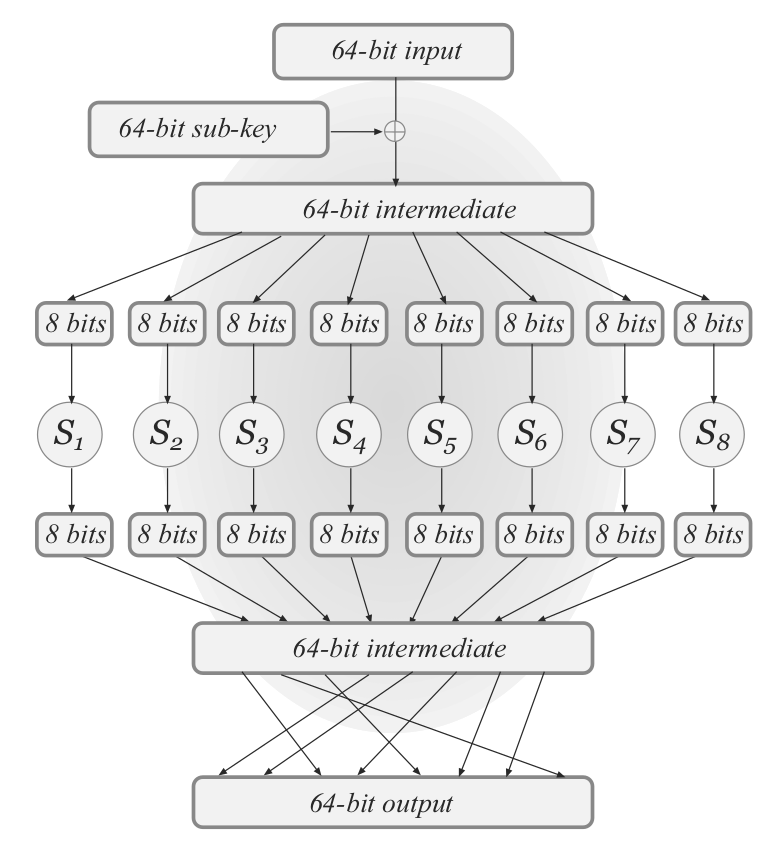
\includegraphics[width=0.5\linewidth]{2024-04-15-spn.png}
\end{center}

We can repeat this procedure for multiple rounds. For example, below is a 3-round SPN.

\begin{center}
    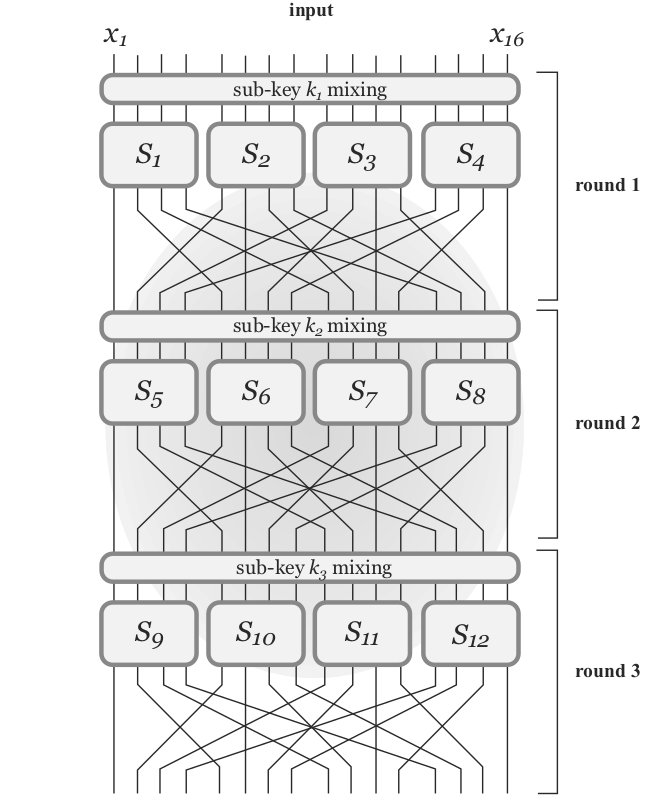
\includegraphics[width=0.5\linewidth]{2024-04-15-spn-mult.png}
\end{center}

Different sub-keys are used in each round. These sub-keys are derived from a \textit{master key} using a \textit{key schedule}, for example, by taking different subsets from the master key.

Given the master key, we can compute $F_{k}^{-1}(y)$. First, use the key schedule to find each sub-key, which we can use to XOR to get the inverse. Then, since each mixing permutation is public, we can compute its inverse for each round. Additionally, each S-box is public, so we can find its inverse too. Thus we have all the information we need to compute the inverse.

\subsection{Attacks on Reduced-Round SPN}

\textbf{1-round SPN without final key mixing.} The adversary can begin with the output $y$, then invert it starting from the end to the beginning. Since the permutations are public, the adversary can compute $x \oplus k$, and since they know the input $x$, they can figure out $k$. Thus we have a complete break. This shows that we need a final key mixing step.

\textbf{1-round SPN with final key mixing.} Assume the key and input is 16-bit. The adversary can try to attack by enumerate the possible values of $k_2$, then using the SPN derive $k_1$ for each $k_2$. This takes $O(2^{16})$ time and gives $2^{16}$ possible values for the master key.

\subsection{Feistel Network}

\begin{center}
    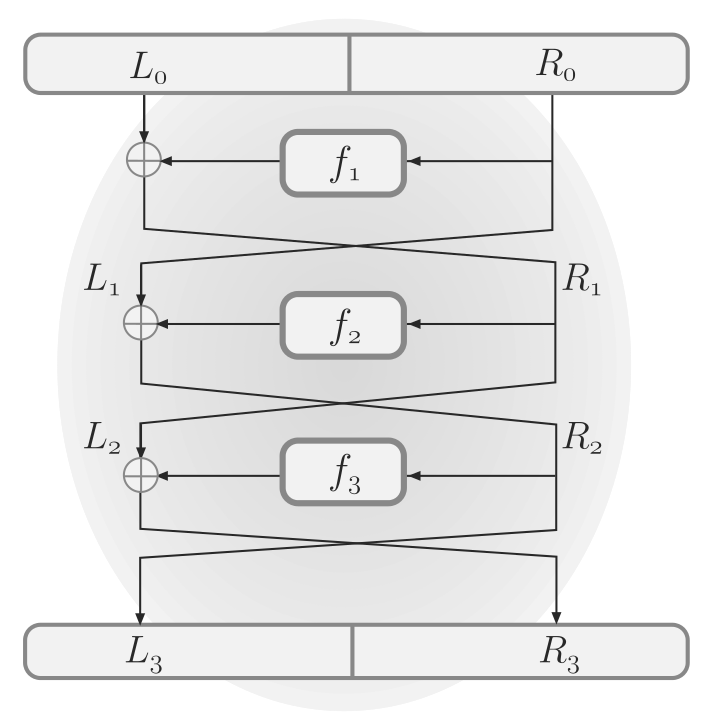
\includegraphics[width=0.5\linewidth]{2024-04-15-feistel-3round.png}
\end{center}

Let $x = L_0 || R_0$ be the input split into two halves, left and right. The $R_0$ is fed into a \textit{round function} $f_1$ and is XOR-ed with $L_0$ to get $R_1$. Then $L_1$ is defined to be $R_0$. This is repeated for several rounds (3 rounds in the figure above). Let $y= L_n || R_n$ be the output after $n$ rounds.

To compute the inverse $F_k^{-1}(y)$, start from the output e.g. $(L_3, R_3)$. We know $R_2 = L_3$, so we can compute $f_3(R_2)$. This satisfies $f_3(R_2) \oplus L_2 = R_3$, so we can find $L_2$. Thus we have found $(L_2, R_2)$, and we can continue until we get $x$.

There are attacks on reduced-round Feistel Networks that we will not cover in lecture, but you can think about it on your own.

\subsection{Data Encryption Standard (DES)}

Recall that the block length is $n=64$ and master key length is $\lambda = 56$ for DES. Use the Feistel network on our $64$-bit input $x$ so that $L_0, R_0$ each get $32$ bits. For the round functions, we use something called a \textit{DES mangler function}, which is essentially a SPN.

However, unlike an SPN, the S-boxes are not permutation, but rather they reduce the size from 6-bit to 4-bit. Additionally, the follow the following properties
\begin{enumerate}
    \item Maps $\{0, 1\}^6 \to \{0, 1\}^4$.
    \item ``4-to-1'': Exactly 4 inputs map to the same output.
    \item 1-bit change of input gives at least 2-bit change in the output.
\end{enumerate}

\begin{center}
    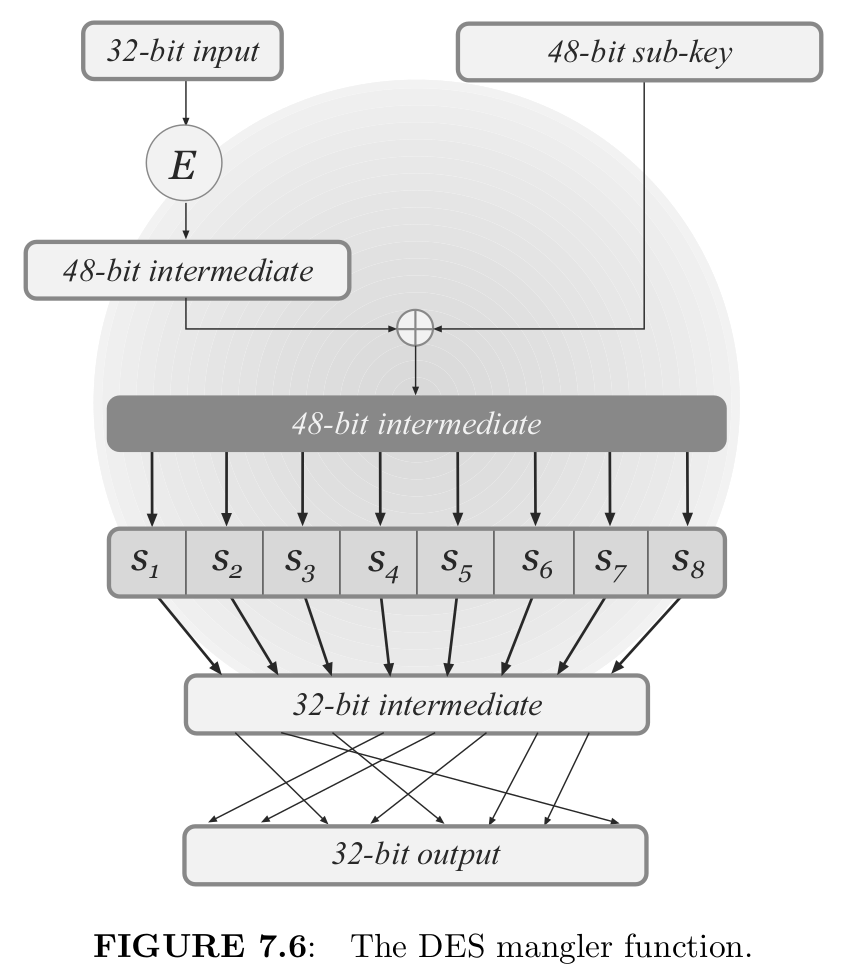
\includegraphics[width=0.5\linewidth]{2024-04-15-dsa-mangler.png}
\end{center}

$E$ is an expansion function. Given a 32-bit string AB where A and B are 16-bit, the output is a 42-bit string ABA.

For the key schedule, we have a master key with length 56 but need a 48-bit sub-key. To do so, split the master key into two halves of 28-bits each, then take a random subset of 24-bits from each half. Then concatenate these two subsets to form a 48-bit sub-key.

\begin{remark}
    DES does seem very complicated. This is intentional to do so so that attacks are hard.

    Multiple rounds of DES does not necessarily improve the security guarantees. Once DES is applied multiple times, we lose our security guarantee, and we need to do additional cryptanalysis, so it is unclear if it is secure. This is the reason NIST developed a new standard known as AES.
\end{remark}
%!TEX root = ../notes.tex
% Scribe: Sudatta Hor
\section{April 17, 2024}
\label{20240417}

This lecture, we will talk about secure hardware and give a brief introduction to blockchain.

\subsection{Outsourcing Computation by FHE}

Recall that by using FHE, we can outsource computation for a server to do while preserving the privacy of the inputs.

\pseudocodeblock{
    \textbf{Server} \< \< \textbf{Client} \\
    \< \< \text{Data }x \text{, Key } \sk \\
    \< \< \ct \gets \Enc(x)\\
    \< \sendmessageleft*{\ct, f} \< \\
    \text{Public Evaluation} \< \< \\
    \ct' \gets \Eval(f, \ct) \< \< \\
    \< \sendmessageright*{\ct'} \< \\
    \< \< f(x) \gets \Dec_{\sk}(\ct')\\
}

Usually, this procedure is very expensive for the server to compute. Instead of using this, there is an alternate solution using \textit{secure hardware}.

\subsection{Outsourcing Computation by Secure Hardware}

Imagine that the server, instead of having all of the computations being public, has an encrypted form of the memory and the CPU. Whatever happens on the server side in the hardware (memory and CPU) is hidden to the server. The hardware is like a secure enclave. This is known as \textit{secure hardware}.

If the client and the secure hardware can agree on a secret key $\sk$ that is hidden from the server, then the server uses the secure hardware to do computation without learning the input. This is much faster than homomorphic encryption.

\pseudocodeblock{
    \textbf{Server} \< \< \textbf{Client} \\
    \< \< \text{Data }x \text{, Key } \sk \\
    \< \< \ct \gets \Enc(x)\\
    \text{Input }(\ct, f) \< \sendmessageleft*{\ct, f}\< \\
    % begin secure hardware box
    \fbox{\begin{subprocedure}\procedure{Secure Hardware}{
        x \gets \Dec_{\sk}(\ct)\\
        y:= f(x)\\
        \pcreturn \ct' \gets \Enc_{\sk}(y)\\
    }\end{subprocedure}} \< \< \\
    % end secure hardware box
    \text{Get }\ct' \< \sendmessageright*{\ct'} \< y \gets \Dec_{\sk}(\ct')\\
}

\subsection{Intel Software Guard Extension (SGX)}

How does the client and the secure hardware agree on the secret key? They must do a key exchange with each other. This is exactly what happens in Intel SGX, also known as ``secure enclave''.

\pseudocodeblock{
    \textbf{Server} \< \< \textbf{Client} \\
    \< \sendmessagerightleft*{\text{DH Key Exchange}} \< \\
    % begin secure hardware box
    \fbox{\begin{subprocedure}\procedure{Enclave}{
        b \gets \ZZ_q\\
        \pcreturn g^b\\
        k := \text{HKDF}(g^{ab})\\
    }\end{subprocedure}} \< \sendmessageleft*{g^a} \< a \sample \ZZ_q \\
    \< \sendmessageright*{g^b} \< k: = \text{HKDF}(g^{ab})\\
    % end secure hardware box
    \text{Input }(\ct, f) \< \sendmessageleft*{\ct, f}\< \\
    % begin secure hardware box
    \fbox{\begin{subprocedure}\procedure{Enclave}{
        x \gets \Dec_{\sk}(\ct)\\
        y:= f(x)\\
        \pcreturn \ct' \gets \Enc_{\sk}(y)\\
    }\end{subprocedure}} \< \< \\
    % end secure hardware box
    \text{Get }\ct' \< \sendmessageright*{\ct'} \< y \gets \Dec_{\sk}(\ct')\\
}

Here, the client does a DH key exchange with the secure enclave by sending $g^a$ to the server, which passes it onto the enclave. Then the enclave returns $g^b$, which the server passes onto the client. However, the is susceptible to a man-in-the-middle attack, where the server is the man-in-the-middle and can send their own $g^{b'}$ to the client instead of $g^b$. To remedy this, we need to use digital signatures so that the enclave can prove to the client that they are certified by Intel.

Every time when you want to compute some function, you need to generate a new certificate. The enclave must run a ``provisioning'' procedure with Intel to receive a new certificate (Intel can charge you here!) and the client must run some ``attestation'' procedure (Intel can charge you here!). It does not have to be as complicated as this, but it is so because there is a business model.

The certificate is also generated on the the function $f$, so that the client ensures that the enclave is computing the correct function.

\textbf{Constraints and Attacks:}

\begin{enumerate}
    \item Need to trust hardware and Intel to do things correctly.
    \item Limited memory size: 128 MB
    \item Replay attacks: although everything is secure against the server, the server can keep a snapshot of everything and replay things on a future input.
    \item Side-channel attacks: it leaks the memory access pattern. When the CPU in the enclave will utilize different blocks of memory, and the server can see the pattern in which the CPU accesses different memory locations. For example, the server might notice that the CPU accesses the same memory location multiple times, which can reveal something about the computation. A fix involves something called ``Oblivous RAM (ORAM)'', which requires $\Theta (\log N)$ memory overhead.
\end{enumerate}

\subsection{Hardware Secure Module (HSM)}

In Intel SGX, you can do arbitrary computations. However, HSM can only do restricted computations, for example, encryption/decryption. Alice can have an HSM that encrypts a message and she sends the encryption to Bob who has an HSM to decrypt the message. Another example is an HSM that takes in a ciphertext, decrypts it, then re-encrypts it with a new secret key.

This is used in places like Visa and a lot of bank systems. This is because they do not want to store the key anywhere, so that the user can only interact with the HSM like a black box without seeing the key.

\textit{How does an encrypt/decrypt HSM pai agree on a key?} The encrypt HSM (Alice) randomly samples $k_1, k_2, k_3$ such that $k_1 \oplus k_2 \oplus k_3 = k$. Then the 3 of them will be mailed to the decrypt HSM (Bob) using 3 different carriers, and the decrypt HSM will reconstruct the key $k$ on its own.

\subsection{Blockchain}

Next, we will talk about Blockchain. First, let's talk about how transactions happens in real life. If Alice wants to buy coffee at Starbucks, she will send \$3 to Starbucks and receive her coffee. Then Alice will make a transaction saying something like ``Alice $\to$ Starbucks \$3'', which is sent to Bank of America. Then Bank of America will verify to things and approve it.

\begin{enumerate}
    \item The transaction is initiated by sender (verify identity).
    \item There is enough balance in the sender's account.
\end{enumerate}

There is a trusted third party (Bank of America) that maintains a \textit{private} ledger that contains all of the transactions.

\begin{center}
\fbox{
    \parbox{0.3\textwidth}{
    \centering
    \fbox{``Alice $\to$ Starbucks \$3''}

    \vspace*{2mm}

    \fbox{``Starbucks $\to$ Bob \$3''}

    \vspace*{2mm}

    $\vdots$

    \vspace*{2mm}
    }
}
\end{center}

Blockchain aims to have a \textit{public} ledger that everyone can view and verify. This is a chain of blocks that are maintained by ``miners'' in a distributed way.

\begin{center}
    \scriptsize
    \def\svgwidth{\linewidth}
    \input{images/2024/.xdp-2024-04-17-blockchain.pdf_tex-COvXWq}
\end{center}

\begin{itemize}
    \item[Step 1.] Charlie wants to make a transaction Charlie $\to$ Starbucks $\bitcoin$3. He broadcasts it to the entire network.
    \item[Step 2.] All miners collect all transactions in the network.
    \begin{itemize}
        \item Verify validity: 1. that the transaction is initiated by the sender and 2. that there is enough balance in the sender's account.
        \item Agree on the next block.
    \end{itemize}
    \item[Step 3.] Repeat.
\end{itemize}

Each block generates some cryptocurrency, which goes to the miner who owns that block. Let's say Alice owns one block that generates one Bitcoin $\bitcoin$3, then Alice gets that one Bitcoin.

\begin{remark}
    The original inventor of Bitcoin had all of the blocks and generate a lot of Bitcoin initially, even when there were no transactions. They likely made a billion dollars and there identity is still unknown.
\end{remark}

\textbf{How do we ensure that the transaction is initiated by the sender?} This can be done using digital signatures. Each party generates a verification/signing key pair. When Bob sends Charlie 5 Bitcoin, he prepares a messages $m_1$ with his verification key, Charlie's verification key, and the amount of Bitcoin that he sends. Bob signs $m$ and creates a certificate $\sigma$. Thus, it is important for each party to hold onto their secret key, or else they will lose their assets.

\textbf{How do we agree on the ledger?} Let's say Charlie wants to make two transactions. Transaction 1, where Charlie sends Starbucks $\bitcoin$3, and transaction 2, where Charlie sends Alice $\bitcoin$4. Let's say that Charlie only has $\bitcoin$5 in his account. Then each transaction is valid by themselves, but together they are not. What we do is have multiple miners, and each of them propose a different block. We want all miners to agree on the same block, and that this new block is valid.

\begin{center}
    \small
    \def\svgwidth{\linewidth}
    \input{images/2024/.xdp-2024-04-17-blockchain-consensus.pdf_tex-f8BXvt}
\end{center}

It is possible for some miners to be malicious. They might lie about their vote or give inconsistent votes. This can be formalized as a \textbf{Byzantine Agreement} problem, which is well studied in distributed systems. We can use the \textbf{Byzantine Fault Tolerance (BFT) Protocol}, which guarantees that it is possible to reach consensus if $n \geq 3t + 1$ where $n$ is the total number of parties and $t$ is the number of malicious parties. In other words, we agree on a valid block if less than a third of the parties are malicious.

However, the problem with this system is that it is ``permissionless''. Thus anyone can become a miner. In particular, there might be an individual who makes a large number of fake accounts so that they make more than a third of the total number of parties. This is known as the ``sybil attack''. The idea to solve this uses Proof of Work (PoW).

\subsection{Proof of Work (PoW)}

Instead of assuming an honest majority of \textit{human beings}, we assume an honest majority of \textit{computational power}. This technique is called Proof of Work. For any miner with a block, they must add something called a ``nonce'' to the block and compute the hash of it (e.g. SHA256). The probability that the first 30 bits of the output is all 0 is $1/2^{30}$. The miner will try a different nonce each time until the first 30 bits are all zero, thus they will try $2^{30}$ times in expectation.

Using this, the consensus protocol is as follows. Whoever first finds a block that hashes to a values with at least 30 leading 0's, then their block becomes the next block.

\begin{remark}
    Here, 30 is just an arbitrary number used just as an example. In practice, a different number may be used.
\end{remark}

There might be a problem with this consensus protocol in which two miners might find the block at the same time, and for example the network delay may be the reason why one finds their block first. If this happens, miner 1 will share their block with half the miners and miner 2 will share their block with the other half. Each half will continue trying to find the next block. If the two miners once again find the next block at the same time, we must repeat this procedure. Otherwise, one miner will find the next block before the others, i.e. find a chain that is longest. We adopt this chain. This is called the ``Longest Chain Rule''. Assuming honest majority of computation power, the longest chain is always valid.

This completes our overview of how Blockchain works. Some final notes:

\begin{itemize}
    \item Efficient verification of sufficient balance: Merkle Tree.
    \item Settlement of a transaction: We need to ensure that a transaction is included in a block which is $\geq 6$ blocks deep ($\sim$ 1 hr), since by the Longest Chain Rule, there may be a longer chain in which the transaction does not exist.
    \item Dynamically adjust the number of leading 0's so that each block takes $\sim$ 10 min to mine. Last 1 hr: \begin{enumerate}
        \item > 6 blocks, increase \# leading 0's
        \item < 6 blocks, decrease \# leading 0's
    \end{enumerate}
    \item Miner's motivation:\begin{enumerate}
        \item Each miner gains a transaction fee
        \item A new coin generated in each block goes to the miner. However, it has been shown that the number of Bitcoin mined will eventually run out. It used to be that each block mined a lot of Bitcoin, but now not so much, and there is a schedule on how much Bitcoin there is left to mine. There are some potential economic issues when all Bitcoins have been mined.
    \end{enumerate}
    \item Extensions \begin{enumerate}
        \item  PoW wastes a lot of power, so Proof of Stake (PoS) is proposed. Here, a miner is sampled proportional to the amount of money they have.
        \item Anonymous transactions (zk-SNARGs). Instead of putting everything public on the chain, you post something that allows you to verify validity in zero-knowledge.
        \item Smart contracts. A client puts a deposit into a distributed third party (miners), and the miners will ensure that the contractor completes the work and give them the payment.
        \item Public Bulletin Board. You can think of the blockchain as a public bulletin board that is not maintained by any central authority, but is handled in a distributed way.
    \end{enumerate}
\end{itemize}




%!TEX root = ../notes.tex
% Scribe: Sudatta Hor
\section{April 22, 2024}
\label{20240422}

In this lecture we will cover differential privacy and elliptic curve cryptography.

\subsection{Differential Privacy}

Let's say that we have a database of sensitive data that we want to make public to others without compromising individual's privacy. For example, there might be a database of medical information that we want to share for medical studies.

\begin{center}
    \begin{tabular}{|c|c|c|c|c|c|c|}
        \hline
        Name & Age & Gender & Race & Weight & ZIP & Disease\\ \hline
        Alice & & & & & &\\ \hline
        Bob & & & & & &\\ \hline
        Charlie & & & & & &\\ \hline
        David & & & & & &\\ \hline
        Emily & & & & & &\\ \hline
        Fiona & & & & & &\\ \hline
    \end{tabular}
\end{center}

One attempt to simply anonymize the data by deleting personally identifiable information (PII) such as the name, date of birth, etc. This might still reveal information about the individual. For example, if you see ``Asian female, age 30, living in Providence'' you might guess it might be Peihan! Although the privacy guarantees may be weak, this is what is being used by HIPAA.

Another attempt is to only answer \textit{aggregate statistics queries}, for example only answering ``How many people in Providence have this disease?''. Hopefully, this reveals less information about the individual.

Our goal is that the output shouldn't enable one to learn anything about an individual. This can be trivially achieved, for example if the output was 0 regardless of the data. Then the output does not reveal any private information of the data, but also does not provide much use. Hence, there is a tradeoff between privacy and utility.

Instead, our goal is that the output shouldn't enable one to learn \textit{much more} about an individual \textit{compared to} one with an output computed without the individual.

\begin{definition}
    For a database $D \in \mathcal{X}^n$, let $M$ be a \textit{randomized mechanism} that takes in $D$ and outputs a randomized output $M(D)$.
    $$D  \to \fbox{M} \to M(D)$$

    \textbf{$\epsilon$-Differential Privacy for M} states that for all neighboring datasets $D_1$ and $D_2$ (neighboring means that they differ in exactly one row), and for all $T \subseteq \text{range}(M)$, we have
    $$\Pr [M(D_1) \in T] \leq e^{\epsilon} \cdot \Pr[M(D_2) \in T].$$
\end{definition}

Intuitively, this states that two neighboring datasets have outputs that have similar probability distributions. If you apply $M$ on $D_1$, it will give you the red distribution, and if you apply $M$ on $D_2$, it will give you the blue distribution. Under the interval $T$, the two distributions are close.

\begin{center}
    \def\svgwidth{0.5\linewidth}
    \input{images/2024/.xdp-2024-04-22-diff-priv-pmf.pdf_tex-VFK3Hm}
\end{center}

This property can be relaxed with the following definition.

\begin{definition}
    \textbf{$\epsilon, \delta$-Differential Privacy for M} states that for all neighboring datasets $D_1$ and $D_2$, and for all $T \subseteq \text{range}(M)$, we have
    $$\Pr [M(D_1) \in T] \leq e^{\epsilon} \cdot \Pr[M(D_2) \in T] {\color{red} + \delta}.$$

    If $\epsilon$ or $\delta$ are large, then this is bad for privacy since the two distributions are allowed to differ more.
\end{definition}

An example of a randomized mechanism that is differentially private is called \textit{randomized response}.

\subsubsection{Randomized Response}

Let's say that we want to find the percentage of individuals that satisfy a predicate P. For example, the predicate could be ``is a MATH-CS concentrator''. Then the randomized response algorithm does the following.

\pseudocodeblock{
    \text{For each row }x_i:\\
    \quad 1.\ b \sample \{0, 1\}\\
    \quad 2.\ \text{If } b=0, \text{ then }y_i := P(x_i).\\
    \quad \quad \text{Otherwise, }y_i \sample \{0, 1\}\\
    M(D) := (y_1, \dots, y_n)
}

For example, if we want to find how many students are MATH-CS concentrators, for each student, we will decide to accurately report whether they are a concentrator if $b=0$. Otherwise, if $b=1$, we will just report a random value. Thus, half of the output is the actual response while the other half is just random.

\textbf{Thm:} Randomized response is $\ln 3$-differential private.

\textit{How to estimate the query output $\alpha$?} Let's say that $\alpha$ is the true percentage that satisfies $P$, and that we observe $k$ many 1's in the output. Then $k$ should be approximately
$$k \sim \frac{n}{2}\cdot\frac{1}{2} + \frac{n}{2}\cdot \alpha$$
since roughly half of individuals give random results and half of individuals give true results. Using this, we can approximate $\alpha$ from $k$.

\textit{How to make the mechanism more private?} If we want more privacy, we can adjust the distribution that $b$ is sampled from. We can adjust $b$ to be sampled as $0$ less often, thus the probability that individuals are revealing their true response is lower. Observe that if $b=0$ with probability 1, then we have a completely accurate output at the loss of privacy. If $b=0$ with low probability, then the accuracy of our output is low, but we gain privacy.

\subsubsection{Laplace Mechanism}

The Laplace mechanism is another mechanism that is popular in practice. This can compute an arbitrary real-valued function. This utilizes a notion called \textit{sensitivity} of a function.

\begin{definition}
    The \textbf{sensitivity} $\Delta f$ of a function $f: \mathcal{X}^n \to \mathbb{R}$ is defined as
    $$\Delta f := \max_{D_1 \sim D_2}|f(D_1) - f(D_2)|.$$

    $D_1\sim D_2$ means that $D_1$ and $D_2$ are neighbors.
\end{definition}

The Laplace mechanism is very simple. It justs computes $f$ and adds some noise onto it. For this reason, it is one of the most employed mechanism in practice.

\begin{definition}
    The \textbf{Laplace mechanism} is defined to be
    $$M(D) = f(D) + \text{Lap}(\Delta f / \epsilon)$$
\end{definition}

Here, Lap$(b)$ gives the Laplace distribution whose probability density function (PDF) is given by 
$$\text{PDF}(x) := \frac{1}{2b} \cdot \exp\left(-\frac{|x|}{b}\right).$$
For $x \sim \text{Lap}(b)$, we have that $\Pr [|x| \geq bt] \leq \exp (-t)$.

Below is a plot of PDF for different values of $b$.

\begin{center}
    \def\svgwidth{0.5\linewidth}
    \input{images/2024/.xdp-2024-04-22-laplace-pdf.pdf_tex-ei4hPu}
\end{center}

\textit{Is a bigger $b$ better for privacy, or worse?} A higher $b$ gives better privacy. Intuitively, the PDF becomes wider, so the $\text{Lap}(\Delta f / \epsilon)$ term becomes more random.

\begin{theorem}[Post-processing]
    If $M: X^n \to Y$ is $(\epsilon, \delta)$-differentially private, and $f:Y\to Z$ is an arbitrary randomized function, then $f\circ M : X^n \to Z$ is also $(\epsilon, \delta)$-differentially private.
\end{theorem}

\begin{theorem}[Group privacy]
    If $M: X^n \to Y$ is $(\epsilon, 0)$-differentially private, then $M$ is $(k\cdot \epsilon, 0)$-differentially private for groups of size $k$.

    In the standard definition of differential privacy, we consider two databases that differ by at most one row. However, in some cases, we may want to have a group of databases. Intuitively, you apply $M$ k times between each database, and each time you will lose $\epsilon$ privacy. In total, you lose $k \cdot \epsilon$ privacy.
\end{theorem}

\begin{theorem}[Composition]
    If $M_i: X^n \to Y$ is $(\epsilon_i, \delta_i)$-differentially private for $i = 1, \dots, k,$ then
    $$M(D) := (M_1(D), \dots, M_k(D))$$
    is $(\sum \epsilon_i, \sum \delta_i)$-differentially private.
\end{theorem}

\subsection{Elliptic Curve Cryptography}

So far, we have primarily been working with cyclic group $G$ of order $q$ with generator $g$ where DLOG/CDH/DDH holds. How large is $q$?
\begin{itemize}
    \item For integer groups, $q \sim 2048$ bits.
    \item For elliptic curve groups, $q \sim 256$ bits.
\end{itemize}
Thus, elliptic curve groups are more space-efficient for cryptography! The known attacks for elliptic curve groups scale on the order of $\sqrt{q}$, which allows us to have a smaller $q$ parameter to ensure security.

\begin{definition}
    An \textbf{elliptic curve} is the set of solutions $(x,y)$ to the equation
    $$y^2 = x^3 + ax + b$$
    where $4a^3 + 27b^2 \neq 0$. The last condition is there so that we get the elliptic curve shape.
\end{definition}

\begin{example}
    The elliptic curve to $y^2 = x^3 - x + 9$ is has a plot that looks something like the following. The solutions $(0, \pm 3), (1, \pm 3), (-1, \pm 3)$ are indicated with dots.

    \begin{center}
    \footnotesize
    \def\svgwidth{0.35\linewidth}
    \input{images/2024/.xdp-2024-04-22-elliptic-curve.pdf_tex-giJsNo}
    \end{center}
\end{example}

\textit{How to find rational points $(x,y) \in \mathbb{Q}^2$ on the curve?} There are two ways, the chord method and the tangent method.
\begin{enumerate}
    \item \textbf{Chord method:} Given a point P and a point Q on the curve, it defines a line $PQ$. This line must intersect the curve in a third point, R. For the curve in the previous example, if $P=(-1, -3)$ and $Q=(1, 3)$, then this defines a line $y=3x$. Plugging this into the equation for the curve gives us
    $$(3x)^2 = x^3 - x + 9.$$
    This is a cubic equation, so there must be 3 roots and thus 3 intersections. We know that the product of the roots must be negative the constant term, so $a_1 a_2 a_3 = -9$. We know two of the roots $a_1 = 1$ and $a_2 = -1$, so we have that $a_3 = 9$, which gives us the third point $R = (9, 27)$.

    We define this operation by $P \boxplus Q = R$. Notice that if $P, Q$ are rational points, then $R$ is rational because all of our steps to find $R$ is just multiplying, dividing, adding, and subtracting with rational numbers.

    \begin{center}
        \def\svgwidth{0.35\linewidth}
        \input{images/2024/.xdp-2024-04-22-elliptic-curve-chord.pdf_tex-JXGUox}
    \end{center}


    \pagebreak
    \item \textbf{Tangent method:} Imagine if the cubic equation had a double root. This corresponds to a point $P$ being the tangent point to the line. In this case, we apply the operation onto itself $P \boxplus P = S$.

    \begin{center}
        \def\svgwidth{0.35\linewidth}
        \input{images/2024/.xdp-2024-04-22-elliptic-curve-tangent.pdf_tex-B29VSo}
    \end{center}
\end{enumerate}

Geometrically, one can be convinced that $(P \boxplus Q) \boxplus X = P \boxplus (Q\boxplus X)$ and that $P \boxplus Q = Q \boxplus P$. This gives hope that we can construct a group out of this, which is very handy for cryptography!

\begin{definition}
    For prime $p >3$, let $\mathbb{F}_p$ be a finite field, i.e. all of the integers $\{0, 1, \dots, p-1\}$ with addition and multiplication. Let $a, b \in \mathbb{F}_p$ such that $4a^3 + 27b^2 \neq 0$.
    
    An \textbf{elliptic curve $E$ defined over $\mathbb{F}_p$}, denoted $E / \mathbb{F}_p$, is the set of all points $(x,y)$ such that
    \begin{itemize}
        \item $x,y \in \mathbb{F}_p$ and
        \item $y^2 = x^3 + ax +b$
    \end{itemize}

    Additionally, we include an abstract element $\mathcal{O}$ that is thought of as the ``point at infinity''.
\end{definition}

\begin{example}
    $y^2 = x^3 + 1$ over $\mathbb{F}_{11}$ consists of the points
    $$E / \mathbb{F}_{11} = \{\mathcal{O}, (-1, 0), (0, \pm 1), (2, \pm 3), (5, \pm 4), (7, \pm 5), (9, \pm 2)\}$$
\end{example}

Elliptic curves over finite fields is the same definition as elliptic curves before except we restrict our attention to $\mathbb{F}_p$.

\begin{proposition}
    Elliptic curves over finite fields with the $\boxplus$ operation form a group.
    \begin{enumerate}
        \item \textbf{Closure:} $\forall g, h \in G, g\boxplus h \in G$. This is true because $g,h$ defines a line, and we can figure out the equation for this line over the finite field because finite fields support division. After we find the line, we can plug it into the curve equation to get a cubic equation. We have two roots, and we know the product of all of the roots is negative the constant term in the cubic equation. Since finite fields support division, we can recover the third root.
        \item \textbf{Existence of identity:} $\exists e \in G $ such that $\forall g\in G, e \boxplus g = g \boxplus e = g$. We let $e = \mathcal{O}$ be the identity. 
        \item \textbf{Existence of inverse:} $\forall g \in G, \exists h \in G, $ such that $g \boxplus h = h \boxplus g = e$. If $g = (x,y)$, then the inverse $h = (x, -y)$. You can see that drawing a line between $g,h$ gives us the point at infinity, so $g \boxplus h = \mathcal{O}$.
        \item \textbf{Associativity:} $\forall g_1, g_2, g_3 \in G, (g_1 \boxplus g_2) \boxplus g_3 = g_1 \boxplus (g_2 \boxplus g_3)$. We discussed this earlier.
        \item \textbf{Commutativity (for abelian groups):} $\forall g,h \in G, g\boxplus h = h \boxplus g.$ We discussed this earlier.
    \end{enumerate}
\end{proposition}

Furthermore, the \textbf{SEA algorithm} can count the number of points on $E / \mathbb{F}_p$ in polylog(p) time. Thus, figuring out the order of the group does not give us a problem.

Below are some curves that are standardized and used in practice. We only talk about the first one. The others are secure to use in practice and have some tradeoffs that you are welcome to look into.

\begin{itemize}
    \item curve secp2546r1 (P256) \begin{itemize}
        \item Prime $p = 2^{256} - 2^{224} + 2^{192} + 2^{96} -1$, hence only needs 256 bits to store!
        \item $y^2 = x^3 -3x + b$ for some constant $b$ that is a 255-bit string.
        \item Number of points on the curve is prime (close to p).
        \item Standardized generator point $G$. It does not have to be this particular $G$, since every point is a generator, but it is standardized so that everyone can agree on the generator to run DH key exchange for example.
    \end{itemize}
    \item curve secp256k1
    \item curve 25519
\end{itemize}

\end{document}